\chapter[ $ \ \ $ АНАЛИЗ $ \ \ \ $ ЭФФЕКТИВНОСТИ $ \ \ \ $ РАБОТЫ $ \ \ \ $ ПРЕДЛОЖЕННОГО $ \ \ $ БУФЕРА $ \ \ $ КОМПЕНСАЦИИ $ \ \ $ ДЖИТТЕРА $ \ $ С $ \ $ ОСНОВНЫМИ $ \ $ ИСТОЧНИКАМИ $ \ $ ДЖИТТЕРА В ГИБРИДНЫХ СЕТЯХ]{АНАЛИЗ ЭФФЕКТИВНОСТИ РАБОТЫ ПРЕДЛОЖЕННОГО БУФЕРА КОМПЕНСАЦИИ ДЖИТТЕРА С ОСНОВНЫМИ ИСТОЧНИКАМИ ДЖИТТЕРА В ГИБРИДНЫХ СЕТЯХ} \label{chapt4}
%В данном разделе проведем сравнение предложенного алгоритма буфера основанного на ГРФК (\ref{eq3:skachok},\ref{eq3:vibros}), описанного в разделе \ref{sect3_5} с алгоритмом буфера (\ref{eq3:playout}-\ref{eq3:playout_v}) из \cite{Ramjee}. С константами $\gamma=4$ и $\Delta t=5$.



\nomenclature{EPC}{Evolved Packet Core}
\nomenclature{PHY}{Physical layer}
\nomenclature{MAC}{Media access control}
\nomenclature{NS2}{Network Simulator 2}
\nomenclature{МСЭ}{Международный Союз Электросвязи}
\nomenclature{TOTEM}{TOolbox for Traffic Engineering Methods}
\nomenclature{EQRS}{Extended QoS-based Routing Simulator}
\nomenclature{MaRS}{Maryland Routing Simulator}
\nomenclature{RRC}{Radio Resource Control}
\nomenclature{PDCP}{Packet Data Convergence Protocol}
\nomenclature{RLC}{Radio Link Control}
\nomenclature{UE}{User Equipment}
\nomenclature{eNB}{evolved Node B}
\nomenclature{S-GW}{Serving Gateway}
\nomenclature{P-GW}{Packet Data Network Gateway}
\nomenclature{MME}{Mobility Management Entity}
\nomenclature{3GPP}{3rd Generation Partnership Project}
\nomenclature{GTP}{GPRS Tunnelling Protocol}
\nomenclature{UDP}{User Datagram Protocol}
\nomenclature{IP}{Internet Protocol}
\nomenclature{TFT}{Traffic Flow Template}
\nomenclature{ePS}{evolved Packet System}
\nomenclature{TEID}{Tunnel Endpoint ID}
\nomenclature{RBID}{Radio Bearer ID}



Одним из важнейших этапов в ходе разработки математической модели джиттера задержки прибытия пакетов и методов компенсации джиттера являются экспериментальные исследования этих решений.
Содержание подобных исследований удобно представить в виде следующих частных задач:
\begin{itemize}
 \item анализ эффективности буфера компенсации джиттера в ситуации изменения маршрута передачи пакетов;
 \item анализ эффективности буфера компенсации джиттера в ситуации хэндовера между базовыми станциями;
 \item анализ эффективности буфера компенсации джиттера в ситуации перегрузки в сети;
 \item анализ эффективности буфера компенсации джиттера в ситуации увеличения расстояния между базовой станцией и абонентом в сети LTE;
 \item анализ эффективности буфера компенсации джиттера в ситуации внутрисистемных помех;
 \item Выработка рекомендаций по практическому применению разработанных методов компенсации джиттера в сетях LTE.
\end{itemize}
При решении поставленной задачи для получения наиболее точной информации о функционировании предложенного алгоритма буфера компенсации джиттера используются методы имитационного моделирования.
Для анализа эффективности предложенных методов компенсации джиттера (\ref{eq3:skachok},\ref{eq3:vibros}), описанных в третьем и четвертом разделе, проведем сравнение с классическим адаптивным алгоритмом буфера компенсации джиттера (\ref{eq3:playout}-\ref{eq3:playout_v}), который описан в первом разделе \cite{Ramjee}. 
Для моделирования использовались следующие входные данные $\gamma=4$ и $\Delta t=5$.


\section{Описание имитационного эксперимента по исследованию джиттера в сетях LTE}

С целью проверки эффективности предложенных сетевых решений обычно применяются средства аналитического и имитационного моделирования и натурного или лабораторного эксперимента.
Причем в рамках средств аналитического моделирования используются программные пакеты MatLab, Octave, MathCad, Maple \cite{matlab,octave,mathcad,maple}, 
имитационного --- NS2 (Network Simulator 2), NS3 (Network Simulator 3) \cite{ns3}, TOTEM (TOolbox for Traffic Engineering Methods), 
EQRS (Extended QoS-based Routing Simulator), MaRS (Maryland Routing Simulator).
Эти специализированные пакеты позволяют достаточно точно отобразить функционирование телекоммуникационной сети или отдельных ее процессов.

Рассмотрим более детально инструмент имитационного моделирования NS3.
NS3 представляет собой симулятор дискретных событий сети, который ориентирован в первую очередь для научных исследований и образовательных целей. 
NS3 является свободным программным обеспечением под лицензией GNU GPLv2, и находится в открытом доступе для исследований, разработки и использования.

NS3 проект стремится к созданию твердого ядра ​​моделирования, которое хорошо документировано, простое в использование и отладке, и которое обеспечивает потребности всего рабочего процесса моделирования, от моделирования до сбора и анализа данных.
Кроме того, NS3 программная инфраструктура способствует развитию имитационных моделей, которые являются достаточно реалистичными, чтобы использовать NS3 в качестве эмулятора сети в реальном времени.
NS3 симулятор поддерживает моделирование как проводных, так и беспроводных сетей, тем не менее, подавляющее большинство разрабатываемых моделей сфокусировано на моделировании беспроводных IP сетей, которые включают модели для Wi-Fi, WiMAX и LTE.


Опишем имитационную модель эксперимента для исследования джиттера в сетях LTE.
Обзор имитационной модели LTE-EPC изображен на рис. \ref{img:LTEEPC}. Состоит из двух основных компонентов:
\begin{itemize}
  \item Модель LTE. Эта модель включает LTE радио стек протоколов (RRC, PDCP, RLC, MAC, PHY). Эти объекты полностью находятся на UE и eNB узлах.
  \item Модель EPC. Эта модель включает в себя основные сетевые интерфейсы, протоколы и объекты. Эти объекты и протоколы находятся на S-GW, P-GW и MME узлах и частично на eNB узлах.
\end{itemize}

\begin{figure} [h]
  \center
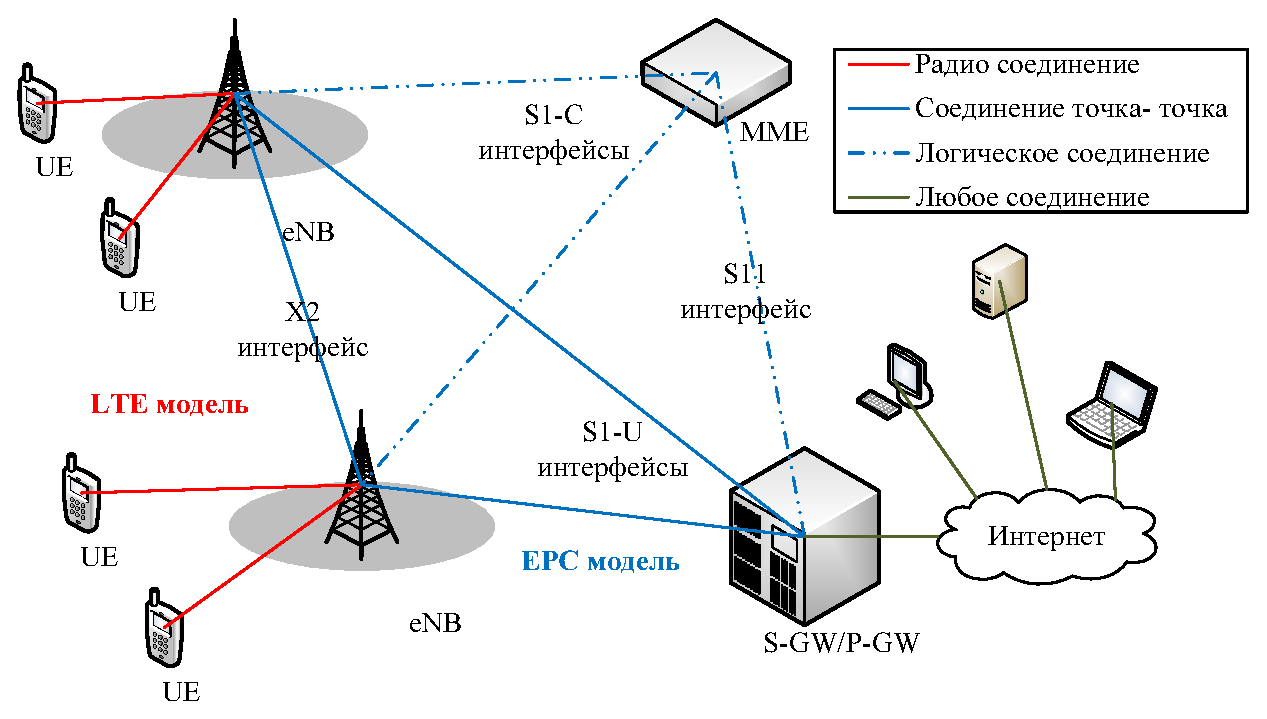
\includegraphics [width=0.95\textwidth] {LTEEPC.eps}
  \caption{Обзор имитационной модели LTE-EPC \cite{LteSimDoc}}
  \label{img:LTEEPC}
\end{figure}



\subsection{Обзор архитектуры LTE модели в сетевом сумуляторе NS3} \label{B1}
LTE модель была разработана для поддержки оценки следующих аспектов системы LTE:
\begin{itemize}
  \item Управление радио ресурсами.
  \item Пакетная обработка на основе QoS.
  \item Внутрисистемные помехи между сотами.
  \item Динамический спектральный доступ
\end{itemize}


Архитектура физического и канального уровня для модели узла UE представлена на рис. \ref{img:UEPHY} и для модели узла eNB представлена на рис \ref{img:eNBPHY}.
\begin{figure} [h]
  \center
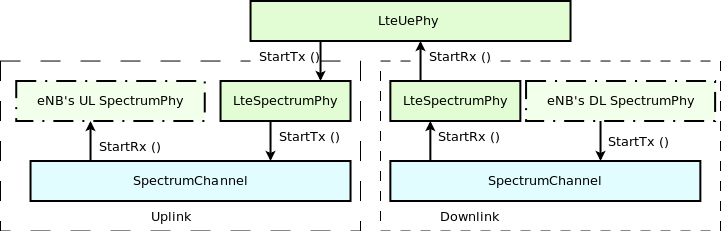
\includegraphics [width=0.95\textwidth] {UEPHY.png}
  \caption{Архитектура физического и канального уровня для модели UE \cite{LteSimDoc}}
  \label{img:UEPHY}
\end{figure}

\begin{figure} [h]
  \center
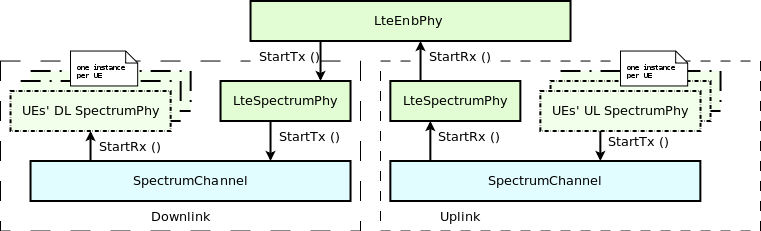
\includegraphics [width=0.95\textwidth] {eNBPHY.png}
  \caption{Архитектура физического и канального уровня для модели eNB \cite{LteSimDoc}}
  \label{img:eNBPHY}
\end{figure}

\subsection{Обзор архитектуры EPC модели в сетевом сумуляторе NS3} \label{B2}
Модели EPC обеспечивают средства для моделирования сквозного IP соединения поверх LTE модели. 
В частности, поддерживают соединение нескольких UE с интернетом через сеть радиодоступа с несколькими узлами eNB, подключенными к одному S-GW/P-GW узлу. 
Эта топология сети изображена на рис \ref{img:LTEEPCdata}.
Основное внимание в модели ЕРС в настоящее время сфокусировано на плоскости данных EPC. 
Чтобы понять архитектуру этой модели, необходимо ознакомиться с рис. \ref{img:LTEEPCdata}, где представлен сквозной LTE-EPC стек протоколов, таким образом, каким это реализовано в симуляторе. 
Из рисунка видно, что самым большим упрощением, введенным в модель ЕРС для плоскости данных, является включение функций S-GW и P-GW в один узел S-GW/P-GW, который устраняет необходимость S5 или S8 интерфейсов, определенных в 3GPP. 
С другой стороны, все уровни протокола S1-U и протокола радиосвязи LTE стека, указанные в 3GPP, присутствуют.

\begin{figure} [h]
  \center
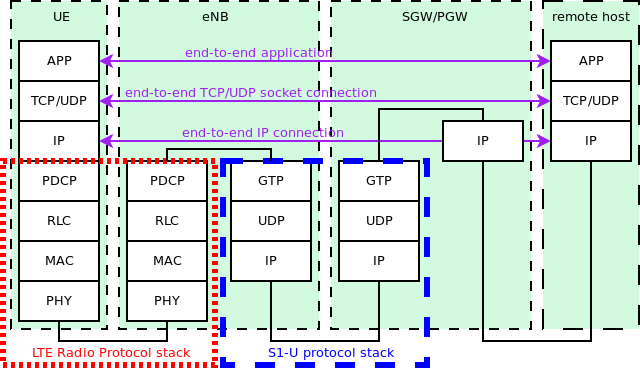
\includegraphics [width=0.95\textwidth] {LTEEPCdata.png}
  \caption{Архитектура физического и канального уровня для модели eNB \cite{LteSimDoc1}}
  \label{img:LTEEPCdata}
\end{figure}

Как показано на рисунке, существует два различных уровня IP-сети. 
Первый это сквозной уровень, который обеспечивает сквозное подключение к пользователям; этот уровень включает UE, P-GW и удаленный хост (в том числе возможные интернет маршрутизаторы и хосты между ними), но не включает eNB.
По умолчанию, UE присваивается публичный адрес IPv4 из 7.0.0.0/8 сети и P-GW присваивается адрес 7.0.0.1, который используется всеми UE, в качестве шлюза для доступа в Интернет.
Второй слой IP сетей является eNB локальной сетью, которая включает в себя все узлы eNB и S-GW/P-GW узел. 
Эта сеть реализована в виде набора соединений точка-точка, которые соединяют каждый eNB с S-GW/P-GW узлом, таким образом, S-GW/P-GW имеет набор устройств точка-точка, каждый из которых обеспечивает подключение к другому eNB. 
По умолчанию, подсеть 10.xyz/30 присваивается каждому соединению точка-точка.
Как указано в 3GPP, сквозные IP соединения являются туннелями через локальную EPC IP сеть с использованием GTP/UDP/IP. 
Далее рассмотрим, как это туннелирование реализовано в модели ЕРС. Объяснение сделано путем обсуждения сквозного потока пакетов данных.

Для начала, рассмотрим случай нисходящей линии связи, который изображен на рис \ref{img:DownloadUE}. 
IPv4 пакеты нисходящей линии связи генерируются от общего удаленного хоста и адресуются к одному из устройств UE. 
Интернет маршрутизация будет заботиться о пересылке пакета на публичный сетевой интерфейс NetDevice узла S-GW/P-GW, который подключен к Интернету (этот интерфейс Gi в соответствии с 3GPP терминологией). 
S-GW/P-GW имеет сетевой интерфейс VirtualNetDevice которому присваивается IP-адрес шлюза для подсети UE, следовательно, правило статической маршрутизации приведет к тому, 
что входящий пакет из Интернета будут проходить через VirtualNetDevice. 
Это сетевое устройство начинает GTP/UDP/IP туннельную процедуру, путем пересылки пакетов на выделенное приложение на узле S-GW/P-GW, которое называется EpcSgwPgwApplication. Это приложение выполняет следующие операции:



\begin{sidewaysfigure} 
\centering
\begin{tikzpicture} 
[align=center,node distance=2cm]
        \matrix (m1) [row sep=20mm, column sep=3mm] {
		%--------------------------------------------------------------------
		\node[dspfilter,minimum width=3cm] (m00) {Приложение};    &
		\node[dspfilter,minimum width=3cm,text height=3em]                  (m01) {EpcEnb\\Application};          &
		\node[coordinate]                  (m02) {};          &
		\node[coordinate]                  (m03) {};          &
		\node[coordinate]                  (m04) {};          &
		\node[dspfilter,minimum width=3cm,text height=3em]                  (m05) {EpcSgwPgw\\Application};          &
		\node[coordinate]                  (m06) {};          \\
		%--------------------------------------------------------------------
		\node[dspfilter,minimum width=3cm]                  (m10) {IPv4};          &
		\node[dspfilter,minimum width=3cm]                  (m11) {IPv4};          &
		\node[dspfilter,minimum width=3cm]                  (m12) {IPv4};          &
		\node[dspfilter,minimum width=3cm]                  (m13) {IPv4};          &
		\node[dspfilter,minimum width=3cm]                  (m14) {IPv4};          &
		\node[dspfilter,minimum width=3cm]                  (m15) {IPv4};          &
		\node[dspfilter,minimum width=3cm]                  (m16) {Интернет};          \\

		%--------------------------------------------------------------------
		\node[dspfilter,minimum width=3cm,text height=3em]                  (m20) {LteUe\\NetDevice};          &
		\node[dspfilter,minimum width=3cm,text height=3em]                  (m21) {LteEnb\\NetDevice};          &
		\node[dspfilter,minimum width=3cm,text height=3em]                  (m22) {S1-U P2P \\NetDevice};          &
		\node[dspfilter,minimum width=3cm,text height=3em]                  (m23) {S1-U P2P \\NetDevice};          &
		\node[dspfilter,minimum width=3cm,text height=3em]                  (m24) {TUN Virtual \\NetDevice};          &
		\node[dspfilter,minimum width=3cm]                  (m25) {NetDevice};          &
		\node[coordinate]                  (m26) {};          \\
	};
	
	\node[draw,inner xsep=16mm, inner ysep=43mm,dashed,fit=(m00) (m01),label=above:{UE узел}] at (m10) {};
	\node[draw,inner xsep=32.5mm, inner ysep=43mm,dashed,fit=(m00) (m01),label=above:{eNB узел},xshift=16.5mm] at (m11) {};
	\node[draw,inner xsep=49mm, inner ysep=43mm,dashed,fit=(m00) (m01),label=above:{SGW/PGW узел}] at (m14) {};
	
	%\begin{scope}[start chain]
	 %\chainin (m16);
	 %\chainin (m26) [join=by dspline];
	%\end{scope}

\path[>=latex,->] (m16.south) edge[bend  left=40] node[below] {} (m25.east);
\path[>=latex,->] (m25.north) edge[bend  right=45] node[below] {} (m15.east);
\path[>=latex,->] (m15.south) edge[bend  right=25] node[below] {} (m24.north);

\path[>=latex,->] (m24.south) edge[bend  right=135]  node[below] {} (m05.30);
\path[>=latex,->] (m05.south) edge[bend  right=25] node[below] {} (m14.north);
\path[>=latex,->] (m14.north) edge[bend  right=25] node[below] {} (m13.north);
\path[>=latex,->] (m13.south) edge node[below] {} (m23.north);
\path[>=latex,->] (m23.south) edge[bend  left=90] node[below] {} (m22.south);
\path[>=latex,->] (m22.north) edge node[below] {} (m12.south);
\path[>=latex,->] (m12.north) edge[bend  right=45] node[below] {} (m01.east);
\path[>=latex,->] (m01.south) edge node[below] {} (m11.north);
\path[>=latex,->] (m11.south) edge node[below] {} (m21.north);
\path[>=latex,->] (m21.south) edge[bend  left=90] node[below] {} (m20.south);
\path[>=latex,->] (m20.north) edge node[below] {} (m10.south);
\path[>=latex,->] (m10.north) edge node[below] {} (m00.south);


\end{tikzpicture}
\caption{Поток данных нисходящей линии связи между интернетом и узлом UE \cite{LteSimDoc1}}
\label{img:DownloadUE}
\end{sidewaysfigure}



%\begin{figure} [h]
%%  \center
%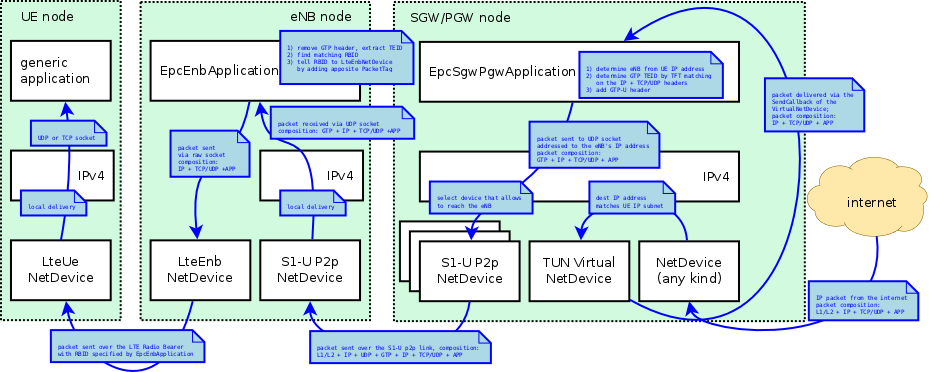
\includegraphics [width=0.95\textwidth] {DownloadUE.png}
%  \caption{Поток данных нисходящей линии связи между интернетом и узлом UE \cite{LteSimDoc1}}
%  \label{img:DownloadUE}
%\end{figure}


\begin{enumerate}
  \item Определяет eNB узел, к которому присоединен UE, смотря на IP-адрес назначения (который является адресом UE).
  \item Классифицирует пакеты, используя шаблоны транспортных потоков (TFT - Traffic Flow Templates), чтобы идентифицировать, какому ePS каналу он принадлежит. ePS каналы имеют карту соответствия к S1-U каналам, так что эта операция возвращает идентификатор TEID (GTP-U Tunnel Endpoint Identifier), к которому принадлежит данный пакет.
  \item Добавляет соответствующие GTP-U-заголовки к пакету.
  \item Отправляет пакет через UDP-сокет к S1-U P2P NetDevice, адресуя к eNB, с которым соединен UE.
\end{enumerate}

Как следствие, пакет со сквозным IP заголовком с добавленными IP, 
UDP и GTP заголовками отправляется через S1 соединение к eNB, 
где он принимается и доставляется локально (в качестве адреса назначения подставляется приватный адрес eNB). Локальный процесс доставки отправит пакет через UDP сокет к выделенному приложению EpcEnbApplication. 
Это приложение выполняет следующие операции:

\begin{enumerate}
  \item Удаляет заголовок GTP и извлекает TEID, который содержится в нем.
  \item Используя взаимно-однозначное соответствие между S1-U каналами и радиоканалами (который является 3GPP требованием), определяет идентификатор радиоканала (RBID -Radio Bearer ID), к которому принадлежит данный пакет.
  \item Записывает RBID в выделенном теге под названием LteRadioBearerTag, который добавляется к пакету.
  \item Пересылает пакет к приложению LteEnbNetDevice eNB узла через raw сокет.
\end{enumerate}
Следует отметить, что в этот момент, внешним заголовком пакета является сквозной IP заголовок, поскольку IP/UDP/GTP заголовки S1 стека протоколов уже были удалены. 
После приема пакета от EpcEnbApplication, LteEnbNetDevice будет извлекать RBID из LteRadioBearerTag, и на основе RBID определит номер радиоканала (и соответствующие PDCP и RLC экземпляры протокола), 
который затем используется для передачи пакета к UE через радиоинтерфейс LTE. 
В конце, приложение LteUeNetDevice узла UE получит пакет и доставит его локально через IP стек протоколов, 
которые в свою очередь доставит его к приложению на узле UE, которое является конечной точкой нисходящей линии связи.

В случае восходящего соединения, показанного на рис. \ref{img:UploadUE} , IP пакеты создаются приложением внутри UE, и передаются через локальный стек протоколов TCP/IP к приложению LteUeNetDevice узла UE. 
LteUeNetDevice затем выполняет следующие операции:

\begin{enumerate}
  \item Классифицирует пакет, используя TFT, и определяет радиоканал, к которому принадлежит пакет (и соответствующий RBID).
  \item Определяет соответствующий экземпляр протокола PDCP, который является точкой входа LTE стека протоколов для этого пакета.
  \item Посылает пакет к eNB через LTE радио стек протоколов.
\end{enumerate}

eNB принимает пакет через его сетевой интерфейс LteEnbNetDevice. 
Поскольку существует один экземпляр протокола PDCP и RLC для каждого радиоканала, LteEnbNetDevice способен определить RBID пакета. 
Это RBID затем записывается в LteRadioBearerTag, который добавляется к пакету. 
LteEnbNetDevice затем пересылает пакет EpcEnbApplication через сокет пакета.
При получении пакета EpcEnbApplication выполняет следующие операции:

\begin{enumerate}
  \item Извлекает RBID из тега LteRadioBearerTag в пакете.
  \item Определяет соответствующий ePS канал и GTP-U TEID за счет использования взаимно-однозначного соответствия между S1-U каналами и радиоканалами.
  \item Добавляет GTP-U заголовок пакета, в том числе TEID, который был определен ранее.
  \item Посылает пакет на S-GW/P-GW узел через UDP сокет подключенный к S1-U сетевому точка-точка устройству.
\end{enumerate}

В этот момент пакет содержит S1-U IP, UDP и GTP заголовки в дополнение к первоначальному сквозному IP заголовку. 
Когда пакет поступает на соответствующий S1-U P2P NetDevice на узле S-GW/P-GW, он доставляется локально. 
Локальный процесс доставки направляет пакет к EpcSgwPgwApplication через соответствующий UDP сокет. 

EpcSgwPgwApplication затем удаляет заголовок GTP и пересылает пакет на VirtualNetDevice. 
На данный момент, внешним заголовком пакета является сквозной IP заголовок. 
Следовательно, если адрес назначения в этом заголовке является удаленным узлом в интернете, пакет отправляется в интернет через соответствующее сетевое устройство NetDevice на узле S-GW/P-GW. 
В случае, если пакет адресован другому UE, IP стек S-GW/P-GW перенаправит пакет снова к сетевому устройству VirtualNetDevice, и пакет будет проходить процесс доставки через нисходящее соединение для того, чтобы достичь пункта назначения UE.


\begin{sidewaysfigure} 
\centering
\begin{tikzpicture} 
[align=center,node distance=2cm]
        \matrix (m1) [row sep=20mm, column sep=3mm] {
		%--------------------------------------------------------------------
		\node[dspfilter,minimum width=3cm] (m00) {Приложение};    &
		\node[dspfilter,minimum width=3cm,text height=3em]                  (m01) {EpcEnb\\Application};          &
		\node[coordinate]                  (m02) {};          &
		\node[coordinate]                  (m03) {};          &
		\node[coordinate]                  (m04) {};          &
		\node[dspfilter,minimum width=3cm,text height=3em]                  (m05) {EpcSgwPgw\\Application};          &
		\node[coordinate]                  (m06) {};          \\
		%--------------------------------------------------------------------
		\node[dspfilter,minimum width=3cm]                  (m10) {IPv4};          &
		\node[dspfilter,minimum width=3cm]                  (m11) {IPv4};          &
		\node[dspfilter,minimum width=3cm]                  (m12) {IPv4};          &
		\node[dspfilter,minimum width=3cm]                  (m13) {IPv4};          &
		\node[dspfilter,minimum width=3cm]                  (m14) {IPv4};          &
		\node[dspfilter,minimum width=3cm]                  (m15) {IPv4};          &
		\node[dspfilter,minimum width=3cm]                  (m16) {Интернет};          \\

		%--------------------------------------------------------------------
		\node[dspfilter,minimum width=3cm,text height=3em]                  (m20) {LteUe\\NetDevice};          &
		\node[dspfilter,minimum width=3cm,text height=3em]                  (m21) {LteEnb\\NetDevice};          &
		\node[dspfilter,minimum width=3cm,text height=3em]                  (m22) {S1-U P2P \\NetDevice};          &
		\node[dspfilter,minimum width=3cm,text height=3em]                  (m23) {S1-U P2P \\NetDevice};          &
		\node[dspfilter,minimum width=3cm,text height=3em]                  (m24) {TUN Virtual \\NetDevice};          &
		\node[dspfilter,minimum width=3cm]                  (m25) {NetDevice};          &
		\node[coordinate]                  (m26) {};          \\
	};
	
	\node[draw,inner xsep=16mm, inner ysep=43mm,dashed,fit=(m00) (m01),label=above:{UE узел}] at (m10) {};
	\node[draw,inner xsep=32.5mm, inner ysep=43mm,dashed,fit=(m00) (m01),label=above:{eNB узел},xshift=16.5mm] at (m11) {};
	\node[draw,inner xsep=49mm, inner ysep=43mm,dashed,fit=(m00) (m01),label=above:{SGW/PGW узел}] at (m14) {};
	
	%\begin{scope}[start chain]
	 %\chainin (m16);
	 %\chainin (m26) [join=by dspline];
	%\end{scope}

\path[>=latex,->] (m25.east) edge[bend  right=40] node[below] {} (m16.south);
\path[>=latex,->] (m15.east) edge[bend  left=45] node[below] {} (m25.north);
\path[>=latex,->] (m24.north) edge[bend  left=25] node[below] {} (m15.south);

\path[>=latex,->] (m05.30) edge[bend  left=135]  node[below] {} (m24.south);
\path[>=latex,->] (m05.south) edge[bend  left=25] node[below] {} (m14.north);
\path[>=latex,->] (m13.north) edge[bend  left=25] node[below] {} (m14.north);
\path[>=latex,->] (m23.north) edge node[below] {} (m13.south);
\path[>=latex,->] (m22.south) edge[bend  right=90] node[below] {} (m23.south);
\path[>=latex,->] (m12.south) edge node[below] {} (m22.north);
\path[>=latex,->] (m01.east) edge[bend  left=20] node[below] {} (m12.north);
\path[>=latex,->] (m11.north) edge node[below] {} (m01.south);
\path[>=latex,->] (m21.north) edge node[below] {} (m11.south);
\path[>=latex,->] (m20.south) edge[bend  right=90] node[below] {} (m21.south);
\path[>=latex,->] (m10.south) edge node[below] {} (m20.north);
\path[>=latex,->] (m00.south) edge node[below] {} (m10.north);


\end{tikzpicture}
\caption{Поток данных восходящей линии связи между узлом UE и интернетом \cite{LteSimDoc}}
\label{img:UploadUE}
\end{sidewaysfigure}


%\begin{figure} [h]
%  \center
%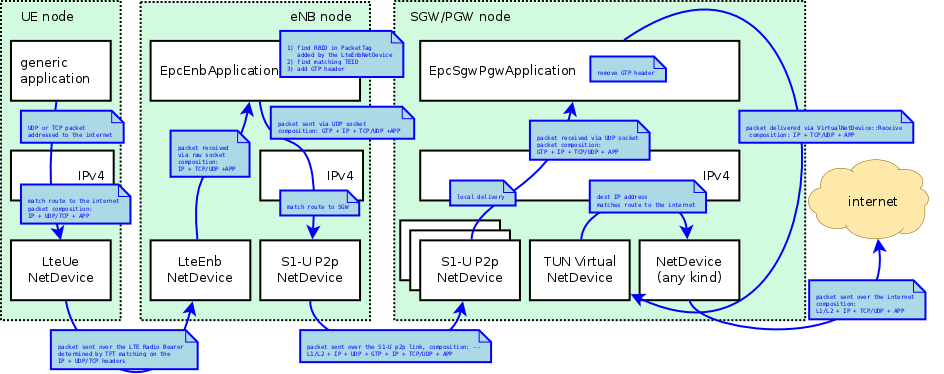
\includegraphics [width=0.95\textwidth] {UploadUE.png}
%  \caption{Поток данных восходящей линии связи между узлом UE и интернетом \cite{LteSimDoc}}
%  \label{img:UploadUE}
%\end{figure}








\section{Анализ эффективности буфера компенсации джиттера в ситуации изменения маршрута передачи пакетов} \label{sect4}



Как уже упоминалось во втором разделе, обновление таблицы маршрутизации может привести к задержке небольшого количества пакетов. Проведем эксперимент для анализа эффективности работы предложенного метода компенсации джиттера. 
На рис. \ref{img4:routeEst} изображен ряд задержек, полученных в сетевом симуляторе NS3 и основные промежуточные величины необходимы для расчета размера буфера: 
оценка задержки (\ref{eq3:playout_d}) и дисперсия оценки (\ref{eq3:playout_v}) для  классического адаптивного буфера \cite{Ramjee} и 
оценка задержки (\ref{eq3:skachok}, \ref{eq3:vibros}) и дисперсия оценки (\ref{eq3:playout_v}) для предложенного метода.






\pgfplotsset{width=15cm, height=10cm, compat=1.3}
\begin{figure} [!ht]
  \center
\begin{tikzpicture}
%\pgfkeys{/pgfplots/legend pos=north west}

\begin{axis}[
mark options={scale=0.25},
ylabel={Mem [GB]},
legend style={
%area legend,
at={(0.5,-0.2)},
anchor=north,
legend columns=2},
legend cell align=left,
%cycle list name=mark list,
cycle list name=linestyles*,
xlabel=Порядковый номер пакета,
ylabel=Задержка (с),
%xmin=380,
%xmax=480
]

				\addplot coordinates {
					(1, 0.025)
					(2, 0.025)
					(3, 0.025)
					(4, 0.025)
					(5, 0.0307430076599)
					(6, 0.030887928009)
					(7, 0.0313809394836)
					(8, 0.0306649303436)
					(9, 0.0304529380798)
					(10, 0.0304281044006)
					(11, 0.0306400203705)
					(12, 0.0303820133209)
					(13, 0.0313771343231)
					(14, 0.0305681419373)
					(15, 0.0312890815735)
					(16, 0.0311550521851)
					(17, 0.0307649612427)
					(18, 0.0306800460815)
					(19, 0.030746049881)
					(20, 0.0329239654541)
					(21, 0.0304090881348)
					(22, 0.0312599658966)
					(23, 0.0315219497681)
					(24, 0.031092042923)
					(25, 0.031308965683)
					(26, 0.0306549453735)
					(27, 0.0314350128174)
					(28, 0.0308811283112)
					(29, 0.0308379364014)
					(30, 0.0304571437836)
					(31, 0.0310879611969)
					(32, 0.0309100627899)
					(33, 0.0326240158081)
					(34, 0.0310821247101)
					(35, 0.0309790897369)
					(36, 0.0312930488586)
					(37, 0.0316749572754)
					(38, 0.0311050987244)
					(39, 0.0315530490875)
					(40, 0.030950050354)
					(41, 0.0311030769348)
					(42, 0.0308410167694)
					(43, 0.0309611415863)
					(44, 0.0310910415649)
					(45, 0.0310979175568)
					(46, 0.0347089672089)
					(47, 0.0415751457214)
					(48, 0.0301219558716)
					(49, 0.0309239578247)
					(50, 0.0314269828796)
					(51, 0.0314131164551)
					(52, 0.0317931175232)
					(53, 0.0328540420532)
					(54, 0.0326239299774)
					(55, 0.0312460708618)
					(56, 0.0323379898071)
					(57, 0.0329370975494)
					(58, 0.0313799476624)
					(59, 0.0322589588165)
					(60, 0.0317289161682)
					(61, 0.0318211460114)
					(62, 0.0463651180267)
					(63, 0.0323749160767)
					(64, 0.0322349262238)
					(65, 0.031990032196)
					(66, 0.0329651260376)
					(67, 0.0315579414368)
					(68, 0.0308641052246)
					(69, 0.0321851444244)
					(70, 0.0318379688263)
					(71, 0.031974067688)
					(72, 0.0321139812469)
					(73, 0.0320359802246)
					(74, 0.032446975708)
					(75, 0.0321279335022)
					(76, 0.0316849136353)
					(77, 0.0304291248322)
					(78, 0.0303201293945)
					(79, 0.0321001243591)
					(80, 0.0317200469971)
					(81, 0.0319429302216)
					(82, 0.0321441173553)
					(83, 0.0318620300293)
					(84, 0.0317001056671)
					(85, 0.0321120548248)
					(86, 0.0323199176788)
					(87, 0.0312329292297)
					(88, 0.0577300167084)
					(89, 0.0311639499664)
					(90, 0.031854133606)
					(91, 0.0343210124969)
					(92, 0.0311590671539)
					(93, 0.0323229885101)
					(94, 0.0315869522095)
					(95, 0.0316801357269)
					(96, 0.0319120788574)
					(97, 0.0308711051941)
					(98, 0.0318600273132)
					(99, 0.0315741252899)
					(100, 0.0309079456329)
					(101, 0.0305600547791)
					(102, 0.0307400226593)
					(103, 0.0307161426544)
					(104, 0.0306989383698)
					(105, 0.0307189273834)
					(106, 0.031064119339)
					(107, 0.0308809757233)
					(108, 0.030800113678)
					(109, 0.0306069564819)
					(110, 0.0311559963226)
					(111, 0.030969991684)
					(112, 0.0305419921875)
					(113, 0.0311599349976)
					(114, 0.0314469528198)
					(115, 0.0309219169617)
					(116, 0.0311629199982)
					(117, 0.0311421394348)
					(118, 0.0312019443512)
					(119, 0.0306721401215)
					(120, 0.0306229877472)
					(121, 0.033869972229)
					(122, 0.0310029506683)
					(123, 0.0310100650787)
					(124, 0.0313841056824)
					(125, 0.0313459205627)
					(126, 0.0316639328003)
					(127, 0.0317599773407)
					(128, 0.0315770721436)
					(129, 0.0321850013733)
					(130, 0.0317069339752)
					(131, 0.0317769908905)
					(132, 0.0321240901947)
					(133, 0.03192902565)
					(134, 0.0310420703888)
					(135, 0.0316881465912)
					(136, 0.0341600322723)
					(137, 0.0323310852051)
					(138, 0.0320530509949)
					(139, 0.0320890140533)
					(140, 0.0342161464691)
					(141, 0.0309879207611)
					(142, 0.0322479248047)
					(143, 0.0320700263977)
					(144, 0.032100982666)
					(145, 0.0318191337585)
					(146, 0.0318231487274)
					(147, 0.0317430019379)
					(148, 0.0320030784607)
					(149, 0.0315741252899)
					(150, 0.0308149623871)
					(151, 0.0310600185394)
					(152, 0.0305991172791)
					(153, 0.0307359313965)
					(154, 0.031720085144)
					(155, 0.0324541378021)
					(156, 0.0318609142303)
					(157, 0.0322599887848)
					(158, 0.032047996521)
					(159, 0.0314149570465)
					(160, 0.031902961731)
					(161, 0.0325271034241)
					(162, 0.0320409297943)
					(163, 0.0318971252441)
					(164, 0.0317311477661)
					(165, 0.0317110824585)
					(166, 0.0342490100861)
					(167, 0.0338529586792)
					(168, 0.0331700897217)
					(169, 0.0317459774017)
					(170, 0.0308671283722)
					(171, 0.0312521362305)
					(172, 0.0320031166077)
					(173, 0.0312899684906)
					(174, 0.0316630554199)
					(175, 0.0302170085907)
					(176, 0.0308819198608)
					(177, 0.0308740139008)
					(178, 0.0318600749969)
					(179, 0.0312771034241)
					(180, 0.0318850326538)
					(181, 0.0301841163635)
					(182, 0.0313060760498)
					(183, 0.0312049484253)
					(184, 0.0310990524292)
					(185, 0.0310220050812)
					(186, 0.0317751312256)
					(187, 0.0321839809418)
					(188, 0.0320520973206)
					(189, 0.0312800598145)
					(190, 0.0305430698395)
					(191, 0.0301739597321)
					(192, 0.0303539276123)
					(193, 0.030755147934)
					(194, 0.0313010883331)
					(195, 0.0316670227051)
					(196, 0.0309331321716)
					(197, 0.0309171199799)
					(198, 0.0318421459198)
					(199, 0.031591053009)
					(200, 0.0310970115662)
					(201, 0.030905046463)
					(202, 0.0307440757751)
					(203, 0.030995092392)
					(204, 0.032368106842)
					(205, 0.0307749557495)
					(206, 0.0303650760651)
					(207, 0.190345096588)
					(208, 0.16714097023)
					(209, 0.170317144394)
					(210, 0.160427980423)
					(211, 0.179161920547)
					(212, 0.153190946579)
					(213, 0.154821929932)
					(214, 0.174789924622)
					(215, 0.180674057007)
					(216, 0.145812931061)
					(217, 0.108640098572)
					(218, 0.083228931427)
					(219, 0.0477970314026)
					(220, 0.0303850460052)
					(221, 0.0321581268311)
					(222, 0.0315579891205)
					(223, 0.031043920517)
					(224, 0.0318311405182)
					(225, 0.0325899887085)
					(226, 0.0336969280243)
					(227, 0.0318920612335)
					(228, 0.0304300403595)
					(229, 0.0309349727631)
					(230, 0.030906085968)
					(231, 0.0316921138763)
					(232, 0.0319400310516)
					(233, 0.0325551128387)
					(234, 0.0319189739227)
					(235, 0.0319151210785)
					(236, 0.0318719291687)
					(237, 0.0318151473999)
					(238, 0.0317979431152)
					(239, 0.0310189914703)
					(240, 0.0316860485077)
					(241, 0.0352610969543)
					(242, 0.0323349475861)
					(243, 0.0318089580536)
					(244, 0.0309069824219)
					(245, 0.0309181499481)
					(246, 0.0313119792938)
					(247, 0.0311030864716)
					(248, 0.0312270259857)
					(249, 0.0309220504761)
					(250, 0.0306409168243)
					(251, 0.0307209873199)
					(252, 0.0307381153107)
					(253, 0.0310179805756)
					(254, 0.0310849380493)
					(255, 0.0312279510498)
					(256, 0.0310629272461)
					(257, 0.0306659221649)
					(258, 0.0305869674683)
					(259, 0.0308370304108)
					(260, 0.0307549762726)
					(261, 0.0309170627594)
					(262, 0.0306230545044)
					(263, 0.0306990718842)
					(264, 0.080240983963)
					(265, 0.0423540878296)
					(266, 0.0306889438629)
					(267, 0.0317269802094)
					(268, 0.0319300746918)
					(269, 0.0320730876923)
					(270, 0.0318880367279)
					(271, 0.0313579940796)
					(272, 0.0319890499115)
					(273, 0.0326630210876)
					(274, 0.0317159843445)
					(275, 0.0310409832001)
					(276, 0.0314901256561)
					(277, 0.0317721366882)
					(278, 0.0323810195923)
					(279, 0.0317799282074)
					(280, 0.0319660949707)
					(281, 0.0316270256042)
					(282, 0.0314491271973)
					(283, 0.0314540958405)
					(284, 0.0314290237427)
					(285, 0.0313851165771)
					(286, 0.0308641338348)
					(287, 0.0315531253815)
					(288, 0.032412109375)
					(289, 0.031754989624)
					(290, 0.0314321327209)
					(291, 0.031500043869)
					(292, 0.0319379806519)
					(293, 0.0310081100464)
					(294, 0.0316141319275)
					(295, 0.0316469955444)
					(296, 0.0334241294861)
					(297, 0.0319249153137)
					(298, 0.0322231388092)
					(299, 0.0322231006622)
					(300, 0.0311361122131)
					(301, 0.0311811351776)
					(302, 0.0306251049042)
					(303, 0.030729970932)
					(304, 0.0307490062714)
					(305, 0.0320569324493)
					(306, 0.0311120414734)
					(307, 0.0323589324951)
					(308, 0.0323779678345)
					(309, 0.032075138092)
					(310, 0.0316619205475)
					(311, 0.0308469676971)
					(312, 0.0323019981384)
					(313, 0.0320430374146)
					(314, 0.0320680332184)
					(315, 0.0310320663452)
					(316, 0.0341729545593)
					(317, 0.032383108139)
					(318, 0.032394990921)
					(319, 0.031699962616)
					(320, 0.0318119812012)
					(321, 0.0308430099487)
					(322, 0.0316280841827)
					(323, 0.0317551231384)
					(324, 0.0317150306702)
					(325, 0.0321169662476)
					(326, 0.0319519424438)
					(327, 0.0322580337524)
					(328, 0.0315539455414)
					(329, 0.0318240356445)
					(330, 0.0323339748383)
					(331, 0.03114112854)
					(332, 0.0332520484924)
					(333, 0.0328631496429)
					(334, 0.0316910457611)
					(335, 0.0322851467133)
					(336, 0.0317751312256)
					(337, 0.0321420192719)
					(338, 0.0318849658966)
					(339, 0.0319240283966)
					(340, 0.0316080856323)
					(341, 0.0322420024872)
					(342, 0.0325800418854)
					(343, 0.0321169948578)
					(344, 0.0315590572357)
					(345, 0.0315919208527)
					(346, 0.0315930747986)
					(347, 0.0304281234741)
					(348, 0.030728969574)
					(349, 0.0303820323944)
					(350, 0.030688123703)
					(351, 0.0308599853516)
					(352, 0.0303890705109)
					(353, 0.0303890323639)
					(354, 0.030424041748)
					(355, 0.0307561206818)
					(356, 0.0305839443207)
					(357, 0.0304549217224)
					(358, 0.0304031467438)
					(359, 0.0308470439911)
					(360, 0.0304009246826)
					(361, 0.0312000656128)
					(362, 0.030762052536)
					(363, 0.0305650806427)
					(364, 0.030409116745)
					(365, 0.0304319667816)
					(366, 0.0305380249023)
					(367, 0.0306149959564)
					(368, 0.0305551147461)
					(369, 0.0309091281891)
					(370, 0.0309551048279)
					(371, 0.0307519340515)
					(372, 0.0302419185638)
					(373, 0.0308999156952)
					(374, 0.0304220867157)
					(375, 0.0306969451904)
					(376, 0.0316131496429)
					(377, 0.0306661128998)
					(378, 0.0305111026764)
					(379, 0.0309910011292)
					(380, 0.0305560874939)
					(381, 0.0305379295349)
					(382, 0.0310709953308)
					(383, 0.030966053009)
					(384, 0.0308201026917)
					(385, 0.0308250713348)
					(386, 0.0309111022949)
					(387, 0.0307911396027)
					(388, 0.0308650112152)
					(389, 0.0305910301208)
					(390, 0.0306670475006)
					(391, 0.0360550308228)
					(392, 0.0325380802155)
					(393, 0.0327440357208)
					(394, 0.0318430137634)
					(395, 0.0312559890747)
					(396, 0.0325620079041)
					(397, 0.032533121109)
					(398, 0.0331350898743)
					(399, 0.0311731052399)
					(400, 0.0316699314117)
					(401, 0.0325580024719)
					(402, 0.0320839881897)
					(403, 0.032368144989)
					(404, 0.0325500202179)
					(405, 0.0309220600128)
					(406, 0.0338891410828)
					(407, 0.0327671051025)
					(408, 0.0326941108704)
					(409, 0.0326950263977)
					(410, 0.0321959781647)
					(411, 0.0320359611511)
					(412, 0.0322609901428)
					(413, 0.032118139267)
					(414, 0.0320160579681)
					(415, 0.0311050224304)
					(416, 0.0309049510956)
					(417, 0.0309161186218)
					(418, 0.0319629764557)
					(419, 0.0321379375458)
					(420, 0.0316860961914)
					(421, 0.031109085083)
					(422, 0.0306889533997)
					(423, 0.0326150989532)
					(424, 0.0317290973663)
					(425, 0.031798915863)
					(426, 0.0316701316833)
					(427, 0.0316369533539)
					(428, 0.0321089839935)
					(429, 0.0317219924927)
					(430, 0.0317789363861)
					(431, 0.0315910243988)
					(432, 0.0313621044159)
					(433, 0.031595954895)
					(434, 0.0317010593414)
					(435, 0.031331949234)
					(436, 0.030958070755)
					(437, 0.031990146637)
					(438, 0.0321291065216)
					(439, 0.0318360519409)
					(440, 0.0315830516815)
					(441, 0.0323449993134)
					(442, 0.0307640075684)
					(443, 0.0321069812775)
					(444, 0.0319550704956)
					(445, 0.0320840167999)
					(446, 0.0318379306793)
					(447, 0.0320851325989)
					(448, 0.0319069957733)
					(449, 0.0318070602417)
					(450, 0.0320690441132)
					(451, 0.0340919876099)
					(452, 0.0319509506226)
					(453, 0.0323059177399)
					(454, 0.0315350723267)
					(455, 0.0321279811859)
					(456, 0.0312240982056)
					(457, 0.0306699752808)
					(458, 0.0305640792847)
					(459, 0.0307399940491)
					(460, 0.0307809638977)
					(461, 0.0308140659332)
					(462, 0.0305539131165)
					(463, 0.0305431461334)
					(464, 0.0303709697723)
					(465, 0.0305919456482)
					(466, 0.0309111499786)
					(467, 0.0305050849915)
					(468, 0.0306891059875)
					(469, 0.0303750705719)
					(470, 0.0304351139069)
					(471, 0.0306029224396)
					(472, 0.0304300308228)
					(473, 0.0306600666046)
					(474, 0.0306669425964)
					(475, 0.0307501125336)
					(476, 0.0314560317993)
					(477, 0.032163143158)
					(478, 0.0321211433411)
					(479, 0.0326539707184)
					(480, 0.0323399353027)
					(481, 0.0318001174927)
					(482, 0.0309091091156)
					(483, 0.030555973053)
					(484, 0.0321111392975)
					(485, 0.0317920970917)
					(486, 0.0310810947418)
					(487, 0.0316129684448)
					(488, 0.0317171192169)
					(489, 0.0315909576416)
					(490, 0.0316340732574)
					(491, 0.0316740894318)
					(492, 0.0316039562225)
					(493, 0.0319579696655)
					(494, 0.0320289802551)
					(495, 0.0321059513092)
					(496, 0.0317790412903)
					(497, 0.0311519622803)
					(498, 0.0307051277161)
					(499, 0.0305570316315)
					(500, 0.0312391090393)
				};
				\addplot coordinates {
					(1, 0.025)
					(2, 0.025)
					(3, 0.025)
					(4, 0.025)
					(5, 0.0251148601532)
					(6, 0.0252303215103)
					(7, 0.0253533338698)
					(8, 0.0254595657993)
					(9, 0.0255594332449)
					(10, 0.025656806668)
					(11, 0.025756470942)
					(12, 0.0258489817896)
					(13, 0.0259595448403)
					(14, 0.0260517167822)
					(15, 0.026156464078)
					(16, 0.0262564358402)
					(17, 0.0263466063482)
					(18, 0.0264332751429)
					(19, 0.0265195306377)
					(20, 0.026647619334)
					(21, 0.02672284871)
					(22, 0.0268135910537)
					(23, 0.026907758228)
					(24, 0.0269914439219)
					(25, 0.0270777943571)
					(26, 0.0271493373775)
					(27, 0.0272350508863)
					(28, 0.0273079724348)
					(29, 0.0273785717141)
					(30, 0.0274401431555)
					(31, 0.0275130995163)
					(32, 0.0275810387818)
					(33, 0.0276818983223)
					(34, 0.0277499028501)
					(35, 0.0278144865878)
					(36, 0.0278840578332)
					(37, 0.0279598758221)
					(38, 0.0280227802801)
					(39, 0.0280933856563)
					(40, 0.0281505189502)
					(41, 0.0282095701099)
					(42, 0.0282621990431)
					(43, 0.028316177894)
					(44, 0.0283716751674)
					(45, 0.0284262000152)
					(46, 0.028551855359)
					(47, 0.0288123211663)
					(48, 0.0288385138604)
					(49, 0.0288802227397)
					(50, 0.0289311579425)
					(51, 0.0289807971127)
					(52, 0.0290370435209)
					(53, 0.0291133834916)
					(54, 0.0291835944213)
					(55, 0.0292248439501)
					(56, 0.0292871068673)
					(57, 0.0293601066809)
					(58, 0.0294005035005)
					(59, 0.0294576726069)
					(60, 0.0295030974781)
					(61, 0.0295494584487)
					(62, 0.0298857716403)
					(63, 0.029935554529)
					(64, 0.0299815419629)
					(65, 0.0300217117676)
					(66, 0.030080580053)
					(67, 0.0301101272807)
					(68, 0.0301252068395)
					(69, 0.0301664055912)
					(70, 0.0301998368559)
					(71, 0.0302353214726)
					(72, 0.0302728946681)
					(73, 0.0303081563792)
					(74, 0.0303509327658)
					(75, 0.0303864727805)
					(76, 0.0304124415976)
					(77, 0.0304127752623)
					(78, 0.0304109223449)
					(79, 0.0304447063852)
					(80, 0.0304702131975)
					(81, 0.0304996675379)
					(82, 0.0305325565343)
					(83, 0.0305591460042)
					(84, 0.0305819651974)
					(85, 0.03061256699)
					(86, 0.0306467140038)
					(87, 0.0306584383083)
					(88, 0.0311998698763)
					(89, 0.0311991514781)
					(90, 0.0312122511207)
					(91, 0.0312744263482)
					(92, 0.0312721191643)
					(93, 0.0312931365512)
					(94, 0.0312990128644)
					(95, 0.0313066353216)
					(96, 0.0313187441923)
					(97, 0.0313097914124)
					(98, 0.0313207961304)
					(99, 0.0313258627136)
					(100, 0.031317504372)
					(101, 0.0313023553801)
					(102, 0.0312911087257)
					(103, 0.0312796094043)
					(104, 0.0312679959836)
					(105, 0.0312570146116)
					(106, 0.0312531567061)
					(107, 0.0312457130865)
					(108, 0.0312368010983)
					(109, 0.031224204206)
					(110, 0.0312228400483)
					(111, 0.031217783081)
					(112, 0.0312042672631)
					(113, 0.0312033806178)
					(114, 0.0312082520619)
					(115, 0.0312025253599)
					(116, 0.0312017332526)
					(117, 0.0312005413763)
					(118, 0.0312005694358)
					(119, 0.0311900008495)
					(120, 0.0311786605874)
					(121, 0.0312324868203)
					(122, 0.0312278960972)
					(123, 0.0312235394769)
					(124, 0.031226750801)
					(125, 0.0312291341962)
					(126, 0.0312378301683)
					(127, 0.0312482731117)
					(128, 0.0312548490924)
					(129, 0.031273452138)
					(130, 0.0312821217747)
					(131, 0.0312920191571)
					(132, 0.0313086605778)
					(133, 0.0313210678793)
					(134, 0.0313154879294)
					(135, 0.0313229411027)
					(136, 0.0313796829261)
					(137, 0.0313987109717)
					(138, 0.0314117977721)
					(139, 0.0314253420977)
					(140, 0.0314811581852)
					(141, 0.0314712934367)
					(142, 0.031486826064)
					(143, 0.0314984900707)
					(144, 0.0315105399226)
					(145, 0.0315167117993)
					(146, 0.0315228405379)
					(147, 0.0315272437659)
					(148, 0.0315367604598)
					(149, 0.0315375077564)
					(150, 0.031523056849)
					(151, 0.0315137960828)
					(152, 0.0314955025068)
					(153, 0.0314803110845)
					(154, 0.0314851065657)
					(155, 0.0315044871905)
					(156, 0.0315116157313)
					(157, 0.0315265831923)
					(158, 0.0315370114589)
					(159, 0.0315345703707)
					(160, 0.0315419381979)
					(161, 0.0315616415024)
					(162, 0.0315712272682)
					(163, 0.0315777452277)
					(164, 0.0315808132785)
					(165, 0.0315834186621)
					(166, 0.0316367304906)
					(167, 0.0316810550544)
					(168, 0.0317108357477)
					(169, 0.0317115385808)
					(170, 0.0316946503766)
					(171, 0.0316858000937)
					(172, 0.031692146424)
					(173, 0.0316841028653)
					(174, 0.0316836819164)
					(175, 0.0316543484499)
					(176, 0.0316388998781)
					(177, 0.0316236021586)
					(178, 0.0316283316153)
					(179, 0.0316213070515)
					(180, 0.0316265815635)
					(181, 0.0315977322595)
					(182, 0.0315918991354)
					(183, 0.0315841601211)
					(184, 0.0315744579673)
					(185, 0.0315634089096)
					(186, 0.0315676433559)
					(187, 0.0315799701076)
					(188, 0.0315894126519)
					(189, 0.0315832255951)
					(190, 0.03156242248)
					(191, 0.0315346532251)
					(192, 0.0315110387128)
					(193, 0.0314959208972)
					(194, 0.0314920242459)
					(195, 0.0314955242151)
					(196, 0.0314842763743)
					(197, 0.0314729332464)
					(198, 0.0314803174998)
					(199, 0.03148253221)
					(200, 0.0314748217971)
					(201, 0.0314634262905)
					(202, 0.0314490392802)
					(203, 0.0314399603424)
					(204, 0.0314585232724)
					(205, 0.0314448519219)
					(206, 0.0314232564048)
					(207, 0.0346016932085)
					(208, 0.0372524787489)
					(209, 0.0399137720618)
					(210, 0.042324056229)
					(211, 0.0450608135154)
					(212, 0.0472234161767)
					(213, 0.0493753864518)
					(214, 0.0518836772152)
					(215, 0.054459484811)
					(216, 0.056286553736)
					(217, 0.0573336246327)
					(218, 0.0578515307686)
					(219, 0.0576504407813)
					(220, 0.0571051328857)
					(221, 0.0566061927647)
					(222, 0.0561052286918)
					(223, 0.0556040025283)
					(224, 0.0551285452881)
					(225, 0.0546777741565)
					(226, 0.0542581572338)
					(227, 0.0538108353138)
					(228, 0.0533432194147)
					(229, 0.0528950544817)
					(230, 0.0524552751114)
					(231, 0.0520400118867)
					(232, 0.05163801227)
					(233, 0.0512563542814)
					(234, 0.0508696066742)
					(235, 0.0504905169623)
					(236, 0.0501181452064)
					(237, 0.0497520852503)
					(238, 0.0493930024076)
					(239, 0.0490255221889)
					(240, 0.0486787327152)
					(241, 0.04841038)
					(242, 0.0480888713517)
					(243, 0.0477632730858)
					(244, 0.0474261472725)
					(245, 0.047095987326)
					(246, 0.0467803071654)
					(247, 0.0464667627515)
					(248, 0.0461619680162)
					(249, 0.0458571696654)
					(250, 0.0455528446086)
					(251, 0.0452562074628)
					(252, 0.0449658456197)
					(253, 0.0446868883189)
					(254, 0.0444148493135)
					(255, 0.0441511113482)
					(256, 0.0438893476662)
					(257, 0.0436248791561)
					(258, 0.0433641209224)
					(259, 0.0431135791121)
					(260, 0.0428664070553)
					(261, 0.0426274201694)
					(262, 0.0423873328561)
					(263, 0.0421535676367)
					(264, 0.0429153159632)
					(265, 0.0429040914005)
					(266, 0.0426597884498)
					(267, 0.042441132285)
					(268, 0.0422309111331)
					(269, 0.0420277546643)
					(270, 0.0418249603056)
					(271, 0.0416156209811)
					(272, 0.0414230895597)
					(273, 0.0412478881902)
					(274, 0.0410572501133)
					(275, 0.040856924775)
					(276, 0.0406695887927)
					(277, 0.0404916397506)
					(278, 0.0403294273474)
					(279, 0.0401584373646)
					(280, 0.0399945905167)
					(281, 0.0398272392185)
					(282, 0.0396596769781)
					(283, 0.0394955653553)
					(284, 0.0393342345231)
					(285, 0.0391752521641)
					(286, 0.0390090297975)
					(287, 0.0388599117092)
					(288, 0.0387309556625)
					(289, 0.0385914363418)
					(290, 0.0384482502694)
					(291, 0.0383092861413)
					(292, 0.0381818600316)
					(293, 0.0380383850319)
					(294, 0.0379098999698)
					(295, 0.0377846418813)
					(296, 0.0376974316334)
					(297, 0.037581981307)
					(298, 0.037474804457)
					(299, 0.0373697703811)
					(300, 0.0372450972178)
					(301, 0.037123817977)
					(302, 0.0369938437155)
					(303, 0.0368685662598)
					(304, 0.0367461750601)
					(305, 0.0366523902078)
					(306, 0.0365415832332)
					(307, 0.0364579302184)
					(308, 0.0363763309707)
					(309, 0.0362903071131)
					(310, 0.0361977393818)
					(311, 0.0360907239481)
					(312, 0.0360149494319)
					(313, 0.0359355111916)
					(314, 0.0358581616321)
					(315, 0.0357616397264)
					(316, 0.035729866023)
					(317, 0.0356629308654)
					(318, 0.0355975720665)
					(319, 0.0355196198775)
					(320, 0.0354454671039)
					(321, 0.0353534179608)
					(322, 0.0352789112853)
					(323, 0.0352084355223)
					(324, 0.0351385674253)
					(325, 0.0350781354017)
					(326, 0.0350156115426)
					(327, 0.0349604599868)
					(328, 0.0348923296979)
					(329, 0.0348309638168)
					(330, 0.0347810240372)
					(331, 0.0347082261273)
					(332, 0.0346791025746)
					(333, 0.034642783516)
					(334, 0.0345837487609)
					(335, 0.0345377767199)
					(336, 0.03448252381)
					(337, 0.0344357137193)
					(338, 0.0343846987628)
					(339, 0.0343354853555)
					(340, 0.034280937361)
					(341, 0.0342401586635)
					(342, 0.034206956328)
					(343, 0.0341651570986)
					(344, 0.0341130351013)
					(345, 0.0340626128163)
					(346, 0.034013222056)
					(347, 0.0339415200844)
					(348, 0.0338772690741)
					(349, 0.0338073643406)
					(350, 0.0337449795278)
					(351, 0.0336872796443)
					(352, 0.0336213154616)
					(353, 0.0335566697997)
					(354, 0.0334940172386)
					(355, 0.0334392593075)
					(356, 0.0333821530077)
					(357, 0.033323608382)
					(358, 0.0332651991493)
					(359, 0.0332168360461)
					(360, 0.0331605178188)
					(361, 0.0331213087747)
					(362, 0.0330741236499)
					(363, 0.0330239427898)
					(364, 0.0329716462689)
					(365, 0.0329208526792)
					(366, 0.0328731961236)
					(367, 0.0328280321203)
					(368, 0.0327825737728)
					(369, 0.0327451048611)
					(370, 0.0327093048605)
					(371, 0.0326701574443)
					(372, 0.0326215926667)
					(373, 0.0325871591272)
					(374, 0.032543857679)
					(375, 0.0325069194292)
					(376, 0.0324890440335)
					(377, 0.0324525854108)
					(378, 0.0324137557561)
					(379, 0.0323853006636)
					(380, 0.0323487164002)
					(381, 0.0323125006629)
					(382, 0.0322876705563)
					(383, 0.0322612382053)
					(384, 0.032232415495)
					(385, 0.0322042686118)
					(386, 0.0321784052855)
					(387, 0.0321506599718)
					(388, 0.0321249469967)
					(389, 0.0320942686592)
					(390, 0.032065724236)
					(391, 0.0321455103678)
					(392, 0.0321533617647)
					(393, 0.0321651752438)
					(394, 0.0321587320142)
					(395, 0.0321406771554)
					(396, 0.0321491037704)
					(397, 0.0321567841172)
					(398, 0.0321763502323)
					(399, 0.0321562853325)
					(400, 0.0321465582541)
					(401, 0.0321547871384)
					(402, 0.0321533711594)
					(403, 0.032157666636)
					(404, 0.0321655137077)
					(405, 0.0321406446338)
					(406, 0.0321756145628)
					(407, 0.0321874443736)
					(408, 0.0321975777035)
					(409, 0.0322075266774)
					(410, 0.0322072957071)
					(411, 0.032203869016)
					(412, 0.0322050114385)
					(413, 0.0322032739951)
					(414, 0.0321995296746)
					(415, 0.0321776395297)
					(416, 0.032152185761)
					(417, 0.0321274644182)
					(418, 0.032124174659)
					(419, 0.0321244499167)
					(420, 0.0321156828422)
					(421, 0.032095550887)
					(422, 0.0320674189373)
					(423, 0.0320783725376)
					(424, 0.0320713870342)
					(425, 0.0320659376107)
					(426, 0.0320580214922)
					(427, 0.0320496001294)
					(428, 0.0320507878067)
					(429, 0.0320442119004)
					(430, 0.0320389063901)
					(431, 0.0320299487503)
					(432, 0.0320165918636)
					(433, 0.0320081791243)
					(434, 0.0320020367286)
					(435, 0.0319886349787)
					(436, 0.0319680236942)
					(437, 0.0319684661531)
					(438, 0.0319716789605)
					(439, 0.0319689664201)
					(440, 0.0319612481253)
					(441, 0.0319689231491)
					(442, 0.0319448248374)
					(443, 0.0319480679662)
					(444, 0.0319482080168)
					(445, 0.0319509241925)
					(446, 0.0319486643222)
					(447, 0.0319513936878)
					(448, 0.0319505057295)
					(449, 0.0319476368197)
					(450, 0.0319500649656)
					(451, 0.0319929034185)
					(452, 0.0319920643626)
					(453, 0.0319983414301)
					(454, 0.031989076048)
					(455, 0.0319918541508)
					(456, 0.0319764990319)
					(457, 0.0319503685569)
					(458, 0.0319226427714)
					(459, 0.031898989797)
					(460, 0.031876629279)
					(461, 0.0318553780121)
					(462, 0.0318293487142)
					(463, 0.0318036246625)
					(464, 0.0317749715647)
					(465, 0.0317513110464)
					(466, 0.0317345078251)
					(467, 0.0317099193684)
					(468, 0.0316895031008)
					(469, 0.0316632144502)
					(470, 0.0316386524393)
					(471, 0.0316179378393)
					(472, 0.031594179699)
					(473, 0.0315754974371)
					(474, 0.0315573263403)
					(475, 0.0315411820642)
					(476, 0.0315394790589)
					(477, 0.0315519523408)
					(478, 0.0315633361608)
					(479, 0.031585148852)
					(480, 0.031600244581)
					(481, 0.0316042420392)
					(482, 0.0315903393808)
					(483, 0.0315696520542)
					(484, 0.0315804817991)
					(485, 0.0315847141049)
					(486, 0.0315746417177)
					(487, 0.0315754082522)
					(488, 0.0315782424715)
					(489, 0.0315784967749)
					(490, 0.0315796083046)
					(491, 0.0315814979271)
					(492, 0.031581947093)
					(493, 0.0315894675445)
					(494, 0.0315982577987)
					(495, 0.0316084116689)
					(496, 0.0316118242613)
					(497, 0.0316026270217)
					(498, 0.0315846770356)
					(499, 0.0315641241275)
					(500, 0.0315576238257)
				};
				\addplot coordinates {
					(1, 0.0)
					(2, 0.0)
					(3, 0.0)
					(4, 0.0)
					(5, 0.000114860153198)
					(6, 0.000228024307251)
					(7, 0.000346476180573)
					(8, 0.000445778586438)
					(9, 0.000536730460321)
					(10, 0.00062336927423)
					(11, 0.000710566162795)
					(12, 0.000788865687117)
					(13, 0.000883651424045)
					(14, 0.000958150337503)
					(15, 0.00104373462658)
					(16, 0.00112283169619)
					(17, 0.00119054557031)
					(18, 0.00125340345357)
					(19, 0.00131459087926)
					(20, 0.00141638775801)
					(21, 0.00146328937886)
					(22, 0.00152476593502)
					(23, 0.0015884377906)
					(24, 0.00164035472869)
					(25, 0.00169389806934)
					(26, 0.00173156312828)
					(27, 0.00178264537451)
					(28, 0.00181991401552)
					(29, 0.00185411501454)
					(30, 0.00187860415564)
					(31, 0.00191398843335)
					(32, 0.00194364793016)
					(33, 0.00200563451208)
					(34, 0.00203352634959)
					(35, 0.00205743956034)
					(36, 0.00208586201455)
					(37, 0.0021199627631)
					(38, 0.00214046796589)
					(39, 0.00216826398272)
					(40, 0.00218203199702)
					(41, 0.00219744251677)
					(42, 0.00220612259962)
					(43, 0.00221597899849)
					(44, 0.00222715669194)
					(45, 0.00223713840589)
					(46, 0.00231805098165)
					(47, 0.00253215576926)
					(48, 0.00250770534798)
					(49, 0.00249926012031)
					(50, 0.0025002101207)
					(51, 0.00249984508854)
					(52, 0.00250609459498)
					(53, 0.00253231267373)
					(54, 0.00255187734997)
					(55, 0.00254208933178)
					(56, 0.00255351046228)
					(57, 0.00257544006668)
					(58, 0.00256432808498)
					(59, 0.0025702106296)
					(60, 0.00256423128823)
					(61, 0.00255930763313)
					(62, 0.00284443467203)
					(63, 0.00283732886732)
					(64, 0.00282656972386)
					(65, 0.00281020813405)
					(66, 0.00281287225677)
					(67, 0.00278616203931)
					(68, 0.0027455183574)
					(69, 0.00273180674195)
					(70, 0.00271060187181)
					(71, 0.00269187445102)
					(72, 0.00267561015749)
					(73, 0.00265735966547)
					(74, 0.00264698885873)
					(75, 0.00262958909629)
					(76, 0.00260296613146)
					(77, 0.00255124047352)
					(78, 0.0025020685814)
					(79, 0.00248581125006)
					(80, 0.00246160183729)
					(81, 0.00244182414103)
					(82, 0.00242587665456)
					(83, 0.00240394859137)
					(84, 0.0023786888128)
					(85, 0.00236171682909)
					(86, 0.00234862950629)
					(87, 0.00231338122068)
					(88, 0.00280854516427)
					(89, 0.00275309265918)
					(90, 0.00271113044855)
					(91, 0.00271908306711)
					(92, 0.00266700858965)
					(93, 0.00263468580477)
					(94, 0.00258786840184)
					(95, 0.00254373349106)
					(96, 0.00250496769195)
					(97, 0.00246382111808)
					(98, 0.00242554941373)
					(99, 0.00238210500865)
					(100, 0.00234282125009)
					(101, 0.00231111381695)
					(102, 0.00227613819502)
					(103, 0.00224211475255)
					(104, 0.00220888587819)
					(105, 0.00217568953263)
					(106, 0.00213603364743)
					(107, 0.00210075659414)
					(108, 0.00206765345042)
					(109, 0.00203889727374)
					(110, 0.00199948348593)
					(111, 0.0019645507835)
					(112, 0.0019387755857)
					(113, 0.0019008867193)
					(114, 0.00186774042895)
					(115, 0.00183611232238)
					(116, 0.00180018218317)
					(117, 0.00176537041586)
					(118, 0.00173009106704)
					(119, 0.00170605783198)
					(120, 0.00168327693739)
					(121, 0.00170343763147)
					(122, 0.00167395960188)
					(123, 0.00164483703022)
					(124, 0.00161515161372)
					(125, 0.00158523197668)
					(126, 0.00156222330923)
					(127, 0.00154142178649)
					(128, 0.0015171693314)
					(129, 0.00150542899039)
					(130, 0.00148399004733)
					(131, 0.0014642076287)
					(132, 0.00145156489688)
					(133, 0.00143494090038)
					(134, 0.00141182203218)
					(135, 0.00139103876477)
					(136, 0.00141995981287)
					(137, 0.00141058866219)
					(138, 0.00139546368942)
					(139, 0.00138109874125)
					(140, 0.00140929285385)
					(141, 0.00139097174526)
					(142, 0.00137868493771)
					(143, 0.00136277524563)
					(144, 0.00134756959263)
					(145, 0.00132679007749)
					(146, 0.0013063830145)
					(147, 0.00128465858221)
					(148, 0.00126848210446)
					(149, 0.00124385975898)
					(150, 0.00123343347118)
					(151, 0.00121802556795)
					(152, 0.00121195863267)
					(153, 0.00120291088222)
					(154, 0.00118364814577)
					(155, 0.00117935580758)
					(156, 0.00116289723222)
					(157, 0.00115460674865)
					(158, 0.00114194288025)
					(159, 0.00112154511089)
					(160, 0.00110648203588)
					(161, 0.00110405569969)
					(162, 0.00109156035153)
					(163, 0.00107624710402)
					(164, 0.00105779021271)
					(165, 0.00103923979205)
					(166, 0.00107176682469)
					(167, 0.00109465605197)
					(168, 0.00110254362428)
					(169, 0.00108119558487)
					(170, 0.00107645987735)
					(171, 0.00106378096272)
					(172, 0.00104885167375)
					(173, 0.00103591819894)
					(174, 0.00101562078387)
					(175, 0.0010246418347)
					(176, 0.00101959756979)
					(177, 0.00101450333794)
					(178, 0.000998942727951)
					(179, 0.000985988437217)
					(180, 0.000971543180519)
					(181, 0.000980961620909)
					(182, 0.000967175512686)
					(183, 0.000955571016633)
					(184, 0.00094616175014)
					(185, 0.00093828757286)
					(186, 0.000923756267722)
					(187, 0.000917607894085)
					(188, 0.000908698280462)
					(189, 0.000896711371601)
					(190, 0.000899580259283)
					(191, 0.000909357909056)
					(192, 0.00091478526313)
					(193, 0.000911607373445)
					(194, 0.000897271877258)
					(195, 0.000882826408895)
					(196, 0.000876417721587)
					(197, 0.000870232495044)
					(198, 0.000860212098611)
					(199, 0.000845222566823)
					(200, 0.000836028528364)
					(201, 0.000830703464479)
					(202, 0.000828476405496)
					(203, 0.00082098581515)
					(204, 0.00082312902884)
					(205, 0.00082033779872)
					(206, 0.000825526559883)
					(207, 0.00398745283235)
					(208, 0.00655848931614)
					(209, 0.00908861284272)
					(210, 0.0113171247531)
					(211, 0.0138275395444)
					(212, 0.0157135914148)
					(213, 0.0175512898616)
					(214, 0.0197085548277)
					(215, 0.021890191327)
					(216, 0.0232794564255)
					(217, 0.0238609381937)
					(218, 0.0239016255657)
					(219, 0.0236246830417)
					(220, 0.0236974972764)
					(221, 0.023722487452)
					(222, 0.0237490017758)
					(223, 0.0237752479038)
					(224, 0.0237752001859)
					(225, 0.0237504673138)
					(226, 0.0236950748901)
					(227, 0.0236684953124)
					(228, 0.0236627413052)
					(229, 0.0236376514121)
					(230, 0.0236046777542)
					(231, 0.0235478474238)
					(232, 0.023478890092)
					(233, 0.0233909702788)
					(234, 0.0233098984804)
					(235, 0.0232227902227)
					(236, 0.0231307061741)
					(237, 0.0230341520068)
					(238, 0.0229325518093)
					(239, 0.0228413809919)
					(240, 0.0227313428457)
					(241, 0.022545068704)
					(242, 0.0224156759782)
					(243, 0.0222929607246)
					(244, 0.0221842273234)
					(245, 0.0220707027234)
					(246, 0.0219449688296)
					(247, 0.0218196138668)
					(248, 0.0216880163248)
					(249, 0.0215590543491)
					(250, 0.021432198319)
					(251, 0.0213001914984)
					(252, 0.0211645495114)
					(253, 0.0210202158221)
					(254, 0.020871850511)
					(255, 0.0207181514661)
					(256, 0.0205655521188)
					(257, 0.0204187095865)
					(258, 0.0202710936285)
					(259, 0.0201162135661)
					(260, 0.0199610613516)
					(261, 0.0198008270105)
					(262, 0.0196448977836)
					(263, 0.0194857650474)
					(264, 0.0198577980729)
					(265, 0.0194718666742)
					(266, 0.0193267322914)
					(267, 0.0191588538104)
					(268, 0.0189858978861)
					(269, 0.0188093363972)
					(270, 0.0186359440279)
					(271, 0.0184725644719)
					(272, 0.0182956446039)
					(273, 0.0181049330812)
					(274, 0.0179334724965)
					(275, 0.0177751283848)
					(276, 0.0176069617995)
					(277, 0.0174327716056)
					(278, 0.0172463285767)
					(279, 0.0170723919879)
					(280, 0.0168947909961)
					(281, 0.0167242464744)
					(282, 0.0165573237853)
					(283, 0.0163902889324)
					(284, 0.016223813986)
					(285, 0.0160583200652)
					(286, 0.0159033760305)
					(287, 0.0157344265982)
					(288, 0.0155486941129)
					(289, 0.0153772395514)
					(290, 0.0152128808328)
					(291, 0.0150475873441)
					(292, 0.0148740617071)
					(293, 0.0147200554726)
					(294, 0.0145541394252)
					(295, 0.0143883147252)
					(296, 0.0141877586786)
					(297, 0.0140194538315)
					(298, 0.0138462416048)
					(299, 0.0136743508486)
					(300, 0.013525536995)
					(301, 0.0133763054959)
					(302, 0.0132387536474)
					(303, 0.0130992560301)
					(304, 0.0129596621093)
					(305, 0.0127942537193)
					(306, 0.0126491756196)
					(307, 0.012479845122)
					(308, 0.0123118474672)
					(309, 0.0121516343755)
					(310, 0.0120011694193)
					(311, 0.0118681614646)
					(312, 0.0117065727515)
					(313, 0.0115518795368)
					(314, 0.0113981915055)
					(315, 0.0112667495812)
					(316, 0.0110731882929)
					(317, 0.0109186596847)
					(318, 0.0107656452899)
					(319, 0.0106282845731)
					(320, 0.0104898716552)
					(321, 0.0103721233652)
					(322, 0.0102391875734)
					(323, 0.0101048795849)
					(324, 0.00997265009025)
					(325, 0.009833629112)
					(326, 0.00969948038891)
					(327, 0.00956064233694)
					(328, 0.00943755977911)
					(329, 0.00931017446459)
					(330, 0.00917391075487)
					(331, 0.00906323044972)
					(332, 0.00891108939342)
					(333, 0.00876918666419)
					(334, 0.008652837686)
					(335, 0.00852575297323)
					(336, 0.00841049082365)
					(337, 0.00828909109794)
					(338, 0.00817432423244)
					(339, 0.00806005115511)
					(340, 0.00795339812647)
					(341, 0.00783510886142)
					(342, 0.00771160901976)
					(343, 0.00759917606877)
					(344, 0.00749931454465)
					(345, 0.00739975053873)
					(346, 0.00730114628831)
					(347, 0.00722682533418)
					(348, 0.0071465398377)
					(349, 0.00707351377454)
					(350, 0.0069944283118)
					(351, 0.00691223962909)
					(352, 0.00683995901918)
					(353, 0.00676780550075)
					(354, 0.00669510195177)
					(355, 0.00661595784387)
					(356, 0.00654074498673)
					(357, 0.0064684747127)
					(358, 0.00639751445121)
					(359, 0.00631792726535)
					(360, 0.00624788694731)
					(361, 0.00616213825249)
					(362, 0.00608608061221)
					(363, 0.00601453986011)
					(364, 0.00594654558381)
					(365, 0.00587840826188)
					(366, 0.00580849665218)
					(367, 0.00573749072248)
					(368, 0.00566819925551)
					(369, 0.00559230418207)
					(370, 0.0055162580991)
					(371, 0.0054450803533)
					(372, 0.00538474352384)
					(373, 0.00531148219279)
					(374, 0.00524855399717)
					(375, 0.00518052116699)
					(376, 0.00509478613938)
					(377, 0.00502934903927)
					(378, 0.00496759171317)
					(379, 0.00489669497145)
					(380, 0.00483534533541)
					(381, 0.00477485416601)
					(382, 0.00470418718933)
					(383, 0.00463653579649)
					(384, 0.00457262779083)
					(385, 0.00450932211822)
					(386, 0.0044449990022)
					(387, 0.00438384433581)
					(388, 0.00432188042423)
					(389, 0.00426612115326)
					(390, 0.00420934315336)
					(391, 0.00420494242203)
					(392, 0.00412869497054)
					(393, 0.00405793455026)
					(394, 0.00398321908886)
					(395, 0.00392160956587)
					(396, 0.00385160398953)
					(397, 0.00378225225651)
					(398, 0.00372617332652)
					(399, 0.00367171475984)
					(400, 0.00360800754306)
					(401, 0.00354407627655)
					(402, 0.00347461073)
					(403, 0.00340941399199)
					(404, 0.00334907278379)
					(405, 0.00330696040201)
					(406, 0.00327579112295)
					(407, 0.00322210511128)
					(408, 0.00316779633899)
					(409, 0.0031143893861)
					(410, 0.00305233256863)
					(411, 0.00299471260838)
					(412, 0.00293596077875)
					(413, 0.0028789790066)
					(414, 0.00282514374701)
					(415, 0.00279053101695)
					(416, 0.0027601741653)
					(417, 0.00272969202477)
					(418, 0.00267838794353)
					(419, 0.00262509544239)
					(420, 0.00258136060805)
					(421, 0.00254986535107)
					(422, 0.0025269999938)
					(423, 0.00248741359424)
					(424, 0.00244465082578)
					(425, 0.00240120723269)
					(426, 0.00236109920658)
					(427, 0.00232229858522)
					(428, 0.0022770402908)
					(429, 0.00223807539126)
					(430, 0.00219861939372)
					(431, 0.00216360464567)
					(432, 0.00213368943945)
					(433, 0.00209942839003)
					(434, 0.00206358221789)
					(435, 0.00203571232342)
					(436, 0.00201560936143)
					(437, 0.00197573963305)
					(438, 0.00193943764776)
					(439, 0.0019033614352)
					(440, 0.00187301250127)
					(441, 0.001843227275)
					(442, 0.00183046104112)
					(443, 0.00179709494909)
					(444, 0.0017612931007)
					(445, 0.00172878341435)
					(446, 0.00169646761632)
					(447, 0.00166526762953)
					(448, 0.00163285023523)
					(449, 0.00160306214028)
					(450, 0.00157342904334)
					(451, 0.00158479891536)
					(452, 0.00155394199297)
					(453, 0.00152914022066)
					(454, 0.00150782279831)
					(455, 0.00148044444511)
					(456, 0.00146619067511)
					(457, 0.00146299733663)
					(458, 0.00146146317534)
					(459, 0.00145588688628)
					(460, 0.00144912966654)
					(461, 0.00144139834012)
					(462, 0.00143859967123)
					(463, 0.00143555172942)
					(464, 0.00143549379264)
					(465, 0.00143044443512)
					(466, 0.00141863876777)
					(467, 0.00141485444909)
					(468, 0.00140697362772)
					(469, 0.00140512280574)
					(470, 0.0014015823605)
					(471, 0.00139426531328)
					(472, 0.00139013814735)
					(473, 0.00138101764629)
					(474, 0.00137156839018)
					(475, 0.00136028129851)
					(476, 0.00133477867783)
					(477, 0.00132055638626)
					(478, 0.00130552907854)
					(479, 0.00130123118812)
					(480, 0.00129030229337)
					(481, 0.00126849370574)
					(482, 0.00125702649009)
					(483, 0.00125257328685)
					(484, 0.00123835156598)
					(485, 0.00121781684051)
					(486, 0.00120353289096)
					(487, 0.00118022876768)
					(488, 0.00115945841162)
					(489, 0.00113652354679)
					(490, 0.00111490460551)
					(491, 0.00109449613594)
					(492, 0.00107305537913)
					(493, 0.001059114723)
					(494, 0.00104672268275)
					(495, 0.00103594209931)
					(496, 0.00101863584975)
					(497, 0.00100746037238)
					(498, 0.00100526115104)
					(499, 0.0010057088361)
					(500, 0.000992094961145)
				};
				\addplot coordinates {
					(1, 0.025)
					(2, 0.025)
					(3, 0.025)
					(4, 0.025)
					(5, 0.025021371169)
					(6, 0.0250503587729)
					(7, 0.0250892662903)
					(8, 0.0251301522423)
					(9, 0.0251753932185)
					(10, 0.0252260464939)
					(11, 0.0252843119603)
					(12, 0.025344739494)
					(13, 0.0254226598558)
					(14, 0.0254944385325)
					(15, 0.025581075141)
					(16, 0.0256698120187)
					(17, 0.0257556912029)
					(18, 0.0258431292623)
					(19, 0.0259344359565)
					(20, 0.0260704165279)
					(21, 0.0261582839879)
					(22, 0.0262654950941)
					(23, 0.0263797877719)
					(24, 0.02648552112)
					(25, 0.0265969397222)
					(26, 0.0266932292879)
					(27, 0.0268085754405)
					(28, 0.0269099486032)
					(29, 0.0270098302374)
					(30, 0.0270992385783)
					(31, 0.027204601562)
					(32, 0.0273041596857)
					(33, 0.0274493646816)
					(34, 0.0275499819995)
					(35, 0.0276462574071)
					(36, 0.0277499436114)
					(37, 0.0278628544634)
					(38, 0.0279571436654)
					(39, 0.0280627791543)
					(40, 0.0281483966502)
					(41, 0.0282367797661)
					(42, 0.0283153131898)
					(43, 0.0283957030965)
					(44, 0.0284781714744)
					(45, 0.0285588490127)
					(46, 0.0287252544691)
					(47, 0.0289092974822)
					(48, 0.0289472768443)
					(49, 0.0290094850515)
					(50, 0.0290859091714)
					(51, 0.0291597870738)
					(52, 0.0292437082681)
					(53, 0.0293591814732)
					(54, 0.0294639522999)
					(55, 0.0295213217985)
					(56, 0.0296122583067)
					(57, 0.0297198905802)
					(58, 0.029773764865)
					(59, 0.0298546053001)
					(60, 0.0299157063241)
					(61, 0.0299779469968)
					(62, 0.0301142196355)
					(63, 0.0301883310717)
					(64, 0.0302555319612)
					(65, 0.0303125704601)
					(66, 0.0303999204573)
					(67, 0.0304381040503)
					(68, 0.0304521675505)
					(69, 0.0305094419787)
					(70, 0.0305533950683)
					(71, 0.0306004421074)
					(72, 0.0306506095011)
					(73, 0.0306965669552)
					(74, 0.0307546789693)
					(75, 0.0308003026391)
					(76, 0.0308297117664)
					(77, 0.0308163858624)
					(78, 0.0307998678762)
					(79, 0.0308431704019)
					(80, 0.0308723876615)
					(81, 0.0309080743643)
					(82, 0.0309492958188)
					(83, 0.0309797472764)
					(84, 0.0310037894707)
					(85, 0.0310407909886)
					(86, 0.0310835107705)
					(87, 0.0310885024826)
					(88, 0.0311433466859)
					(89, 0.0311440353611)
					(90, 0.0311677764521)
					(91, 0.0312732237735)
					(92, 0.0312694054725)
					(93, 0.0313046524165)
					(94, 0.0313140982652)
					(95, 0.0313263480425)
					(96, 0.0313459530884)
					(97, 0.0313300571308)
					(98, 0.0313478007249)
					(99, 0.0313553790937)
					(100, 0.0313403952727)
					(101, 0.0313142601344)
					(102, 0.0312950258763)
					(103, 0.0312756342129)
					(104, 0.0312563141615)
					(105, 0.0312383095751)
					(106, 0.0312324730784)
					(107, 0.0312206948362)
					(108, 0.0312066007769)
					(109, 0.0311865049498)
					(110, 0.0311854824601)
					(111, 0.0311782599644)
					(112, 0.0311569334772)
					(113, 0.0311570340869)
					(114, 0.031166752446)
					(115, 0.0311585450062)
					(116, 0.031158691671)
					(117, 0.0311581367644)
					(118, 0.0311596054403)
					(119, 0.0311436869059)
					(120, 0.0311267115301)
					(121, 0.0311448193537)
					(122, 0.0311400626297)
					(123, 0.0311357038406)
					(124, 0.0311440328649)
					(125, 0.0311508023742)
					(126, 0.0311680084785)
					(127, 0.0311878584814)
					(128, 0.031200909855)
					(129, 0.0312245601373)
					(130, 0.0312407358502)
					(131, 0.0312587186057)
					(132, 0.0312852610548)
					(133, 0.0313068494918)
					(134, 0.0312979701256)
					(135, 0.0313110548079)
					(136, 0.0313372039531)
					(137, 0.0313705345829)
					(138, 0.0313934234983)
					(139, 0.0314167510234)
					(140, 0.0314568437039)
					(141, 0.0314411175825)
					(142, 0.0314681753666)
					(143, 0.0314883596624)
					(144, 0.0315089053125)
					(145, 0.0315193095451)
					(146, 0.0315294995394)
					(147, 0.0315366598937)
					(148, 0.0315523024986)
					(149, 0.0315530343871)
					(150, 0.0315282809996)
					(151, 0.0315125764153)
					(152, 0.0314837437045)
					(153, 0.0314586634551)
					(154, 0.0314674310771)
					(155, 0.0314968412695)
					(156, 0.0315090516822)
					(157, 0.0315342369312)
					(158, 0.0315514676479)
					(159, 0.0315468892826)
					(160, 0.0315588314471)
					(161, 0.0315851020987)
					(162, 0.0316003899517)
					(163, 0.0316103420689)
					(164, 0.0316143937398)
					(165, 0.0316176365608)
					(166, 0.0316392518494)
					(167, 0.0316746113114)
					(168, 0.0317193865084)
					(169, 0.0317202783373)
					(170, 0.0316916646206)
					(171, 0.0316769233097)
					(172, 0.0316878634896)
					(173, 0.0316745185028)
					(174, 0.0316741340427)
					(175, 0.0316434965319)
					(176, 0.0316179540017)
					(177, 0.0315930029745)
					(178, 0.0316019603137)
					(179, 0.0315910649217)
					(180, 0.0316009243239)
					(181, 0.0315717064074)
					(182, 0.031562797409)
					(183, 0.0315507954792)
					(184, 0.0315356444241)
					(185, 0.0315184174192)
					(186, 0.0315270273729)
					(187, 0.031549061018)
					(188, 0.0315659324164)
					(189, 0.0315563444973)
					(190, 0.0315307754191)
					(191, 0.0315020695091)
					(192, 0.0314684717398)
					(193, 0.0314445474645)
					(194, 0.0314397359664)
					(195, 0.0314473589725)
					(196, 0.0314301122362)
					(197, 0.0314129069038)
					(198, 0.0314273032236)
					(199, 0.0314327952558)
					(200, 0.0314215333482)
					(201, 0.0314042108034)
					(202, 0.0313820704168)
					(203, 0.0313690914909)
					(204, 0.0313940241059)
					(205, 0.0313732610583)
					(206, 0.0313448394825)
					(207, 0.0313760095175)
					(208, 0.0323970349051)
					(209, 0.0341389631236)
					(210, 0.158041792547)
					(211, 0.158750144587)
					(212, 0.158563693568)
					(213, 0.15843819783)
					(214, 0.158986621591)
					(215, 0.159714000745)
					(216, 0.159247770029)
					(217, 0.157569018339)
					(218, 0.155783812663)
					(219, 0.153757132154)
					(220, 0.151308869325)
					(221, 0.148395563812)
					(222, 0.0348518235853)
					(223, 0.0347241095579)
					(224, 0.0346270816858)
					(225, 0.0345587592127)
					(226, 0.034529854082)
					(227, 0.0344413846126)
					(228, 0.0343068473228)
					(229, 0.0341937573358)
					(230, 0.034083491456)
					(231, 0.0340032865555)
					(232, 0.0339340866077)
					(233, 0.0338878369245)
					(234, 0.0338218028253)
					(235, 0.0337578542355)
					(236, 0.033694601808)
					(237, 0.0336315664009)
					(238, 0.0335700681329)
					(239, 0.0334845070483)
					(240, 0.0334241881775)
					(241, 0.033485796639)
					(242, 0.0334471980756)
					(243, 0.033392252806)
					(244, 0.0333088988103)
					(245, 0.0332287149912)
					(246, 0.0331644291972)
					(247, 0.0330952933981)
					(248, 0.0330326331916)
					(249, 0.032961845922)
					(250, 0.0328840038015)
					(251, 0.0328114579447)
					(252, 0.0327419196775)
					(253, 0.0326841001275)
					(254, 0.0326304654998)
					(255, 0.0325834262776)
					(256, 0.0325324299459)
					(257, 0.0324698287552)
					(258, 0.0324066790808)
					(259, 0.0323540343091)
					(260, 0.0323004031706)
					(261, 0.0322540070301)
					(262, 0.0321993061755)
					(263, 0.0321489895069)
					(264, 0.0322488534433)
					(265, 0.0325877749929)
					(266, 0.0325240897022)
					(267, 0.0324973552818)
					(268, 0.0324783291405)
					(269, 0.0324647376636)
					(270, 0.0324453955714)
					(271, 0.0324089249874)
					(272, 0.0323948427102)
					(273, 0.0324038372004)
					(274, 0.0323807671608)
					(275, 0.0323358318688)
					(276, 0.0323074675528)
					(277, 0.0322895129799)
					(278, 0.0322925820392)
					(279, 0.032275388036)
					(280, 0.0322650145918)
					(281, 0.0322436169468)
					(282, 0.0322169703904)
					(283, 0.0321913841826)
					(284, 0.0321658152177)
					(285, 0.0321396312041)
					(286, 0.0320968520333)
					(287, 0.0320786158724)
					(288, 0.0320898009801)
					(289, 0.0320785716726)
					(290, 0.0320568906225)
					(291, 0.0320382144238)
					(292, 0.0320348526625)
					(293, 0.0320004165289)
					(294, 0.0319874608496)
					(295, 0.0319760419131)
					(296, 0.0320106241864)
					(297, 0.0320077495787)
					(298, 0.0320149735628)
					(299, 0.0320219539807)
					(300, 0.0319927304928)
					(301, 0.0319655102292)
					(302, 0.0319332190784)
					(303, 0.0318965867881)
					(304, 0.0318580978471)
					(305, 0.0318647666021)
					(306, 0.0318395207979)
					(307, 0.0318569414545)
					(308, 0.0318744162664)
					(309, 0.0318811483173)
					(310, 0.0318737955917)
					(311, 0.0318445053319)
					(312, 0.031859849278)
					(313, 0.0318659932629)
					(314, 0.0318727695229)
					(315, 0.0318468470355)
					(316, 0.0318747836068)
					(317, 0.0318918324088)
					(318, 0.0319087079465)
					(319, 0.0319017067935)
					(320, 0.0318986974683)
					(321, 0.0318696081278)
					(322, 0.0318615076061)
					(323, 0.0318579395554)
					(324, 0.0318531465047)
					(325, 0.0318619948098)
					(326, 0.0318650115821)
					(327, 0.0318781932342)
					(328, 0.0318673182236)
					(329, 0.0318658665602)
					(330, 0.0318815665408)
					(331, 0.0318632146456)
					(332, 0.0318839002914)
					(333, 0.0319106804431)
					(334, 0.0319033140699)
					(335, 0.0319161204341)
					(336, 0.0319113917678)
					(337, 0.0319191268315)
					(338, 0.0319179811008)
					(339, 0.0319181839223)
					(340, 0.0319077834715)
					(341, 0.0319189929124)
					(342, 0.0319360112459)
					(343, 0.0319420812928)
					(344, 0.0319292349695)
					(345, 0.0319179217213)
					(346, 0.031907026613)
					(347, 0.031889410325)
					(348, 0.0318647529285)
					(349, 0.0318359249518)
					(350, 0.030722615186)
					(351, 0.0307272224724)
					(352, 0.0307158811236)
					(353, 0.0307049188753)
					(354, 0.030695498479)
					(355, 0.0306975316997)
					(356, 0.030693722069)
					(357, 0.0306857128946)
					(358, 0.0306762358499)
					(359, 0.0306819646196)
					(360, 0.0306725387628)
					(361, 0.0306902315953)
					(362, 0.0306926404127)
					(363, 0.0306883621591)
					(364, 0.0306789964893)
					(365, 0.0306707113086)
					(366, 0.0306662611117)
					(367, 0.0306645417191)
					(368, 0.0306608716251)
					(369, 0.0306691979535)
					(370, 0.0306787870435)
					(371, 0.0306812403362)
					(372, 0.0306701498326)
					(373, 0.0306778559975)
					(374, 0.0306692776985)
					(375, 0.0306702056443)
					(376, 0.0306812172649)
					(377, 0.0306807106765)
					(378, 0.0306750221586)
					(379, 0.0306856198428)
					(380, 0.0306812754305)
					(381, 0.0306764677228)
					(382, 0.0306883142522)
					(383, 0.03069762939)
					(384, 0.0307017370475)
					(385, 0.0307058735818)
					(386, 0.0307127567901)
					(387, 0.0307153856875)
					(388, 0.0307204040092)
					(389, 0.0307160649115)
					(390, 0.0307144209064)
					(391, 0.0307230604269)
					(392, 0.0307639988194)
					(393, 0.0308111637865)
					(394, 0.030845771217)
					(395, 0.0308595295988)
					(396, 0.0309088080191)
					(397, 0.0309625671263)
					(398, 0.0310197583019)
					(399, 0.0310249014367)
					(400, 0.0310465352308)
					(401, 0.0310972286442)
					(402, 0.0311303237773)
					(403, 0.0311718393197)
					(404, 0.0312180624148)
					(405, 0.0312081347288)
					(406, 0.0312605952986)
					(407, 0.0313111224435)
					(408, 0.0313575067792)
					(409, 0.0314023661272)
					(410, 0.0314289832459)
					(411, 0.0314493408038)
					(412, 0.0314765628794)
					(413, 0.031498080843)
					(414, 0.0315154533852)
					(415, 0.0315016878563)
					(416, 0.0314816737783)
					(417, 0.0314627055065)
					(418, 0.0314794841977)
					(419, 0.0315015682011)
					(420, 0.0315077571237)
					(421, 0.0314943859794)
					(422, 0.031467372409)
					(423, 0.0315015530427)
					(424, 0.0315091846989)
					(425, 0.0315189020526)
					(426, 0.0315239741745)
					(427, 0.0315277634067)
					(428, 0.0315472570845)
					(429, 0.0315531175716)
					(430, 0.0315606913557)
					(431, 0.0315617087019)
					(432, 0.0315550141323)
					(433, 0.0315563872531)
					(434, 0.0315612394403)
					(435, 0.0315535492285)
					(436, 0.0315387422796)
					(437, 0.031553882024)
					(438, 0.0315712963944)
					(439, 0.0315801760856)
					(440, 0.0315802725308)
					(441, 0.0315961571919)
					(442, 0.031577478571)
					(443, 0.0315952376721)
					(444, 0.0316073061798)
					(445, 0.0316232946762)
					(446, 0.0316304933977)
					(447, 0.0316457416362)
					(448, 0.0316545038929)
					(449, 0.0316596205119)
					(450, 0.031673352255)
					(451, 0.0316919255627)
					(452, 0.0317006130579)
					(453, 0.0317209144972)
					(454, 0.0317146814981)
					(455, 0.031728543242)
					(456, 0.0317116245553)
					(457, 0.0316857498796)
					(458, 0.0316565992305)
					(459, 0.0316258570191)
					(460, 0.0315975199734)
					(461, 0.0315712435459)
					(462, 0.0315371230895)
					(463, 0.0315037858902)
					(464, 0.0314657921354)
					(465, 0.0314364840168)
					(466, 0.0314188647295)
					(467, 0.0313882172813)
					(468, 0.0313647696426)
					(469, 0.0313315759201)
					(470, 0.0313015092947)
					(471, 0.0312780792452)
					(472, 0.0312496363733)
					(473, 0.0312298626705)
					(474, 0.0312109827773)
					(475, 0.0311955255546)
					(476, 0.0312042627276)
					(477, 0.0312364228173)
					(478, 0.0312660956425)
					(479, 0.031302331441)
					(480, 0.0313371318521)
					(481, 0.0313526600236)
					(482, 0.0313377836777)
					(483, 0.0313115623689)
					(484, 0.0313383795454)
					(485, 0.0313535968723)
					(486, 0.0313444573668)
					(487, 0.0313534630156)
					(488, 0.0313656597564)
					(489, 0.0313732160689)
					(490, 0.0313819650122)
					(491, 0.0313917626338)
					(492, 0.0313988794385)
					(493, 0.0314176308817)
					(494, 0.0314381350551)
					(495, 0.031460533083)
					(496, 0.0314712155959)
					(497, 0.0314605080927)
					(498, 0.0314375854021)
					(499, 0.0314128069205)
					(500, 0.0314069812312)
				};
				\addplot coordinates {
					(1, 0.0)
					(2, 0.0)
					(3, 0.0)
					(4, 0.0)
					(5, 0.000114860153198)
					(6, 0.000229894086935)
					(7, 0.00035190781941)
					(8, 0.000456382944089)
					(9, 0.000553711001958)
					(10, 0.000647691005561)
					(11, 0.000743016662982)
					(12, 0.000830110356935)
					(13, 0.000934156046378)
					(14, 0.00101838256708)
					(15, 0.00111390777656)
					(16, 0.00120310916191)
					(17, 0.00128094996315)
					(18, 0.00135381806146)
					(19, 0.0014248001126)
					(20, 0.0015360947003)
					(21, 0.00159214623843)
					(22, 0.00166233695184)
					(23, 0.00173421930628)
					(24, 0.00179378002318)
					(25, 0.00185437331397)
					(26, 0.00189844596072)
					(27, 0.0019553127121)
					(28, 0.00199765751527)
					(29, 0.00203626412093)
					(30, 0.00206448510943)
					(31, 0.00210296985961)
					(32, 0.00213501968698)
					(33, 0.00219871641569)
					(34, 0.00222739728795)
					(35, 0.00225143149693)
					(36, 0.00227933869603)
					(37, 0.00231225219539)
					(38, 0.0023308520367)
					(39, 0.00235615310441)
					(40, 0.00236677546631)
					(41, 0.00237853356268)
					(42, 0.00238304763149)
					(43, 0.00238830324679)
					(44, 0.00239444395122)
					(45, 0.00239894999385)
					(46, 0.00247397335789)
					(47, 0.00268149171578)
					(48, 0.00265211504925)
					(49, 0.00263860636788)
					(50, 0.00263418419708)
					(51, 0.00262804465881)
					(52, 0.00262815037463)
					(53, 0.00264779404284)
					(54, 0.00266013313206)
					(55, 0.00264257284066)
					(56, 0.00264605474402)
					(57, 0.00265963043399)
					(58, 0.00263963896696)
					(59, 0.00263655006665)
					(60, 0.00262130528268)
					(61, 0.00260698797077)
					(62, 0.00288259163195)
					(63, 0.00287015372814)
					(64, 0.00285368255661)
					(65, 0.00283129891018)
					(66, 0.00282772404353)
					(67, 0.00279432998225)
					(68, 0.00274696340609)
					(69, 0.00272668367544)
					(70, 0.00269872053889)
					(71, 0.0026731595805)
					(72, 0.00264996717168)
					(73, 0.00262467524272)
					(74, 0.00260718991292)
					(75, 0.00258251120532)
					(76, 0.00254855320114)
					(77, 0.0025055938758)
					(78, 0.00246540712764)
					(79, 0.00244210411474)
					(80, 0.00241079956435)
					(81, 0.00238399442427)
					(82, 0.0023610353956)
					(83, 0.0023320693719)
					(84, 0.00229983515227)
					(85, 0.00227600375631)
					(86, 0.00225606621499)
					(87, 0.00221393325987)
					(88, 0.00270248487919)
					(89, 0.00264884724722)
					(90, 0.00261007226717)
					(91, 0.00262093554273)
					(92, 0.00257079996426)
					(93, 0.00254045562573)
					(94, 0.00249529250908)
					(95, 0.00245270740813)
					(96, 0.00241536787627)
					(97, 0.00237655747663)
					(98, 0.00233962573074)
					(99, 0.00229735970743)
					(100, 0.00226036118249)
					(101, 0.00223076076872)
					(102, 0.00219763030285)
					(103, 0.00216525536123)
					(104, 0.00213348417086)
					(105, 0.00210156222301)
					(106, 0.00206301478327)
					(107, 0.00202878443471)
					(108, 0.00199662036918)
					(109, 0.00196868084769)
					(110, 0.00192991740328)
					(111, 0.00189562887074)
					(112, 0.00187044164886)
					(113, 0.00183309284629)
					(114, 0.00180222936402)
					(115, 0.00177108148643)
					(116, 0.00173574735654)
					(117, 0.00170136345414)
					(118, 0.00166821233679)
					(119, 0.00164459739643)
					(120, 0.00162211943168)
					(121, 0.00164454225702)
					(122, 0.00161448878559)
					(123, 0.0015847989609)
					(124, 0.00155807101852)
					(125, 0.0015309473521)
					(126, 0.00151059101358)
					(127, 0.00149221857055)
					(128, 0.00147015847239)
					(129, 0.00146043713331)
					(130, 0.0014408758674)
					(131, 0.00142278345086)
					(132, 0.00141163521362)
					(133, 0.00139627780125)
					(134, 0.00137364782729)
					(135, 0.00135397840005)
					(136, 0.00138387838134)
					(137, 0.00137607843875)
					(138, 0.00136220719822)
					(139, 0.00134887486535)
					(140, 0.00137788527696)
					(141, 0.00135970603028)
					(142, 0.00134864805412)
					(143, 0.00133371211366)
					(144, 0.00131929033146)
					(145, 0.00129910909375)
					(146, 0.00127920369552)
					(147, 0.00125788966958)
					(148, 0.00124206024753)
					(149, 0.0012176554984)
					(150, 0.00120806382843)
					(151, 0.00119326780107)
					(152, 0.00118767162777)
					(153, 0.00117887444138)
					(154, 0.00116052538633)
					(155, 0.00115704901311)
					(156, 0.00114118949206)
					(157, 0.00113338444427)
					(158, 0.00112099194718)
					(159, 0.00110130232026)
					(160, 0.00108639772283)
					(161, 0.00108403520791)
					(162, 0.00107147105766)
					(163, 0.00105597634236)
					(164, 0.00103727292945)
					(165, 0.00101846124524)
					(166, 0.00105071949084)
					(167, 0.00107397923762)
					(168, 0.00108240922107)
					(169, 0.00106129285452)
					(170, 0.00105712999673)
					(171, 0.00104477796459)
					(172, 0.00103040627126)
					(173, 0.00101775604582)
					(174, 0.000997630186557)
					(175, 0.00100682009187)
					(176, 0.00100191522345)
					(177, 0.000996755721)
					(178, 0.000982162047029)
					(179, 0.000969015943881)
					(180, 0.000955514979646)
					(181, 0.00096474083926)
					(182, 0.000950758629628)
					(183, 0.000938900436709)
					(184, 0.000929157288976)
					(185, 0.000920846930056)
					(186, 0.000907564267582)
					(187, 0.000902552053608)
					(188, 0.000894561738588)
					(189, 0.000882387955855)
					(190, 0.000885005689893)
					(191, 0.000894441889836)
					(192, 0.000899515889975)
					(193, 0.000895792048291)
					(194, 0.000880745389953)
					(195, 0.000867676216928)
					(196, 0.000860607228607)
					(197, 0.000853654929161)
					(198, 0.000845166610897)
					(199, 0.000831538274387)
					(200, 0.000821623182691)
					(201, 0.00081552045674)
					(202, 0.000812412748171)
					(203, 0.000803904053704)
					(204, 0.000807806279652)
					(205, 0.000804031521188)
					(206, 0.000808114590628)
					(207, 0.00397195744093)
					(208, 0.00660781750636)
					(209, 0.00923406334601)
					(210, 0.0115751624251)
					(211, 0.0117660617366)
					(212, 0.011641924462)
					(213, 0.0114839212455)
					(214, 0.0115812773564)
					(215, 0.0117834005176)
					(216, 0.0118257539009)
					(217, 0.0126013922521)
					(218, 0.0138361661453)
					(219, 0.0157191784476)
					(220, 0.0178722366016)
					(221, 0.0198978067194)
					(222, 0.0218366020789)
					(223, 0.0214760280987)
					(224, 0.0211043669175)
					(225, 0.0207230214387)
					(226, 0.0203257976337)
					(227, 0.019972037538)
					(228, 0.0196528236723)
					(229, 0.01932720469)
					(230, 0.0190064140236)
					(231, 0.0186741132947)
					(232, 0.0183418961389)
					(233, 0.0180026376915)
					(234, 0.0176819621977)
					(235, 0.0173664565887)
					(236, 0.0170568459582)
					(237, 0.0167532981272)
					(238, 0.0164549046304)
					(239, 0.016176828071)
					(240, 0.0158892606804)
					(241, 0.0156082136424)
					(242, 0.0153190663506)
					(243, 0.015045449824)
					(244, 0.0147942462352)
					(245, 0.0145461762877)
					(246, 0.0142935874759)
					(247, 0.0140489425809)
					(248, 0.0138053290776)
					(249, 0.0135714341503)
					(250, 0.0133464240493)
					(251, 0.0131227558979)
					(252, 0.0129017676326)
					(253, 0.012678211062)
					(254, 0.0124566300823)
					(255, 0.0122355477697)
					(256, 0.0120212467949)
					(257, 0.0118181520147)
					(258, 0.0116194462001)
					(259, 0.0114184502495)
					(260, 0.0112220624052)
					(261, 0.0110252879654)
					(262, 0.0108374012566)
					(263, 0.0106506579173)
					(264, 0.011399484648)
					(265, 0.0113735996428)
					(266, 0.0111841042725)
					(267, 0.010976364377)
					(268, 0.0107681827012)
					(269, 0.0105609238762)
					(270, 0.0103612394173)
					(271, 0.0101757626588)
					(272, 0.00998064490718)
					(273, 0.00978639557658)
					(274, 0.00960442472217)
					(275, 0.00943913190694)
					(276, 0.00926726339305)
					(277, 0.00909262474249)
					(278, 0.00891260237988)
					(279, 0.00874460340892)
					(280, 0.00857589720205)
					(281, 0.00841713903776)
					(282, 0.00826468605199)
					(283, 0.00811464982195)
					(284, 0.00796760403431)
					(285, 0.00782386592644)
					(286, 0.00769289855529)
					(287, 0.00754991511722)
					(288, 0.00740558668493)
					(289, 0.00726417117836)
					(290, 0.00713181653382)
					(291, 0.00700031713822)
					(292, 0.00686231547089)
					(293, 0.00674560401379)
					(294, 0.00661841762555)
					(295, 0.00649285857914)
					(296, 0.00639196315902)
					(297, 0.00626583807329)
					(298, 0.00614482909643)
					(299, 0.00602609505649)
					(300, 0.00592328999072)
					(301, 0.00582105609721)
					(302, 0.00573144308176)
					(303, 0.00564087918305)
					(304, 0.00555101320973)
					(305, 0.00544396963758)
					(306, 0.0053501447474)
					(307, 0.0052535300864)
					(308, 0.00515888001227)
					(309, 0.00505971684854)
					(310, 0.00496290706696)
					(311, 0.00488418548351)
					(312, 0.00479565162998)
					(313, 0.00470340236011)
					(314, 0.00461337511201)
					(315, 0.00453792167333)
					(316, 0.00449368539034)
					(317, 0.00441397817317)
					(318, 0.00433576177996)
					(319, 0.00425322145097)
					(320, 0.0041699515338)
					(321, 0.00410766625351)
					(322, 0.00403034340734)
					(323, 0.00395186422855)
					(324, 0.00387568512168)
					(325, 0.00380344781411)
					(326, 0.00372917781051)
					(327, 0.0036624546977)
					(328, 0.00359569055761)
					(329, 0.00352464239804)
					(330, 0.00346351171564)
					(331, 0.00340905024134)
					(332, 0.00336864591345)
					(333, 0.00332085798221)
					(334, 0.00325883351621)
					(335, 0.00320129349875)
					(336, 0.00314008741294)
					(337, 0.00308189821477)
					(338, 0.00302094346917)
					(339, 0.0029606455457)
					(340, 0.00290763460059)
					(341, 0.00285616628889)
					(342, 0.00281226394257)
					(343, 0.00275963833596)
					(344, 0.00271210605038)
					(345, 0.00266461021171)
					(346, 0.00261781494593)
					(347, 0.00259503670979)
					(348, 0.00256634479062)
					(349, 0.00254467230548)
					(350, 0.00251673488435)
					(351, 0.00246914758998)
					(352, 0.00242652767741)
					(353, 0.00238453409905)
					(354, 0.00234246095962)
					(355, 0.00229682418448)
					(356, 0.00225315944837)
					(357, 0.00221287226633)
					(358, 0.00217426614403)
					(359, 0.00213419698397)
					(360, 0.00209713384303)
					(361, 0.00206574170317)
					(362, 0.00202586328792)
					(363, 0.00198789721756)
					(364, 0.00195372418149)
					(365, 0.00191959029201)
					(366, 0.0018838522143)
					(367, 0.00184720047312)
					(368, 0.00181244500312)
					(369, 0.00178116123433)
					(370, 0.00175125614714)
					(371, 0.00171769396435)
					(372, 0.00169212652051)
					(373, 0.00166287930735)
					(374, 0.00163473710684)
					(375, 0.00160259571454)
					(376, 0.00158940268023)
					(377, 0.00155791671392)
					(378, 0.00153015053965)
					(379, 0.00150586710827)
					(380, 0.00147834041308)
					(381, 0.00145164052273)
					(382, 0.00143049826444)
					(383, 0.00140744307428)
					(384, 0.00138174367883)
					(385, 0.001356575491)
					(386, 0.00133354855544)
					(387, 0.00130844524058)
					(388, 0.00128526884633)
					(389, 0.00126215094717)
					(390, 0.00123788827644)
					(391, 0.00131994270924)
					(392, 0.00132984425082)
					(393, 0.00134284810384)
					(394, 0.0013366281413)
					(395, 0.00131809993563)
					(396, 0.00132578750302)
					(397, 0.00133175801476)
					(398, 0.00134857330942)
					(399, 0.00132466878199)
					(400, 0.00131107600585)
					(401, 0.00131508383056)
					(402, 0.00130851734486)
					(403, 0.00130710342219)
					(404, 0.00130852497171)
					(405, 0.00128827452032)
					(406, 0.00131612915699)
					(407, 0.00131993676993)
					(408, 0.00132119780307)
					(409, 0.00132152423938)
					(410, 0.00131096599534)
					(411, 0.00129688623354)
					(412, 0.00128718149565)
					(413, 0.00127426939349)
					(414, 0.00125914354812)
					(415, 0.00124216929625)
					(416, 0.00122926064554)
					(417, 0.00121598653576)
					(418, 0.00120167222403)
					(419, 0.00119080784651)
					(420, 0.00117068224938)
					(421, 0.00115524204521)
					(422, 0.0011482458559)
					(423, 0.00114823546967)
					(424, 0.00112982164675)
					(425, 0.00111301983709)
					(426, 0.00109378403297)
					(427, 0.0010741679359)
					(428, 0.00106430898891)
					(429, 0.0010465175173)
					(430, 0.00103010354324)
					(431, 0.00101010813324)
					(432, 0.000993898056297)
					(433, 0.000974838910424)
					(434, 0.000958235573983)
					(435, 0.000943656666628)
					(436, 0.000936693102765)
					(437, 0.000926987327857)
					(438, 0.000919952071252)
					(439, 0.000906848140758)
					(440, 0.000888768689862)
					(441, 0.000886287851717)
					(442, 0.000885205087152)
					(443, 0.000878091039538)
					(444, 0.000867725875217)
					(445, 0.000859905570114)
					(446, 0.000847000178774)
					(447, 0.000839152959223)
					(448, 0.000827594982782)
					(449, 0.000814094210103)
					(450, 0.000806000797926)
					(451, 0.000838253489065)
					(452, 0.000826668920482)
					(453, 0.000822241635712)
					(454, 0.000809513646408)
					(455, 0.000801589367237)
					(456, 0.000795646480622)
					(457, 0.0008005665365)
					(458, 0.00080698861767)
					(459, 0.000809180948944)
					(460, 0.000809895192394)
					(461, 0.00080936636935)
					(462, 0.000813525650551)
					(463, 0.000817134676663)
					(464, 0.000823448305486)
					(465, 0.000824456269121)
					(466, 0.000818473824502)
					(467, 0.000820379942773)
					(468, 0.000817954569792)
					(469, 0.00082138945981)
					(470, 0.000822890910879)
					(471, 0.000820404829764)
					(472, 0.000820957701618)
					(473, 0.000816329942959)
					(474, 0.00081126174558)
					(475, 0.000804253915544)
					(476, 0.000793378962127)
					(477, 0.000796688991492)
					(478, 0.000798449622138)
					(479, 0.000810238131213)
					(480, 0.000814785445824)
					(481, 0.000807749449719)
					(482, 0.000800465478884)
					(483, 0.0008000923818)
					(484, 0.000800082072735)
					(485, 0.000793154782206)
					(486, 0.000782741729172)
					(487, 0.000772457116148)
					(488, 0.000764281097852)
					(489, 0.000753501433599)
					(490, 0.000743648548699)
					(491, 0.000734618066115)
					(492, 0.000724169576568)
					(493, 0.000720867989577)
					(494, 0.000718677617254)
					(495, 0.000717660389991)
					(496, 0.000709677346337)
					(497, 0.000701868865721)
					(498, 0.000702939095939)
					(499, 0.000706491389433)
					(500, 0.000695835519269)
				};


\legend{Задержка, Оценка задержки \cite{Ramjee}, Дисперсия оценки \cite{Ramjee}, Оценка задержки ГРФК, Дисперсия оценки ГРФК}
\end{axis}
\end{tikzpicture}
\caption{Основные промежуточные величины, необходимые для расчета размера буфера}
  \label{img4:routeEst}
\end{figure}


Оценка задержки используется как время отправки первого пакета речевой активности.
Дисперсия оценки используется для расчета времени задержки буфера на основе (\ref{eq41:syntes3}-\ref{eq41:syntes5}).
Как можно увидеть на рис. \ref{img4:routeBuff}, размер классического буфера компенсации джиттера значительное время остается завышенным (в данном случае на протяжении 3 интервалов речевой активности),
в то время как предложенный метод менее инерционен и быстрее адаптируется к изменениям сетевой ситуации.

\pgfplotsset{width=15cm, height=10cm, compat=1.3}
\begin{figure} [!ht]
  \center
\begin{tikzpicture}
%\pgfkeys{/pgfplots/legend pos=north west}

\begin{axis}[
%mark options={scale=0.5},
ylabel={Mem [GB]},
legend style={
%area legend,
at={(0.5,-0.2)},
anchor=north,
legend columns=1},
legend cell align=left,
%cycle list name=mark list,
cycle list name=linestyles,
xlabel=Порядковый номер пакета,
ylabel=Задержка/Задержка воспроизведения (с),
%xmin=380,
%xmax=480
]

				\addplot coordinates {
					(1, 0.025)
					(2, 0.025)
					(3, 0.025)
					(4, 0.025)
					(5, 0.0307430076599)
					(6, 0.030887928009)
					(7, 0.0313809394836)
					(8, 0.0306649303436)
					(9, 0.0304529380798)
					(10, 0.0304281044006)
					(11, 0.0306400203705)
					(12, 0.0303820133209)
					(13, 0.0313771343231)
					(14, 0.0305681419373)
					(15, 0.0312890815735)
					(16, 0.0311550521851)
					(17, 0.0307649612427)
					(18, 0.0306800460815)
					(19, 0.030746049881)
					(20, 0.0329239654541)
					(21, 0.0304090881348)
					(22, 0.0312599658966)
					(23, 0.0315219497681)
					(24, 0.031092042923)
					(25, 0.031308965683)
					(26, 0.0306549453735)
					(27, 0.0314350128174)
					(28, 0.0308811283112)
					(29, 0.0308379364014)
					(30, 0.0304571437836)
					(31, 0.0310879611969)
					(32, 0.0309100627899)
					(33, 0.0326240158081)
					(34, 0.0310821247101)
					(35, 0.0309790897369)
					(36, 0.0312930488586)
					(37, 0.0316749572754)
					(38, 0.0311050987244)
					(39, 0.0315530490875)
					(40, 0.030950050354)
					(41, 0.0311030769348)
					(42, 0.0308410167694)
					(43, 0.0309611415863)
					(44, 0.0310910415649)
					(45, 0.0310979175568)
					(46, 0.0347089672089)
					(47, 0.0415751457214)
					(48, 0.0301219558716)
					(49, 0.0309239578247)
					(50, 0.0314269828796)
					(51, 0.0314131164551)
					(52, 0.0317931175232)
					(53, 0.0328540420532)
					(54, 0.0326239299774)
					(55, 0.0312460708618)
					(56, 0.0323379898071)
					(57, 0.0329370975494)
					(58, 0.0313799476624)
					(59, 0.0322589588165)
					(60, 0.0317289161682)
					(61, 0.0318211460114)
					(62, 0.0463651180267)
					(63, 0.0323749160767)
					(64, 0.0322349262238)
					(65, 0.031990032196)
					(66, 0.0329651260376)
					(67, 0.0315579414368)
					(68, 0.0308641052246)
					(69, 0.0321851444244)
					(70, 0.0318379688263)
					(71, 0.031974067688)
					(72, 0.0321139812469)
					(73, 0.0320359802246)
					(74, 0.032446975708)
					(75, 0.0321279335022)
					(76, 0.0316849136353)
					(77, 0.0304291248322)
					(78, 0.0303201293945)
					(79, 0.0321001243591)
					(80, 0.0317200469971)
					(81, 0.0319429302216)
					(82, 0.0321441173553)
					(83, 0.0318620300293)
					(84, 0.0317001056671)
					(85, 0.0321120548248)
					(86, 0.0323199176788)
					(87, 0.0312329292297)
					(88, 0.0577300167084)
					(89, 0.0311639499664)
					(90, 0.031854133606)
					(91, 0.0343210124969)
					(92, 0.0311590671539)
					(93, 0.0323229885101)
					(94, 0.0315869522095)
					(95, 0.0316801357269)
					(96, 0.0319120788574)
					(97, 0.0308711051941)
					(98, 0.0318600273132)
					(99, 0.0315741252899)
					(100, 0.0309079456329)
					(101, 0.0305600547791)
					(102, 0.0307400226593)
					(103, 0.0307161426544)
					(104, 0.0306989383698)
					(105, 0.0307189273834)
					(106, 0.031064119339)
					(107, 0.0308809757233)
					(108, 0.030800113678)
					(109, 0.0306069564819)
					(110, 0.0311559963226)
					(111, 0.030969991684)
					(112, 0.0305419921875)
					(113, 0.0311599349976)
					(114, 0.0314469528198)
					(115, 0.0309219169617)
					(116, 0.0311629199982)
					(117, 0.0311421394348)
					(118, 0.0312019443512)
					(119, 0.0306721401215)
					(120, 0.0306229877472)
					(121, 0.033869972229)
					(122, 0.0310029506683)
					(123, 0.0310100650787)
					(124, 0.0313841056824)
					(125, 0.0313459205627)
					(126, 0.0316639328003)
					(127, 0.0317599773407)
					(128, 0.0315770721436)
					(129, 0.0321850013733)
					(130, 0.0317069339752)
					(131, 0.0317769908905)
					(132, 0.0321240901947)
					(133, 0.03192902565)
					(134, 0.0310420703888)
					(135, 0.0316881465912)
					(136, 0.0341600322723)
					(137, 0.0323310852051)
					(138, 0.0320530509949)
					(139, 0.0320890140533)
					(140, 0.0342161464691)
					(141, 0.0309879207611)
					(142, 0.0322479248047)
					(143, 0.0320700263977)
					(144, 0.032100982666)
					(145, 0.0318191337585)
					(146, 0.0318231487274)
					(147, 0.0317430019379)
					(148, 0.0320030784607)
					(149, 0.0315741252899)
					(150, 0.0308149623871)
					(151, 0.0310600185394)
					(152, 0.0305991172791)
					(153, 0.0307359313965)
					(154, 0.031720085144)
					(155, 0.0324541378021)
					(156, 0.0318609142303)
					(157, 0.0322599887848)
					(158, 0.032047996521)
					(159, 0.0314149570465)
					(160, 0.031902961731)
					(161, 0.0325271034241)
					(162, 0.0320409297943)
					(163, 0.0318971252441)
					(164, 0.0317311477661)
					(165, 0.0317110824585)
					(166, 0.0342490100861)
					(167, 0.0338529586792)
					(168, 0.0331700897217)
					(169, 0.0317459774017)
					(170, 0.0308671283722)
					(171, 0.0312521362305)
					(172, 0.0320031166077)
					(173, 0.0312899684906)
					(174, 0.0316630554199)
					(175, 0.0302170085907)
					(176, 0.0308819198608)
					(177, 0.0308740139008)
					(178, 0.0318600749969)
					(179, 0.0312771034241)
					(180, 0.0318850326538)
					(181, 0.0301841163635)
					(182, 0.0313060760498)
					(183, 0.0312049484253)
					(184, 0.0310990524292)
					(185, 0.0310220050812)
					(186, 0.0317751312256)
					(187, 0.0321839809418)
					(188, 0.0320520973206)
					(189, 0.0312800598145)
					(190, 0.0305430698395)
					(191, 0.0301739597321)
					(192, 0.0303539276123)
					(193, 0.030755147934)
					(194, 0.0313010883331)
					(195, 0.0316670227051)
					(196, 0.0309331321716)
					(197, 0.0309171199799)
					(198, 0.0318421459198)
					(199, 0.031591053009)
					(200, 0.0310970115662)
					(201, 0.030905046463)
					(202, 0.0307440757751)
					(203, 0.030995092392)
					(204, 0.032368106842)
					(205, 0.0307749557495)
					(206, 0.0303650760651)
					(207, 0.190345096588)
					(208, 0.16714097023)
					(209, 0.170317144394)
					(210, 0.160427980423)
					(211, 0.179161920547)
					(212, 0.153190946579)
					(213, 0.154821929932)
					(214, 0.174789924622)
					(215, 0.180674057007)
					(216, 0.145812931061)
					(217, 0.108640098572)
					(218, 0.083228931427)
					(219, 0.0477970314026)
					(220, 0.0303850460052)
					(221, 0.0321581268311)
					(222, 0.0315579891205)
					(223, 0.031043920517)
					(224, 0.0318311405182)
					(225, 0.0325899887085)
					(226, 0.0336969280243)
					(227, 0.0318920612335)
					(228, 0.0304300403595)
					(229, 0.0309349727631)
					(230, 0.030906085968)
					(231, 0.0316921138763)
					(232, 0.0319400310516)
					(233, 0.0325551128387)
					(234, 0.0319189739227)
					(235, 0.0319151210785)
					(236, 0.0318719291687)
					(237, 0.0318151473999)
					(238, 0.0317979431152)
					(239, 0.0310189914703)
					(240, 0.0316860485077)
					(241, 0.0352610969543)
					(242, 0.0323349475861)
					(243, 0.0318089580536)
					(244, 0.0309069824219)
					(245, 0.0309181499481)
					(246, 0.0313119792938)
					(247, 0.0311030864716)
					(248, 0.0312270259857)
					(249, 0.0309220504761)
					(250, 0.0306409168243)
					(251, 0.0307209873199)
					(252, 0.0307381153107)
					(253, 0.0310179805756)
					(254, 0.0310849380493)
					(255, 0.0312279510498)
					(256, 0.0310629272461)
					(257, 0.0306659221649)
					(258, 0.0305869674683)
					(259, 0.0308370304108)
					(260, 0.0307549762726)
					(261, 0.0309170627594)
					(262, 0.0306230545044)
					(263, 0.0306990718842)
					(264, 0.080240983963)
					(265, 0.0423540878296)
					(266, 0.0306889438629)
					(267, 0.0317269802094)
					(268, 0.0319300746918)
					(269, 0.0320730876923)
					(270, 0.0318880367279)
					(271, 0.0313579940796)
					(272, 0.0319890499115)
					(273, 0.0326630210876)
					(274, 0.0317159843445)
					(275, 0.0310409832001)
					(276, 0.0314901256561)
					(277, 0.0317721366882)
					(278, 0.0323810195923)
					(279, 0.0317799282074)
					(280, 0.0319660949707)
					(281, 0.0316270256042)
					(282, 0.0314491271973)
					(283, 0.0314540958405)
					(284, 0.0314290237427)
					(285, 0.0313851165771)
					(286, 0.0308641338348)
					(287, 0.0315531253815)
					(288, 0.032412109375)
					(289, 0.031754989624)
					(290, 0.0314321327209)
					(291, 0.031500043869)
					(292, 0.0319379806519)
					(293, 0.0310081100464)
					(294, 0.0316141319275)
					(295, 0.0316469955444)
					(296, 0.0334241294861)
					(297, 0.0319249153137)
					(298, 0.0322231388092)
					(299, 0.0322231006622)
					(300, 0.0311361122131)
					(301, 0.0311811351776)
					(302, 0.0306251049042)
					(303, 0.030729970932)
					(304, 0.0307490062714)
					(305, 0.0320569324493)
					(306, 0.0311120414734)
					(307, 0.0323589324951)
					(308, 0.0323779678345)
					(309, 0.032075138092)
					(310, 0.0316619205475)
					(311, 0.0308469676971)
					(312, 0.0323019981384)
					(313, 0.0320430374146)
					(314, 0.0320680332184)
					(315, 0.0310320663452)
					(316, 0.0341729545593)
					(317, 0.032383108139)
					(318, 0.032394990921)
					(319, 0.031699962616)
					(320, 0.0318119812012)
					(321, 0.0308430099487)
					(322, 0.0316280841827)
					(323, 0.0317551231384)
					(324, 0.0317150306702)
					(325, 0.0321169662476)
					(326, 0.0319519424438)
					(327, 0.0322580337524)
					(328, 0.0315539455414)
					(329, 0.0318240356445)
					(330, 0.0323339748383)
					(331, 0.03114112854)
					(332, 0.0332520484924)
					(333, 0.0328631496429)
					(334, 0.0316910457611)
					(335, 0.0322851467133)
					(336, 0.0317751312256)
					(337, 0.0321420192719)
					(338, 0.0318849658966)
					(339, 0.0319240283966)
					(340, 0.0316080856323)
					(341, 0.0322420024872)
					(342, 0.0325800418854)
					(343, 0.0321169948578)
					(344, 0.0315590572357)
					(345, 0.0315919208527)
					(346, 0.0315930747986)
					(347, 0.0304281234741)
					(348, 0.030728969574)
					(349, 0.0303820323944)
					(350, 0.030688123703)
					(351, 0.0308599853516)
					(352, 0.0303890705109)
					(353, 0.0303890323639)
					(354, 0.030424041748)
					(355, 0.0307561206818)
					(356, 0.0305839443207)
					(357, 0.0304549217224)
					(358, 0.0304031467438)
					(359, 0.0308470439911)
					(360, 0.0304009246826)
					(361, 0.0312000656128)
					(362, 0.030762052536)
					(363, 0.0305650806427)
					(364, 0.030409116745)
					(365, 0.0304319667816)
					(366, 0.0305380249023)
					(367, 0.0306149959564)
					(368, 0.0305551147461)
					(369, 0.0309091281891)
					(370, 0.0309551048279)
					(371, 0.0307519340515)
					(372, 0.0302419185638)
					(373, 0.0308999156952)
					(374, 0.0304220867157)
					(375, 0.0306969451904)
					(376, 0.0316131496429)
					(377, 0.0306661128998)
					(378, 0.0305111026764)
					(379, 0.0309910011292)
					(380, 0.0305560874939)
					(381, 0.0305379295349)
					(382, 0.0310709953308)
					(383, 0.030966053009)
					(384, 0.0308201026917)
					(385, 0.0308250713348)
					(386, 0.0309111022949)
					(387, 0.0307911396027)
					(388, 0.0308650112152)
					(389, 0.0305910301208)
					(390, 0.0306670475006)
					(391, 0.0360550308228)
					(392, 0.0325380802155)
					(393, 0.0327440357208)
					(394, 0.0318430137634)
					(395, 0.0312559890747)
					(396, 0.0325620079041)
					(397, 0.032533121109)
					(398, 0.0331350898743)
					(399, 0.0311731052399)
					(400, 0.0316699314117)
					(401, 0.0325580024719)
					(402, 0.0320839881897)
					(403, 0.032368144989)
					(404, 0.0325500202179)
					(405, 0.0309220600128)
					(406, 0.0338891410828)
					(407, 0.0327671051025)
					(408, 0.0326941108704)
					(409, 0.0326950263977)
					(410, 0.0321959781647)
					(411, 0.0320359611511)
					(412, 0.0322609901428)
					(413, 0.032118139267)
					(414, 0.0320160579681)
					(415, 0.0311050224304)
					(416, 0.0309049510956)
					(417, 0.0309161186218)
					(418, 0.0319629764557)
					(419, 0.0321379375458)
					(420, 0.0316860961914)
					(421, 0.031109085083)
					(422, 0.0306889533997)
					(423, 0.0326150989532)
					(424, 0.0317290973663)
					(425, 0.031798915863)
					(426, 0.0316701316833)
					(427, 0.0316369533539)
					(428, 0.0321089839935)
					(429, 0.0317219924927)
					(430, 0.0317789363861)
					(431, 0.0315910243988)
					(432, 0.0313621044159)
					(433, 0.031595954895)
					(434, 0.0317010593414)
					(435, 0.031331949234)
					(436, 0.030958070755)
					(437, 0.031990146637)
					(438, 0.0321291065216)
					(439, 0.0318360519409)
					(440, 0.0315830516815)
					(441, 0.0323449993134)
					(442, 0.0307640075684)
					(443, 0.0321069812775)
					(444, 0.0319550704956)
					(445, 0.0320840167999)
					(446, 0.0318379306793)
					(447, 0.0320851325989)
					(448, 0.0319069957733)
					(449, 0.0318070602417)
					(450, 0.0320690441132)
					(451, 0.0340919876099)
					(452, 0.0319509506226)
					(453, 0.0323059177399)
					(454, 0.0315350723267)
					(455, 0.0321279811859)
					(456, 0.0312240982056)
					(457, 0.0306699752808)
					(458, 0.0305640792847)
					(459, 0.0307399940491)
					(460, 0.0307809638977)
					(461, 0.0308140659332)
					(462, 0.0305539131165)
					(463, 0.0305431461334)
					(464, 0.0303709697723)
					(465, 0.0305919456482)
					(466, 0.0309111499786)
					(467, 0.0305050849915)
					(468, 0.0306891059875)
					(469, 0.0303750705719)
					(470, 0.0304351139069)
					(471, 0.0306029224396)
					(472, 0.0304300308228)
					(473, 0.0306600666046)
					(474, 0.0306669425964)
					(475, 0.0307501125336)
					(476, 0.0314560317993)
					(477, 0.032163143158)
					(478, 0.0321211433411)
					(479, 0.0326539707184)
					(480, 0.0323399353027)
					(481, 0.0318001174927)
					(482, 0.0309091091156)
					(483, 0.030555973053)
					(484, 0.0321111392975)
					(485, 0.0317920970917)
					(486, 0.0310810947418)
					(487, 0.0316129684448)
					(488, 0.0317171192169)
					(489, 0.0315909576416)
					(490, 0.0316340732574)
					(491, 0.0316740894318)
					(492, 0.0316039562225)
					(493, 0.0319579696655)
					(494, 0.0320289802551)
					(495, 0.0321059513092)
					(496, 0.0317790412903)
					(497, 0.0311519622803)
					(498, 0.0307051277161)
					(499, 0.0305570316315)
					(500, 0.0312391090393)
				};
				\addplot coordinates {
					(1, 0.045)
					(2, 0.045)
					(3, 0.045)
					(4, 0.045)
					(5, 0.045)
					(6, 0.045)
					(7, 0.045)
					(8, 0.045)
					(9, 0.045)
					(10, 0.045)
					(11, 0.045)
					(12, 0.045)
					(13, 0.045)
					(14, 0.045)
					(15, 0.045)
					(16, 0.045)
					(17, 0.045)
					(18, 0.045)
					(19, 0.045)
					(20, 0.045)
					(21, 0.045)
					(22, 0.045)
					(23, 0.045)
					(24, 0.045)
					(25, 0.045)
					(26, 0.045)
					(27, 0.045)
					(28, 0.045)
					(29, 0.045)
					(30, 0.045)
					(31, 0.045)
					(32, 0.045)
					(33, 0.045)
					(34, 0.045)
					(35, 0.045)
					(36, 0.045)
					(37, 0.045)
					(38, 0.045)
					(39, 0.045)
					(40, 0.045)
					(41, 0.045)
					(42, 0.045)
					(43, 0.045)
					(44, 0.045)
					(45, 0.045)
					(46, 0.045)
					(47, 0.045)
					(48, 0.045)
					(49, 0.045)
					(50, 0.045)
					(51, 0.045)
					(52, 0.045)
					(53, 0.045)
					(54, 0.045)
					(55, 0.045)
					(56, 0.045)
					(57, 0.045)
					(58, 0.049773764865)
					(59, 0.049773764865)
					(60, 0.049773764865)
					(61, 0.049773764865)
					(62, 0.049773764865)
					(63, 0.049773764865)
					(64, 0.049773764865)
					(65, 0.049773764865)
					(66, 0.049773764865)
					(67, 0.049773764865)
					(68, 0.049773764865)
					(69, 0.049773764865)
					(70, 0.049773764865)
					(71, 0.049773764865)
					(72, 0.049773764865)
					(73, 0.049773764865)
					(74, 0.049773764865)
					(75, 0.049773764865)
					(76, 0.049773764865)
					(77, 0.049773764865)
					(78, 0.049773764865)
					(79, 0.049773764865)
					(80, 0.049773764865)
					(81, 0.049773764865)
					(82, 0.049773764865)
					(83, 0.049773764865)
					(84, 0.049773764865)
					(85, 0.049773764865)
					(86, 0.049773764865)
					(87, 0.049773764865)
					(88, 0.049773764865)
					(89, 0.049773764865)
					(90, 0.049773764865)
					(91, 0.049773764865)
					(92, 0.049773764865)
					(93, 0.049773764865)
					(94, 0.049773764865)
					(95, 0.049773764865)
					(96, 0.049773764865)
					(97, 0.049773764865)
					(98, 0.049773764865)
					(99, 0.049773764865)
					(100, 0.049773764865)
					(101, 0.0513142601344)
					(102, 0.0513142601344)
					(103, 0.0513142601344)
					(104, 0.0513142601344)
					(105, 0.0513142601344)
					(106, 0.0513142601344)
					(107, 0.0513142601344)
					(108, 0.0513142601344)
					(109, 0.0513142601344)
					(110, 0.0513142601344)
					(111, 0.0513142601344)
					(112, 0.0513142601344)
					(113, 0.0513142601344)
					(114, 0.0513142601344)
					(115, 0.0513142601344)
					(116, 0.0513142601344)
					(117, 0.0513142601344)
					(118, 0.0513142601344)
					(119, 0.0513142601344)
					(120, 0.0513142601344)
					(121, 0.0513142601344)
					(122, 0.0513142601344)
					(123, 0.0513142601344)
					(124, 0.0513142601344)
					(125, 0.0513142601344)
					(126, 0.0513142601344)
					(127, 0.0513142601344)
					(128, 0.0513142601344)
					(129, 0.0513142601344)
					(130, 0.0513142601344)
					(131, 0.0513142601344)
					(132, 0.0513142601344)
					(133, 0.0513142601344)
					(134, 0.0513142601344)
					(135, 0.0513142601344)
					(136, 0.0513142601344)
					(137, 0.0513142601344)
					(138, 0.0513142601344)
					(139, 0.0513142601344)
					(140, 0.0513142601344)
					(141, 0.0514411175825)
					(142, 0.0514411175825)
					(143, 0.0514411175825)
					(144, 0.0514411175825)
					(145, 0.0514411175825)
					(146, 0.0514411175825)
					(147, 0.0514411175825)
					(148, 0.0514411175825)
					(149, 0.0514411175825)
					(150, 0.0514411175825)
					(151, 0.0514411175825)
					(152, 0.0514411175825)
					(153, 0.0514411175825)
					(154, 0.0514411175825)
					(155, 0.0514411175825)
					(156, 0.0514411175825)
					(157, 0.0514411175825)
					(158, 0.0514411175825)
					(159, 0.0514411175825)
					(160, 0.0514411175825)
					(161, 0.0514411175825)
					(162, 0.0514411175825)
					(163, 0.0514411175825)
					(164, 0.0514411175825)
					(165, 0.0514411175825)
					(166, 0.0514411175825)
					(167, 0.0514411175825)
					(168, 0.0514411175825)
					(169, 0.0514411175825)
					(170, 0.0514411175825)
					(171, 0.0514411175825)
					(172, 0.0514411175825)
					(173, 0.0514411175825)
					(174, 0.0514411175825)
					(175, 0.0514411175825)
					(176, 0.0514411175825)
					(177, 0.0514411175825)
					(178, 0.0514411175825)
					(179, 0.0514411175825)
					(180, 0.0514411175825)
					(181, 0.0514411175825)
					(182, 0.0514411175825)
					(183, 0.0514411175825)
					(184, 0.0514411175825)
					(185, 0.0514411175825)
					(186, 0.0514411175825)
					(187, 0.0514411175825)
					(188, 0.0514411175825)
					(189, 0.0514411175825)
					(190, 0.0514411175825)
					(191, 0.0514411175825)
					(192, 0.0514411175825)
					(193, 0.0514411175825)
					(194, 0.0514411175825)
					(195, 0.0514411175825)
					(196, 0.0514411175825)
					(197, 0.0514411175825)
					(198, 0.0514411175825)
					(199, 0.0514327952558)
					(200, 0.0514327952558)
					(201, 0.0514327952558)
					(202, 0.0514327952558)
					(203, 0.0514327952558)
					(204, 0.0514327952558)
					(205, 0.0514327952558)
					(206, 0.0514327952558)
					(207, 0.0514327952558)
					(208, 0.0514327952558)
					(209, 0.0514327952558)
					(210, 0.0514327952558)
					(211, 0.0514327952558)
					(212, 0.0514327952558)
					(213, 0.0514327952558)
					(214, 0.0514327952558)
					(215, 0.0514327952558)
					(216, 0.0514327952558)
					(217, 0.0514327952558)
					(218, 0.0514327952558)
					(219, 0.0514327952558)
					(220, 0.0514327952558)
					(221, 0.0514327952558)
					(222, 0.0514327952558)
					(223, 0.0514327952558)
					(224, 0.0514327952558)
					(225, 0.0514327952558)
					(226, 0.0514327952558)
					(227, 0.0514327952558)
					(228, 0.0514327952558)
					(229, 0.0514327952558)
					(230, 0.0514327952558)
					(231, 0.0514327952558)
					(232, 0.0514327952558)
					(233, 0.0514327952558)
					(234, 0.0514327952558)
					(235, 0.0514327952558)
					(236, 0.0514327952558)
					(237, 0.0514327952558)
					(238, 0.0514327952558)
					(239, 0.0514327952558)
					(240, 0.0514327952558)
					(241, 0.0514327952558)
					(242, 0.0514327952558)
					(243, 0.0514327952558)
					(244, 0.0514327952558)
					(245, 0.0514327952558)
					(246, 0.0514327952558)
					(247, 0.0514327952558)
					(248, 0.0514327952558)
					(249, 0.0514327952558)
					(250, 0.0514327952558)
					(251, 0.0514327952558)
					(252, 0.0514327952558)
					(253, 0.0526841001275)
					(254, 0.0526841001275)
					(255, 0.0526841001275)
					(256, 0.0526841001275)
					(257, 0.0526841001275)
					(258, 0.0526841001275)
					(259, 0.0526841001275)
					(260, 0.0526841001275)
					(261, 0.0526841001275)
					(262, 0.0526841001275)
					(263, 0.0526841001275)
					(264, 0.0526841001275)
					(265, 0.0526841001275)
					(266, 0.0526841001275)
					(267, 0.0526841001275)
					(268, 0.0526841001275)
					(269, 0.0526841001275)
					(270, 0.0526841001275)
					(271, 0.0526841001275)
					(272, 0.0526841001275)
					(273, 0.0526841001275)
					(274, 0.0526841001275)
					(275, 0.0526841001275)
					(276, 0.0526841001275)
					(277, 0.0526841001275)
					(278, 0.0526841001275)
					(279, 0.0526841001275)
					(280, 0.0526841001275)
					(281, 0.0526841001275)
					(282, 0.0526841001275)
					(283, 0.0526841001275)
					(284, 0.0526841001275)
					(285, 0.0526841001275)
					(286, 0.0526841001275)
					(287, 0.0526841001275)
					(288, 0.0526841001275)
					(289, 0.0526841001275)
					(290, 0.0526841001275)
					(291, 0.0526841001275)
					(292, 0.0526841001275)
					(293, 0.0526841001275)
					(294, 0.0526841001275)
					(295, 0.0526841001275)
					(296, 0.0526841001275)
					(297, 0.0526841001275)
					(298, 0.0526841001275)
					(299, 0.0526841001275)
					(300, 0.0526841001275)
					(301, 0.0526841001275)
					(302, 0.0526841001275)
					(303, 0.0526841001275)
					(304, 0.0526841001275)
					(305, 0.0526841001275)
					(306, 0.0532400997875)
					(307, 0.0532400997875)
					(308, 0.0532400997875)
					(309, 0.0532400997875)
					(310, 0.0532400997875)
					(311, 0.0532400997875)
					(312, 0.0532400997875)
					(313, 0.0532400997875)
					(314, 0.0532400997875)
					(315, 0.0532400997875)
					(316, 0.0532400997875)
					(317, 0.0532400997875)
					(318, 0.0532400997875)
					(319, 0.0532400997875)
					(320, 0.0532400997875)
					(321, 0.0532400997875)
					(322, 0.0532400997875)
					(323, 0.0532400997875)
					(324, 0.0532400997875)
					(325, 0.0532400997875)
					(326, 0.0532400997875)
					(327, 0.0532400997875)
					(328, 0.0532400997875)
					(329, 0.0532400997875)
					(330, 0.0532400997875)
					(331, 0.0532400997875)
					(332, 0.0532400997875)
					(333, 0.0532400997875)
					(334, 0.0532400997875)
					(335, 0.0532400997875)
					(336, 0.0532400997875)
					(337, 0.0532400997875)
					(338, 0.0532400997875)
					(339, 0.0532400997875)
					(340, 0.0532400997875)
					(341, 0.0532400997875)
					(342, 0.0532400997875)
					(343, 0.0532400997875)
					(344, 0.0532400997875)
					(345, 0.0532400997875)
					(346, 0.0532400997875)
					(347, 0.0532400997875)
					(348, 0.0532400997875)
					(349, 0.0532400997875)
					(350, 0.0532400997875)
					(351, 0.0507272224724)
					(352, 0.0507272224724)
					(353, 0.0507272224724)
					(354, 0.0507272224724)
					(355, 0.0507272224724)
					(356, 0.0507272224724)
					(357, 0.0507272224724)
					(358, 0.0507272224724)
					(359, 0.0507272224724)
					(360, 0.0507272224724)
					(361, 0.0507272224724)
					(362, 0.0507272224724)
					(363, 0.0507272224724)
					(364, 0.0507272224724)
					(365, 0.0507272224724)
					(366, 0.0507272224724)
					(367, 0.0507272224724)
					(368, 0.0507272224724)
					(369, 0.0507272224724)
					(370, 0.0507272224724)
					(371, 0.0507272224724)
					(372, 0.0507272224724)
					(373, 0.0507272224724)
					(374, 0.0507272224724)
					(375, 0.0507272224724)
					(376, 0.0507272224724)
					(377, 0.0507272224724)
					(378, 0.0507272224724)
					(379, 0.0507272224724)
					(380, 0.0507272224724)
					(381, 0.0507272224724)
					(382, 0.0507272224724)
					(383, 0.0507272224724)
					(384, 0.0507272224724)
					(385, 0.0507272224724)
					(386, 0.0507272224724)
					(387, 0.0507272224724)
					(388, 0.0507272224724)
					(389, 0.0507272224724)
					(390, 0.0507272224724)
					(391, 0.0507272224724)
					(392, 0.0507272224724)
					(393, 0.0507272224724)
					(394, 0.0507272224724)
					(395, 0.0507272224724)
					(396, 0.0507272224724)
					(397, 0.0507272224724)
					(398, 0.0510197583019)
					(399, 0.0510197583019)
					(400, 0.0510197583019)
					(401, 0.0510197583019)
					(402, 0.0510197583019)
					(403, 0.0510197583019)
					(404, 0.0510197583019)
					(405, 0.0510197583019)
					(406, 0.0510197583019)
					(407, 0.0510197583019)
					(408, 0.0510197583019)
					(409, 0.0510197583019)
					(410, 0.0510197583019)
					(411, 0.0510197583019)
					(412, 0.0510197583019)
					(413, 0.0510197583019)
					(414, 0.0510197583019)
					(415, 0.0510197583019)
					(416, 0.0510197583019)
					(417, 0.0510197583019)
					(418, 0.0510197583019)
					(419, 0.0510197583019)
					(420, 0.0510197583019)
					(421, 0.0510197583019)
					(422, 0.0510197583019)
					(423, 0.0510197583019)
					(424, 0.0510197583019)
					(425, 0.0510197583019)
					(426, 0.0510197583019)
					(427, 0.0510197583019)
					(428, 0.0510197583019)
					(429, 0.0510197583019)
					(430, 0.0510197583019)
					(431, 0.0510197583019)
					(432, 0.0510197583019)
					(433, 0.0510197583019)
					(434, 0.0510197583019)
					(435, 0.0510197583019)
					(436, 0.0510197583019)
					(437, 0.0510197583019)
					(438, 0.0510197583019)
					(439, 0.0515801760856)
					(440, 0.0515801760856)
					(441, 0.0515801760856)
					(442, 0.0515801760856)
					(443, 0.0515801760856)
					(444, 0.0515801760856)
					(445, 0.0515801760856)
					(446, 0.0515801760856)
					(447, 0.0515801760856)
					(448, 0.0515801760856)
					(449, 0.0515801760856)
					(450, 0.0515801760856)
					(451, 0.0515801760856)
					(452, 0.0515801760856)
					(453, 0.0515801760856)
					(454, 0.0515801760856)
					(455, 0.0515801760856)
					(456, 0.0515801760856)
					(457, 0.0515801760856)
					(458, 0.0515801760856)
					(459, 0.0515801760856)
					(460, 0.0515801760856)
					(461, 0.0515801760856)
					(462, 0.0515801760856)
					(463, 0.0515801760856)
					(464, 0.0515801760856)
					(465, 0.0515801760856)
					(466, 0.0515801760856)
					(467, 0.0515801760856)
					(468, 0.0515801760856)
					(469, 0.0515801760856)
					(470, 0.0515801760856)
					(471, 0.0515801760856)
					(472, 0.0515801760856)
					(473, 0.0515801760856)
					(474, 0.0515801760856)
					(475, 0.0515801760856)
					(476, 0.0515801760856)
					(477, 0.0515801760856)
					(478, 0.0515801760856)
					(479, 0.0515801760856)
					(480, 0.0515801760856)
					(481, 0.0515801760856)
					(482, 0.0515801760856)
					(483, 0.0515801760856)
					(484, 0.0515801760856)
					(485, 0.0515801760856)
					(486, 0.0515801760856)
					(487, 0.0515801760856)
					(488, 0.0515801760856)
					(489, 0.0515801760856)
					(490, 0.0515801760856)
					(491, 0.0515801760856)
					(492, 0.0515801760856)
					(493, 0.0515801760856)
					(494, 0.0514381350551)
					(495, 0.0514381350551)
					(496, 0.0514381350551)
					(497, 0.0514381350551)
					(498, 0.0514381350551)
					(499, 0.0514381350551)
					(500, 0.0514381350551)
				};
				\addplot coordinates {
					(1, 0.045)
					(2, 0.045)
					(3, 0.045)
					(4, 0.045)
					(5, 0.045)
					(6, 0.045)
					(7, 0.045)
					(8, 0.045)
					(9, 0.045)
					(10, 0.045)
					(11, 0.045)
					(12, 0.045)
					(13, 0.045)
					(14, 0.045)
					(15, 0.045)
					(16, 0.045)
					(17, 0.045)
					(18, 0.045)
					(19, 0.045)
					(20, 0.045)
					(21, 0.045)
					(22, 0.045)
					(23, 0.045)
					(24, 0.045)
					(25, 0.045)
					(26, 0.045)
					(27, 0.045)
					(28, 0.045)
					(29, 0.045)
					(30, 0.045)
					(31, 0.045)
					(32, 0.045)
					(33, 0.045)
					(34, 0.045)
					(35, 0.045)
					(36, 0.045)
					(37, 0.045)
					(38, 0.045)
					(39, 0.045)
					(40, 0.045)
					(41, 0.045)
					(42, 0.045)
					(43, 0.045)
					(44, 0.045)
					(45, 0.045)
					(46, 0.045)
					(47, 0.045)
					(48, 0.045)
					(49, 0.045)
					(50, 0.045)
					(51, 0.045)
					(52, 0.045)
					(53, 0.045)
					(54, 0.045)
					(55, 0.045)
					(56, 0.045)
					(57, 0.0493601066809)
					(58, 0.0493601066809)
					(59, 0.0493601066809)
					(60, 0.0493601066809)
					(61, 0.0493601066809)
					(62, 0.0493601066809)
					(63, 0.0493601066809)
					(64, 0.0493601066809)
					(65, 0.0493601066809)
					(66, 0.0493601066809)
					(67, 0.0493601066809)
					(68, 0.0493601066809)
					(69, 0.0493601066809)
					(70, 0.0493601066809)
					(71, 0.0493601066809)
					(72, 0.0493601066809)
					(73, 0.0493601066809)
					(74, 0.0493601066809)
					(75, 0.0493601066809)
					(76, 0.0493601066809)
					(77, 0.0493601066809)
					(78, 0.0493601066809)
					(79, 0.0493601066809)
					(80, 0.0493601066809)
					(81, 0.0493601066809)
					(82, 0.0493601066809)
					(83, 0.0493601066809)
					(84, 0.0493601066809)
					(85, 0.0493601066809)
					(86, 0.0493601066809)
					(87, 0.0493601066809)
					(88, 0.0493601066809)
					(89, 0.0493601066809)
					(90, 0.0493601066809)
					(91, 0.0493601066809)
					(92, 0.0493601066809)
					(93, 0.0493601066809)
					(94, 0.0493601066809)
					(95, 0.0493601066809)
					(96, 0.0493601066809)
					(97, 0.0493601066809)
					(98, 0.0493601066809)
					(99, 0.0493601066809)
					(100, 0.051317504372)
					(101, 0.051317504372)
					(102, 0.051317504372)
					(103, 0.051317504372)
					(104, 0.051317504372)
					(105, 0.051317504372)
					(106, 0.051317504372)
					(107, 0.051317504372)
					(108, 0.051317504372)
					(109, 0.051317504372)
					(110, 0.051317504372)
					(111, 0.051317504372)
					(112, 0.051317504372)
					(113, 0.051317504372)
					(114, 0.051317504372)
					(115, 0.051317504372)
					(116, 0.051317504372)
					(117, 0.051317504372)
					(118, 0.051317504372)
					(119, 0.051317504372)
					(120, 0.051317504372)
					(121, 0.051317504372)
					(122, 0.051317504372)
					(123, 0.051317504372)
					(124, 0.051317504372)
					(125, 0.051317504372)
					(126, 0.051317504372)
					(127, 0.051317504372)
					(128, 0.051317504372)
					(129, 0.051317504372)
					(130, 0.051317504372)
					(131, 0.051317504372)
					(132, 0.051317504372)
					(133, 0.051317504372)
					(134, 0.051317504372)
					(135, 0.051317504372)
					(136, 0.051317504372)
					(137, 0.051317504372)
					(138, 0.051317504372)
					(139, 0.051317504372)
					(140, 0.0514811581852)
					(141, 0.0514811581852)
					(142, 0.0514811581852)
					(143, 0.0514811581852)
					(144, 0.0514811581852)
					(145, 0.0514811581852)
					(146, 0.0514811581852)
					(147, 0.0514811581852)
					(148, 0.0514811581852)
					(149, 0.0514811581852)
					(150, 0.0514811581852)
					(151, 0.0514811581852)
					(152, 0.0514811581852)
					(153, 0.0514811581852)
					(154, 0.0514811581852)
					(155, 0.0514811581852)
					(156, 0.0514811581852)
					(157, 0.0514811581852)
					(158, 0.0514811581852)
					(159, 0.0514811581852)
					(160, 0.0514811581852)
					(161, 0.0514811581852)
					(162, 0.0514811581852)
					(163, 0.0514811581852)
					(164, 0.0514811581852)
					(165, 0.0514811581852)
					(166, 0.0514811581852)
					(167, 0.0514811581852)
					(168, 0.0514811581852)
					(169, 0.0514811581852)
					(170, 0.0514811581852)
					(171, 0.0514811581852)
					(172, 0.0514811581852)
					(173, 0.0514811581852)
					(174, 0.0514811581852)
					(175, 0.0514811581852)
					(176, 0.0514811581852)
					(177, 0.0514811581852)
					(178, 0.0514811581852)
					(179, 0.0514811581852)
					(180, 0.0514811581852)
					(181, 0.0514811581852)
					(182, 0.0514811581852)
					(183, 0.0514811581852)
					(184, 0.0514811581852)
					(185, 0.0514811581852)
					(186, 0.0514811581852)
					(187, 0.0514811581852)
					(188, 0.0514811581852)
					(189, 0.0514811581852)
					(190, 0.0514811581852)
					(191, 0.0514811581852)
					(192, 0.0514811581852)
					(193, 0.0514811581852)
					(194, 0.0514811581852)
					(195, 0.0514811581852)
					(196, 0.0514811581852)
					(197, 0.0514811581852)
					(198, 0.0514803174998)
					(199, 0.0514803174998)
					(200, 0.0514803174998)
					(201, 0.0514803174998)
					(202, 0.0514803174998)
					(203, 0.0514803174998)
					(204, 0.0514803174998)
					(205, 0.0514803174998)
					(206, 0.0514803174998)
					(207, 0.0514803174998)
					(208, 0.0514803174998)
					(209, 0.0514803174998)
					(210, 0.0514803174998)
					(211, 0.0514803174998)
					(212, 0.0514803174998)
					(213, 0.0514803174998)
					(214, 0.0514803174998)
					(215, 0.0514803174998)
					(216, 0.0514803174998)
					(217, 0.0514803174998)
					(218, 0.0514803174998)
					(219, 0.0514803174998)
					(220, 0.0514803174998)
					(221, 0.0514803174998)
					(222, 0.0514803174998)
					(223, 0.0514803174998)
					(224, 0.0514803174998)
					(225, 0.0514803174998)
					(226, 0.0514803174998)
					(227, 0.0514803174998)
					(228, 0.0514803174998)
					(229, 0.0514803174998)
					(230, 0.0514803174998)
					(231, 0.0514803174998)
					(232, 0.0514803174998)
					(233, 0.0514803174998)
					(234, 0.0514803174998)
					(235, 0.0514803174998)
					(236, 0.0514803174998)
					(237, 0.0514803174998)
					(238, 0.0514803174998)
					(239, 0.0514803174998)
					(240, 0.0514803174998)
					(241, 0.0514803174998)
					(242, 0.0514803174998)
					(243, 0.0514803174998)
					(244, 0.0514803174998)
					(245, 0.0514803174998)
					(246, 0.0514803174998)
					(247, 0.0514803174998)
					(248, 0.0514803174998)
					(249, 0.0514803174998)
					(250, 0.0514803174998)
					(251, 0.0514803174998)
					(252, 0.129624043665)
					(253, 0.129624043665)
					(254, 0.129624043665)
					(255, 0.129624043665)
					(256, 0.129624043665)
					(257, 0.129624043665)
					(258, 0.129624043665)
					(259, 0.129624043665)
					(260, 0.129624043665)
					(261, 0.129624043665)
					(262, 0.129624043665)
					(263, 0.129624043665)
					(264, 0.129624043665)
					(265, 0.129624043665)
					(266, 0.129624043665)
					(267, 0.129624043665)
					(268, 0.129624043665)
					(269, 0.129624043665)
					(270, 0.129624043665)
					(271, 0.129624043665)
					(272, 0.129624043665)
					(273, 0.129624043665)
					(274, 0.129624043665)
					(275, 0.129624043665)
					(276, 0.129624043665)
					(277, 0.129624043665)
					(278, 0.129624043665)
					(279, 0.129624043665)
					(280, 0.129624043665)
					(281, 0.129624043665)
					(282, 0.129624043665)
					(283, 0.129624043665)
					(284, 0.129624043665)
					(285, 0.129624043665)
					(286, 0.129624043665)
					(287, 0.129624043665)
					(288, 0.129624043665)
					(289, 0.129624043665)
					(290, 0.129624043665)
					(291, 0.129624043665)
					(292, 0.129624043665)
					(293, 0.129624043665)
					(294, 0.129624043665)
					(295, 0.129624043665)
					(296, 0.129624043665)
					(297, 0.129624043665)
					(298, 0.129624043665)
					(299, 0.129624043665)
					(300, 0.129624043665)
					(301, 0.129624043665)
					(302, 0.129624043665)
					(303, 0.129624043665)
					(304, 0.129624043665)
					(305, 0.0878294050852)
					(306, 0.0878294050852)
					(307, 0.0878294050852)
					(308, 0.0878294050852)
					(309, 0.0878294050852)
					(310, 0.0878294050852)
					(311, 0.0878294050852)
					(312, 0.0878294050852)
					(313, 0.0878294050852)
					(314, 0.0878294050852)
					(315, 0.0878294050852)
					(316, 0.0878294050852)
					(317, 0.0878294050852)
					(318, 0.0878294050852)
					(319, 0.0878294050852)
					(320, 0.0878294050852)
					(321, 0.0878294050852)
					(322, 0.0878294050852)
					(323, 0.0878294050852)
					(324, 0.0878294050852)
					(325, 0.0878294050852)
					(326, 0.0878294050852)
					(327, 0.0878294050852)
					(328, 0.0878294050852)
					(329, 0.0878294050852)
					(330, 0.0878294050852)
					(331, 0.0878294050852)
					(332, 0.0878294050852)
					(333, 0.0878294050852)
					(334, 0.0878294050852)
					(335, 0.0878294050852)
					(336, 0.0878294050852)
					(337, 0.0878294050852)
					(338, 0.0878294050852)
					(339, 0.0878294050852)
					(340, 0.0878294050852)
					(341, 0.0878294050852)
					(342, 0.0878294050852)
					(343, 0.0878294050852)
					(344, 0.0878294050852)
					(345, 0.0878294050852)
					(346, 0.0878294050852)
					(347, 0.0878294050852)
					(348, 0.0878294050852)
					(349, 0.0878294050852)
					(350, 0.061722692775)
					(351, 0.061722692775)
					(352, 0.061722692775)
					(353, 0.061722692775)
					(354, 0.061722692775)
					(355, 0.061722692775)
					(356, 0.061722692775)
					(357, 0.061722692775)
					(358, 0.061722692775)
					(359, 0.061722692775)
					(360, 0.061722692775)
					(361, 0.061722692775)
					(362, 0.061722692775)
					(363, 0.061722692775)
					(364, 0.061722692775)
					(365, 0.061722692775)
					(366, 0.061722692775)
					(367, 0.061722692775)
					(368, 0.061722692775)
					(369, 0.061722692775)
					(370, 0.061722692775)
					(371, 0.061722692775)
					(372, 0.061722692775)
					(373, 0.061722692775)
					(374, 0.061722692775)
					(375, 0.061722692775)
					(376, 0.061722692775)
					(377, 0.061722692775)
					(378, 0.061722692775)
					(379, 0.061722692775)
					(380, 0.061722692775)
					(381, 0.061722692775)
					(382, 0.061722692775)
					(383, 0.061722692775)
					(384, 0.061722692775)
					(385, 0.061722692775)
					(386, 0.061722692775)
					(387, 0.061722692775)
					(388, 0.061722692775)
					(389, 0.061722692775)
					(390, 0.061722692775)
					(391, 0.061722692775)
					(392, 0.061722692775)
					(393, 0.061722692775)
					(394, 0.061722692775)
					(395, 0.061722692775)
					(396, 0.061722692775)
					(397, 0.0521567841172)
					(398, 0.0521567841172)
					(399, 0.0521567841172)
					(400, 0.0521567841172)
					(401, 0.0521567841172)
					(402, 0.0521567841172)
					(403, 0.0521567841172)
					(404, 0.0521567841172)
					(405, 0.0521567841172)
					(406, 0.0521567841172)
					(407, 0.0521567841172)
					(408, 0.0521567841172)
					(409, 0.0521567841172)
					(410, 0.0521567841172)
					(411, 0.0521567841172)
					(412, 0.0521567841172)
					(413, 0.0521567841172)
					(414, 0.0521567841172)
					(415, 0.0521567841172)
					(416, 0.0521567841172)
					(417, 0.0521567841172)
					(418, 0.0521567841172)
					(419, 0.0521567841172)
					(420, 0.0521567841172)
					(421, 0.0521567841172)
					(422, 0.0521567841172)
					(423, 0.0521567841172)
					(424, 0.0521567841172)
					(425, 0.0521567841172)
					(426, 0.0521567841172)
					(427, 0.0521567841172)
					(428, 0.0521567841172)
					(429, 0.0521567841172)
					(430, 0.0521567841172)
					(431, 0.0521567841172)
					(432, 0.0521567841172)
					(433, 0.0521567841172)
					(434, 0.0521567841172)
					(435, 0.0521567841172)
					(436, 0.0521567841172)
					(437, 0.0521567841172)
					(438, 0.0519716789605)
					(439, 0.0519716789605)
					(440, 0.0519716789605)
					(441, 0.0519716789605)
					(442, 0.0519716789605)
					(443, 0.0519716789605)
					(444, 0.0519716789605)
					(445, 0.0519716789605)
					(446, 0.0519716789605)
					(447, 0.0519716789605)
					(448, 0.0519716789605)
					(449, 0.0519716789605)
					(450, 0.0519716789605)
					(451, 0.0519716789605)
					(452, 0.0519716789605)
					(453, 0.0519716789605)
					(454, 0.0519716789605)
					(455, 0.0519716789605)
					(456, 0.0519716789605)
					(457, 0.0519716789605)
					(458, 0.0519716789605)
					(459, 0.0519716789605)
					(460, 0.0519716789605)
					(461, 0.0519716789605)
					(462, 0.0519716789605)
					(463, 0.0519716789605)
					(464, 0.0519716789605)
					(465, 0.0519716789605)
					(466, 0.0519716789605)
					(467, 0.0519716789605)
					(468, 0.0519716789605)
					(469, 0.0519716789605)
					(470, 0.0519716789605)
					(471, 0.0519716789605)
					(472, 0.0519716789605)
					(473, 0.0519716789605)
					(474, 0.0519716789605)
					(475, 0.0519716789605)
					(476, 0.0519716789605)
					(477, 0.0519716789605)
					(478, 0.0519716789605)
					(479, 0.0519716789605)
					(480, 0.0519716789605)
					(481, 0.0519716789605)
					(482, 0.0519716789605)
					(483, 0.0519716789605)
					(484, 0.0519716789605)
					(485, 0.0519716789605)
					(486, 0.0519716789605)
					(487, 0.0519716789605)
					(488, 0.0519716789605)
					(489, 0.0519716789605)
					(490, 0.0519716789605)
					(491, 0.0519716789605)
					(492, 0.0519716789605)
					(493, 0.0515894675445)
					(494, 0.0515894675445)
					(495, 0.0515894675445)
					(496, 0.0515894675445)
					(497, 0.0515894675445)
					(498, 0.0515894675445)
					(499, 0.0515894675445)
					(500, 0.0515894675445)
				};


\legend{Задержка, Буфер компенсации джиттера на основе ГРФК, Буфер компенсации джиттера \cite{Ramjee}}
\end{axis}
\end{tikzpicture}
\caption{Сравнение предложенного алгоритма с буфером компенсации джиттера \cite{Ramjee} в ситуации изменения маршрута передачи пакетов}
  \label{img4:routeBuff}
\end{figure}





Благодаря предложенному методу компенсации джиттера удалось уменьшить среднюю задержку воспроизведения с $63$ мс до $50$ мс, при этом вероятность потери пакетов увеличилась с $2{,}7\%$ до $2{,}8\%$.
В текущей реализации оценка качества на основе E-модели показала улучшение качества на 2 пункта.












\section{Анализ эффективности буфера компенсации джиттера в ситуации хэндовера между базовыми станциями} \label{sect4}

Проведем моделирование оценки буфера компенсатора джиттера при хэндовере в сети LTE. 
Для моделирования будем использовать данные, полученные во втором разделе. 
Как можно увидеть из рис. \ref{img4:handBuff}, размер классического адаптивного буфера значительное время остается завышенным после выброса задержки во время установления соединения, в то время как в предложенном методе отсутствует этот недостаток.
Во время переключения абонента между базовыми станциями, выбросы задержек оказались незначительными и практически не влияли на качество предоставления речи.


В текущей реализации благодаря предложенному методу компенсации джиттера удалось уменьшить среднюю задержку воспроизведения с $31$ мс до $23$ мс, при этом вероятность потери пакетов практически не изменилась, и составила $1{,}7\%$ для обоих методов компенсации джиттера.
В текущей реализации оценка качества на основе E-модели показала улучшение качества на 1 пункт.


\pgfplotsset{width=15cm, height=10cm, compat=1.3}
\begin{figure} [!ht]
  \center
\begin{tikzpicture}
%\pgfkeys{/pgfplots/legend pos=north west}

\begin{axis}[
%mark options={scale=0.5},
ylabel={Mem [GB]},
legend style={
%area legend,
at={(0.5,-0.2)},
anchor=north,
legend columns=1},
legend cell align=left,
%cycle list name=mark list,
cycle list name=linestyles,
xlabel=Порядковый номер пакета,
ylabel=Задержка/Задержка воспроизведения (с),
%xmin=380,
%xmax=480
]

				\addplot+[no marks, mark options={solid}] coordinates {
					(1, 0.0203717)
					(2, 0.0159104)
					(3, 0.0155451)
					(4, 0.0151797)
					(5, 0.0148144)
					(6, 0.0164491)
					(7, 0.0160838)
					(8, 0.0157184)
					(9, 0.0143536)
					(10, 0.0139877)
					(11, 0.0136224)
					(12, 0.0142571)
					(13, 0.0138918)
					(14, 0.0135264)
					(15, 0.0141611)
					(16, 0.0137957)
					(17, 0.0144304)
					(18, 0.0140651)
					(19, 0.0166997)
					(20, 0.0153349)
					(21, 0.0159691)
					(22, 0.0156038)
					(23, 0.0152384)
					(24, 0.0158731)
					(25, 0.0155077)
					(26, 0.0151424)
					(27, 0.0157771)
					(28, 0.0154118)
					(29, 0.0160464)
					(30, 0.0156811)
					(31, 0.0153158)
					(32, 0.0159504)
					(33, 0.0155851)
					(34, 0.0152198)
					(35, 0.0158544)
					(36, 0.0154891)
					(37, 0.0151238)
					(38, 0.0157584)
					(39, 0.0153931)
					(40, 0.0160278)
					(41, 0.0156624)
					(42, 0.0152971)
					(43, 0.0159318)
					(44, 0.0155664)
					(45, 0.0152011)
					(46, 0.0158358)
					(47, 0.0154704)
					(48, 0.0151051)
					(49, 0.0157398)
					(50, 0.0153744)
					(51, 0.0160091)
					(52, 0.0156438)
					(53, 0.0152784)
					(54, 0.0159131)
					(55, 0.0155478)
					(56, 0.0151824)
					(57, 0.0158171)
					(58, 0.0154518)
					(59, 0.0153558)
					(60, 0.0159904)
					(61, 0.0156251)
					(62, 0.0152598)
					(63, 0.0158944)
					(64, 0.0155291)
					(65, 0.0151638)
					(66, 0.0157984)
					(67, 0.0154331)
					(68, 0.0160678)
					(69, 0.0157024)
					(70, 0.0153371)
					(71, 0.0159718)
					(72, 0.0156064)
					(73, 0.0152411)
					(74, 0.0158758)
					(75, 0.0155104)
					(76, 0.0151451)
					(77, 0.0157798)
					(78, 0.0154144)
					(79, 0.0160491)
					(80, 0.0156838)
					(81, 0.0153185)
					(82, 0.0159531)
					(83, 0.0155878)
					(84, 0.0152224)
					(85, 0.0158571)
					(86, 0.0154918)
					(87, 0.0151265)
					(88, 0.0157611)
					(89, 0.0153958)
					(90, 0.0160304)
					(91, 0.0156651)
					(92, 0.0152998)
					(93, 0.0159345)
					(94, 0.0155691)
					(95, 0.0152038)
					(96, 0.0158384)
					(97, 0.0154731)
					(98, 0.0151078)
					(99, 0.0157425)
					(100, 0.0153771)
					(101, 0.0160118)
					(102, 0.0156465)
					(103, 0.0152811)
					(104, 0.0159158)
					(105, 0.0155505)
					(106, 0.0151851)
					(107, 0.0158198)
					(108, 0.0154544)
					(109, 0.0153584)
					(110, 0.0159931)
					(111, 0.0156278)
					(112, 0.0152625)
					(113, 0.0158971)
					(114, 0.0155318)
					(115, 0.0151665)
					(116, 0.0158011)
					(117, 0.0154358)
					(118, 0.0160705)
					(119, 0.0157051)
					(120, 0.0153398)
					(121, 0.0159744)
					(122, 0.0156091)
					(123, 0.0152438)
					(124, 0.0158784)
					(125, 0.0155131)
					(126, 0.0151478)
					(127, 0.0157825)
					(128, 0.0154171)
					(129, 0.0160518)
					(130, 0.0156865)
					(131, 0.0153211)
					(132, 0.0159558)
					(133, 0.0155905)
					(134, 0.0152251)
					(135, 0.0158598)
					(136, 0.0154945)
					(137, 0.0151291)
					(138, 0.0157638)
					(139, 0.0153985)
					(140, 0.0160331)
					(141, 0.0156678)
					(142, 0.0153025)
					(143, 0.0159371)
					(144, 0.0155718)
					(145, 0.0152065)
					(146, 0.0158411)
					(147, 0.0154758)
					(148, 0.0151105)
					(149, 0.0157451)
					(150, 0.0153798)
					(151, 0.0160145)
					(152, 0.0156491)
					(153, 0.0152838)
					(154, 0.0159185)
					(155, 0.0155531)
					(156, 0.0151878)
					(157, 0.0158225)
					(158, 0.0154571)
					(159, 0.0153611)
					(160, 0.0159958)
					(161, 0.0156305)
					(162, 0.0152651)
					(163, 0.0158998)
					(164, 0.0155345)
					(165, 0.0151691)
					(166, 0.0158038)
					(167, 0.0154385)
					(168, 0.0160731)
					(169, 0.0157078)
					(170, 0.0153425)
					(171, 0.0159771)
					(172, 0.0156118)
					(173, 0.0152465)
					(174, 0.0158812)
					(175, 0.0155158)
					(176, 0.0151505)
					(177, 0.0157852)
					(178, 0.0154198)
					(179, 0.0160545)
					(180, 0.0156891)
					(181, 0.0153238)
					(182, 0.0159585)
					(183, 0.0155931)
					(184, 0.0152278)
					(185, 0.0158625)
					(186, 0.0154971)
					(187, 0.0151318)
					(188, 0.0157665)
					(189, 0.0154011)
					(190, 0.0160358)
					(191, 0.0156705)
					(192, 0.0153051)
					(193, 0.0159398)
					(194, 0.0155745)
					(195, 0.0152091)
					(196, 0.0158438)
					(197, 0.0154785)
					(198, 0.0151131)
					(199, 0.0157478)
					(200, 0.0153825)
					(201, 0.0160172)
					(202, 0.0156518)
					(203, 0.0152865)
					(204, 0.0159212)
					(205, 0.0155558)
					(206, 0.0151905)
					(207, 0.0158252)
					(208, 0.0154598)
					(209, 0.0153638)
					(210, 0.0159985)
					(211, 0.0156332)
					(212, 0.0152678)
					(213, 0.0159025)
					(214, 0.0155371)
					(215, 0.0151718)
					(216, 0.0158065)
					(217, 0.0154411)
					(218, 0.0160758)
					(219, 0.0157105)
					(220, 0.0153452)
					(221, 0.0159798)
					(222, 0.0156145)
					(223, 0.0152492)
					(224, 0.0158838)
					(225, 0.0155185)
					(226, 0.0151531)
					(227, 0.0157878)
					(228, 0.0154225)
					(229, 0.0160572)
					(230, 0.0156918)
					(231, 0.0153265)
					(232, 0.0159611)
					(233, 0.0155958)
					(234, 0.0152305)
					(235, 0.0158652)
					(236, 0.0154998)
					(237, 0.0151345)
					(238, 0.0157692)
					(239, 0.0154038)
					(240, 0.0160385)
					(241, 0.0156732)
					(242, 0.0153078)
					(243, 0.0159425)
					(244, 0.0155772)
					(245, 0.0152119)
					(246, 0.0158465)
					(247, 0.0154812)
					(248, 0.0151158)
					(249, 0.0157505)
					(250, 0.0153852)
					(251, 0.0160198)
					(252, 0.0156545)
					(253, 0.0152892)
					(254, 0.0159238)
					(255, 0.0155585)
					(256, 0.0151932)
					(257, 0.0158278)
					(258, 0.0154625)
					(259, 0.0153665)
					(260, 0.0160012)
					(261, 0.0156358)
					(262, 0.0152705)
					(263, 0.0159051)
					(264, 0.0155399)
					(265, 0.0151745)
					(266, 0.0158091)
					(267, 0.0154438)
					(268, 0.0160785)
					(269, 0.0157132)
					(270, 0.0153478)
					(271, 0.0156945)
					(272, 0.0153292)
					(273, 0.0149639)
					(274, 0.015599)
					(275, 0.0152332)
					(276, 0.0148678)
					(277, 0.0155025)
					(278, 0.0151371)
					(279, 0.0147718)
					(280, 0.0154065)
					(281, 0.0153105)
					(282, 0.0139457)
					(283, 0.0165799)
					(284, 0.015215)
					(285, 0.0158492)
					(286, 0.0154839)
					(287, 0.0151185)
					(288, 0.0157532)
					(289, 0.0153878)
					(290, 0.0160226)
					(291, 0.0156572)
					(292, 0.0152919)
					(293, 0.0159265)
					(294, 0.0155612)
					(295, 0.0151958)
					(296, 0.0158305)
					(297, 0.0154652)
					(298, 0.0153692)
					(299, 0.0160038)
					(300, 0.0156385)
					(301, 0.0152732)
					(302, 0.0159079)
					(303, 0.0155425)
					(304, 0.0151772)
					(305, 0.0158119)
					(306, 0.0154465)
					(307, 0.0153505)
					(308, 0.0159852)
					(309, 0.0156198)
					(310, 0.0152545)
					(311, 0.0158892)
					(312, 0.0155239)
					(313, 0.0151585)
					(314, 0.0157932)
					(315, 0.0154279)
					(316, 0.0160625)
					(317, 0.0156972)
					(318, 0.0153319)
					(319, 0.0159665)
					(320, 0.0156012)
					(321, 0.0152359)
					(322, 0.0158705)
					(323, 0.0155052)
					(324, 0.0151399)
					(325, 0.0157745)
					(326, 0.0154092)
					(327, 0.0160439)
					(328, 0.0156785)
					(329, 0.0153132)
					(330, 0.0159479)
					(331, 0.0155826)
					(332, 0.0152172)
					(333, 0.0158519)
					(334, 0.0154865)
					(335, 0.0151212)
					(336, 0.0157558)
					(337, 0.0153905)
					(338, 0.0160252)
					(339, 0.0156599)
					(340, 0.0152945)
					(341, 0.0159292)
					(342, 0.0155638)
					(343, 0.0151985)
					(344, 0.0158332)
					(345, 0.0154679)
					(346, 0.0151025)
					(347, 0.0157372)
					(348, 0.0153719)
					(349, 0.0160065)
					(350, 0.0156412)
					(351, 0.0152759)
					(352, 0.0159106)
					(353, 0.0155452)
					(354, 0.0151799)
					(355, 0.0158145)
					(356, 0.0154492)
					(357, 0.0153532)
					(358, 0.0159879)
					(359, 0.0156226)
					(360, 0.0152572)
					(361, 0.0158918)
					(362, 0.0155265)
					(363, 0.0151612)
					(364, 0.0157959)
					(365, 0.0154305)
					(366, 0.0160652)
					(367, 0.0156999)
					(368, 0.0153345)
					(369, 0.0159692)
					(370, 0.0156039)
					(371, 0.0152385)
					(372, 0.0158732)
					(373, 0.0155079)
					(374, 0.0151426)
					(375, 0.0157772)
					(376, 0.0154119)
					(377, 0.0160465)
					(378, 0.0156812)
					(379, 0.0153158)
					(380, 0.0159506)
					(381, 0.0155852)
					(382, 0.0152199)
					(383, 0.0158545)
					(384, 0.0154892)
					(385, 0.0151239)
					(386, 0.0157586)
					(387, 0.0153933)
					(388, 0.0160279)
					(389, 0.0156626)
					(390, 0.0152972)
					(391, 0.0159319)
					(392, 0.0155665)
					(393, 0.0152013)
					(394, 0.0158359)
					(395, 0.0154706)
					(396, 0.0151052)
					(397, 0.0157399)
					(398, 0.0153745)
					(399, 0.0160092)
					(400, 0.0156439)
					(401, 0.0173559)
					(402, 0.0169905)
					(403, 0.0166252)
					(404, 0.0162598)
					(405, 0.0158946)
					(406, 0.0145296)
					(407, 0.0141639)
					(408, 0.0137985)
					(409, 0.0134332)
					(410, 0.0140679)
					(411, 0.0137026)
					(412, 0.0143372)
					(413, 0.0139719)
					(414, 0.0166066)
					(415, 0.0152417)
					(416, 0.0158759)
					(417, 0.0155106)
					(418, 0.0151452)
					(419, 0.0157799)
					(420, 0.0154146)
					(421, 0.0160492)
					(422, 0.0156839)
					(423, 0.0153186)
					(424, 0.0159532)
					(425, 0.0155879)
					(426, 0.0152226)
					(427, 0.0158572)
					(428, 0.0154919)
					(429, 0.0151266)
					(430, 0.0157613)
					(431, 0.0153959)
					(432, 0.0160306)
					(433, 0.0156652)
					(434, 0.0152999)
					(435, 0.0159345)
					(436, 0.0155693)
					(437, 0.0152039)
					(438, 0.0158386)
					(439, 0.0154732)
					(440, 0.0151079)
					(441, 0.0157425)
					(442, 0.0153772)
					(443, 0.0160119)
					(444, 0.0156466)
					(445, 0.0152812)
					(446, 0.0159159)
					(447, 0.0155506)
					(448, 0.0151852)
					(449, 0.0158199)
					(450, 0.0154546)
					(451, 0.0153586)
					(452, 0.0159932)
					(453, 0.0156279)
					(454, 0.0152625)
					(455, 0.0158973)
					(456, 0.0155319)
					(457, 0.0151666)
					(458, 0.0158013)
					(459, 0.0154359)
					(460, 0.0160705)
					(461, 0.0157053)
					(462, 0.0153399)
					(463, 0.0159746)
					(464, 0.0156093)
					(465, 0.0152439)
					(466, 0.0158786)
					(467, 0.0155132)
					(468, 0.0151479)
					(469, 0.0157826)
					(470, 0.0154172)
					(471, 0.0160519)
					(472, 0.0156866)
					(473, 0.0153213)
					(474, 0.0159559)
					(475, 0.0155906)
					(476, 0.0152252)
					(477, 0.0158599)
					(478, 0.0154946)
					(479, 0.0151293)
					(480, 0.0157639)
					(481, 0.0153986)
					(482, 0.0160332)
					(483, 0.0156679)
					(484, 0.0153025)
					(485, 0.0159373)
					(486, 0.015572)
					(487, 0.0152066)
					(488, 0.0158413)
					(489, 0.0154759)
					(490, 0.0151106)
					(491, 0.0157453)
					(492, 0.01538)
					(493, 0.0160146)
					(494, 0.0156493)
					(495, 0.0152839)
					(496, 0.0159186)
					(497, 0.0155532)
					(498, 0.0151879)
					(499, 0.0158226)
					(500, 0.0154573)
					(501, 0.0153612)
					(502, 0.0159959)
					(503, 0.0156306)
					(504, 0.0152653)
					(505, 0.0158999)
					(506, 0.0155346)
					(507, 0.0151693)
					(508, 0.0158039)
					(509, 0.0154386)
					(510, 0.0160733)
					(511, 0.0157079)
					(512, 0.0153426)
					(513, 0.0159773)
					(514, 0.0156119)
					(515, 0.0152466)
					(516, 0.0158813)
					(517, 0.0155159)
					(518, 0.0151506)
					(519, 0.0157852)
					(520, 0.01542)
					(521, 0.0160546)
					(522, 0.0156893)
					(523, 0.0153239)
					(524, 0.0159586)
					(525, 0.0155933)
					(526, 0.0152279)
					(527, 0.0158626)
					(528, 0.0154973)
					(529, 0.015132)
					(530, 0.0157666)
					(531, 0.0154013)
					(532, 0.0160359)
					(533, 0.0156706)
					(534, 0.0153053)
					(535, 0.01594)
					(536, 0.0155746)
					(537, 0.0152093)
					(538, 0.0158439)
					(539, 0.0154786)
					(540, 0.0151132)
					(541, 0.015748)
					(542, 0.0153826)
					(543, 0.0160173)
					(544, 0.0156519)
					(545, 0.0152866)
					(546, 0.0159212)
					(547, 0.015556)
					(548, 0.0151906)
					(549, 0.0158253)
					(550, 0.0154599)
					(551, 0.0153639)
					(552, 0.0159986)
					(553, 0.0156333)
					(554, 0.0152679)
					(555, 0.0159026)
					(556, 0.0155373)
					(557, 0.0151719)
					(558, 0.0158066)
					(559, 0.0154413)
					(560, 0.016076)
					(561, 0.0157106)
					(562, 0.0153453)
					(563, 0.0159799)
					(564, 0.0156146)
					(565, 0.0152493)
					(566, 0.015884)
					(567, 0.0155186)
					(568, 0.0151533)
					(569, 0.015788)
					(570, 0.0154226)
					(571, 0.0160573)
					(572, 0.015692)
					(573, 0.0153266)
					(574, 0.0159613)
					(575, 0.0155959)
					(576, 0.0152307)
					(577, 0.0158653)
					(578, 0.0154999)
					(579, 0.0151346)
					(580, 0.0157693)
					(581, 0.0154039)
					(582, 0.0160387)
					(583, 0.0156733)
					(584, 0.015308)
					(585, 0.0159426)
					(586, 0.0155773)
					(587, 0.0152119)
					(588, 0.0158466)
					(589, 0.0154813)
					(590, 0.015116)
					(591, 0.0157506)
					(592, 0.0153853)
					(593, 0.0160199)
					(594, 0.0156546)
					(595, 0.0152893)
					(596, 0.015924)
					(597, 0.0155587)
					(598, 0.0151933)
					(599, 0.015828)
					(600, 0.0154626)
					(601, 0.0153666)
					(602, 0.0160013)
					(603, 0.015636)
					(604, 0.0152707)
					(605, 0.0169826)
					(606, 0.0166173)
					(607, 0.0162519)
					(608, 0.0158867)
					(609, 0.0155213)
					(610, 0.0141565)
					(611, 0.0137906)
					(612, 0.0134254)
					(613, 0.0140599)
					(614, 0.0136946)
					(615, 0.0143293)
					(616, 0.0139641)
					(617, 0.0165986)
					(618, 0.0152338)
					(619, 0.0158679)
					(620, 0.0155027)
					(621, 0.0151372)
					(622, 0.015772)
					(623, 0.0154066)
					(624, 0.0160413)
					(625, 0.015676)
					(626, 0.0153106)
					(627, 0.0159453)
					(628, 0.0155801)
					(629, 0.0152147)
					(630, 0.0158492)
					(631, 0.015484)
					(632, 0.0151187)
					(633, 0.0157534)
					(634, 0.0153879)
					(635, 0.0160227)
					(636, 0.0156573)
					(637, 0.015292)
					(638, 0.0159266)
					(639, 0.0155613)
					(640, 0.015196)
					(641, 0.0158306)
					(642, 0.0154653)
					(643, 0.0153693)
					(644, 0.016004)
					(645, 0.0156386)
					(646, 0.0152733)
					(647, 0.015908)
					(648, 0.0155426)
					(649, 0.0151772)
					(650, 0.015812)
					(651, 0.0154467)
					(652, 0.0153507)
					(653, 0.0159854)
					(654, 0.0156199)
					(655, 0.0152546)
					(656, 0.0158893)
					(657, 0.015524)
					(658, 0.0151587)
					(659, 0.0157933)
					(660, 0.0154279)
					(661, 0.0160627)
					(662, 0.0156974)
					(663, 0.015332)
					(664, 0.0159667)
					(665, 0.0156014)
					(666, 0.015236)
					(667, 0.0158706)
					(668, 0.0155053)
					(669, 0.0151398)
					(670, 0.0157745)
					(671, 0.015409)
					(672, 0.0160438)
					(673, 0.0156784)
					(674, 0.0153131)
					(675, 0.0159477)
					(676, 0.0155824)
					(677, 0.0152171)
					(678, 0.0158517)
					(679, 0.0154864)
					(680, 0.0151211)
					(681, 0.0157558)
					(682, 0.0153905)
					(683, 0.0160251)
					(684, 0.0156597)
					(685, 0.0152944)
					(686, 0.0159291)
					(687, 0.0155637)
					(688, 0.0151983)
					(689, 0.0158331)
					(690, 0.0154678)
					(691, 0.0151024)
					(692, 0.0157371)
					(693, 0.0153718)
					(694, 0.0160065)
					(695, 0.015641)
					(696, 0.0152757)
					(697, 0.0159104)
					(698, 0.0155451)
					(699, 0.0151798)
					(700, 0.0158144)
					(701, 0.015449)
					(702, 0.0153531)
					(703, 0.0159878)
					(704, 0.0156225)
					(705, 0.0152571)
					(706, 0.0158917)
					(707, 0.0155264)
					(708, 0.0151612)
					(709, 0.0157958)
					(710, 0.0154303)
					(711, 0.0160651)
					(712, 0.0156997)
					(713, 0.0153345)
					(714, 0.015969)
					(715, 0.0156038)
					(716, 0.0152384)
					(717, 0.0158732)
					(718, 0.0155077)
					(719, 0.0151424)
					(720, 0.0157771)
					(721, 0.0154119)
					(722, 0.0160464)
					(723, 0.015681)
					(724, 0.0153158)
					(725, 0.0159504)
					(726, 0.0155851)
					(727, 0.0152197)
					(728, 0.0158545)
					(729, 0.0154891)
					(730, 0.0151237)
					(731, 0.0157584)
					(732, 0.0153931)
					(733, 0.0160278)
					(734, 0.0156624)
					(735, 0.0152971)
					(736, 0.0159317)
					(737, 0.0155665)
					(738, 0.0152012)
					(739, 0.0158358)
					(740, 0.0154704)
					(741, 0.0151051)
					(742, 0.0157398)
					(743, 0.0153744)
					(744, 0.0160091)
					(745, 0.0156438)
					(746, 0.0152785)
					(747, 0.015913)
					(748, 0.0155478)
					(749, 0.0151825)
					(750, 0.0158172)
					(751, 0.0154518)
					(752, 0.0153558)
					(753, 0.0159904)
					(754, 0.0156251)
					(755, 0.0152597)
					(756, 0.0158945)
					(757, 0.015529)
					(758, 0.0151638)
					(759, 0.0157984)
					(760, 0.0154332)
					(761, 0.0160677)
					(762, 0.0157024)
					(763, 0.0153371)
					(764, 0.0159718)
					(765, 0.0156064)
					(766, 0.015241)
					(767, 0.0158758)
					(768, 0.0155104)
					(769, 0.0151451)
					(770, 0.0157797)
					(771, 0.0154145)
					(772, 0.0160491)
					(773, 0.0156839)
					(774, 0.0153184)
					(775, 0.0159531)
					(776, 0.0155878)
					(777, 0.0152225)
					(778, 0.0158571)
					(779, 0.0154917)
					(780, 0.0151265)
					(781, 0.0157611)
					(782, 0.0153958)
					(783, 0.0160304)
					(784, 0.0156652)
					(785, 0.0152998)
					(786, 0.0159345)
					(787, 0.0155691)
					(788, 0.0152038)
					(789, 0.0158385)
					(790, 0.0154731)
					(791, 0.0151078)
					(792, 0.0157424)
					(793, 0.0153772)
					(794, 0.0160117)
					(795, 0.0156465)
					(796, 0.0152811)
					(797, 0.0159159)
					(798, 0.0155504)
					(799, 0.0151851)
					(800, 0.0158198)
					(801, 0.0154545)
					(802, 0.0153584)
					(803, 0.0159931)
					(804, 0.0156277)
					(805, 0.0152625)
					(806, 0.0158972)
					(807, 0.0155318)
					(808, 0.0151665)
					(809, 0.0158011)
					(810, 0.0154358)
					(811, 0.0160705)
					(812, 0.0157052)
					(813, 0.0153397)
					(814, 0.0159744)
					(815, 0.0156091)
					(816, 0.0152439)
					(817, 0.0158784)
					(818, 0.0155131)
					(819, 0.0151478)
					(820, 0.0157825)
					(821, 0.0154171)
					(822, 0.0160518)
					(823, 0.0156865)
					(824, 0.0153211)
					(825, 0.0159558)
					(826, 0.0155904)
					(827, 0.0152252)
					(828, 0.0158598)
					(829, 0.0154945)
					(830, 0.0151291)
					(831, 0.0157638)
					(832, 0.0153985)
					(833, 0.0160331)
					(834, 0.0156678)
					(835, 0.0153024)
					(836, 0.0159372)
					(837, 0.0155717)
					(838, 0.0152065)
					(839, 0.0158411)
					(840, 0.0154759)
					(841, 0.0151104)
					(842, 0.0157452)
					(843, 0.0153798)
					(844, 0.0160145)
					(845, 0.0156492)
					(846, 0.0152838)
					(847, 0.0159185)
					(848, 0.0155531)
					(849, 0.0151879)
					(850, 0.0158224)
					(851, 0.0154572)
					(852, 0.0153611)
					(853, 0.0159957)
					(854, 0.0156305)
					(855, 0.0152652)
					(856, 0.0158998)
					(857, 0.0155345)
					(858, 0.0151691)
					(859, 0.0158038)
					(860, 0.0154384)
					(861, 0.0160731)
					(862, 0.0157079)
					(863, 0.0153425)
					(864, 0.0159771)
					(865, 0.0156118)
					(866, 0.0152465)
					(867, 0.0158812)
					(868, 0.0155158)
					(869, 0.0151504)
					(870, 0.0157851)
					(871, 0.0154198)
					(872, 0.0160544)
					(873, 0.0156891)
					(874, 0.0153239)
					(875, 0.0159585)
					(876, 0.0155931)
					(877, 0.0152278)
					(878, 0.0158625)
					(879, 0.0154972)
					(880, 0.0151318)
					(881, 0.0157665)
					(882, 0.0154011)
					(883, 0.0160358)
					(884, 0.0156705)
					(885, 0.0153052)
					(886, 0.0159398)
					(887, 0.0155745)
					(888, 0.0152092)
					(889, 0.0158437)
					(890, 0.0154785)
					(891, 0.0151132)
					(892, 0.0157479)
					(893, 0.0153824)
					(894, 0.0160172)
					(895, 0.0156518)
					(896, 0.0152866)
					(897, 0.0159211)
					(898, 0.0155559)
					(899, 0.0151905)
					(900, 0.0158252)
					(901, 0.0154598)
					(902, 0.0153638)
					(903, 0.0159985)
					(904, 0.0156331)
					(905, 0.0152678)
					(906, 0.0159025)
					(907, 0.0155371)
					(908, 0.0151718)
					(909, 0.0158066)
					(910, 0.0154412)
					(911, 0.0160757)
					(912, 0.0157105)
					(913, 0.0153452)
					(914, 0.0159799)
					(915, 0.0156145)
					(916, 0.0152491)
					(917, 0.0158838)
					(918, 0.0155185)
					(919, 0.0151532)
					(920, 0.0157878)
					(921, 0.0154225)
					(922, 0.0160571)
					(923, 0.0156919)
					(924, 0.0153265)
					(925, 0.0159612)
					(926, 0.0155959)
					(927, 0.0152305)
					(928, 0.0158651)
					(929, 0.0154998)
					(930, 0.0151346)
					(931, 0.0157692)
					(932, 0.0154037)
					(933, 0.0160385)
					(934, 0.0156732)
					(935, 0.0153079)
					(936, 0.0159425)
					(937, 0.0155772)
					(938, 0.0152118)
					(939, 0.0158465)
					(940, 0.0154811)
					(941, 0.0151159)
					(942, 0.0157505)
					(943, 0.0153852)
					(944, 0.0160198)
					(945, 0.0156544)
					(946, 0.0152892)
					(947, 0.0159239)
					(948, 0.0155585)
					(949, 0.0151931)
					(950, 0.0158279)
					(951, 0.0154625)
					(952, 0.0153666)
					(953, 0.0160012)
					(954, 0.0156358)
					(955, 0.0152705)
					(956, 0.0159051)
					(957, 0.0155399)
					(958, 0.0151745)
					(959, 0.0158092)
					(960, 0.0154438)
					(961, 0.0160786)
					(962, 0.0157132)
					(963, 0.0153478)
					(964, 0.0159825)
					(965, 0.0156173)
					(966, 0.0152519)
					(967, 0.0158864)
					(968, 0.0155212)
					(969, 0.0151559)
					(970, 0.0157906)
					(971, 0.0154251)
					(972, 0.0160599)
					(973, 0.0156945)
					(974, 0.0153292)
					(975, 0.0159638)
					(976, 0.0155985)
					(977, 0.0152332)
					(978, 0.0158679)
					(979, 0.0155025)
					(980, 0.0151372)
					(981, 0.0157719)
					(982, 0.0154066)
					(983, 0.0160412)
					(984, 0.0156758)
					(985, 0.0153105)
					(986, 0.0159452)
					(987, 0.0155798)
					(988, 0.0152144)
					(989, 0.0158492)
					(990, 0.0154839)
					(991, 0.0151186)
					(992, 0.0157531)
					(993, 0.0153879)
					(994, 0.0160226)
					(995, 0.0156572)
					(996, 0.0152918)
					(997, 0.0159265)
					(998, 0.0155612)
					(999, 0.015196)
					(1000, 0.0158305)
					(1001, 0.0154651)
					(1002, 0.0153692)
					(1003, 0.0160038)
					(1004, 0.0156386)
					(1005, 0.0152732)
					(1006, 0.0159078)
					(1007, 0.0155425)
					(1008, 0.0151772)
					(1009, 0.0158119)
					(1010, 0.0154464)
					(1011, 0.0153506)
					(1012, 0.0159851)
					(1013, 0.0156199)
					(1014, 0.0152545)
					(1015, 0.0158893)
					(1016, 0.0155238)
					(1017, 0.0151585)
					(1018, 0.0157932)
					(1019, 0.0154279)
					(1020, 0.0160625)
					(1021, 0.0156971)
					(1022, 0.0153319)
					(1023, 0.0159665)
					(1024, 0.0156013)
					(1025, 0.0152358)
					(1026, 0.0158706)
					(1027, 0.0155052)
					(1028, 0.0151399)
					(1029, 0.0157745)
					(1030, 0.0154092)
					(1031, 0.0160439)
					(1032, 0.0156786)
					(1033, 0.0153131)
					(1034, 0.0159478)
					(1035, 0.0155826)
					(1036, 0.0152173)
					(1037, 0.0158519)
					(1038, 0.0154865)
					(1039, 0.0151212)
					(1040, 0.0157559)
					(1041, 0.0153905)
					(1042, 0.0160252)
					(1043, 0.0156599)
					(1044, 0.0152946)
					(1045, 0.0159291)
					(1046, 0.0155638)
					(1047, 0.0151986)
					(1048, 0.0158333)
					(1049, 0.0154679)
					(1050, 0.0151025)
					(1051, 0.0157372)
					(1052, 0.0153719)
					(1053, 0.0160065)
					(1054, 0.0156412)
					(1055, 0.0152758)
					(1056, 0.0159106)
					(1057, 0.0155451)
					(1058, 0.0151799)
					(1059, 0.0158145)
					(1060, 0.0154493)
					(1061, 0.0153532)
					(1062, 0.0159879)
					(1063, 0.0156226)
					(1064, 0.0152572)
					(1065, 0.0158919)
					(1066, 0.0155265)
					(1067, 0.0151613)
					(1068, 0.0157958)
					(1069, 0.0154306)
					(1070, 0.0160652)
					(1071, 0.0157)
					(1072, 0.0153345)
					(1073, 0.0159692)
					(1074, 0.0156039)
					(1075, 0.0152386)
					(1076, 0.0158732)
					(1077, 0.0155078)
					(1078, 0.0151426)
					(1079, 0.0157772)
					(1080, 0.0154119)
					(1081, 0.0160465)
					(1082, 0.0156813)
					(1083, 0.0153159)
					(1084, 0.0159506)
					(1085, 0.0155852)
					(1086, 0.0152199)
					(1087, 0.0158546)
					(1088, 0.0154892)
					(1089, 0.0151238)
					(1090, 0.0157585)
					(1091, 0.0153933)
					(1092, 0.0160278)
					(1093, 0.0156626)
					(1094, 0.0152972)
					(1095, 0.015932)
					(1096, 0.0155666)
					(1097, 0.0152012)
					(1098, 0.0158359)
					(1099, 0.0154706)
					(1100, 0.0151052)
					(1101, 0.0157399)
					(1102, 0.0153745)
					(1103, 0.0160092)
					(1104, 0.015644)
					(1105, 0.0152786)
					(1106, 0.0159132)
					(1107, 0.0155479)
					(1108, 0.0151826)
					(1109, 0.0158172)
					(1110, 0.0154519)
					(1111, 0.0153558)
					(1112, 0.0159905)
					(1113, 0.0156252)
					(1114, 0.01526)
					(1115, 0.0158945)
					(1116, 0.0155292)
					(1117, 0.0151639)
					(1118, 0.0157986)
					(1119, 0.0154332)
					(1120, 0.0160679)
					(1121, 0.0157026)
					(1122, 0.0153372)
					(1123, 0.0159719)
					(1124, 0.0156065)
					(1125, 0.0152413)
					(1126, 0.0158759)
					(1127, 0.0155106)
					(1128, 0.0151452)
					(1129, 0.0157799)
					(1130, 0.0154146)
					(1131, 0.0160493)
					(1132, 0.0156839)
					(1133, 0.0153185)
					(1134, 0.0159533)
					(1135, 0.0155879)
					(1136, 0.0152225)
					(1137, 0.0158572)
					(1138, 0.015492)
					(1139, 0.0151266)
					(1140, 0.0157613)
					(1141, 0.0153959)
					(1142, 0.0160306)
					(1143, 0.0156653)
					(1144, 0.0152999)
					(1145, 0.0159346)
					(1146, 0.0155692)
					(1147, 0.015204)
					(1148, 0.0158385)
					(1149, 0.0154732)
					(1150, 0.0151079)
					(1151, 0.0157427)
					(1152, 0.0153772)
					(1153, 0.016012)
					(1154, 0.0156466)
					(1155, 0.0152813)
					(1156, 0.0159159)
					(1157, 0.0155506)
					(1158, 0.0151852)
					(1159, 0.0158199)
					(1160, 0.0154545)
					(1161, 0.0153586)
					(1162, 0.0159932)
					(1163, 0.0156279)
					(1164, 0.0152626)
					(1165, 0.0158973)
					(1166, 0.015532)
					(1167, 0.0151665)
					(1168, 0.0158012)
					(1169, 0.0154359)
					(1170, 0.0160706)
					(1171, 0.0157052)
					(1172, 0.01534)
					(1173, 0.0159746)
					(1174, 0.0156093)
					(1175, 0.0152439)
					(1176, 0.0158786)
					(1177, 0.0155133)
					(1178, 0.0151479)
					(1179, 0.0157826)
					(1180, 0.0154172)
					(1181, 0.0160519)
					(1182, 0.0156866)
					(1183, 0.0153213)
					(1184, 0.0159559)
					(1185, 0.0155905)
					(1186, 0.0152253)
					(1187, 0.0158598)
					(1188, 0.0154946)
					(1189, 0.0151293)
					(1190, 0.015764)
					(1191, 0.0153985)
					(1192, 0.0160333)
					(1193, 0.0156679)
					(1194, 0.0153027)
					(1195, 0.0159372)
					(1196, 0.015572)
					(1197, 0.0152066)
					(1198, 0.0158412)
					(1199, 0.0154759)
					(1200, 0.0151106)
					(1201, 0.0157453)
					(1202, 0.0153799)
					(1203, 0.0160147)
					(1204, 0.0156492)
					(1205, 0.0152839)
					(1206, 0.0159186)
					(1207, 0.0155534)
					(1208, 0.0151879)
					(1209, 0.0158226)
					(1210, 0.0154573)
					(1211, 0.0153613)
					(1212, 0.015996)
					(1213, 0.0156306)
					(1214, 0.0152652)
					(1215, 0.0158999)
					(1216, 0.0155346)
					(1217, 0.0151693)
					(1218, 0.0158039)
					(1219, 0.0154386)
					(1220, 0.0160732)
					(1221, 0.015708)
					(1222, 0.0153426)
					(1223, 0.0159773)
					(1224, 0.015612)
					(1225, 0.0152466)
					(1226, 0.0158812)
					(1227, 0.0155159)
					(1228, 0.0151507)
					(1229, 0.0157853)
					(1230, 0.0154198)
					(1231, 0.0160546)
					(1232, 0.0156893)
					(1233, 0.015324)
					(1234, 0.0159585)
					(1235, 0.0155933)
					(1236, 0.0152279)
					(1237, 0.0158626)
					(1238, 0.0154973)
					(1239, 0.015132)
					(1240, 0.0157666)
					(1241, 0.0154014)
					(1242, 0.016036)
					(1243, 0.0156705)
					(1244, 0.0153053)
					(1245, 0.01594)
					(1246, 0.0155747)
					(1247, 0.0152092)
					(1248, 0.015844)
					(1249, 0.0154786)
					(1250, 0.0151134)
					(1251, 0.0157479)
					(1252, 0.0153826)
					(1253, 0.0160173)
					(1254, 0.0156519)
					(1255, 0.0152866)
					(1256, 0.0159212)
					(1257, 0.015556)
					(1258, 0.0151906)
					(1259, 0.0158253)
					(1260, 0.0154599)
					(1261, 0.0153639)
					(1262, 0.0159986)
					(1263, 0.0156333)
					(1264, 0.015268)
					(1265, 0.0159025)
					(1266, 0.0155373)
					(1267, 0.015172)
					(1268, 0.0158067)
					(1269, 0.0154412)
					(1270, 0.016076)
					(1271, 0.0157106)
					(1272, 0.0153453)
					(1273, 0.0159799)
					(1274, 0.0156146)
					(1275, 0.0152493)
					(1276, 0.015884)
					(1277, 0.0155187)
					(1278, 0.0151533)
					(1279, 0.015788)
					(1280, 0.0154227)
					(1281, 0.0160574)
					(1282, 0.0156919)
					(1283, 0.0153266)
					(1284, 0.0159613)
					(1285, 0.015596)
					(1286, 0.0152305)
					(1287, 0.0158653)
					(1288, 0.0154999)
					(1289, 0.0151347)
					(1290, 0.0157692)
					(1291, 0.015404)
					(1292, 0.0160385)
					(1293, 0.0156734)
					(1294, 0.0153079)
					(1295, 0.0159427)
					(1296, 0.0155773)
					(1297, 0.0152119)
					(1298, 0.0158466)
					(1299, 0.0154812)
					(1300, 0.0151159)
				};
				\addplot+[no marks, mark options={solid}] coordinates {
					(1, 0.0203717)
					(2, 0.0203717)
					(3, 0.0203717)
					(4, 0.0203717)
					(5, 0.0203717)
					(6, 0.0203717)
					(7, 0.0203717)
					(8, 0.0203717)
					(9, 0.0203717)
					(10, 0.0203717)
					(11, 0.0203717)
					(12, 0.0203717)
					(13, 0.0203717)
					(14, 0.0203717)
					(15, 0.0203717)
					(16, 0.0203717)
					(17, 0.0203717)
					(18, 0.0203717)
					(19, 0.0203717)
					(20, 0.0203717)
					(21, 0.0203717)
					(22, 0.0203717)
					(23, 0.0203717)
					(24, 0.0203717)
					(25, 0.0203717)
					(26, 0.0203717)
					(27, 0.0203717)
					(28, 0.0203717)
					(29, 0.0203717)
					(30, 0.0203717)
					(31, 0.0203717)
					(32, 0.0203717)
					(33, 0.0203717)
					(34, 0.0203717)
					(35, 0.0203717)
					(36, 0.0203717)
					(37, 0.0203717)
					(38, 0.0203717)
					(39, 0.0203717)
					(40, 0.0203717)
					(41, 0.0203717)
					(42, 0.0203717)
					(43, 0.0203717)
					(44, 0.0203717)
					(45, 0.0203717)
					(46, 0.0203717)
					(47, 0.0203717)
					(48, 0.0203717)
					(49, 0.0203717)
					(50, 0.0203717)
					(51, 0.0203717)
					(52, 0.0203717)
					(53, 0.0203717)
					(54, 0.0203717)
					(55, 0.0203717)
					(56, 0.0203717)
					(57, 0.0203717)
					(58, 0.0203717)
					(59, 0.0203717)
					(60, 0.0203717)
					(61, 0.0203717)
					(62, 0.0203717)
					(63, 0.0203717)
					(64, 0.0203717)
					(65, 0.0203717)
					(66, 0.0203717)
					(67, 0.0203717)
					(68, 0.0203717)
					(69, 0.0203717)
					(70, 0.0203717)
					(71, 0.0203717)
					(72, 0.0203717)
					(73, 0.0203717)
					(74, 0.0203717)
					(75, 0.0203717)
					(76, 0.0203717)
					(77, 0.0203717)
					(78, 0.0203717)
					(79, 0.0203717)
					(80, 0.0203717)
					(81, 0.0203717)
					(82, 0.0203717)
					(83, 0.0203717)
					(84, 0.0203717)
					(85, 0.0203717)
					(86, 0.0203717)
					(87, 0.0203717)
					(88, 0.0203717)
					(89, 0.0203717)
					(90, 0.0203717)
					(91, 0.0203717)
					(92, 0.0203717)
					(93, 0.0165374362474)
					(94, 0.0165374362474)
					(95, 0.0165374362474)
					(96, 0.0165374362474)
					(97, 0.0165374362474)
					(98, 0.0165374362474)
					(99, 0.0165374362474)
					(100, 0.0165374362474)
					(101, 0.0165374362474)
					(102, 0.0165374362474)
					(103, 0.0165374362474)
					(104, 0.0165374362474)
					(105, 0.0165374362474)
					(106, 0.0165374362474)
					(107, 0.0165374362474)
					(108, 0.0165374362474)
					(109, 0.0165374362474)
					(110, 0.0165374362474)
					(111, 0.0165374362474)
					(112, 0.0165374362474)
					(113, 0.0165374362474)
					(114, 0.0165374362474)
					(115, 0.0165374362474)
					(116, 0.0165374362474)
					(117, 0.0165374362474)
					(118, 0.0165374362474)
					(119, 0.0165374362474)
					(120, 0.0165374362474)
					(121, 0.0165374362474)
					(122, 0.0165374362474)
					(123, 0.0165374362474)
					(124, 0.0165374362474)
					(125, 0.0165374362474)
					(126, 0.0165374362474)
					(127, 0.0165374362474)
					(128, 0.0165374362474)
					(129, 0.0165374362474)
					(130, 0.0165374362474)
					(131, 0.0165374362474)
					(132, 0.0165374362474)
					(133, 0.0165374362474)
					(134, 0.0165374362474)
					(135, 0.0165374362474)
					(136, 0.0165374362474)
					(137, 0.0165374362474)
					(138, 0.0165374362474)
					(139, 0.0165374362474)
					(140, 0.0165374362474)
					(141, 0.0165374362474)
					(142, 0.0165374362474)
					(143, 0.0165374362474)
					(144, 0.0165374362474)
					(145, 0.0165374362474)
					(146, 0.0165374362474)
					(147, 0.0165374362474)
					(148, 0.0165374362474)
					(149, 0.0163907635572)
					(150, 0.0163907635572)
					(151, 0.0163907635572)
					(152, 0.0163907635572)
					(153, 0.0163907635572)
					(154, 0.0163907635572)
					(155, 0.0163907635572)
					(156, 0.0163907635572)
					(157, 0.0163907635572)
					(158, 0.0163907635572)
					(159, 0.0163907635572)
					(160, 0.0163907635572)
					(161, 0.0163907635572)
					(162, 0.0163907635572)
					(163, 0.0163907635572)
					(164, 0.0163907635572)
					(165, 0.0163907635572)
					(166, 0.0163907635572)
					(167, 0.0163907635572)
					(168, 0.0163907635572)
					(169, 0.0163907635572)
					(170, 0.0163907635572)
					(171, 0.0163907635572)
					(172, 0.0163907635572)
					(173, 0.0163907635572)
					(174, 0.0163907635572)
					(175, 0.0163907635572)
					(176, 0.0163907635572)
					(177, 0.0163907635572)
					(178, 0.0163907635572)
					(179, 0.0163907635572)
					(180, 0.0163907635572)
					(181, 0.0163907635572)
					(182, 0.0163907635572)
					(183, 0.0163907635572)
					(184, 0.0163907635572)
					(185, 0.0163907635572)
					(186, 0.0163907635572)
					(187, 0.0163907635572)
					(188, 0.0163907635572)
					(189, 0.0163907635572)
					(190, 0.0163907635572)
					(191, 0.0163907635572)
					(192, 0.0163907635572)
					(193, 0.0163907635572)
					(194, 0.0163907635572)
					(195, 0.0163907635572)
					(196, 0.0163907635572)
					(197, 0.0163907635572)
					(198, 0.0163907635572)
					(199, 0.0163907635572)
					(200, 0.0163907635572)
					(201, 0.0163907635572)
					(202, 0.0163907635572)
					(203, 0.0163907635572)
					(204, 0.0163907635572)
					(205, 0.0163907635572)
					(206, 0.0163907635572)
					(207, 0.0163907635572)
					(208, 0.0163907635572)
					(209, 0.0163907635572)
					(210, 0.0163907635572)
					(211, 0.0163907635572)
					(212, 0.0163907635572)
					(213, 0.0163907635572)
					(214, 0.0163907635572)
					(215, 0.0163907635572)
					(216, 0.0163907635572)
					(217, 0.0163907635572)
					(218, 0.0163907635572)
					(219, 0.0163907635572)
					(220, 0.0163907635572)
					(221, 0.0163907635572)
					(222, 0.0163907635572)
					(223, 0.0163907635572)
					(224, 0.0163907635572)
					(225, 0.0163907635572)
					(226, 0.0163907635572)
					(227, 0.0163907635572)
					(228, 0.0163907635572)
					(229, 0.0163907635572)
					(230, 0.0163907635572)
					(231, 0.0163907635572)
					(232, 0.0163907635572)
					(233, 0.0163907635572)
					(234, 0.0163907635572)
					(235, 0.0163907635572)
					(236, 0.0163907635572)
					(237, 0.0163907635572)
					(238, 0.0163907635572)
					(239, 0.0163907635572)
					(240, 0.0163907635572)
					(241, 0.0163907635572)
					(242, 0.0163907635572)
					(243, 0.0163907635572)
					(244, 0.0163907635572)
					(245, 0.0163907635572)
					(246, 0.0163907635572)
					(247, 0.0163907635572)
					(248, 0.0163907635572)
					(249, 0.0163907635572)
					(250, 0.0163907635572)
					(251, 0.0163907635572)
					(252, 0.0163907635572)
					(253, 0.0163907635572)
					(254, 0.0163907635572)
					(255, 0.0163907635572)
					(256, 0.0163907635572)
					(257, 0.0163907635572)
					(258, 0.0163907635572)
					(259, 0.0163907635572)
					(260, 0.0163907635572)
					(261, 0.0163907635572)
					(262, 0.0163907635572)
					(263, 0.0163907635572)
					(264, 0.0163907635572)
					(265, 0.0163907635572)
					(266, 0.0163433723339)
					(267, 0.0163433723339)
					(268, 0.0163433723339)
					(269, 0.0163433723339)
					(270, 0.0163433723339)
					(271, 0.0163433723339)
					(272, 0.0163433723339)
					(273, 0.0163433723339)
					(274, 0.0163433723339)
					(275, 0.0163433723339)
					(276, 0.0163433723339)
					(277, 0.0163433723339)
					(278, 0.0163433723339)
					(279, 0.0163433723339)
					(280, 0.0163433723339)
					(281, 0.0163433723339)
					(282, 0.0163433723339)
					(283, 0.0163433723339)
					(284, 0.0163433723339)
					(285, 0.0163433723339)
					(286, 0.0163433723339)
					(287, 0.0163433723339)
					(288, 0.0163433723339)
					(289, 0.0163433723339)
					(290, 0.0163433723339)
					(291, 0.0163433723339)
					(292, 0.0163433723339)
					(293, 0.0163433723339)
					(294, 0.0163433723339)
					(295, 0.0163433723339)
					(296, 0.0163433723339)
					(297, 0.0163433723339)
					(298, 0.0163433723339)
					(299, 0.0163433723339)
					(300, 0.0163433723339)
					(301, 0.0163433723339)
					(302, 0.0163433723339)
					(303, 0.0163433723339)
					(304, 0.0163433723339)
					(305, 0.0163433723339)
					(306, 0.0163433723339)
					(307, 0.0163433723339)
					(308, 0.0163433723339)
					(309, 0.0163433723339)
					(310, 0.0163433723339)
					(311, 0.0163433723339)
					(312, 0.0163433723339)
					(313, 0.0163433723339)
					(314, 0.0163433723339)
					(315, 0.0163433723339)
					(316, 0.0163433723339)
					(317, 0.0163433723339)
					(318, 0.0163433723339)
					(319, 0.0163433723339)
					(320, 0.0163433723339)
					(321, 0.0163433723339)
					(322, 0.0163433723339)
					(323, 0.0163433723339)
					(324, 0.0163433723339)
					(325, 0.0163433723339)
					(326, 0.0163433723339)
					(327, 0.0163433723339)
					(328, 0.0163433723339)
					(329, 0.0163433723339)
					(330, 0.0163433723339)
					(331, 0.0163433723339)
					(332, 0.0163433723339)
					(333, 0.0163433723339)
					(334, 0.0163433723339)
					(335, 0.0163433723339)
					(336, 0.0163433723339)
					(337, 0.0163433723339)
					(338, 0.0163433723339)
					(339, 0.0163433723339)
					(340, 0.0163433723339)
					(341, 0.0163433723339)
					(342, 0.0163433723339)
					(343, 0.0163433723339)
					(344, 0.0163433723339)
					(345, 0.0163433723339)
					(346, 0.0163433723339)
					(347, 0.0163433723339)
					(348, 0.0163433723339)
					(349, 0.0163433723339)
					(350, 0.0163433723339)
					(351, 0.0163433723339)
					(352, 0.0163433723339)
					(353, 0.0163433723339)
					(354, 0.0163433723339)
					(355, 0.0163433723339)
					(356, 0.0163433723339)
					(357, 0.0163433723339)
					(358, 0.0163433723339)
					(359, 0.0163433723339)
					(360, 0.0163433723339)
					(361, 0.0163433723339)
					(362, 0.0163433723339)
					(363, 0.0163433723339)
					(364, 0.0163154966183)
					(365, 0.0163154966183)
					(366, 0.0163154966183)
					(367, 0.0163154966183)
					(368, 0.0163154966183)
					(369, 0.0163154966183)
					(370, 0.0163154966183)
					(371, 0.0163154966183)
					(372, 0.0163154966183)
					(373, 0.0163154966183)
					(374, 0.0163154966183)
					(375, 0.0163154966183)
					(376, 0.0163154966183)
					(377, 0.0163154966183)
					(378, 0.0163154966183)
					(379, 0.0163154966183)
					(380, 0.0163154966183)
					(381, 0.0163154966183)
					(382, 0.0163154966183)
					(383, 0.0163154966183)
					(384, 0.0163154966183)
					(385, 0.0163154966183)
					(386, 0.0163154966183)
					(387, 0.0163154966183)
					(388, 0.0163154966183)
					(389, 0.0163154966183)
					(390, 0.0163154966183)
					(391, 0.0163154966183)
					(392, 0.0163154966183)
					(393, 0.0163154966183)
					(394, 0.0163154966183)
					(395, 0.0163154966183)
					(396, 0.0163154966183)
					(397, 0.0163154966183)
					(398, 0.0163154966183)
					(399, 0.0163154966183)
					(400, 0.0163154966183)
					(401, 0.0163154966183)
					(402, 0.0163154966183)
					(403, 0.0163154966183)
					(404, 0.0163154966183)
					(405, 0.0163154966183)
					(406, 0.0163154966183)
					(407, 0.0163154966183)
					(408, 0.0163154966183)
					(409, 0.0163154966183)
					(410, 0.0163154966183)
					(411, 0.0163154966183)
					(412, 0.0163154966183)
					(413, 0.0163154966183)
					(414, 0.0163154966183)
					(415, 0.0163154966183)
					(416, 0.0163154966183)
					(417, 0.0163154966183)
					(418, 0.0163154966183)
					(419, 0.0163154966183)
					(420, 0.0163154966183)
					(421, 0.0163154966183)
					(422, 0.0163154966183)
					(423, 0.0163154966183)
					(424, 0.0163154966183)
					(425, 0.0163154966183)
					(426, 0.0163154966183)
					(427, 0.0163154966183)
					(428, 0.0163154966183)
					(429, 0.0163154966183)
					(430, 0.0163154966183)
					(431, 0.0163154966183)
					(432, 0.0163154966183)
					(433, 0.0163154966183)
					(434, 0.016476619502)
					(435, 0.016476619502)
					(436, 0.016476619502)
					(437, 0.016476619502)
					(438, 0.016476619502)
					(439, 0.016476619502)
					(440, 0.016476619502)
					(441, 0.016476619502)
					(442, 0.016476619502)
					(443, 0.016476619502)
					(444, 0.016476619502)
					(445, 0.016476619502)
					(446, 0.016476619502)
					(447, 0.016476619502)
					(448, 0.016476619502)
					(449, 0.016476619502)
					(450, 0.016476619502)
					(451, 0.016476619502)
					(452, 0.016476619502)
					(453, 0.016476619502)
					(454, 0.016476619502)
					(455, 0.016476619502)
					(456, 0.016476619502)
					(457, 0.016476619502)
					(458, 0.016476619502)
					(459, 0.016476619502)
					(460, 0.016476619502)
					(461, 0.016476619502)
					(462, 0.016476619502)
					(463, 0.016476619502)
					(464, 0.016476619502)
					(465, 0.016476619502)
					(466, 0.016476619502)
					(467, 0.016476619502)
					(468, 0.016476619502)
					(469, 0.016476619502)
					(470, 0.016476619502)
					(471, 0.016476619502)
					(472, 0.016476619502)
					(473, 0.016476619502)
					(474, 0.016476619502)
					(475, 0.016476619502)
					(476, 0.016476619502)
					(477, 0.016476619502)
					(478, 0.016476619502)
					(479, 0.016476619502)
					(480, 0.016476619502)
					(481, 0.016476619502)
					(482, 0.016476619502)
					(483, 0.016476619502)
					(484, 0.016476619502)
					(485, 0.016476619502)
					(486, 0.016476619502)
					(487, 0.016476619502)
					(488, 0.0163400973695)
					(489, 0.0163400973695)
					(490, 0.0163400973695)
					(491, 0.0163400973695)
					(492, 0.0163400973695)
					(493, 0.0163400973695)
					(494, 0.0163400973695)
					(495, 0.0163400973695)
					(496, 0.0163400973695)
					(497, 0.0163400973695)
					(498, 0.0163400973695)
					(499, 0.0163400973695)
					(500, 0.0163400973695)
					(501, 0.0163400973695)
					(502, 0.0163400973695)
					(503, 0.0163400973695)
					(504, 0.0163400973695)
					(505, 0.0163400973695)
					(506, 0.0163400973695)
					(507, 0.0163400973695)
					(508, 0.0163400973695)
					(509, 0.0163400973695)
					(510, 0.0163400973695)
					(511, 0.0163400973695)
					(512, 0.0163400973695)
					(513, 0.0163400973695)
					(514, 0.0163400973695)
					(515, 0.0163400973695)
					(516, 0.0163400973695)
					(517, 0.0163400973695)
					(518, 0.0163400973695)
					(519, 0.0163400973695)
					(520, 0.0163400973695)
					(521, 0.0163400973695)
					(522, 0.0163400973695)
					(523, 0.0163400973695)
					(524, 0.0163400973695)
					(525, 0.0163400973695)
					(526, 0.0163400973695)
					(527, 0.0163400973695)
					(528, 0.0163400973695)
					(529, 0.0163400973695)
					(530, 0.0163400973695)
					(531, 0.0163400973695)
					(532, 0.0163400973695)
					(533, 0.0163400973695)
					(534, 0.0163400973695)
					(535, 0.0163400973695)
					(536, 0.0163400973695)
					(537, 0.0163400973695)
					(538, 0.0163400973695)
					(539, 0.0163400973695)
					(540, 0.0163400973695)
					(541, 0.0163400973695)
					(542, 0.0163400973695)
					(543, 0.0163400973695)
					(544, 0.0163400973695)
					(545, 0.0163400973695)
					(546, 0.0163400973695)
					(547, 0.0163400973695)
					(548, 0.0163400973695)
					(549, 0.0163400973695)
					(550, 0.0163400973695)
					(551, 0.0163400973695)
					(552, 0.0163400973695)
					(553, 0.0163400973695)
					(554, 0.0163400973695)
					(555, 0.0163400973695)
					(556, 0.0163400973695)
					(557, 0.0163266754907)
					(558, 0.0163266754907)
					(559, 0.0163266754907)
					(560, 0.0163266754907)
					(561, 0.0163266754907)
					(562, 0.0163266754907)
					(563, 0.0163266754907)
					(564, 0.0163266754907)
					(565, 0.0163266754907)
					(566, 0.0163266754907)
					(567, 0.0163266754907)
					(568, 0.0163266754907)
					(569, 0.0163266754907)
					(570, 0.0163266754907)
					(571, 0.0163266754907)
					(572, 0.0163266754907)
					(573, 0.0163266754907)
					(574, 0.0163266754907)
					(575, 0.0163266754907)
					(576, 0.0163266754907)
					(577, 0.0163266754907)
					(578, 0.0163266754907)
					(579, 0.0163266754907)
					(580, 0.0163266754907)
					(581, 0.0163266754907)
					(582, 0.0163266754907)
					(583, 0.0163266754907)
					(584, 0.0163266754907)
					(585, 0.0163266754907)
					(586, 0.0163266754907)
					(587, 0.0163266754907)
					(588, 0.0163266754907)
					(589, 0.0163266754907)
					(590, 0.0163266754907)
					(591, 0.0163266754907)
					(592, 0.0163266754907)
					(593, 0.0163266754907)
					(594, 0.0163266754907)
					(595, 0.0163266754907)
					(596, 0.0163266754907)
					(597, 0.0163266754907)
					(598, 0.0163266754907)
					(599, 0.0163266754907)
					(600, 0.0163266754907)
					(601, 0.0163266754907)
					(602, 0.0163266754907)
					(603, 0.0163266754907)
					(604, 0.0163266754907)
					(605, 0.0163266754907)
					(606, 0.0163266754907)
					(607, 0.0163266754907)
					(608, 0.0170313204528)
					(609, 0.0170313204528)
					(610, 0.0170313204528)
					(611, 0.0170313204528)
					(612, 0.0170313204528)
					(613, 0.0170313204528)
					(614, 0.0170313204528)
					(615, 0.0170313204528)
					(616, 0.0170313204528)
					(617, 0.0170313204528)
					(618, 0.0170313204528)
					(619, 0.0170313204528)
					(620, 0.0170313204528)
					(621, 0.0170313204528)
					(622, 0.0170313204528)
					(623, 0.0170313204528)
					(624, 0.0170313204528)
					(625, 0.0170313204528)
					(626, 0.0170313204528)
					(627, 0.0170313204528)
					(628, 0.0170313204528)
					(629, 0.0170313204528)
					(630, 0.0170313204528)
					(631, 0.0170313204528)
					(632, 0.0170313204528)
					(633, 0.0170313204528)
					(634, 0.0170313204528)
					(635, 0.0170313204528)
					(636, 0.0170313204528)
					(637, 0.0170313204528)
					(638, 0.0170313204528)
					(639, 0.0170313204528)
					(640, 0.0170313204528)
					(641, 0.0170313204528)
					(642, 0.0170313204528)
					(643, 0.0170313204528)
					(644, 0.0170313204528)
					(645, 0.0170313204528)
					(646, 0.0170313204528)
					(647, 0.0170313204528)
					(648, 0.0170313204528)
					(649, 0.0170313204528)
					(650, 0.0170313204528)
					(651, 0.0170313204528)
					(652, 0.0170313204528)
					(653, 0.0170313204528)
					(654, 0.0170313204528)
					(655, 0.0170313204528)
					(656, 0.0170313204528)
					(657, 0.0170313204528)
					(658, 0.0170313204528)
					(659, 0.0170313204528)
					(660, 0.0170313204528)
					(661, 0.0170313204528)
					(662, 0.0170313204528)
					(663, 0.0170313204528)
					(664, 0.0170313204528)
					(665, 0.0170313204528)
					(666, 0.0170313204528)
					(667, 0.0170313204528)
					(668, 0.0170313204528)
					(669, 0.0170313204528)
					(670, 0.0170313204528)
					(671, 0.0170313204528)
					(672, 0.0170313204528)
					(673, 0.0170313204528)
					(674, 0.0170313204528)
					(675, 0.0170313204528)
					(676, 0.0170313204528)
					(677, 0.0170313204528)
					(678, 0.0170313204528)
					(679, 0.0170313204528)
					(680, 0.0170313204528)
					(681, 0.0170313204528)
					(682, 0.0170313204528)
					(683, 0.0170313204528)
					(684, 0.0170313204528)
					(685, 0.0170313204528)
					(686, 0.0170313204528)
					(687, 0.0170313204528)
					(688, 0.0170313204528)
					(689, 0.0170313204528)
					(690, 0.0162715876595)
					(691, 0.0162715876595)
					(692, 0.0162715876595)
					(693, 0.0162715876595)
					(694, 0.0162715876595)
					(695, 0.0162715876595)
					(696, 0.0162715876595)
					(697, 0.0162715876595)
					(698, 0.0162715876595)
					(699, 0.0162715876595)
					(700, 0.0162715876595)
					(701, 0.0162715876595)
					(702, 0.0162715876595)
					(703, 0.0162715876595)
					(704, 0.0162715876595)
					(705, 0.0162715876595)
					(706, 0.0162715876595)
					(707, 0.0162715876595)
					(708, 0.0162715876595)
					(709, 0.0162715876595)
					(710, 0.0162715876595)
					(711, 0.0162715876595)
					(712, 0.0162715876595)
					(713, 0.0162715876595)
					(714, 0.0162715876595)
					(715, 0.0162715876595)
					(716, 0.0162715876595)
					(717, 0.0162715876595)
					(718, 0.0162715876595)
					(719, 0.0162715876595)
					(720, 0.0162715876595)
					(721, 0.0162715876595)
					(722, 0.0162715876595)
					(723, 0.0162715876595)
					(724, 0.0162715876595)
					(725, 0.0162715876595)
					(726, 0.0162715876595)
					(727, 0.0162715876595)
					(728, 0.0162715876595)
					(729, 0.0162715876595)
					(730, 0.0162715876595)
					(731, 0.0162715876595)
					(732, 0.0162715876595)
					(733, 0.0162715876595)
					(734, 0.0162715876595)
					(735, 0.0162715876595)
					(736, 0.0162715876595)
					(737, 0.0162715876595)
					(738, 0.0162715876595)
					(739, 0.0162715876595)
					(740, 0.0162715876595)
					(741, 0.0162715876595)
					(742, 0.0162715876595)
					(743, 0.0162715876595)
					(744, 0.0162715876595)
					(745, 0.0162715876595)
					(746, 0.0162715876595)
					(747, 0.0162715876595)
					(748, 0.0162715876595)
					(749, 0.0162715876595)
					(750, 0.0162715876595)
					(751, 0.0162715876595)
					(752, 0.0162715876595)
					(753, 0.0162715876595)
					(754, 0.0162715876595)
					(755, 0.0162715876595)
					(756, 0.0162715876595)
					(757, 0.0162715876595)
					(758, 0.0162715876595)
					(759, 0.0162715876595)
					(760, 0.0162715876595)
					(761, 0.0162715876595)
					(762, 0.0162715876595)
					(763, 0.0162715876595)
					(764, 0.0162715876595)
					(765, 0.0162715876595)
					(766, 0.0162715876595)
					(767, 0.0162715876595)
					(768, 0.0162715876595)
					(769, 0.0162715876595)
					(770, 0.0162715876595)
					(771, 0.0162715876595)
					(772, 0.0162715876595)
					(773, 0.0162715876595)
					(774, 0.0162715876595)
					(775, 0.0162715876595)
					(776, 0.0162715876595)
					(777, 0.0162715876595)
					(778, 0.0162715876595)
					(779, 0.0162715876595)
					(780, 0.0162715876595)
					(781, 0.0162715876595)
					(782, 0.0162715876595)
					(783, 0.0162715876595)
					(784, 0.0162715876595)
					(785, 0.0162715876595)
					(786, 0.0162715876595)
					(787, 0.0162715876595)
					(788, 0.0162715876595)
					(789, 0.0162715876595)
					(790, 0.0162715876595)
					(791, 0.0163775151602)
					(792, 0.0163775151602)
					(793, 0.0163775151602)
					(794, 0.0163775151602)
					(795, 0.0163775151602)
					(796, 0.0163775151602)
					(797, 0.0163775151602)
					(798, 0.0163775151602)
					(799, 0.0163775151602)
					(800, 0.0163775151602)
					(801, 0.0163775151602)
					(802, 0.0163775151602)
					(803, 0.0163775151602)
					(804, 0.0163775151602)
					(805, 0.0163775151602)
					(806, 0.0163775151602)
					(807, 0.0163775151602)
					(808, 0.0163775151602)
					(809, 0.0163775151602)
					(810, 0.0163775151602)
					(811, 0.0163775151602)
					(812, 0.0163775151602)
					(813, 0.0163775151602)
					(814, 0.0163775151602)
					(815, 0.0163775151602)
					(816, 0.0163775151602)
					(817, 0.0163775151602)
					(818, 0.0163775151602)
					(819, 0.0163775151602)
					(820, 0.0163775151602)
					(821, 0.0163775151602)
					(822, 0.0163775151602)
					(823, 0.0163775151602)
					(824, 0.0163775151602)
					(825, 0.0163775151602)
					(826, 0.0163775151602)
					(827, 0.0163775151602)
					(828, 0.0163775151602)
					(829, 0.0163775151602)
					(830, 0.0163775151602)
					(831, 0.0163775151602)
					(832, 0.0163775151602)
					(833, 0.0163775151602)
					(834, 0.0163391083302)
					(835, 0.0163391083302)
					(836, 0.0163391083302)
					(837, 0.0163391083302)
					(838, 0.0163391083302)
					(839, 0.0163391083302)
					(840, 0.0163391083302)
					(841, 0.0163391083302)
					(842, 0.0163391083302)
					(843, 0.0163391083302)
					(844, 0.0163391083302)
					(845, 0.0163391083302)
					(846, 0.0163391083302)
					(847, 0.0163391083302)
					(848, 0.0163391083302)
					(849, 0.0163391083302)
					(850, 0.0163391083302)
					(851, 0.0163391083302)
					(852, 0.0163391083302)
					(853, 0.0163391083302)
					(854, 0.0163391083302)
					(855, 0.0163391083302)
					(856, 0.0163391083302)
					(857, 0.0163391083302)
					(858, 0.0163391083302)
					(859, 0.0163391083302)
					(860, 0.0163391083302)
					(861, 0.0163391083302)
					(862, 0.0163391083302)
					(863, 0.0163391083302)
					(864, 0.0163391083302)
					(865, 0.0163391083302)
					(866, 0.0163391083302)
					(867, 0.0163391083302)
					(868, 0.0163391083302)
					(869, 0.0163391083302)
					(870, 0.0163391083302)
					(871, 0.0163391083302)
					(872, 0.0163391083302)
					(873, 0.0163391083302)
					(874, 0.0163391083302)
					(875, 0.0163391083302)
					(876, 0.0163391083302)
					(877, 0.0163391083302)
					(878, 0.0163391083302)
					(879, 0.0163391083302)
					(880, 0.0163391083302)
					(881, 0.0163391083302)
					(882, 0.0163391083302)
					(883, 0.0163391083302)
					(884, 0.0163391083302)
					(885, 0.0163391083302)
					(886, 0.0163391083302)
					(887, 0.0163391083302)
					(888, 0.0163391083302)
					(889, 0.0163391083302)
					(890, 0.0163391083302)
					(891, 0.0163391083302)
					(892, 0.0163391083302)
					(893, 0.0163391083302)
					(894, 0.0163391083302)
					(895, 0.0163391083302)
					(896, 0.0163391083302)
					(897, 0.0163391083302)
					(898, 0.0163025638786)
					(899, 0.0163025638786)
					(900, 0.0163025638786)
					(901, 0.0163025638786)
					(902, 0.0163025638786)
					(903, 0.0163025638786)
					(904, 0.0163025638786)
					(905, 0.0163025638786)
					(906, 0.0163025638786)
					(907, 0.0163025638786)
					(908, 0.0163025638786)
					(909, 0.0163025638786)
					(910, 0.0163025638786)
					(911, 0.0163025638786)
					(912, 0.0163025638786)
					(913, 0.0163025638786)
					(914, 0.0163025638786)
					(915, 0.0163025638786)
					(916, 0.0163025638786)
					(917, 0.0163025638786)
					(918, 0.0163025638786)
					(919, 0.0163025638786)
					(920, 0.0163025638786)
					(921, 0.0163025638786)
					(922, 0.0163025638786)
					(923, 0.0163025638786)
					(924, 0.0163025638786)
					(925, 0.0163025638786)
					(926, 0.0163025638786)
					(927, 0.0163025638786)
					(928, 0.0163025638786)
					(929, 0.0163025638786)
					(930, 0.0163025638786)
					(931, 0.0163025638786)
					(932, 0.0163025638786)
					(933, 0.0163025638786)
					(934, 0.0163025638786)
					(935, 0.0163025638786)
					(936, 0.0163025638786)
					(937, 0.0163025638786)
					(938, 0.0163025638786)
					(939, 0.0163025638786)
					(940, 0.0163025638786)
					(941, 0.0163025638786)
					(942, 0.0163025638786)
					(943, 0.0163025638786)
					(944, 0.0163025638786)
					(945, 0.0163025638786)
					(946, 0.0163025638786)
					(947, 0.0163025638786)
					(948, 0.0163025638786)
					(949, 0.0163025638786)
					(950, 0.0163025638786)
					(951, 0.0163025638786)
					(952, 0.0163025638786)
					(953, 0.0163025638786)
					(954, 0.0163025638786)
					(955, 0.0163025638786)
					(956, 0.0163025638786)
					(957, 0.0163025638786)
					(958, 0.0163025638786)
					(959, 0.0163025638786)
					(960, 0.0163025638786)
					(961, 0.0163025638786)
					(962, 0.0163025638786)
					(963, 0.0163025638786)
					(964, 0.0163025638786)
					(965, 0.0163025638786)
					(966, 0.0163025638786)
					(967, 0.0163025638786)
					(968, 0.0163025638786)
					(969, 0.0163025638786)
					(970, 0.0163025638786)
					(971, 0.0163025638786)
					(972, 0.0163025638786)
					(973, 0.0163025638786)
					(974, 0.0163025638786)
					(975, 0.0163025638786)
					(976, 0.0163025638786)
					(977, 0.0163025638786)
					(978, 0.0163025638786)
					(979, 0.0163025638786)
					(980, 0.0163025638786)
					(981, 0.0163025638786)
					(982, 0.0163025638786)
					(983, 0.0163025638786)
					(984, 0.0163025638786)
					(985, 0.0163025638786)
					(986, 0.0163025638786)
					(987, 0.0163025638786)
					(988, 0.0163025638786)
					(989, 0.0163025638786)
					(990, 0.0163025638786)
					(991, 0.0163025638786)
					(992, 0.0163624831172)
					(993, 0.0163624831172)
					(994, 0.0163624831172)
					(995, 0.0163624831172)
					(996, 0.0163624831172)
					(997, 0.0163624831172)
					(998, 0.0163624831172)
					(999, 0.0163624831172)
					(1000, 0.0163624831172)
					(1001, 0.0163624831172)
					(1002, 0.0163624831172)
					(1003, 0.0163624831172)
					(1004, 0.0163624831172)
					(1005, 0.0163624831172)
					(1006, 0.0163624831172)
					(1007, 0.0163624831172)
					(1008, 0.0163624831172)
					(1009, 0.0163624831172)
					(1010, 0.0163624831172)
					(1011, 0.0163624831172)
					(1012, 0.0163624831172)
					(1013, 0.0163624831172)
					(1014, 0.0163624831172)
					(1015, 0.0163624831172)
					(1016, 0.0163624831172)
					(1017, 0.0163624831172)
					(1018, 0.0163624831172)
					(1019, 0.0163624831172)
					(1020, 0.0163624831172)
					(1021, 0.0163624831172)
					(1022, 0.0163624831172)
					(1023, 0.0163624831172)
					(1024, 0.0163624831172)
					(1025, 0.0163624831172)
					(1026, 0.0163624831172)
					(1027, 0.0163624831172)
					(1028, 0.0163624831172)
					(1029, 0.0163624831172)
					(1030, 0.0163624831172)
					(1031, 0.0163624831172)
					(1032, 0.0163624831172)
					(1033, 0.0163624831172)
					(1034, 0.0163624831172)
					(1035, 0.0163624831172)
					(1036, 0.0163624831172)
					(1037, 0.0163624831172)
					(1038, 0.0163624831172)
					(1039, 0.0163624831172)
					(1040, 0.0163624831172)
					(1041, 0.0163624831172)
					(1042, 0.0163624831172)
					(1043, 0.0163624831172)
					(1044, 0.0163624831172)
					(1045, 0.0163624831172)
					(1046, 0.0163624831172)
					(1047, 0.0163624831172)
					(1048, 0.0163624831172)
					(1049, 0.0163624831172)
					(1050, 0.0163624831172)
					(1051, 0.0163624831172)
					(1052, 0.0163624831172)
					(1053, 0.0163624831172)
					(1054, 0.0163624831172)
					(1055, 0.0163624831172)
					(1056, 0.0163624831172)
					(1057, 0.0163624831172)
					(1058, 0.0163624831172)
					(1059, 0.0163624831172)
					(1060, 0.0163624831172)
					(1061, 0.0163624831172)
					(1062, 0.0163624831172)
					(1063, 0.0163624831172)
					(1064, 0.0163624831172)
					(1065, 0.0163624831172)
					(1066, 0.0163624831172)
					(1067, 0.0163624831172)
					(1068, 0.0163624831172)
					(1069, 0.0163624831172)
					(1070, 0.0163624831172)
					(1071, 0.0163624831172)
					(1072, 0.0163624831172)
					(1073, 0.0163624831172)
					(1074, 0.0163624831172)
					(1075, 0.0163624831172)
					(1076, 0.0163624831172)
					(1077, 0.0163624831172)
					(1078, 0.0163624831172)
					(1079, 0.0163624831172)
					(1080, 0.0163624831172)
					(1081, 0.0163624831172)
					(1082, 0.0163624831172)
					(1083, 0.0163624831172)
					(1084, 0.0163971363133)
					(1085, 0.0163971363133)
					(1086, 0.0163971363133)
					(1087, 0.0163971363133)
					(1088, 0.0163971363133)
					(1089, 0.0163971363133)
					(1090, 0.0163971363133)
					(1091, 0.0163971363133)
					(1092, 0.0163971363133)
					(1093, 0.0163971363133)
					(1094, 0.0163971363133)
					(1095, 0.0163971363133)
					(1096, 0.0163971363133)
					(1097, 0.0163971363133)
					(1098, 0.0163971363133)
					(1099, 0.0163971363133)
					(1100, 0.0163971363133)
					(1101, 0.0163971363133)
					(1102, 0.0163971363133)
					(1103, 0.0163971363133)
					(1104, 0.0163971363133)
					(1105, 0.0163971363133)
					(1106, 0.0163971363133)
					(1107, 0.0163971363133)
					(1108, 0.0163971363133)
					(1109, 0.0163971363133)
					(1110, 0.0163971363133)
					(1111, 0.0163971363133)
					(1112, 0.0163971363133)
					(1113, 0.0163971363133)
					(1114, 0.0163971363133)
					(1115, 0.0163971363133)
					(1116, 0.0163971363133)
					(1117, 0.0163971363133)
					(1118, 0.0163971363133)
					(1119, 0.0163971363133)
					(1120, 0.0163971363133)
					(1121, 0.0163971363133)
					(1122, 0.0163971363133)
					(1123, 0.0163971363133)
					(1124, 0.0163971363133)
					(1125, 0.0163971363133)
					(1126, 0.0163971363133)
					(1127, 0.0163971363133)
					(1128, 0.0163971363133)
					(1129, 0.0163971363133)
					(1130, 0.0163971363133)
					(1131, 0.0163971363133)
					(1132, 0.0163971363133)
					(1133, 0.0163971363133)
					(1134, 0.0163971363133)
					(1135, 0.0163971363133)
					(1136, 0.0163971363133)
					(1137, 0.0163971363133)
					(1138, 0.0163971363133)
					(1139, 0.0163971363133)
					(1140, 0.0163971363133)
					(1141, 0.0163971363133)
					(1142, 0.0163971363133)
					(1143, 0.0163971363133)
					(1144, 0.0163971363133)
					(1145, 0.0163971363133)
					(1146, 0.0163971363133)
					(1147, 0.0163971363133)
					(1148, 0.0163971363133)
					(1149, 0.0163971363133)
					(1150, 0.0163971363133)
					(1151, 0.0163971363133)
					(1152, 0.0163971363133)
					(1153, 0.0163971363133)
					(1154, 0.0163971363133)
					(1155, 0.0163405090362)
					(1156, 0.0163405090362)
					(1157, 0.0163405090362)
					(1158, 0.0163405090362)
					(1159, 0.0163405090362)
					(1160, 0.0163405090362)
					(1161, 0.0163405090362)
					(1162, 0.0163405090362)
					(1163, 0.0163405090362)
					(1164, 0.0163405090362)
					(1165, 0.0163405090362)
					(1166, 0.0163405090362)
					(1167, 0.0163405090362)
					(1168, 0.0163405090362)
					(1169, 0.0163405090362)
					(1170, 0.0163405090362)
					(1171, 0.0163405090362)
					(1172, 0.0163405090362)
					(1173, 0.0163405090362)
					(1174, 0.0163405090362)
					(1175, 0.0163405090362)
					(1176, 0.0163405090362)
					(1177, 0.0163405090362)
					(1178, 0.0163405090362)
					(1179, 0.0163405090362)
					(1180, 0.0163405090362)
					(1181, 0.0163405090362)
					(1182, 0.0163405090362)
					(1183, 0.0163405090362)
					(1184, 0.0163405090362)
					(1185, 0.0163405090362)
					(1186, 0.0163405090362)
					(1187, 0.0163405090362)
					(1188, 0.0163405090362)
					(1189, 0.0163405090362)
					(1190, 0.0163405090362)
					(1191, 0.0163405090362)
					(1192, 0.0163405090362)
					(1193, 0.0163405090362)
					(1194, 0.0163405090362)
					(1195, 0.0163405090362)
					(1196, 0.0163405090362)
					(1197, 0.0163405090362)
					(1198, 0.0163405090362)
					(1199, 0.0163405090362)
					(1200, 0.0163405090362)
					(1201, 0.0163405090362)
					(1202, 0.0163405090362)
					(1203, 0.0163405090362)
					(1204, 0.0163405090362)
					(1205, 0.0163405090362)
					(1206, 0.0163405090362)
					(1207, 0.0163405090362)
					(1208, 0.0163405090362)
					(1209, 0.0163405090362)
					(1210, 0.0163405090362)
					(1211, 0.0163405090362)
					(1212, 0.0163405090362)
					(1213, 0.0163405090362)
					(1214, 0.0163405090362)
					(1215, 0.0163405090362)
					(1216, 0.0163405090362)
					(1217, 0.0163405090362)
					(1218, 0.0163405090362)
					(1219, 0.0163405090362)
					(1220, 0.0163405090362)
					(1221, 0.0163405090362)
					(1222, 0.0163405090362)
					(1223, 0.0163405090362)
					(1224, 0.0163405090362)
					(1225, 0.0163405090362)
					(1226, 0.0163405090362)
					(1227, 0.0163405090362)
					(1228, 0.0163405090362)
					(1229, 0.0163405090362)
					(1230, 0.0163405090362)
					(1231, 0.0163405090362)
					(1232, 0.0163405090362)
					(1233, 0.0163405090362)
					(1234, 0.0163405090362)
					(1235, 0.0163405090362)
					(1236, 0.0163405090362)
					(1237, 0.0163405090362)
					(1238, 0.0163405090362)
					(1239, 0.0163405090362)
					(1240, 0.0163405090362)
					(1241, 0.0163405090362)
					(1242, 0.016412302046)
					(1243, 0.016412302046)
					(1244, 0.016412302046)
					(1245, 0.016412302046)
					(1246, 0.016412302046)
					(1247, 0.016412302046)
					(1248, 0.016412302046)
					(1249, 0.016412302046)
					(1250, 0.016412302046)
					(1251, 0.016412302046)
					(1252, 0.016412302046)
					(1253, 0.016412302046)
					(1254, 0.016412302046)
					(1255, 0.016412302046)
					(1256, 0.016412302046)
					(1257, 0.016412302046)
					(1258, 0.016412302046)
					(1259, 0.016412302046)
					(1260, 0.016412302046)
					(1261, 0.016412302046)
					(1262, 0.016412302046)
					(1263, 0.016412302046)
					(1264, 0.016412302046)
					(1265, 0.016412302046)
					(1266, 0.016412302046)
					(1267, 0.016412302046)
					(1268, 0.016412302046)
					(1269, 0.016412302046)
					(1270, 0.016412302046)
					(1271, 0.016412302046)
					(1272, 0.016412302046)
					(1273, 0.016412302046)
					(1274, 0.016412302046)
					(1275, 0.016412302046)
					(1276, 0.016412302046)
					(1277, 0.016412302046)
					(1278, 0.016412302046)
					(1279, 0.016412302046)
					(1280, 0.016412302046)
					(1281, 0.016412302046)
					(1282, 0.016412302046)
					(1283, 0.016412302046)
					(1284, 0.016412302046)
					(1285, 0.016412302046)
					(1286, 0.016412302046)
					(1287, 0.016412302046)
					(1288, 0.016412302046)
					(1289, 0.016412302046)
					(1290, 0.016412302046)
					(1291, 0.016412302046)
					(1292, 0.016412302046)
					(1293, 0.016412302046)
					(1294, 0.016412302046)
					(1295, 0.016412302046)
					(1296, 0.016412302046)
					(1297, 0.016412302046)
					(1298, 0.016412302046)
					(1299, 0.016412302046)
					(1300, 0.016412302046)
				};
				\addplot+[no marks, mark options={solid}] coordinates {
					(1, 0.0203717)
					(2, 0.0203717)
					(3, 0.0203717)
					(4, 0.0203717)
					(5, 0.0203717)
					(6, 0.0203717)
					(7, 0.0203717)
					(8, 0.0203717)
					(9, 0.0203717)
					(10, 0.0203717)
					(11, 0.0203717)
					(12, 0.0203717)
					(13, 0.0203717)
					(14, 0.0203717)
					(15, 0.0203717)
					(16, 0.0203717)
					(17, 0.0203717)
					(18, 0.0203717)
					(19, 0.0203717)
					(20, 0.0203717)
					(21, 0.0203717)
					(22, 0.0203717)
					(23, 0.0203717)
					(24, 0.0203717)
					(25, 0.0203717)
					(26, 0.0203717)
					(27, 0.0203717)
					(28, 0.0203717)
					(29, 0.0203717)
					(30, 0.0203717)
					(31, 0.0203717)
					(32, 0.0203717)
					(33, 0.0203717)
					(34, 0.0203717)
					(35, 0.0203717)
					(36, 0.0203717)
					(37, 0.0203717)
					(38, 0.0203717)
					(39, 0.0203717)
					(40, 0.0203717)
					(41, 0.0203717)
					(42, 0.0203717)
					(43, 0.0203717)
					(44, 0.0203717)
					(45, 0.0203717)
					(46, 0.0203717)
					(47, 0.0203717)
					(48, 0.0203717)
					(49, 0.0203717)
					(50, 0.0203717)
					(51, 0.0203717)
					(52, 0.0203717)
					(53, 0.0203717)
					(54, 0.0203717)
					(55, 0.0203717)
					(56, 0.0203717)
					(57, 0.0203717)
					(58, 0.0203717)
					(59, 0.0203717)
					(60, 0.0203717)
					(61, 0.0203717)
					(62, 0.0203717)
					(63, 0.0203717)
					(64, 0.0203717)
					(65, 0.0203717)
					(66, 0.0203717)
					(67, 0.0203717)
					(68, 0.0203717)
					(69, 0.0203717)
					(70, 0.0203717)
					(71, 0.0203717)
					(72, 0.0203717)
					(73, 0.0203717)
					(74, 0.0203717)
					(75, 0.0203717)
					(76, 0.0203717)
					(77, 0.0203717)
					(78, 0.0203717)
					(79, 0.0203717)
					(80, 0.0203717)
					(81, 0.0203717)
					(82, 0.0203717)
					(83, 0.0203717)
					(84, 0.0203717)
					(85, 0.0203717)
					(86, 0.0203717)
					(87, 0.0203717)
					(88, 0.0203717)
					(89, 0.0203717)
					(90, 0.0203717)
					(91, 0.0203717)
					(92, 0.0204261783519)
					(93, 0.0204261783519)
					(94, 0.0204261783519)
					(95, 0.0204261783519)
					(96, 0.0204261783519)
					(97, 0.0204261783519)
					(98, 0.0204261783519)
					(99, 0.0204261783519)
					(100, 0.0204261783519)
					(101, 0.0204261783519)
					(102, 0.0204261783519)
					(103, 0.0204261783519)
					(104, 0.0204261783519)
					(105, 0.0204261783519)
					(106, 0.0204261783519)
					(107, 0.0204261783519)
					(108, 0.0204261783519)
					(109, 0.0204261783519)
					(110, 0.0204261783519)
					(111, 0.0204261783519)
					(112, 0.0204261783519)
					(113, 0.0204261783519)
					(114, 0.0204261783519)
					(115, 0.0204261783519)
					(116, 0.0204261783519)
					(117, 0.0204261783519)
					(118, 0.0204261783519)
					(119, 0.0204261783519)
					(120, 0.0204261783519)
					(121, 0.0204261783519)
					(122, 0.0204261783519)
					(123, 0.0204261783519)
					(124, 0.0204261783519)
					(125, 0.0204261783519)
					(126, 0.0204261783519)
					(127, 0.0204261783519)
					(128, 0.0204261783519)
					(129, 0.0204261783519)
					(130, 0.0204261783519)
					(131, 0.0204261783519)
					(132, 0.0204261783519)
					(133, 0.0204261783519)
					(134, 0.0204261783519)
					(135, 0.0204261783519)
					(136, 0.0204261783519)
					(137, 0.0204261783519)
					(138, 0.0204261783519)
					(139, 0.0204261783519)
					(140, 0.0204261783519)
					(141, 0.0204261783519)
					(142, 0.0204261783519)
					(143, 0.0204261783519)
					(144, 0.0204261783519)
					(145, 0.0204261783519)
					(146, 0.0204261783519)
					(147, 0.0204261783519)
					(148, 0.0179899959167)
					(149, 0.0179899959167)
					(150, 0.0179899959167)
					(151, 0.0179899959167)
					(152, 0.0179899959167)
					(153, 0.0179899959167)
					(154, 0.0179899959167)
					(155, 0.0179899959167)
					(156, 0.0179899959167)
					(157, 0.0179899959167)
					(158, 0.0179899959167)
					(159, 0.0179899959167)
					(160, 0.0179899959167)
					(161, 0.0179899959167)
					(162, 0.0179899959167)
					(163, 0.0179899959167)
					(164, 0.0179899959167)
					(165, 0.0179899959167)
					(166, 0.0179899959167)
					(167, 0.0179899959167)
					(168, 0.0179899959167)
					(169, 0.0179899959167)
					(170, 0.0179899959167)
					(171, 0.0179899959167)
					(172, 0.0179899959167)
					(173, 0.0179899959167)
					(174, 0.0179899959167)
					(175, 0.0179899959167)
					(176, 0.0179899959167)
					(177, 0.0179899959167)
					(178, 0.0179899959167)
					(179, 0.0179899959167)
					(180, 0.0179899959167)
					(181, 0.0179899959167)
					(182, 0.0179899959167)
					(183, 0.0179899959167)
					(184, 0.0179899959167)
					(185, 0.0179899959167)
					(186, 0.0179899959167)
					(187, 0.0179899959167)
					(188, 0.0179899959167)
					(189, 0.0179899959167)
					(190, 0.0179899959167)
					(191, 0.0179899959167)
					(192, 0.0179899959167)
					(193, 0.0179899959167)
					(194, 0.0179899959167)
					(195, 0.0179899959167)
					(196, 0.0179899959167)
					(197, 0.0179899959167)
					(198, 0.0179899959167)
					(199, 0.0179899959167)
					(200, 0.0179899959167)
					(201, 0.0179899959167)
					(202, 0.0179899959167)
					(203, 0.0179899959167)
					(204, 0.0179899959167)
					(205, 0.0179899959167)
					(206, 0.0179899959167)
					(207, 0.0179899959167)
					(208, 0.0179899959167)
					(209, 0.0179899959167)
					(210, 0.0179899959167)
					(211, 0.0179899959167)
					(212, 0.0179899959167)
					(213, 0.0179899959167)
					(214, 0.0179899959167)
					(215, 0.0179899959167)
					(216, 0.0179899959167)
					(217, 0.0179899959167)
					(218, 0.0179899959167)
					(219, 0.0179899959167)
					(220, 0.0179899959167)
					(221, 0.0179899959167)
					(222, 0.0179899959167)
					(223, 0.0179899959167)
					(224, 0.0179899959167)
					(225, 0.0179899959167)
					(226, 0.0179899959167)
					(227, 0.0179899959167)
					(228, 0.0179899959167)
					(229, 0.0179899959167)
					(230, 0.0179899959167)
					(231, 0.0179899959167)
					(232, 0.0179899959167)
					(233, 0.0179899959167)
					(234, 0.0179899959167)
					(235, 0.0179899959167)
					(236, 0.0179899959167)
					(237, 0.0179899959167)
					(238, 0.0179899959167)
					(239, 0.0179899959167)
					(240, 0.0179899959167)
					(241, 0.0179899959167)
					(242, 0.0179899959167)
					(243, 0.0179899959167)
					(244, 0.0179899959167)
					(245, 0.0179899959167)
					(246, 0.0179899959167)
					(247, 0.0179899959167)
					(248, 0.0179899959167)
					(249, 0.0179899959167)
					(250, 0.0179899959167)
					(251, 0.0179899959167)
					(252, 0.0179899959167)
					(253, 0.0179899959167)
					(254, 0.0179899959167)
					(255, 0.0179899959167)
					(256, 0.0179899959167)
					(257, 0.0179899959167)
					(258, 0.0179899959167)
					(259, 0.0179899959167)
					(260, 0.0179899959167)
					(261, 0.0179899959167)
					(262, 0.0179899959167)
					(263, 0.0179899959167)
					(264, 0.0179899959167)
					(265, 0.0165043323986)
					(266, 0.0165043323986)
					(267, 0.0165043323986)
					(268, 0.0165043323986)
					(269, 0.0165043323986)
					(270, 0.0165043323986)
					(271, 0.0165043323986)
					(272, 0.0165043323986)
					(273, 0.0165043323986)
					(274, 0.0165043323986)
					(275, 0.0165043323986)
					(276, 0.0165043323986)
					(277, 0.0165043323986)
					(278, 0.0165043323986)
					(279, 0.0165043323986)
					(280, 0.0165043323986)
					(281, 0.0165043323986)
					(282, 0.0165043323986)
					(283, 0.0165043323986)
					(284, 0.0165043323986)
					(285, 0.0165043323986)
					(286, 0.0165043323986)
					(287, 0.0165043323986)
					(288, 0.0165043323986)
					(289, 0.0165043323986)
					(290, 0.0165043323986)
					(291, 0.0165043323986)
					(292, 0.0165043323986)
					(293, 0.0165043323986)
					(294, 0.0165043323986)
					(295, 0.0165043323986)
					(296, 0.0165043323986)
					(297, 0.0165043323986)
					(298, 0.0165043323986)
					(299, 0.0165043323986)
					(300, 0.0165043323986)
					(301, 0.0165043323986)
					(302, 0.0165043323986)
					(303, 0.0165043323986)
					(304, 0.0165043323986)
					(305, 0.0165043323986)
					(306, 0.0165043323986)
					(307, 0.0165043323986)
					(308, 0.0165043323986)
					(309, 0.0165043323986)
					(310, 0.0165043323986)
					(311, 0.0165043323986)
					(312, 0.0165043323986)
					(313, 0.0165043323986)
					(314, 0.0165043323986)
					(315, 0.0165043323986)
					(316, 0.0165043323986)
					(317, 0.0165043323986)
					(318, 0.0165043323986)
					(319, 0.0165043323986)
					(320, 0.0165043323986)
					(321, 0.0165043323986)
					(322, 0.0165043323986)
					(323, 0.0165043323986)
					(324, 0.0165043323986)
					(325, 0.0165043323986)
					(326, 0.0165043323986)
					(327, 0.0165043323986)
					(328, 0.0165043323986)
					(329, 0.0165043323986)
					(330, 0.0165043323986)
					(331, 0.0165043323986)
					(332, 0.0165043323986)
					(333, 0.0165043323986)
					(334, 0.0165043323986)
					(335, 0.0165043323986)
					(336, 0.0165043323986)
					(337, 0.0165043323986)
					(338, 0.0165043323986)
					(339, 0.0165043323986)
					(340, 0.0165043323986)
					(341, 0.0165043323986)
					(342, 0.0165043323986)
					(343, 0.0165043323986)
					(344, 0.0165043323986)
					(345, 0.0165043323986)
					(346, 0.0165043323986)
					(347, 0.0165043323986)
					(348, 0.0165043323986)
					(349, 0.0165043323986)
					(350, 0.0165043323986)
					(351, 0.0165043323986)
					(352, 0.0165043323986)
					(353, 0.0165043323986)
					(354, 0.0165043323986)
					(355, 0.0165043323986)
					(356, 0.0165043323986)
					(357, 0.0165043323986)
					(358, 0.0165043323986)
					(359, 0.0165043323986)
					(360, 0.0165043323986)
					(361, 0.0165043323986)
					(362, 0.0165043323986)
					(363, 0.0163621811402)
					(364, 0.0163621811402)
					(365, 0.0163621811402)
					(366, 0.0163621811402)
					(367, 0.0163621811402)
					(368, 0.0163621811402)
					(369, 0.0163621811402)
					(370, 0.0163621811402)
					(371, 0.0163621811402)
					(372, 0.0163621811402)
					(373, 0.0163621811402)
					(374, 0.0163621811402)
					(375, 0.0163621811402)
					(376, 0.0163621811402)
					(377, 0.0163621811402)
					(378, 0.0163621811402)
					(379, 0.0163621811402)
					(380, 0.0163621811402)
					(381, 0.0163621811402)
					(382, 0.0163621811402)
					(383, 0.0163621811402)
					(384, 0.0163621811402)
					(385, 0.0163621811402)
					(386, 0.0163621811402)
					(387, 0.0163621811402)
					(388, 0.0163621811402)
					(389, 0.0163621811402)
					(390, 0.0163621811402)
					(391, 0.0163621811402)
					(392, 0.0163621811402)
					(393, 0.0163621811402)
					(394, 0.0163621811402)
					(395, 0.0163621811402)
					(396, 0.0163621811402)
					(397, 0.0163621811402)
					(398, 0.0163621811402)
					(399, 0.0163621811402)
					(400, 0.0163621811402)
					(401, 0.0163621811402)
					(402, 0.0163621811402)
					(403, 0.0163621811402)
					(404, 0.0163621811402)
					(405, 0.0163621811402)
					(406, 0.0163621811402)
					(407, 0.0163621811402)
					(408, 0.0163621811402)
					(409, 0.0163621811402)
					(410, 0.0163621811402)
					(411, 0.0163621811402)
					(412, 0.0163621811402)
					(413, 0.0163621811402)
					(414, 0.0163621811402)
					(415, 0.0163621811402)
					(416, 0.0163621811402)
					(417, 0.0163621811402)
					(418, 0.0163621811402)
					(419, 0.0163621811402)
					(420, 0.0163621811402)
					(421, 0.0163621811402)
					(422, 0.0163621811402)
					(423, 0.0163621811402)
					(424, 0.0163621811402)
					(425, 0.0163621811402)
					(426, 0.0163621811402)
					(427, 0.0163621811402)
					(428, 0.0163621811402)
					(429, 0.0163621811402)
					(430, 0.0163621811402)
					(431, 0.0163621811402)
					(432, 0.0163621811402)
					(433, 0.0168217046843)
					(434, 0.0168217046843)
					(435, 0.0168217046843)
					(436, 0.0168217046843)
					(437, 0.0168217046843)
					(438, 0.0168217046843)
					(439, 0.0168217046843)
					(440, 0.0168217046843)
					(441, 0.0168217046843)
					(442, 0.0168217046843)
					(443, 0.0168217046843)
					(444, 0.0168217046843)
					(445, 0.0168217046843)
					(446, 0.0168217046843)
					(447, 0.0168217046843)
					(448, 0.0168217046843)
					(449, 0.0168217046843)
					(450, 0.0168217046843)
					(451, 0.0168217046843)
					(452, 0.0168217046843)
					(453, 0.0168217046843)
					(454, 0.0168217046843)
					(455, 0.0168217046843)
					(456, 0.0168217046843)
					(457, 0.0168217046843)
					(458, 0.0168217046843)
					(459, 0.0168217046843)
					(460, 0.0168217046843)
					(461, 0.0168217046843)
					(462, 0.0168217046843)
					(463, 0.0168217046843)
					(464, 0.0168217046843)
					(465, 0.0168217046843)
					(466, 0.0168217046843)
					(467, 0.0168217046843)
					(468, 0.0168217046843)
					(469, 0.0168217046843)
					(470, 0.0168217046843)
					(471, 0.0168217046843)
					(472, 0.0168217046843)
					(473, 0.0168217046843)
					(474, 0.0168217046843)
					(475, 0.0168217046843)
					(476, 0.0168217046843)
					(477, 0.0168217046843)
					(478, 0.0168217046843)
					(479, 0.0168217046843)
					(480, 0.0168217046843)
					(481, 0.0168217046843)
					(482, 0.0168217046843)
					(483, 0.0168217046843)
					(484, 0.0168217046843)
					(485, 0.0168217046843)
					(486, 0.0168217046843)
					(487, 0.0165011167845)
					(488, 0.0165011167845)
					(489, 0.0165011167845)
					(490, 0.0165011167845)
					(491, 0.0165011167845)
					(492, 0.0165011167845)
					(493, 0.0165011167845)
					(494, 0.0165011167845)
					(495, 0.0165011167845)
					(496, 0.0165011167845)
					(497, 0.0165011167845)
					(498, 0.0165011167845)
					(499, 0.0165011167845)
					(500, 0.0165011167845)
					(501, 0.0165011167845)
					(502, 0.0165011167845)
					(503, 0.0165011167845)
					(504, 0.0165011167845)
					(505, 0.0165011167845)
					(506, 0.0165011167845)
					(507, 0.0165011167845)
					(508, 0.0165011167845)
					(509, 0.0165011167845)
					(510, 0.0165011167845)
					(511, 0.0165011167845)
					(512, 0.0165011167845)
					(513, 0.0165011167845)
					(514, 0.0165011167845)
					(515, 0.0165011167845)
					(516, 0.0165011167845)
					(517, 0.0165011167845)
					(518, 0.0165011167845)
					(519, 0.0165011167845)
					(520, 0.0165011167845)
					(521, 0.0165011167845)
					(522, 0.0165011167845)
					(523, 0.0165011167845)
					(524, 0.0165011167845)
					(525, 0.0165011167845)
					(526, 0.0165011167845)
					(527, 0.0165011167845)
					(528, 0.0165011167845)
					(529, 0.0165011167845)
					(530, 0.0165011167845)
					(531, 0.0165011167845)
					(532, 0.0165011167845)
					(533, 0.0165011167845)
					(534, 0.0165011167845)
					(535, 0.0165011167845)
					(536, 0.0165011167845)
					(537, 0.0165011167845)
					(538, 0.0165011167845)
					(539, 0.0165011167845)
					(540, 0.0165011167845)
					(541, 0.0165011167845)
					(542, 0.0165011167845)
					(543, 0.0165011167845)
					(544, 0.0165011167845)
					(545, 0.0165011167845)
					(546, 0.0165011167845)
					(547, 0.0165011167845)
					(548, 0.0165011167845)
					(549, 0.0165011167845)
					(550, 0.0165011167845)
					(551, 0.0165011167845)
					(552, 0.0165011167845)
					(553, 0.0165011167845)
					(554, 0.0165011167845)
					(555, 0.0165011167845)
					(556, 0.0163666094931)
					(557, 0.0163666094931)
					(558, 0.0163666094931)
					(559, 0.0163666094931)
					(560, 0.0163666094931)
					(561, 0.0163666094931)
					(562, 0.0163666094931)
					(563, 0.0163666094931)
					(564, 0.0163666094931)
					(565, 0.0163666094931)
					(566, 0.0163666094931)
					(567, 0.0163666094931)
					(568, 0.0163666094931)
					(569, 0.0163666094931)
					(570, 0.0163666094931)
					(571, 0.0163666094931)
					(572, 0.0163666094931)
					(573, 0.0163666094931)
					(574, 0.0163666094931)
					(575, 0.0163666094931)
					(576, 0.0163666094931)
					(577, 0.0163666094931)
					(578, 0.0163666094931)
					(579, 0.0163666094931)
					(580, 0.0163666094931)
					(581, 0.0163666094931)
					(582, 0.0163666094931)
					(583, 0.0163666094931)
					(584, 0.0163666094931)
					(585, 0.0163666094931)
					(586, 0.0163666094931)
					(587, 0.0163666094931)
					(588, 0.0163666094931)
					(589, 0.0163666094931)
					(590, 0.0163666094931)
					(591, 0.0163666094931)
					(592, 0.0163666094931)
					(593, 0.0163666094931)
					(594, 0.0163666094931)
					(595, 0.0163666094931)
					(596, 0.0163666094931)
					(597, 0.0163666094931)
					(598, 0.0163666094931)
					(599, 0.0163666094931)
					(600, 0.0163666094931)
					(601, 0.0163666094931)
					(602, 0.0163666094931)
					(603, 0.0163666094931)
					(604, 0.0163666094931)
					(605, 0.0163666094931)
					(606, 0.0163666094931)
					(607, 0.01653903329)
					(608, 0.01653903329)
					(609, 0.01653903329)
					(610, 0.01653903329)
					(611, 0.01653903329)
					(612, 0.01653903329)
					(613, 0.01653903329)
					(614, 0.01653903329)
					(615, 0.01653903329)
					(616, 0.01653903329)
					(617, 0.01653903329)
					(618, 0.01653903329)
					(619, 0.01653903329)
					(620, 0.01653903329)
					(621, 0.01653903329)
					(622, 0.01653903329)
					(623, 0.01653903329)
					(624, 0.01653903329)
					(625, 0.01653903329)
					(626, 0.01653903329)
					(627, 0.01653903329)
					(628, 0.01653903329)
					(629, 0.01653903329)
					(630, 0.01653903329)
					(631, 0.01653903329)
					(632, 0.01653903329)
					(633, 0.01653903329)
					(634, 0.01653903329)
					(635, 0.01653903329)
					(636, 0.01653903329)
					(637, 0.01653903329)
					(638, 0.01653903329)
					(639, 0.01653903329)
					(640, 0.01653903329)
					(641, 0.01653903329)
					(642, 0.01653903329)
					(643, 0.01653903329)
					(644, 0.01653903329)
					(645, 0.01653903329)
					(646, 0.01653903329)
					(647, 0.01653903329)
					(648, 0.01653903329)
					(649, 0.01653903329)
					(650, 0.01653903329)
					(651, 0.01653903329)
					(652, 0.01653903329)
					(653, 0.01653903329)
					(654, 0.01653903329)
					(655, 0.01653903329)
					(656, 0.01653903329)
					(657, 0.01653903329)
					(658, 0.01653903329)
					(659, 0.01653903329)
					(660, 0.01653903329)
					(661, 0.01653903329)
					(662, 0.01653903329)
					(663, 0.01653903329)
					(664, 0.01653903329)
					(665, 0.01653903329)
					(666, 0.01653903329)
					(667, 0.01653903329)
					(668, 0.01653903329)
					(669, 0.01653903329)
					(670, 0.01653903329)
					(671, 0.01653903329)
					(672, 0.01653903329)
					(673, 0.01653903329)
					(674, 0.01653903329)
					(675, 0.01653903329)
					(676, 0.01653903329)
					(677, 0.01653903329)
					(678, 0.01653903329)
					(679, 0.01653903329)
					(680, 0.01653903329)
					(681, 0.01653903329)
					(682, 0.01653903329)
					(683, 0.01653903329)
					(684, 0.01653903329)
					(685, 0.01653903329)
					(686, 0.01653903329)
					(687, 0.01653903329)
					(688, 0.01653903329)
					(689, 0.0164727375303)
					(690, 0.0164727375303)
					(691, 0.0164727375303)
					(692, 0.0164727375303)
					(693, 0.0164727375303)
					(694, 0.0164727375303)
					(695, 0.0164727375303)
					(696, 0.0164727375303)
					(697, 0.0164727375303)
					(698, 0.0164727375303)
					(699, 0.0164727375303)
					(700, 0.0164727375303)
					(701, 0.0164727375303)
					(702, 0.0164727375303)
					(703, 0.0164727375303)
					(704, 0.0164727375303)
					(705, 0.0164727375303)
					(706, 0.0164727375303)
					(707, 0.0164727375303)
					(708, 0.0164727375303)
					(709, 0.0164727375303)
					(710, 0.0164727375303)
					(711, 0.0164727375303)
					(712, 0.0164727375303)
					(713, 0.0164727375303)
					(714, 0.0164727375303)
					(715, 0.0164727375303)
					(716, 0.0164727375303)
					(717, 0.0164727375303)
					(718, 0.0164727375303)
					(719, 0.0164727375303)
					(720, 0.0164727375303)
					(721, 0.0164727375303)
					(722, 0.0164727375303)
					(723, 0.0164727375303)
					(724, 0.0164727375303)
					(725, 0.0164727375303)
					(726, 0.0164727375303)
					(727, 0.0164727375303)
					(728, 0.0164727375303)
					(729, 0.0164727375303)
					(730, 0.0164727375303)
					(731, 0.0164727375303)
					(732, 0.0164727375303)
					(733, 0.0164727375303)
					(734, 0.0164727375303)
					(735, 0.0164727375303)
					(736, 0.0164727375303)
					(737, 0.0164727375303)
					(738, 0.0164727375303)
					(739, 0.0164727375303)
					(740, 0.0164727375303)
					(741, 0.0164727375303)
					(742, 0.0164727375303)
					(743, 0.0164727375303)
					(744, 0.0164727375303)
					(745, 0.0164727375303)
					(746, 0.0164727375303)
					(747, 0.0164727375303)
					(748, 0.0164727375303)
					(749, 0.0164727375303)
					(750, 0.0164727375303)
					(751, 0.0164727375303)
					(752, 0.0164727375303)
					(753, 0.0164727375303)
					(754, 0.0164727375303)
					(755, 0.0164727375303)
					(756, 0.0164727375303)
					(757, 0.0164727375303)
					(758, 0.0164727375303)
					(759, 0.0164727375303)
					(760, 0.0164727375303)
					(761, 0.0164727375303)
					(762, 0.0164727375303)
					(763, 0.0164727375303)
					(764, 0.0164727375303)
					(765, 0.0164727375303)
					(766, 0.0164727375303)
					(767, 0.0164727375303)
					(768, 0.0164727375303)
					(769, 0.0164727375303)
					(770, 0.0164727375303)
					(771, 0.0164727375303)
					(772, 0.0164727375303)
					(773, 0.0164727375303)
					(774, 0.0164727375303)
					(775, 0.0164727375303)
					(776, 0.0164727375303)
					(777, 0.0164727375303)
					(778, 0.0164727375303)
					(779, 0.0164727375303)
					(780, 0.0164727375303)
					(781, 0.0164727375303)
					(782, 0.0164727375303)
					(783, 0.0164727375303)
					(784, 0.0164727375303)
					(785, 0.0164727375303)
					(786, 0.0164727375303)
					(787, 0.0164727375303)
					(788, 0.0164727375303)
					(789, 0.0164727375303)
					(790, 0.0163451219415)
					(791, 0.0163451219415)
					(792, 0.0163451219415)
					(793, 0.0163451219415)
					(794, 0.0163451219415)
					(795, 0.0163451219415)
					(796, 0.0163451219415)
					(797, 0.0163451219415)
					(798, 0.0163451219415)
					(799, 0.0163451219415)
					(800, 0.0163451219415)
					(801, 0.0163451219415)
					(802, 0.0163451219415)
					(803, 0.0163451219415)
					(804, 0.0163451219415)
					(805, 0.0163451219415)
					(806, 0.0163451219415)
					(807, 0.0163451219415)
					(808, 0.0163451219415)
					(809, 0.0163451219415)
					(810, 0.0163451219415)
					(811, 0.0163451219415)
					(812, 0.0163451219415)
					(813, 0.0163451219415)
					(814, 0.0163451219415)
					(815, 0.0163451219415)
					(816, 0.0163451219415)
					(817, 0.0163451219415)
					(818, 0.0163451219415)
					(819, 0.0163451219415)
					(820, 0.0163451219415)
					(821, 0.0163451219415)
					(822, 0.0163451219415)
					(823, 0.0163451219415)
					(824, 0.0163451219415)
					(825, 0.0163451219415)
					(826, 0.0163451219415)
					(827, 0.0163451219415)
					(828, 0.0163451219415)
					(829, 0.0163451219415)
					(830, 0.0163451219415)
					(831, 0.0163451219415)
					(832, 0.0163451219415)
					(833, 0.0163554033361)
					(834, 0.0163554033361)
					(835, 0.0163554033361)
					(836, 0.0163554033361)
					(837, 0.0163554033361)
					(838, 0.0163554033361)
					(839, 0.0163554033361)
					(840, 0.0163554033361)
					(841, 0.0163554033361)
					(842, 0.0163554033361)
					(843, 0.0163554033361)
					(844, 0.0163554033361)
					(845, 0.0163554033361)
					(846, 0.0163554033361)
					(847, 0.0163554033361)
					(848, 0.0163554033361)
					(849, 0.0163554033361)
					(850, 0.0163554033361)
					(851, 0.0163554033361)
					(852, 0.0163554033361)
					(853, 0.0163554033361)
					(854, 0.0163554033361)
					(855, 0.0163554033361)
					(856, 0.0163554033361)
					(857, 0.0163554033361)
					(858, 0.0163554033361)
					(859, 0.0163554033361)
					(860, 0.0163554033361)
					(861, 0.0163554033361)
					(862, 0.0163554033361)
					(863, 0.0163554033361)
					(864, 0.0163554033361)
					(865, 0.0163554033361)
					(866, 0.0163554033361)
					(867, 0.0163554033361)
					(868, 0.0163554033361)
					(869, 0.0163554033361)
					(870, 0.0163554033361)
					(871, 0.0163554033361)
					(872, 0.0163554033361)
					(873, 0.0163554033361)
					(874, 0.0163554033361)
					(875, 0.0163554033361)
					(876, 0.0163554033361)
					(877, 0.0163554033361)
					(878, 0.0163554033361)
					(879, 0.0163554033361)
					(880, 0.0163554033361)
					(881, 0.0163554033361)
					(882, 0.0163554033361)
					(883, 0.0163554033361)
					(884, 0.0163554033361)
					(885, 0.0163554033361)
					(886, 0.0163554033361)
					(887, 0.0163554033361)
					(888, 0.0163554033361)
					(889, 0.0163554033361)
					(890, 0.0163554033361)
					(891, 0.0163554033361)
					(892, 0.0163554033361)
					(893, 0.0163554033361)
					(894, 0.0163554033361)
					(895, 0.0163554033361)
					(896, 0.0163554033361)
					(897, 0.0163493722208)
					(898, 0.0163493722208)
					(899, 0.0163493722208)
					(900, 0.0163493722208)
					(901, 0.0163493722208)
					(902, 0.0163493722208)
					(903, 0.0163493722208)
					(904, 0.0163493722208)
					(905, 0.0163493722208)
					(906, 0.0163493722208)
					(907, 0.0163493722208)
					(908, 0.0163493722208)
					(909, 0.0163493722208)
					(910, 0.0163493722208)
					(911, 0.0163493722208)
					(912, 0.0163493722208)
					(913, 0.0163493722208)
					(914, 0.0163493722208)
					(915, 0.0163493722208)
					(916, 0.0163493722208)
					(917, 0.0163493722208)
					(918, 0.0163493722208)
					(919, 0.0163493722208)
					(920, 0.0163493722208)
					(921, 0.0163493722208)
					(922, 0.0163493722208)
					(923, 0.0163493722208)
					(924, 0.0163493722208)
					(925, 0.0163493722208)
					(926, 0.0163493722208)
					(927, 0.0163493722208)
					(928, 0.0163493722208)
					(929, 0.0163493722208)
					(930, 0.0163493722208)
					(931, 0.0163493722208)
					(932, 0.0163493722208)
					(933, 0.0163493722208)
					(934, 0.0163493722208)
					(935, 0.0163493722208)
					(936, 0.0163493722208)
					(937, 0.0163493722208)
					(938, 0.0163493722208)
					(939, 0.0163493722208)
					(940, 0.0163493722208)
					(941, 0.0163493722208)
					(942, 0.0163493722208)
					(943, 0.0163493722208)
					(944, 0.0163493722208)
					(945, 0.0163493722208)
					(946, 0.0163493722208)
					(947, 0.0163493722208)
					(948, 0.0163493722208)
					(949, 0.0163493722208)
					(950, 0.0163493722208)
					(951, 0.0163493722208)
					(952, 0.0163493722208)
					(953, 0.0163493722208)
					(954, 0.0163493722208)
					(955, 0.0163493722208)
					(956, 0.0163493722208)
					(957, 0.0163493722208)
					(958, 0.0163493722208)
					(959, 0.0163493722208)
					(960, 0.0163493722208)
					(961, 0.0163493722208)
					(962, 0.0163493722208)
					(963, 0.0163493722208)
					(964, 0.0163493722208)
					(965, 0.0163493722208)
					(966, 0.0163493722208)
					(967, 0.0163493722208)
					(968, 0.0163493722208)
					(969, 0.0163493722208)
					(970, 0.0163493722208)
					(971, 0.0163493722208)
					(972, 0.0163493722208)
					(973, 0.0163493722208)
					(974, 0.0163493722208)
					(975, 0.0163493722208)
					(976, 0.0163493722208)
					(977, 0.0163493722208)
					(978, 0.0163493722208)
					(979, 0.0163493722208)
					(980, 0.0163493722208)
					(981, 0.0163493722208)
					(982, 0.0163493722208)
					(983, 0.0163493722208)
					(984, 0.0163493722208)
					(985, 0.0163493722208)
					(986, 0.0163493722208)
					(987, 0.0163493722208)
					(988, 0.0163493722208)
					(989, 0.0163493722208)
					(990, 0.0163493722208)
					(991, 0.0163428268991)
					(992, 0.0163428268991)
					(993, 0.0163428268991)
					(994, 0.0163428268991)
					(995, 0.0163428268991)
					(996, 0.0163428268991)
					(997, 0.0163428268991)
					(998, 0.0163428268991)
					(999, 0.0163428268991)
					(1000, 0.0163428268991)
					(1001, 0.0163428268991)
					(1002, 0.0163428268991)
					(1003, 0.0163428268991)
					(1004, 0.0163428268991)
					(1005, 0.0163428268991)
					(1006, 0.0163428268991)
					(1007, 0.0163428268991)
					(1008, 0.0163428268991)
					(1009, 0.0163428268991)
					(1010, 0.0163428268991)
					(1011, 0.0163428268991)
					(1012, 0.0163428268991)
					(1013, 0.0163428268991)
					(1014, 0.0163428268991)
					(1015, 0.0163428268991)
					(1016, 0.0163428268991)
					(1017, 0.0163428268991)
					(1018, 0.0163428268991)
					(1019, 0.0163428268991)
					(1020, 0.0163428268991)
					(1021, 0.0163428268991)
					(1022, 0.0163428268991)
					(1023, 0.0163428268991)
					(1024, 0.0163428268991)
					(1025, 0.0163428268991)
					(1026, 0.0163428268991)
					(1027, 0.0163428268991)
					(1028, 0.0163428268991)
					(1029, 0.0163428268991)
					(1030, 0.0163428268991)
					(1031, 0.0163428268991)
					(1032, 0.0163428268991)
					(1033, 0.0163428268991)
					(1034, 0.0163428268991)
					(1035, 0.0163428268991)
					(1036, 0.0163428268991)
					(1037, 0.0163428268991)
					(1038, 0.0163428268991)
					(1039, 0.0163428268991)
					(1040, 0.0163428268991)
					(1041, 0.0163428268991)
					(1042, 0.0163428268991)
					(1043, 0.0163428268991)
					(1044, 0.0163428268991)
					(1045, 0.0163428268991)
					(1046, 0.0163428268991)
					(1047, 0.0163428268991)
					(1048, 0.0163428268991)
					(1049, 0.0163428268991)
					(1050, 0.0163428268991)
					(1051, 0.0163428268991)
					(1052, 0.0163428268991)
					(1053, 0.0163428268991)
					(1054, 0.0163428268991)
					(1055, 0.0163428268991)
					(1056, 0.0163428268991)
					(1057, 0.0163428268991)
					(1058, 0.0163428268991)
					(1059, 0.0163428268991)
					(1060, 0.0163428268991)
					(1061, 0.0163428268991)
					(1062, 0.0163428268991)
					(1063, 0.0163428268991)
					(1064, 0.0163428268991)
					(1065, 0.0163428268991)
					(1066, 0.0163428268991)
					(1067, 0.0163428268991)
					(1068, 0.0163428268991)
					(1069, 0.0163428268991)
					(1070, 0.0163428268991)
					(1071, 0.0163428268991)
					(1072, 0.0163428268991)
					(1073, 0.0163428268991)
					(1074, 0.0163428268991)
					(1075, 0.0163428268991)
					(1076, 0.0163428268991)
					(1077, 0.0163428268991)
					(1078, 0.0163428268991)
					(1079, 0.0163428268991)
					(1080, 0.0163428268991)
					(1081, 0.0163428268991)
					(1082, 0.0163428268991)
					(1083, 0.0163336493238)
					(1084, 0.0163336493238)
					(1085, 0.0163336493238)
					(1086, 0.0163336493238)
					(1087, 0.0163336493238)
					(1088, 0.0163336493238)
					(1089, 0.0163336493238)
					(1090, 0.0163336493238)
					(1091, 0.0163336493238)
					(1092, 0.0163336493238)
					(1093, 0.0163336493238)
					(1094, 0.0163336493238)
					(1095, 0.0163336493238)
					(1096, 0.0163336493238)
					(1097, 0.0163336493238)
					(1098, 0.0163336493238)
					(1099, 0.0163336493238)
					(1100, 0.0163336493238)
					(1101, 0.0163336493238)
					(1102, 0.0163336493238)
					(1103, 0.0163336493238)
					(1104, 0.0163336493238)
					(1105, 0.0163336493238)
					(1106, 0.0163336493238)
					(1107, 0.0163336493238)
					(1108, 0.0163336493238)
					(1109, 0.0163336493238)
					(1110, 0.0163336493238)
					(1111, 0.0163336493238)
					(1112, 0.0163336493238)
					(1113, 0.0163336493238)
					(1114, 0.0163336493238)
					(1115, 0.0163336493238)
					(1116, 0.0163336493238)
					(1117, 0.0163336493238)
					(1118, 0.0163336493238)
					(1119, 0.0163336493238)
					(1120, 0.0163336493238)
					(1121, 0.0163336493238)
					(1122, 0.0163336493238)
					(1123, 0.0163336493238)
					(1124, 0.0163336493238)
					(1125, 0.0163336493238)
					(1126, 0.0163336493238)
					(1127, 0.0163336493238)
					(1128, 0.0163336493238)
					(1129, 0.0163336493238)
					(1130, 0.0163336493238)
					(1131, 0.0163336493238)
					(1132, 0.0163336493238)
					(1133, 0.0163336493238)
					(1134, 0.0163336493238)
					(1135, 0.0163336493238)
					(1136, 0.0163336493238)
					(1137, 0.0163336493238)
					(1138, 0.0163336493238)
					(1139, 0.0163336493238)
					(1140, 0.0163336493238)
					(1141, 0.0163336493238)
					(1142, 0.0163336493238)
					(1143, 0.0163336493238)
					(1144, 0.0163336493238)
					(1145, 0.0163336493238)
					(1146, 0.0163336493238)
					(1147, 0.0163336493238)
					(1148, 0.0163336493238)
					(1149, 0.0163336493238)
					(1150, 0.0163336493238)
					(1151, 0.0163336493238)
					(1152, 0.0163336493238)
					(1153, 0.0163336493238)
					(1154, 0.0163339564672)
					(1155, 0.0163339564672)
					(1156, 0.0163339564672)
					(1157, 0.0163339564672)
					(1158, 0.0163339564672)
					(1159, 0.0163339564672)
					(1160, 0.0163339564672)
					(1161, 0.0163339564672)
					(1162, 0.0163339564672)
					(1163, 0.0163339564672)
					(1164, 0.0163339564672)
					(1165, 0.0163339564672)
					(1166, 0.0163339564672)
					(1167, 0.0163339564672)
					(1168, 0.0163339564672)
					(1169, 0.0163339564672)
					(1170, 0.0163339564672)
					(1171, 0.0163339564672)
					(1172, 0.0163339564672)
					(1173, 0.0163339564672)
					(1174, 0.0163339564672)
					(1175, 0.0163339564672)
					(1176, 0.0163339564672)
					(1177, 0.0163339564672)
					(1178, 0.0163339564672)
					(1179, 0.0163339564672)
					(1180, 0.0163339564672)
					(1181, 0.0163339564672)
					(1182, 0.0163339564672)
					(1183, 0.0163339564672)
					(1184, 0.0163339564672)
					(1185, 0.0163339564672)
					(1186, 0.0163339564672)
					(1187, 0.0163339564672)
					(1188, 0.0163339564672)
					(1189, 0.0163339564672)
					(1190, 0.0163339564672)
					(1191, 0.0163339564672)
					(1192, 0.0163339564672)
					(1193, 0.0163339564672)
					(1194, 0.0163339564672)
					(1195, 0.0163339564672)
					(1196, 0.0163339564672)
					(1197, 0.0163339564672)
					(1198, 0.0163339564672)
					(1199, 0.0163339564672)
					(1200, 0.0163339564672)
					(1201, 0.0163339564672)
					(1202, 0.0163339564672)
					(1203, 0.0163339564672)
					(1204, 0.0163339564672)
					(1205, 0.0163339564672)
					(1206, 0.0163339564672)
					(1207, 0.0163339564672)
					(1208, 0.0163339564672)
					(1209, 0.0163339564672)
					(1210, 0.0163339564672)
					(1211, 0.0163339564672)
					(1212, 0.0163339564672)
					(1213, 0.0163339564672)
					(1214, 0.0163339564672)
					(1215, 0.0163339564672)
					(1216, 0.0163339564672)
					(1217, 0.0163339564672)
					(1218, 0.0163339564672)
					(1219, 0.0163339564672)
					(1220, 0.0163339564672)
					(1221, 0.0163339564672)
					(1222, 0.0163339564672)
					(1223, 0.0163339564672)
					(1224, 0.0163339564672)
					(1225, 0.0163339564672)
					(1226, 0.0163339564672)
					(1227, 0.0163339564672)
					(1228, 0.0163339564672)
					(1229, 0.0163339564672)
					(1230, 0.0163339564672)
					(1231, 0.0163339564672)
					(1232, 0.0163339564672)
					(1233, 0.0163339564672)
					(1234, 0.0163339564672)
					(1235, 0.0163339564672)
					(1236, 0.0163339564672)
					(1237, 0.0163339564672)
					(1238, 0.0163339564672)
					(1239, 0.0163339564672)
					(1240, 0.0163339564672)
					(1241, 0.0163298790031)
					(1242, 0.0163298790031)
					(1243, 0.0163298790031)
					(1244, 0.0163298790031)
					(1245, 0.0163298790031)
					(1246, 0.0163298790031)
					(1247, 0.0163298790031)
					(1248, 0.0163298790031)
					(1249, 0.0163298790031)
					(1250, 0.0163298790031)
					(1251, 0.0163298790031)
					(1252, 0.0163298790031)
					(1253, 0.0163298790031)
					(1254, 0.0163298790031)
					(1255, 0.0163298790031)
					(1256, 0.0163298790031)
					(1257, 0.0163298790031)
					(1258, 0.0163298790031)
					(1259, 0.0163298790031)
					(1260, 0.0163298790031)
					(1261, 0.0163298790031)
					(1262, 0.0163298790031)
					(1263, 0.0163298790031)
					(1264, 0.0163298790031)
					(1265, 0.0163298790031)
					(1266, 0.0163298790031)
					(1267, 0.0163298790031)
					(1268, 0.0163298790031)
					(1269, 0.0163298790031)
					(1270, 0.0163298790031)
					(1271, 0.0163298790031)
					(1272, 0.0163298790031)
					(1273, 0.0163298790031)
					(1274, 0.0163298790031)
					(1275, 0.0163298790031)
					(1276, 0.0163298790031)
					(1277, 0.0163298790031)
					(1278, 0.0163298790031)
					(1279, 0.0163298790031)
					(1280, 0.0163298790031)
					(1281, 0.0163298790031)
					(1282, 0.0163298790031)
					(1283, 0.0163298790031)
					(1284, 0.0163298790031)
					(1285, 0.0163298790031)
					(1286, 0.0163298790031)
					(1287, 0.0163298790031)
					(1288, 0.0163298790031)
					(1289, 0.0163298790031)
					(1290, 0.0163298790031)
					(1291, 0.0163298790031)
					(1292, 0.0163298790031)
					(1293, 0.0163298790031)
					(1294, 0.0163298790031)
					(1295, 0.0163298790031)
					(1296, 0.0163298790031)
					(1297, 0.0163298790031)
					(1298, 0.0163298790031)
					(1299, 0.0163298790031)
					(1300, 0.0163298790031)
				};


\legend{Задержка, Буфер компенсации джиттера на основе ГРФК, Буфер компенсации джиттера \cite{Ramjee}}
\end{axis}
\end{tikzpicture}
\caption{Сравнение предложенного алгоритма с буфером компенсации джиттера \cite{Ramjee} в ситуации хэндовера}
  \label{img4:handBuff}
\end{figure}


\section{Анализ эффективности буфера компенсации джиттера в ситуации перегрузки в сети} \label{sect4}

Проведем моделирование оценки буфера компенсатора джиттера в ситуации перегрузки в сети. 
Как уже упоминалось во втором разделе, перегрузки в каналах связи могут привести к длительным скачкообразным изменениям сетевой задержки (рис. \ref{img4:congBuff}).
На рис. \ref{img4:congBuff} видно, что предложенный метод компенсации джиттера позволяет более точно оценить текущее состояние сетевой задержки, что позволяет значительно уменьшить вносимую буфером задержку.

В текущей реализации благодаря предложенному методу компенсации джиттера удалось уменьшить среднюю задержку воспроизведения с $31$ мс до $12$ мс, при этом удалось уменьшить вероятность потери пакетов с $30\%$ до $12\%$.
В текущей реализации оценка качества на основе E-модели показала улучшение качества на 5 пунктов.



\pgfplotsset{width=15cm, height=10cm, compat=1.3}
\begin{figure} [!ht]
  \center
\begin{tikzpicture}
%\pgfkeys{/pgfplots/legend pos=north west}

\begin{axis}[
%mark options={scale=0.5},
ylabel={Mem [GB]},
legend style={
%area legend,
at={(0.5,-0.2)},
anchor=north,
legend columns=2},
legend cell align=left,
%cycle list name=mark list,
cycle list name=linestyles,
xlabel=Порядковый номер пакета,
ylabel=Задержка/Задержка воспроизведения (с),
xmin=600,
xmax=1400
]

				\addplot+[no marks, mark options={solid}] coordinates {
					(1, 0.025)
					(2, 0.025)
					(3, 0.025)
					(4, 0.025)
					(5, 0.0361040878296)
					(6, 0.0344580078125)
					(7, 0.0342839241028)
					(8, 0.034365901947)
					(9, 0.0340759468079)
					(10, 0.033856086731)
					(11, 0.034583940506)
					(12, 0.0340360164642)
					(13, 0.0338450050354)
					(14, 0.0340540599823)
					(15, 0.0356490421295)
					(16, 0.0356420898438)
					(17, 0.0344699859619)
					(18, 0.0338419532776)
					(19, 0.0339489650726)
					(20, 0.0338418769836)
					(21, 0.0340418720245)
					(22, 0.0338050842285)
					(23, 0.0337540245056)
					(24, 0.0342169952393)
					(25, 0.0338719654083)
					(26, 0.0339968585968)
					(27, 0.0338568687439)
					(28, 0.0339450454712)
					(29, 0.0347489547729)
					(30, 0.0335589694977)
					(31, 0.0368770027161)
					(32, 0.0348630428314)
					(33, 0.0338170623779)
					(34, 0.0350188922882)
					(35, 0.0339230823517)
					(36, 0.0339459323883)
					(37, 0.0338700771332)
					(38, 0.0339370346069)
					(39, 0.0341630172729)
					(40, 0.0340518760681)
					(41, 0.0343639278412)
					(42, 0.0345489025116)
					(43, 0.0341800308228)
					(44, 0.034390039444)
					(45, 0.0340838718414)
					(46, 0.0339760684967)
					(47, 0.0393778800964)
					(48, 0.0397810077667)
					(49, 0.035953874588)
					(50, 0.0347309875488)
					(51, 0.0363550567627)
					(52, 0.03706407547)
					(53, 0.0390629386902)
					(54, 0.0358609390259)
					(55, 0.0350929546356)
					(56, 0.0356779956818)
					(57, 0.0356278896332)
					(58, 0.0352220630646)
					(59, 0.0355179023743)
					(60, 0.0354110527039)
					(61, 0.0345519924164)
					(62, 0.0361529350281)
					(63, 0.0357349491119)
					(64, 0.0343959522247)
					(65, 0.0347349452972)
					(66, 0.036165895462)
					(67, 0.0354658603668)
					(68, 0.0355480766296)
					(69, 0.0348849964142)
					(70, 0.0348670768738)
					(71, 0.0344979667664)
					(72, 0.0343060016632)
					(73, 0.0342680549622)
					(74, 0.0342279624939)
					(75, 0.0348590183258)
					(76, 0.037386932373)
					(77, 0.0356168746948)
					(78, 0.0367469406128)
					(79, 0.0357400608063)
					(80, 0.0365139293671)
					(81, 0.0349589252472)
					(82, 0.0359900474548)
					(83, 0.0357539749146)
					(84, 0.0356628608704)
					(85, 0.035565071106)
					(86, 0.0350719833374)
					(87, 0.0344639778137)
					(88, 0.0343230342865)
					(89, 0.034289855957)
					(90, 0.0341858673096)
					(91, 0.0385729694366)
					(92, 0.0360008716583)
					(93, 0.0364459609985)
					(94, 0.0358989906311)
					(95, 0.0356359767914)
					(96, 0.0358979606628)
					(97, 0.0359379768372)
					(98, 0.0346559619904)
					(99, 0.0336199951172)
					(100, 0.0347588825226)
					(101, 0.0342059516907)
					(102, 0.0338749885559)
					(103, 0.0340170478821)
					(104, 0.0341638755798)
					(105, 0.0336478996277)
					(106, 0.0339308643341)
					(107, 0.0354829311371)
					(108, 0.0351550674438)
					(109, 0.0344600391388)
					(110, 0.0351769256592)
					(111, 0.0355910205841)
					(112, 0.0354410171509)
					(113, 0.0358758544922)
					(114, 0.0349259567261)
					(115, 0.0356540489197)
					(116, 0.0358230495453)
					(117, 0.034624004364)
					(118, 0.0346079921722)
					(119, 0.0350208950043)
					(120, 0.0337560462952)
					(121, 0.0380239391327)
					(122, 0.0363389968872)
					(123, 0.0347220039368)
					(124, 0.0353020381927)
					(125, 0.0357330608368)
					(126, 0.0361478710175)
					(127, 0.0358409881592)
					(128, 0.0352410888672)
					(129, 0.0348390769958)
					(130, 0.0343459892273)
					(131, 0.0345080757141)
					(132, 0.0360138893127)
					(133, 0.0354209041595)
					(134, 0.035957069397)
					(135, 0.0357388782501)
					(136, 0.0367909812927)
					(137, 0.0356710910797)
					(138, 0.0358009910583)
					(139, 0.0349269104004)
					(140, 0.0353689002991)
					(141, 0.03543800354)
					(142, 0.0356480121613)
					(143, 0.0354229068756)
					(144, 0.0345478725433)
					(145, 0.0354090023041)
					(146, 0.0362448596954)
					(147, 0.0353760242462)
					(148, 0.0355478858948)
					(149, 0.035207862854)
					(150, 0.0344749259949)
					(151, 0.0369770908356)
					(152, 0.0356299877167)
					(153, 0.0358519172668)
					(154, 0.0344759654999)
					(155, 0.0357409763336)
					(156, 0.0354309940338)
					(157, 0.0355668544769)
					(158, 0.0357759094238)
					(159, 0.0353190612793)
					(160, 0.0360490608215)
					(161, 0.0355049514771)
					(162, 0.0356100559235)
					(163, 0.0356729602814)
					(164, 0.0352390003204)
					(165, 0.0342359352112)
					(166, 0.0381020927429)
					(167, 0.036216878891)
					(168, 0.0360280132294)
					(169, 0.0353608798981)
					(170, 0.0355029392242)
					(171, 0.0358669662476)
					(172, 0.0355429172516)
					(173, 0.0354599094391)
					(174, 0.035992975235)
					(175, 0.0354400444031)
					(176, 0.0360649013519)
					(177, 0.0355079174042)
					(178, 0.0355069255829)
					(179, 0.0353318881989)
					(180, 0.0342539596558)
					(181, 0.0351460838318)
					(182, 0.0359340190887)
					(183, 0.0367810821533)
					(184, 0.0352589797974)
					(185, 0.0348419475555)
					(186, 0.0357340717316)
					(187, 0.0367570877075)
					(188, 0.0360620594025)
					(189, 0.0354180526733)
					(190, 0.0344369220734)
					(191, 0.0342640304565)
					(192, 0.0338770389557)
					(193, 0.0346730804443)
					(194, 0.033958978653)
					(195, 0.0342579174042)
					(196, 0.0378138923645)
					(197, 0.0349270820618)
					(198, 0.0344399547577)
					(199, 0.0342858982086)
					(200, 0.0342469978333)
					(201, 0.0369720840454)
					(202, 0.0364129543304)
					(203, 0.0357300853729)
					(204, 0.0358719062805)
					(205, 0.0362719345093)
					(206, 0.0363250637054)
					(207, 0.0358119487762)
					(208, 0.035946855545)
					(209, 0.035260887146)
					(210, 0.0360180664063)
					(211, 0.0379630470276)
					(212, 0.0351079463959)
					(213, 0.0361888980865)
					(214, 0.0354628753662)
					(215, 0.0340969371796)
					(216, 0.0342208766937)
					(217, 0.0341590881348)
					(218, 0.0344260787964)
					(219, 0.0344329547882)
					(220, 0.0341689872742)
					(221, 0.0342428588867)
					(222, 0.0344519138336)
					(223, 0.0353280639648)
					(224, 0.0354379367828)
					(225, 0.0353790092468)
					(226, 0.0390808963776)
					(227, 0.0361158847809)
					(228, 0.0348410224915)
					(229, 0.0358158779144)
					(230, 0.0359798717499)
					(231, 0.0366888904572)
					(232, 0.0369070053101)
					(233, 0.0350570774078)
					(234, 0.0358190250397)
					(235, 0.0358609485626)
					(236, 0.035632982254)
					(237, 0.036047077179)
					(238, 0.0364640331268)
					(239, 0.0367260169983)
					(240, 0.0354440021515)
					(241, 0.0373658561707)
					(242, 0.0346030235291)
					(243, 0.036374912262)
					(244, 0.0362320613861)
					(245, 0.0358960914612)
					(246, 0.035914888382)
					(247, 0.0364410400391)
					(248, 0.0360709762573)
					(249, 0.0348468971252)
					(250, 0.0355969238281)
					(251, 0.0375099563599)
					(252, 0.0356299877167)
					(253, 0.035767993927)
					(254, 0.0350660514832)
					(255, 0.0354870605469)
					(256, 0.037881937027)
					(257, 0.0368800640106)
					(258, 0.0911469554901)
					(259, 0.0532479000092)
					(260, 0.0416070747375)
					(261, 0.0359350585937)
					(262, 0.0356520175934)
					(263, 0.0355890369415)
					(264, 0.0352630805969)
					(265, 0.0352589893341)
					(266, 0.0355379009247)
					(267, 0.0352710723877)
					(268, 0.0354689216614)
					(269, 0.0357559394836)
					(270, 0.0347860145569)
					(271, 0.0348038578033)
					(272, 0.0445320129395)
					(273, 0.0365909671783)
					(274, 0.034381980896)
					(275, 0.0357769298553)
					(276, 0.0357900047302)
					(277, 0.0357530117035)
					(278, 0.0360200023651)
					(279, 0.0352310371399)
					(280, 0.0348080444336)
					(281, 0.0343809986115)
					(282, 0.0348198890686)
					(283, 0.0342359638214)
					(284, 0.0342330646515)
					(285, 0.0341920185089)
					(286, 0.038087978363)
					(287, 0.0355790615082)
					(288, 0.0358009910583)
					(289, 0.0355708789825)
					(290, 0.0361459064484)
					(291, 0.0354029560089)
					(292, 0.0368219852448)
					(293, 0.0361860847473)
					(294, 0.0362320613861)
					(295, 0.0344958591461)
					(296, 0.0358459854126)
					(297, 0.0357489109039)
					(298, 0.0355750656128)
					(299, 0.0354710769653)
					(300, 0.0353139209747)
					(301, 0.0394778633118)
					(302, 0.0355410575867)
					(303, 0.0380708789825)
					(304, 0.0352949333191)
					(305, 0.0354069519043)
					(306, 0.0360968971252)
					(307, 0.0393078804016)
					(308, 0.0354440307617)
					(309, 0.0356189918518)
					(310, 0.035593919754)
					(311, 0.0355750465393)
					(312, 0.0340488910675)
					(313, 0.0351038551331)
					(314, 0.03433801651)
					(315, 0.0382809448242)
					(316, 0.0386108779907)
					(317, 0.0355030536652)
					(318, 0.0359090423584)
					(319, 0.0357258987427)
					(320, 0.0449290561676)
					(321, 0.035037984848)
					(322, 0.0355529308319)
					(323, 0.0352388954163)
					(324, 0.0357469272614)
					(325, 0.0433989334106)
					(326, 0.0361819648743)
					(327, 0.0358009338379)
					(328, 0.0351838684082)
					(329, 0.0367888641357)
					(330, 0.03589594841)
					(331, 0.0368550682068)
					(332, 0.0357270717621)
					(333, 0.0361790752411)
					(334, 0.0354239654541)
					(335, 0.0352899360657)
					(336, 0.0350569629669)
					(337, 0.0348430633545)
					(338, 0.0342550849915)
					(339, 0.0374930095673)
					(340, 0.0350630092621)
					(341, 0.0351409339905)
					(342, 0.0350729465485)
					(343, 0.0352219200134)
					(344, 0.0405469608307)
					(345, 0.0350609111786)
					(346, 0.0373840236664)
					(347, 0.0354618549347)
					(348, 0.0338858699799)
					(349, 0.0434418869019)
					(350, 0.0353830623627)
					(351, 0.0352778816223)
					(352, 0.0343060493469)
					(353, 0.0350908851624)
					(354, 0.034394903183)
					(355, 0.0349558639526)
					(356, 0.03584608078)
					(357, 0.036221075058)
					(358, 0.0415370559692)
					(359, 0.0359430027008)
					(360, 0.0359219837189)
					(361, 0.0381170654297)
					(362, 0.0352719783783)
					(363, 0.038157043457)
					(364, 0.0346389007568)
					(365, 0.035517911911)
					(366, 0.035468044281)
					(367, 0.0352598667145)
					(368, 0.0472069835663)
					(369, 0.0360139083862)
					(370, 0.0356669712067)
					(371, 0.0336148643494)
					(372, 0.0357439041138)
					(373, 0.0352548694611)
					(374, 0.0359619808197)
					(375, 0.035069065094)
					(376, 0.0337970638275)
					(377, 0.0374600887299)
					(378, 0.0370359039307)
					(379, 0.0353910160065)
					(380, 0.0367480564117)
					(381, 0.035788860321)
					(382, 0.0430288791656)
					(383, 0.0345449542999)
					(384, 0.0349209022522)
					(385, 0.0346540737152)
					(386, 0.0347808742523)
					(387, 0.040938949585)
					(388, 0.0352938747406)
					(389, 0.0338499736786)
					(390, 0.0404288578033)
					(391, 0.0359539413452)
					(392, 0.0356320381165)
					(393, 0.0356370067596)
					(394, 0.0371189785004)
					(395, 0.0346329498291)
					(396, 0.0347909832001)
					(397, 0.0344430923462)
					(398, 0.0336438751221)
					(399, 0.0342060279846)
					(400, 0.0334499645233)
					(401, 0.0336549663544)
					(402, 0.0336060523987)
					(403, 0.0343839740753)
					(404, 0.0342640113831)
					(405, 0.0350269126892)
					(406, 0.0365489387512)
					(407, 0.0350919246674)
					(408, 0.0358059501648)
					(409, 0.0348260116577)
					(410, 0.0355150032043)
					(411, 0.0370420360565)
					(412, 0.0350509643555)
					(413, 0.0348969078064)
					(414, 0.0356700611115)
					(415, 0.035037021637)
					(416, 0.0423850440979)
					(417, 0.0357619762421)
					(418, 0.0349670505524)
					(419, 0.0351279449463)
					(420, 0.0344460296631)
					(421, 0.035392036438)
					(422, 0.0341150283813)
					(423, 0.0337959861755)
					(424, 0.0333179187775)
					(425, 0.0366400051117)
					(426, 0.0351450824738)
					(427, 0.0356600284576)
					(428, 0.035835943222)
					(429, 0.0345279407501)
					(430, 0.0395289707184)
					(431, 0.0365820789337)
					(432, 0.0371959686279)
					(433, 0.0356118774414)
					(434, 0.0358838748932)
					(435, 0.0353469181061)
					(436, 0.0357300186157)
					(437, 0.0362399578094)
					(438, 0.0358670330048)
					(439, 0.0357330036163)
					(440, 0.0360178756714)
					(441, 0.035144033432)
					(442, 0.0353449821472)
					(443, 0.0361350631714)
					(444, 0.0359938812256)
					(445, 0.0363850879669)
					(446, 0.035177936554)
					(447, 0.0352770805359)
					(448, 0.0354169940948)
					(449, 0.0362569046021)
					(450, 0.0353220272064)
					(451, 0.0351908588409)
					(452, 0.0342328548431)
					(453, 0.0368229961395)
					(454, 0.035875005722)
					(455, 0.0355759906769)
					(456, 0.0347429180145)
					(457, 0.0361800670624)
					(458, 0.0358319377899)
					(459, 0.0359689903259)
					(460, 0.0359739589691)
					(461, 0.0350669765472)
					(462, 0.0344699382782)
					(463, 0.0350669002533)
					(464, 0.0354368877411)
					(465, 0.0352968978882)
					(466, 0.0372919464111)
					(467, 0.0357309818268)
					(468, 0.0358899688721)
					(469, 0.0361040306091)
					(470, 0.0355160522461)
					(471, 0.0350918674469)
					(472, 0.0352129459381)
					(473, 0.0354510879517)
					(474, 0.0364309501648)
					(475, 0.0355249214172)
					(476, 0.0355179691315)
					(477, 0.0343890190125)
					(478, 0.034089050293)
					(479, 0.0358840656281)
					(480, 0.0356088924408)
					(481, 0.0373490715027)
					(482, 0.0362270355225)
					(483, 0.0358049964905)
					(484, 0.0356299591064)
					(485, 0.0354060459137)
					(486, 0.0351508998871)
					(487, 0.0342949390411)
					(488, 0.0342698669434)
					(489, 0.0343358707428)
					(490, 0.0342578697205)
					(491, 0.0338889980316)
					(492, 0.0341869831085)
					(493, 0.0342448806763)
					(494, 0.0342980098724)
					(495, 0.0343039321899)
					(496, 0.0371320152283)
					(497, 0.0344299793243)
					(498, 0.0344509220123)
					(499, 0.0345760536194)
					(500, 0.0347049999237)
					(501, 0.0353088760376)
					(502, 0.0342609882355)
					(503, 0.0343060112)
					(504, 0.0341920089722)
					(505, 0.0342530059814)
					(506, 0.0340569877625)
					(507, 0.0345199584961)
					(508, 0.0342629051208)
					(509, 0.0342158985138)
					(510, 0.0340780544281)
					(511, 0.0367568874359)
					(512, 0.034611082077)
					(513, 0.0361228561401)
					(514, 0.0355630111694)
					(515, 0.0361270713806)
					(516, 0.0366100692749)
					(517, 0.0343379020691)
					(518, 0.0349060153961)
					(519, 0.0351770591736)
					(520, 0.0347590732574)
					(521, 0.0343329811096)
					(522, 0.0342900276184)
					(523, 0.0341619586945)
					(524, 0.0344289493561)
					(525, 0.0341749954224)
					(526, 0.0346389198303)
					(527, 0.0341060161591)
					(528, 0.0341820335388)
					(529, 0.0341550540924)
					(530, 0.0342539596558)
					(531, 0.0351198577881)
					(532, 0.0345340251923)
					(533, 0.0342519378662)
					(534, 0.0342158985138)
					(535, 0.0341820049286)
					(536, 0.0341950798035)
					(537, 0.0342560768127)
					(538, 0.0341830825806)
					(539, 0.0346670341492)
					(540, 0.0343880462646)
					(541, 0.0355510139465)
					(542, 0.0340589523315)
					(543, 0.0340980148315)
					(544, 0.0353370380402)
					(545, 0.0355298805237)
					(546, 0.0351738834381)
					(547, 0.0358888626099)
					(548, 0.0356279945374)
					(549, 0.035552854538)
					(550, 0.0347748565674)
					(551, 0.0349009418488)
					(552, 0.0358140468597)
					(553, 0.0361880874634)
					(554, 0.036112947464)
					(555, 0.0351570892334)
					(556, 0.035424079895)
					(557, 0.0359170913696)
					(558, 0.0364749526978)
					(559, 0.0359048557281)
					(560, 0.0361310768127)
					(561, 0.0360340023041)
					(562, 0.0348359107971)
					(563, 0.0355098819733)
					(564, 0.0355658721924)
					(565, 0.0360519695282)
					(566, 0.0349518680573)
					(567, 0.0354670524597)
					(568, 0.0354360198975)
					(569, 0.0355449390411)
					(570, 0.0357308673859)
					(571, 0.0371658706665)
					(572, 0.0357338905334)
					(573, 0.0363420581818)
					(574, 0.0354770374298)
					(575, 0.0359590816498)
					(576, 0.0350480461121)
					(577, 0.0344099998474)
					(578, 0.0346169090271)
					(579, 0.0342830848694)
					(580, 0.0348039913177)
					(581, 0.0342858695984)
					(582, 0.034363079071)
					(583, 0.0341529941559)
					(584, 0.0342590522766)
					(585, 0.0341588783264)
					(586, 0.0371290588379)
					(587, 0.0354479312897)
					(588, 0.0362439727783)
					(589, 0.0357690048218)
					(590, 0.0359749603271)
					(591, 0.0355500602722)
					(592, 0.0357529163361)
					(593, 0.0359700775146)
					(594, 0.0360379886627)
					(595, 0.0356178569794)
					(596, 0.0360660457611)
					(597, 0.0348259925842)
					(598, 0.0356339550018)
					(599, 0.0356489372253)
					(600, 0.0354300308228)
					(601, 0.0374648952484)
					(602, 0.0345149040222)
					(603, 0.036761007309)
					(604, 0.035592956543)
					(605, 0.0359588909149)
					(606, 0.0362480545044)
					(607, 0.0351808547974)
					(608, 0.0358948802948)
					(609, 0.0357739639282)
					(610, 0.0386719036102)
					(611, 0.0359980010986)
					(612, 0.0352920055389)
					(613, 0.0354540920258)
					(614, 0.0355198574066)
					(615, 0.03539894104)
					(616, 0.0375699424744)
					(617, 0.0346669197083)
					(618, 0.0344389533997)
					(619, 0.0341950130463)
					(620, 0.0342519569397)
					(621, 0.037739982605)
					(622, 0.0357610702515)
					(623, 0.0363980865479)
					(624, 0.0359359931946)
					(625, 0.0358448791504)
					(626, 0.0363669776917)
					(627, 0.0353789329529)
					(628, 0.0346419429779)
					(629, 0.0356079769135)
					(630, 0.0354210186005)
					(631, 0.0375228786469)
					(632, 0.0365510463715)
					(633, 0.0344240760803)
					(634, 0.0356070709229)
					(635, 0.0355378913879)
					(636, 0.0353890800476)
					(637, 0.0361729621887)
					(638, 0.0360320186615)
					(639, 0.035969991684)
					(640, 0.0358309555054)
					(641, 0.0358199501038)
					(642, 0.0350059509277)
					(643, 0.0358799552917)
					(644, 0.0354250144958)
					(645, 0.0356090354919)
					(646, 0.0371060276031)
					(647, 0.0346629142761)
					(648, 0.0363189315796)
					(649, 0.0357929420471)
					(650, 0.0344410705566)
					(651, 0.0352690601349)
					(652, 0.0345590114594)
					(653, 0.0488478755951)
					(654, 0.0381359291077)
					(655, 0.0391749191284)
					(656, 0.0382510089874)
					(657, 0.0353439331055)
					(658, 0.0346229171753)
					(659, 0.0343830299377)
					(660, 0.0341700839996)
					(661, 0.0388509178162)
					(662, 0.035595035553)
					(663, 0.0343618965149)
					(664, 0.0352449607849)
					(665, 0.035958032608)
					(666, 0.0349339866638)
					(667, 0.0359250545502)
					(668, 0.0362928962708)
					(669, 0.036048002243)
					(670, 0.0350928592682)
					(671, 0.0342869663239)
					(672, 0.0346309661865)
					(673, 0.035284910202)
					(674, 0.0351270389557)
					(675, 0.0353999900818)
					(676, 0.0379438781738)
					(677, 0.0356199741364)
					(678, 0.0377549743652)
					(679, 0.0358349514008)
					(680, 0.0369609642029)
					(681, 0.0355668926239)
					(682, 0.0361090183258)
					(683, 0.0358460044861)
					(684, 0.0355090808868)
					(685, 0.0349358844757)
					(686, 0.0357378864288)
					(687, 0.0352810382843)
					(688, 0.0353789901733)
					(689, 0.0360188674927)
					(690, 0.0355629730225)
					(691, 0.0351070785522)
					(692, 0.0354038715363)
					(693, 0.0359169101715)
					(694, 0.0352490615845)
					(695, 0.0359080123901)
					(696, 0.0375039482117)
					(697, 0.0358459472656)
					(698, 0.0360859966278)
					(699, 0.0356370162964)
					(700, 0.0357440280914)
					(701, 0.0353899383545)
					(702, 0.0352928638458)
					(703, 0.0358419036865)
					(704, 0.035916967392)
					(705, 0.0353819179535)
					(706, 0.0360458755493)
					(707, 0.0342550754547)
					(708, 0.0341348743439)
					(709, 0.0341989707947)
					(710, 0.0342170524597)
					(711, 0.0342310810089)
					(712, 0.0342188835144)
					(713, 0.0342360115051)
					(714, 0.0341088962555)
					(715, 0.0340668964386)
					(716, 0.034279050827)
					(717, 0.0345310211182)
					(718, 0.0342160320282)
					(719, 0.0343878936768)
					(720, 0.0342500495911)
					(721, 0.0374998950958)
					(722, 0.0352179527283)
					(723, 0.0346609687805)
					(724, 0.0346690368652)
					(725, 0.0350349712372)
					(726, 0.0345089817047)
					(727, 0.0348420143127)
					(728, 0.0352019882202)
					(729, 0.0346199703217)
					(730, 0.0344258594513)
					(731, 0.0346370601654)
					(732, 0.0350978851318)
					(733, 0.0485580062866)
					(734, 0.0345680427551)
					(735, 0.0340580272675)
					(736, 0.0375110054016)
					(737, 0.0348700046539)
					(738, 0.0349319553375)
					(739, 0.0345030021667)
					(740, 0.0348400878906)
					(741, 0.0347630405426)
					(742, 0.0345689296722)
					(743, 0.0344890213013)
					(744, 0.0346139144897)
					(745, 0.0346348571777)
					(746, 0.0349180603027)
					(747, 0.0341069221497)
					(748, 0.0350319480896)
					(749, 0.0354200553894)
					(750, 0.0357259082794)
					(751, 0.0374069595337)
					(752, 0.0356059074402)
					(753, 0.0357310390472)
					(754, 0.0355159473419)
					(755, 0.035081987381)
					(756, 0.0345910453796)
					(757, 0.03575091362)
					(758, 0.0343210792542)
					(759, 0.03463098526)
					(760, 0.0359000492096)
					(761, 0.0348318958282)
					(762, 0.0357540607452)
					(763, 0.0352330780029)
					(764, 0.0338399600983)
					(765, 0.0348329353333)
					(766, 0.0356270694733)
					(767, 0.0358749866486)
					(768, 0.0338359928131)
					(769, 0.0338149738312)
					(770, 0.0359289932251)
					(771, 0.0360538864136)
					(772, 0.0355338573456)
					(773, 0.0342010593414)
					(774, 0.0340400886536)
					(775, 0.0350719261169)
					(776, 0.0349009418488)
					(777, 0.0355958938599)
					(778, 0.0345329856873)
					(779, 0.0345930290222)
					(780, 0.0345069217682)
					(781, 0.0349760913849)
					(782, 0.0357800006866)
					(783, 0.0343968963623)
					(784, 0.0343429756165)
					(785, 0.0342220592499)
					(786, 0.0348750495911)
					(787, 0.0340488910675)
					(788, 0.0357659435272)
					(789, 0.0378160667419)
					(790, 0.0357658672333)
					(791, 0.0344790840149)
					(792, 0.035458946228)
					(793, 0.0340300655365)
					(794, 0.035283870697)
					(795, 0.0350148963928)
					(796, 0.0359718704224)
					(797, 0.0358988761902)
					(798, 0.0345939731598)
					(799, 0.0363990020752)
					(800, 0.0349350738525)
					(801, 0.0356429004669)
					(802, 0.0365889072418)
					(803, 0.0497870063782)
					(804, 0.0359520149231)
					(805, 0.035916929245)
					(806, 0.0346520805359)
					(807, 0.036298084259)
					(808, 0.0352780914307)
					(809, 0.0357839775085)
					(810, 0.0346369075775)
					(811, 0.0376669311523)
					(812, 0.0361100196838)
					(813, 0.0352459526062)
					(814, 0.0342359733582)
					(815, 0.0344390678406)
					(816, 0.0344850444794)
					(817, 0.0341750621796)
					(818, 0.0343829250336)
					(819, 0.0366419029236)
					(820, 0.0363018798828)
					(821, 0.0356109046936)
					(822, 0.0357779979706)
					(823, 0.0345439052582)
					(824, 0.0361279201508)
					(825, 0.0367420482635)
					(826, 0.0383370304108)
					(827, 0.0356140136719)
					(828, 0.0358788585663)
					(829, 0.0358270835876)
					(830, 0.0355080413818)
					(831, 0.0356079006195)
					(832, 0.0359309196472)
					(833, 0.0441739654541)
					(834, 0.0527488899231)
					(835, 0.0635959434509)
					(836, 0.0355309391022)
					(837, 0.0359219074249)
					(838, 0.0358310317993)
					(839, 0.0343618583679)
					(840, 0.0342209148407)
					(841, 0.0350288772583)
					(842, 0.034171962738)
					(843, 0.0341728782654)
					(844, 0.0343468856812)
					(845, 0.0342200088501)
					(846, 0.0343749427795)
					(847, 0.0347408771515)
					(848, 0.0341428852081)
					(849, 0.0346010875702)
					(850, 0.0345600414276)
					(851, 0.0342328929901)
					(852, 0.0343129634857)
					(853, 0.035178861618)
					(854, 0.0362350177765)
					(855, 0.0362049388885)
					(856, 0.0372179412842)
					(857, 0.0360579967499)
					(858, 0.0361459350586)
					(859, 0.202121944427)
					(860, 0.165351085663)
					(861, 0.157574071884)
					(862, 0.154132938385)
					(863, 0.11699801445)
					(864, 0.140441913605)
					(865, 0.167999010086)
					(866, 0.132399978638)
					(867, 0.1420129776)
					(868, 0.105944023132)
					(869, 0.199096031189)
					(870, 0.175788908005)
					(871, 0.140490045547)
					(872, 0.112849903107)
					(873, 0.0749780273438)
					(874, 0.885433073044)
					(875, 0.849989013672)
					(876, 0.815791883469)
					(877, 0.778095006943)
					(878, 0.749774894714)
					(879, 0.717435998917)
					(880, 0.683545951843)
					(881, 0.647801008224)
					(882, 0.610935020447)
					(883, 0.57397485733)
					(884, 0.877824039459)
					(885, 0.84552400589)
					(886, 0.812887086868)
					(887, 0.784560060501)
					(888, 0.749935922623)
					(889, 0.728853960037)
					(890, 0.699544887543)
					(891, 0.912403049469)
					(892, 0.875579023361)
					(893, 0.842320070267)
					(894, 0.829392976761)
					(895, 0.797462968826)
					(896, 0.765795936584)
					(897, 1.04422707558)
					(898, 1.00765195847)
					(899, 1.00720607758)
					(900, 0.998758869171)
					(901, 0.972112932205)
					(902, 1.20295500755)
					(903, 1.16854902267)
					(904, 1.13404385567)
					(905, 1.10402787209)
					(906, 1.06814106941)
					(907, 1.03318696022)
					(908, 0.996299991608)
					(909, 0.967109889984)
					(910, 0.934623889923)
					(911, 0.898538961411)
					(912, 1.13045487404)
					(913, 1.09641104698)
					(914, 1.0610630703)
					(915, 1.03997085571)
					(916, 1.01116603851)
					(917, 0.987306976318)
					(918, 0.949473962784)
					(919, 0.911558933258)
					(920, 1.14883687973)
					(921, 1.11728190422)
					(922, 1.08727498055)
					(923, 1.05127993584)
					(924, 1.01414191246)
					(925, 0.976923065186)
					(926, 0.962425985336)
					(927, 1.13158893585)
					(928, 1.0951108551)
					(929, 1.11878101349)
					(930, 1.08426988602)
					(931, 1.05108198166)
					(932, 1.02272396088)
					(933, 0.985087881088)
					(934, 0.947274894714)
					(935, 0.90949886322)
					(936, 0.877061977386)
					(937, 0.84080991745)
					(938, 0.804342088699)
					(939, 0.976126928329)
					(940, 0.943512897491)
					(941, 0.90701002121)
					(942, 0.869456911087)
					(943, 0.838127002716)
					(944, 0.801091976166)
					(945, 0.773776082993)
					(946, 0.743062009811)
					(947, 0.713867855072)
					(948, 0.936360034943)
					(949, 0.900441999435)
					(950, 0.880276994705)
					(951, 0.849386014938)
					(952, 0.816926002502)
					(953, 0.788654050827)
					(954, 0.757475061417)
					(955, 0.977290039063)
					(956, 0.950882043839)
					(957, 0.9144490242)
					(958, 0.878450880051)
					(959, 0.848160953522)
					(960, 0.818917922974)
					(961, 0.787830963135)
					(962, 0.759550905228)
					(963, 0.999517021179)
					(964, 0.962142009735)
					(965, 0.939172964096)
					(966, 0.903131904602)
					(967, 0.87930598259)
					(968, 0.843665943146)
					(969, 1.0493150425)
					(970, 1.0153708744)
					(971, 0.978352060318)
					(972, 0.942075920105)
					(973, 0.904829893112)
					(974, 0.882331962585)
					(975, 0.845877008438)
					(976, 0.809984006882)
					(977, 0.780521869659)
					(978, 0.742590866089)
					(979, 0.958915872574)
					(980, 0.923361902237)
					(981, 0.88653096199)
					(982, 0.849130916595)
					(983, 0.813329944611)
					(984, 0.777771921158)
					(985, 0.750178985596)
					(986, 0.713996067047)
					(987, 0.676956033707)
					(988, 0.641779956818)
					(989, 0.604361076355)
					(990, 0.767669897079)
					(991, 0.73400396347)
					(992, 0.704140090942)
					(993, 0.66628991127)
					(994, 0.62840587616)
					(995, 0.596221952438)
					(996, 0.56784986496)
					(997, 0.537466955185)
					(998, 0.638317975998)
					(999, 0.601379985809)
					(1000, 0.568082885742)
					(1001, 0.535339870453)
					(1002, 0.498265981674)
					(1003, 0.460609874725)
					(1004, 0.423378868103)
					(1005, 0.39819896698)
					(1006, 0.365187015533)
					(1007, 0.344056892395)
					(1008, 0.33590508461)
					(1009, 0.29830286026)
					(1010, 0.278124027252)
					(1011, 0.247658863068)
					(1012, 0.212586975098)
					(1013, 0.177873907089)
					(1014, 0.15938498497)
					(1015, 0.127597074509)
					(1016, 0.0950970077515)
					(1017, 0.0632189750671)
					(1018, 0.0340319728851)
					(1019, 0.0346530151367)
					(1020, 0.0346548843384)
					(1021, 0.0376460456848)
					(1022, 0.035147857666)
					(1023, 0.0348860359192)
					(1024, 0.0360308837891)
					(1025, 0.0356150436401)
					(1026, 0.0354018592834)
					(1027, 0.0354769229889)
					(1028, 0.0355319595337)
					(1029, 0.0351828765869)
					(1030, 0.035809879303)
					(1031, 0.0353389644623)
					(1032, 0.0355399131775)
					(1033, 0.0356168842316)
					(1034, 0.0350398731232)
					(1035, 0.0357488918304)
					(1036, 0.0373450660706)
					(1037, 0.0870109558105)
					(1038, 0.0492499446869)
					(1039, 0.0355529975891)
					(1040, 0.0349519062042)
					(1041, 0.0355739021301)
					(1042, 0.035509967804)
					(1043, 0.0355628585815)
					(1044, 0.0348559093475)
					(1045, 0.0345130252838)
					(1046, 0.0348129177094)
					(1047, 0.0358209133148)
					(1048, 0.035382900238)
					(1049, 0.0355218601227)
					(1050, 0.0355900096893)
					(1051, 0.0375280761719)
					(1052, 0.0356659889221)
					(1053, 0.0367948627472)
					(1054, 0.0356210899353)
					(1055, 0.0343049812317)
					(1056, 0.034256067276)
					(1057, 0.0341830730438)
					(1058, 0.0342130756378)
					(1059, 0.0342268657684)
					(1060, 0.0342408943176)
					(1061, 0.034180059433)
					(1062, 0.0343450069427)
					(1063, 0.0343239879608)
					(1064, 0.0343389701843)
					(1065, 0.0341799068451)
					(1066, 0.034841003418)
					(1067, 0.0342449188232)
					(1068, 0.0345660305023)
					(1069, 0.0345879268646)
					(1070, 0.034420042038)
					(1071, 0.0346028709412)
					(1072, 0.0342678546906)
					(1073, 0.0340849494934)
					(1074, 0.0340610694885)
					(1075, 0.034066991806)
					(1076, 0.0340969944)
					(1077, 0.0342268943787)
					(1078, 0.0342928981781)
					(1079, 0.0342439842224)
					(1080, 0.0343469429016)
					(1081, 0.0368629360199)
					(1082, 0.0360119819641)
					(1083, 0.036074886322)
					(1084, 0.0351080608368)
					(1085, 0.0364059734344)
					(1086, 0.0347620391846)
					(1087, 0.0358909130096)
					(1088, 0.0354319190979)
					(1089, 0.0356719684601)
					(1090, 0.0356309223175)
					(1091, 0.0349559211731)
					(1092, 0.0343379020691)
					(1093, 0.0357979393005)
					(1094, 0.0359008979797)
					(1095, 0.0363760280609)
					(1096, 0.037728061676)
					(1097, 0.0366248607635)
					(1098, 0.0359460449219)
					(1099, 0.0355769348145)
					(1100, 0.0354860591888)
					(1101, 0.0343668842316)
					(1102, 0.0351619720459)
					(1103, 0.0353788948059)
					(1104, 0.0351440143585)
					(1105, 0.035669927597)
					(1106, 0.0353768730164)
					(1107, 0.0354080677032)
					(1108, 0.035398015976)
					(1109, 0.035281867981)
					(1110, 0.0351380634308)
					(1111, 0.0355550193787)
					(1112, 0.0356310367584)
					(1113, 0.0364959812164)
					(1114, 0.0354509544373)
					(1115, 0.0354010868073)
					(1116, 0.0351778888702)
					(1117, 0.0352560520172)
					(1118, 0.035057888031)
					(1119, 0.0350280475616)
					(1120, 0.0351829814911)
					(1121, 0.0352380180359)
					(1122, 0.0353049755096)
					(1123, 0.0353340244293)
					(1124, 0.0354279232025)
					(1125, 0.0353859233856)
					(1126, 0.0359840774536)
					(1127, 0.0354468822479)
					(1128, 0.0359339332581)
					(1129, 0.0357479286194)
					(1130, 0.0356649208069)
					(1131, 0.0344079399109)
					(1132, 0.0354938983917)
					(1133, 0.0403790569305)
					(1134, 0.034248085022)
					(1135, 0.0341100025177)
					(1136, 0.0345980072021)
					(1137, 0.0359169006348)
					(1138, 0.0341399288177)
					(1139, 0.0337820243835)
					(1140, 0.0345120239258)
					(1141, 0.0354339504242)
					(1142, 0.0358060836792)
					(1143, 0.0352519607544)
					(1144, 0.0346248817444)
					(1145, 0.0349550533295)
					(1146, 0.0341858768463)
					(1147, 0.0347640037537)
					(1148, 0.0340148544312)
					(1149, 0.0357490730286)
					(1150, 0.0343559551239)
					(1151, 0.0358908557892)
					(1152, 0.0346300601959)
					(1153, 0.034560880661)
					(1154, 0.0345160198212)
					(1155, 0.0345140743256)
					(1156, 0.0355599784851)
					(1157, 0.0360758781433)
					(1158, 0.0362610912323)
					(1159, 0.0341849040985)
					(1160, 0.0341219234467)
					(1161, 0.035094871521)
					(1162, 0.0350969791412)
					(1163, 0.0350399589539)
					(1164, 0.0338878822327)
					(1165, 0.0334880161285)
					(1166, 0.0341669940948)
					(1167, 0.0342279911041)
					(1168, 0.0335548973083)
					(1169, 0.0338319015503)
					(1170, 0.0343950080872)
					(1171, 0.0338120365143)
					(1172, 0.0355588912964)
					(1173, 0.0358080005646)
					(1174, 0.0352770042419)
					(1175, 0.0359440612793)
					(1176, 0.0344288730621)
					(1177, 0.0353639125824)
					(1178, 0.035257062912)
					(1179, 0.0353008937836)
					(1180, 0.0350550460815)
					(1181, 0.0350709819794)
					(1182, 0.0357859611511)
					(1183, 0.0352869129181)
					(1184, 0.0350320053101)
					(1185, 0.0352739620209)
					(1186, 0.037579908371)
					(1187, 0.0364938735962)
					(1188, 0.036224899292)
					(1189, 0.0359530639648)
					(1190, 0.0362338829041)
					(1191, 0.0354959392548)
					(1192, 0.0360039710999)
					(1193, 0.0345960712433)
					(1194, 0.0362189483643)
					(1195, 0.0355639743805)
					(1196, 0.0352358722687)
					(1197, 0.0351709842682)
					(1198, 0.0344468688965)
					(1199, 0.0353828620911)
					(1200, 0.0352600383759)
					(1201, 0.0355940246582)
					(1202, 0.0353119373322)
					(1203, 0.0357880210876)
					(1204, 0.03536693573)
					(1205, 0.036359910965)
					(1206, 0.0343650245667)
					(1207, 0.0357978820801)
					(1208, 0.0359029865265)
					(1209, 0.035761089325)
					(1210, 0.0348359870911)
					(1211, 0.0363370323181)
					(1212, 0.0346289634705)
					(1213, 0.0355930900574)
					(1214, 0.036135931015)
					(1215, 0.0351578998566)
					(1216, 0.0372290039063)
					(1217, 0.0345908641815)
					(1218, 0.0356708621979)
					(1219, 0.0356200408936)
					(1220, 0.035343914032)
					(1221, 0.0350739860535)
					(1222, 0.0354790210724)
					(1223, 0.0346030330658)
					(1224, 0.035510892868)
					(1225, 0.0351510810852)
					(1226, 0.0343509101868)
					(1227, 0.0343029499054)
					(1228, 0.0344369029999)
					(1229, 0.0342358779907)
					(1230, 0.0342589664459)
					(1231, 0.0346549415588)
					(1232, 0.0340948581696)
					(1233, 0.0341990089417)
					(1234, 0.0343608570099)
					(1235, 0.0341400432587)
					(1236, 0.0342759037018)
					(1237, 0.0342429637909)
					(1238, 0.0346198654175)
					(1239, 0.0345449638367)
					(1240, 0.0351838874817)
					(1241, 0.0344180488586)
					(1242, 0.0342499256134)
					(1243, 0.0342348670959)
					(1244, 0.0343020629883)
					(1245, 0.0342510032654)
					(1246, 0.0351118946075)
					(1247, 0.0343088626862)
					(1248, 0.0343779659271)
					(1249, 0.0343590927124)
					(1250, 0.0342388916016)
					(1251, 0.0342779541016)
					(1252, 0.0340549945831)
					(1253, 0.0343379592896)
					(1254, 0.0341998767853)
					(1255, 0.0341578769684)
					(1256, 0.034207906723)
					(1257, 0.0343668937683)
					(1258, 0.0342540836334)
					(1259, 0.034218044281)
					(1260, 0.0360969829559)
					(1261, 0.0354529762268)
					(1262, 0.0361009597778)
					(1263, 0.0362909412384)
					(1264, 0.0366099071503)
					(1265, 0.0353660392761)
					(1266, 0.0349108600616)
					(1267, 0.0355669498444)
					(1268, 0.0357159233093)
					(1269, 0.0360170078278)
					(1270, 0.0354309368134)
					(1271, 0.03536485672)
					(1272, 0.0358829021454)
					(1273, 0.0355688667297)
					(1274, 0.0359009456635)
					(1275, 0.0355649757385)
					(1276, 0.0375669384003)
					(1277, 0.0356299877167)
					(1278, 0.0362960910797)
					(1279, 0.0355390739441)
					(1280, 0.0354958820343)
					(1281, 0.0346499347687)
					(1282, 0.0355990409851)
					(1283, 0.0356779193878)
					(1284, 0.0355310153961)
					(1285, 0.0354768562317)
					(1286, 0.034583940506)
					(1287, 0.0356670379639)
					(1288, 0.0356720066071)
					(1289, 0.0358338546753)
					(1290, 0.0353970336914)
					(1291, 0.0350689315796)
					(1292, 0.0343438625336)
					(1293, 0.0341409301758)
					(1294, 0.0340579223633)
					(1295, 0.0340390491486)
					(1296, 0.0341720485687)
					(1297, 0.0341519832611)
					(1298, 0.0342070198059)
					(1299, 0.0341130447388)
					(1300, 0.034106092453)
					(1301, 0.0341248893738)
					(1302, 0.0341699123383)
					(1303, 0.0341999149323)
					(1304, 0.034166021347)
					(1305, 0.0341109085083)
					(1306, 0.0389960670471)
					(1307, 0.0350928783417)
					(1308, 0.0345809555054)
					(1309, 0.0341980171204)
					(1310, 0.035406999588)
					(1311, 0.0352810764313)
					(1312, 0.0345190525055)
					(1313, 0.0351830101013)
					(1314, 0.0351190757751)
					(1315, 0.0351130771637)
					(1316, 0.0355340862274)
					(1317, 0.0351680755615)
					(1318, 0.0352369403839)
					(1319, 0.0353849601746)
					(1320, 0.0358550834656)
					(1321, 0.0361778640747)
					(1322, 0.0356280326843)
					(1323, 0.035305891037)
					(1324, 0.0355120849609)
					(1325, 0.0356128978729)
					(1326, 0.0349660301208)
					(1327, 0.0343930721283)
					(1328, 0.0349249458313)
					(1329, 0.035877866745)
					(1330, 0.0354980278015)
					(1331, 0.0354550743103)
					(1332, 0.0348110675812)
					(1333, 0.0348990058899)
					(1334, 0.0355930042267)
					(1335, 0.0355018901825)
					(1336, 0.0352670097351)
					(1337, 0.0340958595276)
					(1338, 0.0347228622437)
					(1339, 0.0342068862915)
					(1340, 0.034123878479)
					(1341, 0.0341069126129)
					(1342, 0.0341319084167)
					(1343, 0.0340920543671)
					(1344, 0.0341969203949)
					(1345, 0.0340860176086)
					(1346, 0.0344769859314)
					(1347, 0.0341200351715)
					(1348, 0.0341068840027)
					(1349, 0.0340610694885)
					(1350, 0.0342729854584)
					(1351, 0.0345650100708)
					(1352, 0.0340929031372)
					(1353, 0.0344709968567)
					(1354, 0.0342740249634)
					(1355, 0.0345250415802)
					(1356, 0.0340369606018)
					(1357, 0.0341718673706)
					(1358, 0.0344410037994)
					(1359, 0.0341539096832)
					(1360, 0.034120016098)
					(1361, 0.0341700458527)
					(1362, 0.0341049194336)
					(1363, 0.0340059375763)
					(1364, 0.034209985733)
					(1365, 0.0346369552612)
					(1366, 0.0379459285736)
					(1367, 0.0357679367065)
					(1368, 0.0359819984436)
					(1369, 0.0354819965363)
					(1370, 0.0343568611145)
					(1371, 0.0353519821167)
					(1372, 0.0344230651855)
					(1373, 0.0342690086365)
					(1374, 0.0342889976501)
					(1375, 0.0346558856964)
					(1376, 0.034206905365)
					(1377, 0.03391289711)
					(1378, 0.035502872467)
					(1379, 0.0359448623657)
					(1380, 0.0356069850922)
					(1381, 0.037056055069)
					(1382, 0.0357749938965)
					(1383, 0.0360999202728)
					(1384, 0.0355789375305)
					(1385, 0.0348269271851)
					(1386, 0.0342608833313)
					(1387, 0.0356620311737)
					(1388, 0.0360808944702)
					(1389, 0.0358438682556)
					(1390, 0.0351478862762)
					(1391, 0.0352169895172)
					(1392, 0.0354479789734)
					(1393, 0.0354009723663)
					(1394, 0.0365758609772)
					(1395, 0.0352280426025)
					(1396, 0.0362760925293)
					(1397, 0.0356380462646)
					(1398, 0.0358289813995)
					(1399, 0.0354229164124)
					(1400, 0.0356200504303)
					(1401, 0.0344159984589)
					(1402, 0.0355539321899)
					(1403, 0.0357780075073)
					(1404, 0.0355340671539)
					(1405, 0.0347329425812)
					(1406, 0.0340159797668)
					(1407, 0.0340970039368)
					(1408, 0.0359580612183)
					(1409, 0.035614938736)
					(1410, 0.0356110858917)
					(1411, 0.0358880901337)
					(1412, 0.034063911438)
					(1413, 0.0358780002594)
					(1414, 0.0353279304504)
					(1415, 0.0353350448608)
					(1416, 0.0359780216217)
					(1417, 0.034290933609)
					(1418, 0.0343309497833)
					(1419, 0.035539932251)
					(1420, 0.0360389041901)
					(1421, 0.0356500053406)
					(1422, 0.0357648849487)
					(1423, 0.0352410411835)
					(1424, 0.0354250621796)
					(1425, 0.0350490379333)
					(1426, 0.0356068992615)
					(1427, 0.0353050231934)
					(1428, 0.0361539936066)
					(1429, 0.0352999401093)
					(1430, 0.0353568840027)
					(1431, 0.0349219703674)
					(1432, 0.0352929115295)
					(1433, 0.035377035141)
					(1434, 0.0351478767395)
					(1435, 0.0352889823914)
					(1436, 0.0355450057983)
					(1437, 0.0351279735565)
					(1438, 0.0359979248047)
					(1439, 0.0361240100861)
					(1440, 0.035764913559)
					(1441, 0.0373908901215)
					(1442, 0.0345949172974)
					(1443, 0.0362359142303)
					(1444, 0.0356040668488)
					(1445, 0.036313085556)
					(1446, 0.0355729961395)
					(1447, 0.03460688591)
					(1448, 0.0354079341888)
					(1449, 0.0354059886932)
					(1450, 0.0357209014893)
					(1451, 0.0355899715424)
					(1452, 0.0352590084076)
					(1453, 0.0358368968964)
					(1454, 0.0358559322357)
					(1455, 0.0355659770966)
					(1456, 0.0375538730621)
					(1457, 0.0350900173187)
					(1458, 0.0345690345764)
					(1459, 0.034131975174)
					(1460, 0.036143951416)
					(1461, 0.035446062088)
					(1462, 0.0350290298462)
					(1463, 0.0344579792023)
					(1464, 0.0358829689026)
					(1465, 0.035643081665)
					(1466, 0.0357310199738)
					(1467, 0.0349358558655)
					(1468, 0.0344389533997)
					(1469, 0.0359440517426)
					(1470, 0.0355930614471)
					(1471, 0.0373330020905)
					(1472, 0.034990978241)
					(1473, 0.0342299079895)
					(1474, 0.0357428741455)
					(1475, 0.0360630321503)
					(1476, 0.0355680370331)
					(1477, 0.0353450775146)
					(1478, 0.0345010375977)
					(1479, 0.0341970157623)
					(1480, 0.0341740894318)
					(1481, 0.0342930221558)
					(1482, 0.0341048717499)
					(1483, 0.0340850448608)
					(1484, 0.0342108917236)
					(1485, 0.0341688919067)
					(1486, 0.0346170806885)
					(1487, 0.0342849254608)
					(1488, 0.0389369106293)
					(1489, 0.034368057251)
					(1490, 0.0342299747467)
					(1491, 0.0342080020905)
					(1492, 0.0340808868408)
					(1493, 0.0341449832916)
					(1494, 0.0341220569611)
					(1495, 0.0341630268097)
					(1496, 0.0342209243774)
					(1497, 0.0342778682709)
					(1498, 0.0344010925293)
					(1499, 0.0341600131989)
					(1500, 0.0342329311371)
					(1501, 0.0355408573151)
					(1502, 0.0354030132294)
					(1503, 0.0347408866882)
					(1504, 0.0353390407562)
					(1505, 0.035385017395)
					(1506, 0.0344918632507)
					(1507, 0.0343609333038)
					(1508, 0.0344419574738)
					(1509, 0.0344090175629)
					(1510, 0.0345050621033)
					(1511, 0.0346368694305)
					(1512, 0.035035943985)
					(1513, 0.0344389057159)
					(1514, 0.035212059021)
					(1515, 0.03437707901)
					(1516, 0.0359849357605)
					(1517, 0.0347699165344)
					(1518, 0.0354488945007)
					(1519, 0.0356310081482)
					(1520, 0.0357730674744)
					(1521, 0.034851064682)
					(1522, 0.0345410823822)
					(1523, 0.0335799789429)
					(1524, 0.0334769439697)
					(1525, 0.0350008773804)
					(1526, 0.0355589771271)
					(1527, 0.0345439910889)
					(1528, 0.034254989624)
					(1529, 0.0334569644928)
					(1530, 0.0337630558014)
					(1531, 0.0337198638916)
					(1532, 0.0337119579315)
					(1533, 0.0338630771637)
					(1534, 0.0337609958649)
					(1535, 0.0336520004272)
					(1536, 0.0338140869141)
					(1537, 0.0341700077057)
					(1538, 0.0335310077667)
					(1539, 0.0342860412598)
					(1540, 0.0350899505615)
					(1541, 0.0346590900421)
					(1542, 0.0362919807434)
					(1543, 0.0359898662567)
					(1544, 0.0344708633423)
					(1545, 0.0355780410767)
					(1546, 0.0338249111176)
					(1547, 0.0349158763885)
					(1548, 0.0361968612671)
					(1549, 0.0345710468292)
					(1550, 0.0357418823242)
					(1551, 0.0352380657196)
					(1552, 0.0358819961548)
					(1553, 0.038106880188)
					(1554, 0.0353500080109)
					(1555, 0.0356770801544)
					(1556, 0.0358470344543)
					(1557, 0.0355949878693)
					(1558, 0.0354380702972)
					(1559, 0.035514087677)
					(1560, 0.0354039001465)
					(1561, 0.0359579467773)
					(1562, 0.0359629154205)
					(1563, 0.0346360778809)
					(1564, 0.0358770084381)
					(1565, 0.0358738708496)
					(1566, 0.0356370830536)
					(1567, 0.0358358860016)
					(1568, 0.0361150360107)
					(1569, 0.0362349224091)
					(1570, 0.0360758590698)
					(1571, 0.0358810329437)
					(1572, 0.0354198932648)
					(1573, 0.0355729198456)
					(1574, 0.0352290821075)
					(1575, 0.0354340839386)
					(1576, 0.0378830814362)
					(1577, 0.0352840423584)
					(1578, 0.0369519805908)
					(1579, 0.0358969402313)
					(1580, 0.0356780338287)
					(1581, 0.0355399513245)
					(1582, 0.035426902771)
					(1583, 0.0341620540619)
					(1584, 0.034423084259)
					(1585, 0.0357870388031)
					(1586, 0.0357278728485)
					(1587, 0.03528008461)
					(1588, 0.0354939079285)
					(1589, 0.0354988765717)
					(1590, 0.0355760860443)
					(1591, 0.0356258773804)
					(1592, 0.0354238986969)
					(1593, 0.0358790016174)
					(1594, 0.035432882309)
					(1595, 0.0358190822601)
					(1596, 0.0353948974609)
					(1597, 0.0352839946747)
					(1598, 0.0357529258728)
					(1599, 0.0351759147644)
					(1600, 0.0361030864716)
					(1601, 0.0352380657196)
					(1602, 0.0353870391846)
					(1603, 0.0355610466003)
					(1604, 0.0352758598328)
					(1605, 0.035336856842)
					(1606, 0.0339039230347)
					(1607, 0.0357969284058)
					(1608, 0.0365769958496)
					(1609, 0.0356700134277)
					(1610, 0.0358080196381)
					(1611, 0.0353349590301)
					(1612, 0.0356729984283)
					(1613, 0.0357659435272)
					(1614, 0.0356209468842)
					(1615, 0.0356049346924)
					(1616, 0.0357679748535)
					(1617, 0.0348919868469)
					(1618, 0.0347920513153)
					(1619, 0.0346220207214)
					(1620, 0.034585981369)
					(1621, 0.0344588661194)
					(1622, 0.0346679210663)
					(1623, 0.0358718967438)
					(1624, 0.0355550003052)
					(1625, 0.0355790424347)
					(1626, 0.0349378967285)
					(1627, 0.0353949069977)
					(1628, 0.0352990245819)
					(1629, 0.0356430244446)
					(1630, 0.0354689407349)
					(1631, 0.0356219673157)
					(1632, 0.0353429794312)
					(1633, 0.0354080295563)
					(1634, 0.0355510425568)
					(1635, 0.0355009365082)
					(1636, 0.0357259654999)
					(1637, 0.0359838962555)
					(1638, 0.0358710861206)
					(1639, 0.036804933548)
					(1640, 0.0356290149689)
					(1641, 0.0358640575409)
					(1642, 0.034773015976)
					(1643, 0.0341890907288)
					(1644, 0.0350330543518)
					(1645, 0.0350148963928)
					(1646, 0.0352909469604)
					(1647, 0.0352019786835)
					(1648, 0.035382900238)
					(1649, 0.0352889251709)
					(1650, 0.0354159641266)
					(1651, 0.0353200817108)
					(1652, 0.0355229377747)
					(1653, 0.0360200023651)
					(1654, 0.0354038906097)
					(1655, 0.0350018787384)
					(1656, 0.0350390338898)
					(1657, 0.034925031662)
					(1658, 0.0352258777618)
					(1659, 0.0351340484619)
					(1660, 0.0351959991455)
					(1661, 0.0352300548553)
					(1662, 0.0347679615021)
					(1663, 0.0350070571899)
					(1664, 0.0352940750122)
					(1665, 0.0352220344543)
					(1666, 0.0356568717957)
					(1667, 0.0351840496063)
					(1668, 0.0355659580231)
					(1669, 0.0349810791016)
				};
				\addplot+[no marks, mark options={solid}] coordinates {
					(1, 0.045)
					(2, 0.045)
					(3, 0.045)
					(4, 0.045)
					(5, 0.045)
					(6, 0.045)
					(7, 0.045)
					(8, 0.045)
					(9, 0.045)
					(10, 0.045)
					(11, 0.045)
					(12, 0.045)
					(13, 0.045)
					(14, 0.045)
					(15, 0.045)
					(16, 0.045)
					(17, 0.045)
					(18, 0.045)
					(19, 0.045)
					(20, 0.045)
					(21, 0.045)
					(22, 0.045)
					(23, 0.045)
					(24, 0.045)
					(25, 0.045)
					(26, 0.045)
					(27, 0.045)
					(28, 0.045)
					(29, 0.045)
					(30, 0.045)
					(31, 0.045)
					(32, 0.045)
					(33, 0.045)
					(34, 0.045)
					(35, 0.045)
					(36, 0.045)
					(37, 0.045)
					(38, 0.045)
					(39, 0.045)
					(40, 0.045)
					(41, 0.045)
					(42, 0.045)
					(43, 0.045)
					(44, 0.045)
					(45, 0.045)
					(46, 0.045)
					(47, 0.045)
					(48, 0.045)
					(49, 0.045)
					(50, 0.045)
					(51, 0.045)
					(52, 0.045)
					(53, 0.045)
					(54, 0.045)
					(55, 0.045)
					(56, 0.045)
					(57, 0.045)
					(58, 0.045)
					(59, 0.045)
					(60, 0.045)
					(61, 0.0535903615138)
					(62, 0.0535903615138)
					(63, 0.0535903615138)
					(64, 0.0535903615138)
					(65, 0.0535903615138)
					(66, 0.0535903615138)
					(67, 0.0535903615138)
					(68, 0.0535903615138)
					(69, 0.0535903615138)
					(70, 0.0535903615138)
					(71, 0.0535903615138)
					(72, 0.0535903615138)
					(73, 0.0535903615138)
					(74, 0.0535903615138)
					(75, 0.0535903615138)
					(76, 0.0535903615138)
					(77, 0.0535903615138)
					(78, 0.0535903615138)
					(79, 0.0535903615138)
					(80, 0.0535903615138)
					(81, 0.0535903615138)
					(82, 0.0535903615138)
					(83, 0.0535903615138)
					(84, 0.0535903615138)
					(85, 0.0535903615138)
					(86, 0.0535903615138)
					(87, 0.0535903615138)
					(88, 0.0535903615138)
					(89, 0.0535903615138)
					(90, 0.0535903615138)
					(91, 0.0535903615138)
					(92, 0.0535903615138)
					(93, 0.0535903615138)
					(94, 0.0535903615138)
					(95, 0.0535903615138)
					(96, 0.0535903615138)
					(97, 0.0535903615138)
					(98, 0.0535903615138)
					(99, 0.0535903615138)
					(100, 0.0535903615138)
					(101, 0.0535903615138)
					(102, 0.0535903615138)
					(103, 0.0535903615138)
					(104, 0.0535903615138)
					(105, 0.0535903615138)
					(106, 0.0535903615138)
					(107, 0.0535903615138)
					(108, 0.0535903615138)
					(109, 0.0535903615138)
					(110, 0.0535903615138)
					(111, 0.0535903615138)
					(112, 0.0535903615138)
					(113, 0.0535903615138)
					(114, 0.0535903615138)
					(115, 0.0535903615138)
					(116, 0.0549245215823)
					(117, 0.0549245215823)
					(118, 0.0549245215823)
					(119, 0.0549245215823)
					(120, 0.0549245215823)
					(121, 0.0549245215823)
					(122, 0.0549245215823)
					(123, 0.0549245215823)
					(124, 0.0549245215823)
					(125, 0.0549245215823)
					(126, 0.0549245215823)
					(127, 0.0549245215823)
					(128, 0.0549245215823)
					(129, 0.0549245215823)
					(130, 0.0549245215823)
					(131, 0.0549245215823)
					(132, 0.0549245215823)
					(133, 0.0549245215823)
					(134, 0.0549245215823)
					(135, 0.0549245215823)
					(136, 0.0549245215823)
					(137, 0.0549245215823)
					(138, 0.0549245215823)
					(139, 0.0549245215823)
					(140, 0.0549245215823)
					(141, 0.0549245215823)
					(142, 0.0549245215823)
					(143, 0.0549245215823)
					(144, 0.0549245215823)
					(145, 0.0549245215823)
					(146, 0.0549245215823)
					(147, 0.0549245215823)
					(148, 0.0549245215823)
					(149, 0.0549245215823)
					(150, 0.0549245215823)
					(151, 0.0549245215823)
					(152, 0.0549245215823)
					(153, 0.0549245215823)
					(154, 0.0549245215823)
					(155, 0.0549245215823)
					(156, 0.0549245215823)
					(157, 0.0549245215823)
					(158, 0.0549245215823)
					(159, 0.0549245215823)
					(160, 0.0549245215823)
					(161, 0.0549245215823)
					(162, 0.0549245215823)
					(163, 0.0549245215823)
					(164, 0.0549245215823)
					(165, 0.0549245215823)
					(166, 0.0552586887521)
					(167, 0.0552586887521)
					(168, 0.0552586887521)
					(169, 0.0552586887521)
					(170, 0.0552586887521)
					(171, 0.0552586887521)
					(172, 0.0552586887521)
					(173, 0.0552586887521)
					(174, 0.0552586887521)
					(175, 0.0552586887521)
					(176, 0.0552586887521)
					(177, 0.0552586887521)
					(178, 0.0552586887521)
					(179, 0.0552586887521)
					(180, 0.0552586887521)
					(181, 0.0552586887521)
					(182, 0.0552586887521)
					(183, 0.0552586887521)
					(184, 0.0552586887521)
					(185, 0.0552586887521)
					(186, 0.0552586887521)
					(187, 0.0552586887521)
					(188, 0.0552586887521)
					(189, 0.0552586887521)
					(190, 0.0552586887521)
					(191, 0.0552586887521)
					(192, 0.0552586887521)
					(193, 0.0552586887521)
					(194, 0.0552586887521)
					(195, 0.0552586887521)
					(196, 0.0552586887521)
					(197, 0.0552586887521)
					(198, 0.0552586887521)
					(199, 0.0552586887521)
					(200, 0.0552586887521)
					(201, 0.0552586887521)
					(202, 0.0552586887521)
					(203, 0.0552586887521)
					(204, 0.0552586887521)
					(205, 0.0552586887521)
					(206, 0.0552586887521)
					(207, 0.0552586887521)
					(208, 0.0552586887521)
					(209, 0.0552586887521)
					(210, 0.0552586887521)
					(211, 0.0552586887521)
					(212, 0.0552586887521)
					(213, 0.0552586887521)
					(214, 0.0552586887521)
					(215, 0.0552586887521)
					(216, 0.0552586887521)
					(217, 0.0552586887521)
					(218, 0.0552586887521)
					(219, 0.0542243693598)
					(220, 0.0542243693598)
					(221, 0.0542243693598)
					(222, 0.0542243693598)
					(223, 0.0542243693598)
					(224, 0.0542243693598)
					(225, 0.0542243693598)
					(226, 0.0542243693598)
					(227, 0.0542243693598)
					(228, 0.0542243693598)
					(229, 0.0542243693598)
					(230, 0.0542243693598)
					(231, 0.0542243693598)
					(232, 0.0542243693598)
					(233, 0.0542243693598)
					(234, 0.0542243693598)
					(235, 0.0542243693598)
					(236, 0.0542243693598)
					(237, 0.0542243693598)
					(238, 0.0542243693598)
					(239, 0.0542243693598)
					(240, 0.0542243693598)
					(241, 0.0542243693598)
					(242, 0.0542243693598)
					(243, 0.0542243693598)
					(244, 0.0542243693598)
					(245, 0.0542243693598)
					(246, 0.0542243693598)
					(247, 0.0542243693598)
					(248, 0.0542243693598)
					(249, 0.0542243693598)
					(250, 0.0542243693598)
					(251, 0.0542243693598)
					(252, 0.0542243693598)
					(253, 0.0542243693598)
					(254, 0.0542243693598)
					(255, 0.0542243693598)
					(256, 0.0542243693598)
					(257, 0.0542243693598)
					(258, 0.0542243693598)
					(259, 0.0542243693598)
					(260, 0.0542243693598)
					(261, 0.0542243693598)
					(262, 0.0542243693598)
					(263, 0.0542243693598)
					(264, 0.0542243693598)
					(265, 0.0542243693598)
					(266, 0.0542243693598)
					(267, 0.0542243693598)
					(268, 0.0542243693598)
					(269, 0.0542243693598)
					(270, 0.059831086094)
					(271, 0.059831086094)
					(272, 0.059831086094)
					(273, 0.059831086094)
					(274, 0.059831086094)
					(275, 0.059831086094)
					(276, 0.059831086094)
					(277, 0.059831086094)
					(278, 0.059831086094)
					(279, 0.059831086094)
					(280, 0.059831086094)
					(281, 0.059831086094)
					(282, 0.059831086094)
					(283, 0.059831086094)
					(284, 0.059831086094)
					(285, 0.059831086094)
					(286, 0.059831086094)
					(287, 0.059831086094)
					(288, 0.059831086094)
					(289, 0.059831086094)
					(290, 0.059831086094)
					(291, 0.059831086094)
					(292, 0.059831086094)
					(293, 0.059831086094)
					(294, 0.059831086094)
					(295, 0.059831086094)
					(296, 0.059831086094)
					(297, 0.059831086094)
					(298, 0.059831086094)
					(299, 0.059831086094)
					(300, 0.059831086094)
					(301, 0.059831086094)
					(302, 0.059831086094)
					(303, 0.059831086094)
					(304, 0.059831086094)
					(305, 0.059831086094)
					(306, 0.059831086094)
					(307, 0.059831086094)
					(308, 0.059831086094)
					(309, 0.059831086094)
					(310, 0.059831086094)
					(311, 0.059831086094)
					(312, 0.059831086094)
					(313, 0.059831086094)
					(314, 0.059831086094)
					(315, 0.059831086094)
					(316, 0.059831086094)
					(317, 0.059831086094)
					(318, 0.059831086094)
					(319, 0.059831086094)
					(320, 0.059831086094)
					(321, 0.059831086094)
					(322, 0.059831086094)
					(323, 0.059831086094)
					(324, 0.059831086094)
					(325, 0.0564716762773)
					(326, 0.0564716762773)
					(327, 0.0564716762773)
					(328, 0.0564716762773)
					(329, 0.0564716762773)
					(330, 0.0564716762773)
					(331, 0.0564716762773)
					(332, 0.0564716762773)
					(333, 0.0564716762773)
					(334, 0.0564716762773)
					(335, 0.0564716762773)
					(336, 0.0564716762773)
					(337, 0.0564716762773)
					(338, 0.0564716762773)
					(339, 0.0564716762773)
					(340, 0.0564716762773)
					(341, 0.0564716762773)
					(342, 0.0564716762773)
					(343, 0.0564716762773)
					(344, 0.0564716762773)
					(345, 0.0564716762773)
					(346, 0.0564716762773)
					(347, 0.0564716762773)
					(348, 0.0564716762773)
					(349, 0.0564716762773)
					(350, 0.0564716762773)
					(351, 0.0564716762773)
					(352, 0.0564716762773)
					(353, 0.0564716762773)
					(354, 0.0564716762773)
					(355, 0.0564716762773)
					(356, 0.0564716762773)
					(357, 0.0564716762773)
					(358, 0.0564716762773)
					(359, 0.0564716762773)
					(360, 0.0564716762773)
					(361, 0.0564716762773)
					(362, 0.0564716762773)
					(363, 0.0564716762773)
					(364, 0.0564716762773)
					(365, 0.0564716762773)
					(366, 0.0564716762773)
					(367, 0.0564716762773)
					(368, 0.0564716762773)
					(369, 0.0564716762773)
					(370, 0.0564716762773)
					(371, 0.0564716762773)
					(372, 0.0564716762773)
					(373, 0.0564716762773)
					(374, 0.0564716762773)
					(375, 0.0564716762773)
					(376, 0.0564716762773)
					(377, 0.0564716762773)
					(378, 0.0564716762773)
					(379, 0.0564716762773)
					(380, 0.0564716762773)
					(381, 0.0564716762773)
					(382, 0.0564716762773)
					(383, 0.0564716762773)
					(384, 0.0558110674945)
					(385, 0.0558110674945)
					(386, 0.0558110674945)
					(387, 0.0558110674945)
					(388, 0.0558110674945)
					(389, 0.0558110674945)
					(390, 0.0558110674945)
					(391, 0.0558110674945)
					(392, 0.0558110674945)
					(393, 0.0558110674945)
					(394, 0.0558110674945)
					(395, 0.0558110674945)
					(396, 0.0558110674945)
					(397, 0.0558110674945)
					(398, 0.0558110674945)
					(399, 0.0558110674945)
					(400, 0.0558110674945)
					(401, 0.0558110674945)
					(402, 0.0558110674945)
					(403, 0.0558110674945)
					(404, 0.0558110674945)
					(405, 0.0558110674945)
					(406, 0.0558110674945)
					(407, 0.0558110674945)
					(408, 0.0558110674945)
					(409, 0.0558110674945)
					(410, 0.0558110674945)
					(411, 0.0558110674945)
					(412, 0.0558110674945)
					(413, 0.0558110674945)
					(414, 0.0558110674945)
					(415, 0.0558110674945)
					(416, 0.0558110674945)
					(417, 0.0558110674945)
					(418, 0.0558110674945)
					(419, 0.0558110674945)
					(420, 0.0558110674945)
					(421, 0.0558110674945)
					(422, 0.0558110674945)
					(423, 0.0558110674945)
					(424, 0.0558110674945)
					(425, 0.0558110674945)
					(426, 0.0558110674945)
					(427, 0.0558110674945)
					(428, 0.0558110674945)
					(429, 0.0558110674945)
					(430, 0.0558110674945)
					(431, 0.0558110674945)
					(432, 0.0558110674945)
					(433, 0.0558110674945)
					(434, 0.0558110674945)
					(435, 0.0558110674945)
					(436, 0.0558110674945)
					(437, 0.0558110674945)
					(438, 0.0558110674945)
					(439, 0.0558110674945)
					(440, 0.0558110674945)
					(441, 0.0558110674945)
					(442, 0.0558110674945)
					(443, 0.0562198815835)
					(444, 0.0562198815835)
					(445, 0.0562198815835)
					(446, 0.0562198815835)
					(447, 0.0562198815835)
					(448, 0.0562198815835)
					(449, 0.0562198815835)
					(450, 0.0562198815835)
					(451, 0.0562198815835)
					(452, 0.0562198815835)
					(453, 0.0562198815835)
					(454, 0.0562198815835)
					(455, 0.0562198815835)
					(456, 0.0562198815835)
					(457, 0.0562198815835)
					(458, 0.0562198815835)
					(459, 0.0562198815835)
					(460, 0.0562198815835)
					(461, 0.0562198815835)
					(462, 0.0562198815835)
					(463, 0.0562198815835)
					(464, 0.0562198815835)
					(465, 0.0562198815835)
					(466, 0.0562198815835)
					(467, 0.0562198815835)
					(468, 0.0562198815835)
					(469, 0.0562198815835)
					(470, 0.0562198815835)
					(471, 0.0562198815835)
					(472, 0.0562198815835)
					(473, 0.0562198815835)
					(474, 0.0562198815835)
					(475, 0.0562198815835)
					(476, 0.0562198815835)
					(477, 0.0562198815835)
					(478, 0.0562198815835)
					(479, 0.0562198815835)
					(480, 0.0562198815835)
					(481, 0.0562198815835)
					(482, 0.0562198815835)
					(483, 0.0562198815835)
					(484, 0.0562198815835)
					(485, 0.0562198815835)
					(486, 0.0562198815835)
					(487, 0.0562198815835)
					(488, 0.0562198815835)
					(489, 0.0562198815835)
					(490, 0.0562198815835)
					(491, 0.0562198815835)
					(492, 0.0562198815835)
					(493, 0.0562198815835)
					(494, 0.0562198815835)
					(495, 0.0562198815835)
					(496, 0.0562198815835)
					(497, 0.0562198815835)
					(498, 0.0543592145185)
					(499, 0.0543592145185)
					(500, 0.0543592145185)
					(501, 0.0543592145185)
					(502, 0.0543592145185)
					(503, 0.0543592145185)
					(504, 0.0543592145185)
					(505, 0.0543592145185)
					(506, 0.0543592145185)
					(507, 0.0543592145185)
					(508, 0.0543592145185)
					(509, 0.0543592145185)
					(510, 0.0543592145185)
					(511, 0.0543592145185)
					(512, 0.0543592145185)
					(513, 0.0543592145185)
					(514, 0.0543592145185)
					(515, 0.0543592145185)
					(516, 0.0543592145185)
					(517, 0.0543592145185)
					(518, 0.0543592145185)
					(519, 0.0543592145185)
					(520, 0.0543592145185)
					(521, 0.0543592145185)
					(522, 0.0543592145185)
					(523, 0.0543592145185)
					(524, 0.0543592145185)
					(525, 0.0543592145185)
					(526, 0.0543592145185)
					(527, 0.0543592145185)
					(528, 0.0543592145185)
					(529, 0.0543592145185)
					(530, 0.0543592145185)
					(531, 0.0543592145185)
					(532, 0.0543592145185)
					(533, 0.0543592145185)
					(534, 0.0543592145185)
					(535, 0.0543592145185)
					(536, 0.0543592145185)
					(537, 0.0543592145185)
					(538, 0.0543592145185)
					(539, 0.0542714418493)
					(540, 0.0542714418493)
					(541, 0.0542714418493)
					(542, 0.0542714418493)
					(543, 0.0542714418493)
					(544, 0.0542714418493)
					(545, 0.0542714418493)
					(546, 0.0542714418493)
					(547, 0.0542714418493)
					(548, 0.0542714418493)
					(549, 0.0542714418493)
					(550, 0.0542714418493)
					(551, 0.0542714418493)
					(552, 0.0542714418493)
					(553, 0.0542714418493)
					(554, 0.0542714418493)
					(555, 0.0542714418493)
					(556, 0.0542714418493)
					(557, 0.0542714418493)
					(558, 0.0542714418493)
					(559, 0.0542714418493)
					(560, 0.0542714418493)
					(561, 0.0542714418493)
					(562, 0.0542714418493)
					(563, 0.0542714418493)
					(564, 0.0542714418493)
					(565, 0.0542714418493)
					(566, 0.0542714418493)
					(567, 0.0542714418493)
					(568, 0.0542714418493)
					(569, 0.0542714418493)
					(570, 0.0542714418493)
					(571, 0.0542714418493)
					(572, 0.0542714418493)
					(573, 0.0542714418493)
					(574, 0.0542714418493)
					(575, 0.0542714418493)
					(576, 0.0542714418493)
					(577, 0.0542714418493)
					(578, 0.0542714418493)
					(579, 0.0542714418493)
					(580, 0.0542714418493)
					(581, 0.0542714418493)
					(582, 0.0543326360623)
					(583, 0.0543326360623)
					(584, 0.0543326360623)
					(585, 0.0543326360623)
					(586, 0.0543326360623)
					(587, 0.0543326360623)
					(588, 0.0543326360623)
					(589, 0.0543326360623)
					(590, 0.0543326360623)
					(591, 0.0543326360623)
					(592, 0.0543326360623)
					(593, 0.0543326360623)
					(594, 0.0543326360623)
					(595, 0.0543326360623)
					(596, 0.0543326360623)
					(597, 0.0543326360623)
					(598, 0.0543326360623)
					(599, 0.0543326360623)
					(600, 0.0543326360623)
					(601, 0.0543326360623)
					(602, 0.0543326360623)
					(603, 0.0543326360623)
					(604, 0.0543326360623)
					(605, 0.0543326360623)
					(606, 0.0543326360623)
					(607, 0.0543326360623)
					(608, 0.0543326360623)
					(609, 0.0543326360623)
					(610, 0.0543326360623)
					(611, 0.0543326360623)
					(612, 0.0543326360623)
					(613, 0.0543326360623)
					(614, 0.0543326360623)
					(615, 0.0543326360623)
					(616, 0.0543326360623)
					(617, 0.0543326360623)
					(618, 0.0543326360623)
					(619, 0.0543326360623)
					(620, 0.0543326360623)
					(621, 0.0543326360623)
					(622, 0.0543326360623)
					(623, 0.0543326360623)
					(624, 0.0543326360623)
					(625, 0.0543326360623)
					(626, 0.0543326360623)
					(627, 0.0543326360623)
					(628, 0.0543326360623)
					(629, 0.0543326360623)
					(630, 0.0543326360623)
					(631, 0.0543326360623)
					(632, 0.0543326360623)
					(633, 0.0543326360623)
					(634, 0.0543326360623)
					(635, 0.0549857944652)
					(636, 0.0549857944652)
					(637, 0.0549857944652)
					(638, 0.0549857944652)
					(639, 0.0549857944652)
					(640, 0.0549857944652)
					(641, 0.0549857944652)
					(642, 0.0549857944652)
					(643, 0.0549857944652)
					(644, 0.0549857944652)
					(645, 0.0549857944652)
					(646, 0.0549857944652)
					(647, 0.0549857944652)
					(648, 0.0549857944652)
					(649, 0.0549857944652)
					(650, 0.0549857944652)
					(651, 0.0549857944652)
					(652, 0.0549857944652)
					(653, 0.0549857944652)
					(654, 0.0549857944652)
					(655, 0.0549857944652)
					(656, 0.0549857944652)
					(657, 0.0549857944652)
					(658, 0.0549857944652)
					(659, 0.0549857944652)
					(660, 0.0549857944652)
					(661, 0.0549857944652)
					(662, 0.0549857944652)
					(663, 0.0549857944652)
					(664, 0.0549857944652)
					(665, 0.0549857944652)
					(666, 0.0549857944652)
					(667, 0.0549857944652)
					(668, 0.0549857944652)
					(669, 0.0549857944652)
					(670, 0.0549857944652)
					(671, 0.0549857944652)
					(672, 0.0549857944652)
					(673, 0.0549857944652)
					(674, 0.0549857944652)
					(675, 0.0549857944652)
					(676, 0.0549857944652)
					(677, 0.0550008043387)
					(678, 0.0550008043387)
					(679, 0.0550008043387)
					(680, 0.0550008043387)
					(681, 0.0550008043387)
					(682, 0.0550008043387)
					(683, 0.0550008043387)
					(684, 0.0550008043387)
					(685, 0.0550008043387)
					(686, 0.0550008043387)
					(687, 0.0550008043387)
					(688, 0.0550008043387)
					(689, 0.0550008043387)
					(690, 0.0550008043387)
					(691, 0.0550008043387)
					(692, 0.0550008043387)
					(693, 0.0550008043387)
					(694, 0.0550008043387)
					(695, 0.0550008043387)
					(696, 0.0550008043387)
					(697, 0.0550008043387)
					(698, 0.0550008043387)
					(699, 0.0550008043387)
					(700, 0.0550008043387)
					(701, 0.0550008043387)
					(702, 0.0550008043387)
					(703, 0.0550008043387)
					(704, 0.0550008043387)
					(705, 0.0550008043387)
					(706, 0.0550008043387)
					(707, 0.0550008043387)
					(708, 0.0550008043387)
					(709, 0.0550008043387)
					(710, 0.0550008043387)
					(711, 0.0550008043387)
					(712, 0.0550008043387)
					(713, 0.0550008043387)
					(714, 0.0550008043387)
					(715, 0.0550008043387)
					(716, 0.0550008043387)
					(717, 0.0550008043387)
					(718, 0.0550008043387)
					(719, 0.0550008043387)
					(720, 0.0550008043387)
					(721, 0.0550008043387)
					(722, 0.0550008043387)
					(723, 0.0550008043387)
					(724, 0.0550008043387)
					(725, 0.0550008043387)
					(726, 0.0550008043387)
					(727, 0.0550008043387)
					(728, 0.0550008043387)
					(729, 0.0550008043387)
					(730, 0.0550008043387)
					(731, 0.0550008043387)
					(732, 0.0550008043387)
					(733, 0.0550008043387)
					(734, 0.0550008043387)
					(735, 0.0550008043387)
					(736, 0.0545365975323)
					(737, 0.0545365975323)
					(738, 0.0545365975323)
					(739, 0.0545365975323)
					(740, 0.0545365975323)
					(741, 0.0545365975323)
					(742, 0.0545365975323)
					(743, 0.0545365975323)
					(744, 0.0545365975323)
					(745, 0.0545365975323)
					(746, 0.0545365975323)
					(747, 0.0545365975323)
					(748, 0.0545365975323)
					(749, 0.0545365975323)
					(750, 0.0545365975323)
					(751, 0.0545365975323)
					(752, 0.0545365975323)
					(753, 0.0545365975323)
					(754, 0.0545365975323)
					(755, 0.0545365975323)
					(756, 0.0545365975323)
					(757, 0.0545365975323)
					(758, 0.0545365975323)
					(759, 0.0545365975323)
					(760, 0.0545365975323)
					(761, 0.0545365975323)
					(762, 0.0545365975323)
					(763, 0.0545365975323)
					(764, 0.0545365975323)
					(765, 0.0545365975323)
					(766, 0.0545365975323)
					(767, 0.0545365975323)
					(768, 0.0545365975323)
					(769, 0.0545365975323)
					(770, 0.0545365975323)
					(771, 0.0545365975323)
					(772, 0.0545365975323)
					(773, 0.0545365975323)
					(774, 0.0545365975323)
					(775, 0.0545365975323)
					(776, 0.0545365975323)
					(777, 0.0545365975323)
					(778, 0.0545365975323)
					(779, 0.0545365975323)
					(780, 0.0545365975323)
					(781, 0.0545365975323)
					(782, 0.0545365975323)
					(783, 0.0545365975323)
					(784, 0.0552371899762)
					(785, 0.0552371899762)
					(786, 0.0552371899762)
					(787, 0.0552371899762)
					(788, 0.0552371899762)
					(789, 0.0552371899762)
					(790, 0.0552371899762)
					(791, 0.0552371899762)
					(792, 0.0552371899762)
					(793, 0.0552371899762)
					(794, 0.0552371899762)
					(795, 0.0552371899762)
					(796, 0.0552371899762)
					(797, 0.0552371899762)
					(798, 0.0552371899762)
					(799, 0.0552371899762)
					(800, 0.0552371899762)
					(801, 0.0552371899762)
					(802, 0.0552371899762)
					(803, 0.0552371899762)
					(804, 0.0552371899762)
					(805, 0.0552371899762)
					(806, 0.0552371899762)
					(807, 0.0552371899762)
					(808, 0.0552371899762)
					(809, 0.0552371899762)
					(810, 0.0552371899762)
					(811, 0.0552371899762)
					(812, 0.0552371899762)
					(813, 0.0552371899762)
					(814, 0.0552371899762)
					(815, 0.0552371899762)
					(816, 0.0552371899762)
					(817, 0.0552371899762)
					(818, 0.0552371899762)
					(819, 0.0552371899762)
					(820, 0.0552371899762)
					(821, 0.0552371899762)
					(822, 0.0552371899762)
					(823, 0.0552371899762)
					(824, 0.0552371899762)
					(825, 0.0552371899762)
					(826, 0.0552371899762)
					(827, 0.0552371899762)
					(828, 0.0552371899762)
					(829, 0.0552371899762)
					(830, 0.0552371899762)
					(831, 0.0552371899762)
					(832, 0.0556224557611)
					(833, 0.0556224557611)
					(834, 0.0556224557611)
					(835, 0.0556224557611)
					(836, 0.0556224557611)
					(837, 0.0556224557611)
					(838, 0.0556224557611)
					(839, 0.0556224557611)
					(840, 0.0556224557611)
					(841, 0.0556224557611)
					(842, 0.0556224557611)
					(843, 0.0556224557611)
					(844, 0.0556224557611)
					(845, 0.0556224557611)
					(846, 0.0556224557611)
					(847, 0.0556224557611)
					(848, 0.0556224557611)
					(849, 0.0556224557611)
					(850, 0.0556224557611)
					(851, 0.0556224557611)
					(852, 0.0556224557611)
					(853, 0.0556224557611)
					(854, 0.0556224557611)
					(855, 0.0556224557611)
					(856, 0.0556224557611)
					(857, 0.0556224557611)
					(858, 0.0556224557611)
					(859, 0.0556224557611)
					(860, 0.0556224557611)
					(861, 0.0556224557611)
					(862, 0.0556224557611)
					(863, 0.0556224557611)
					(864, 0.0556224557611)
					(865, 0.0556224557611)
					(866, 0.0556224557611)
					(867, 0.0556224557611)
					(868, 0.0556224557611)
					(869, 0.0556224557611)
					(870, 0.0556224557611)
					(871, 0.0556224557611)
					(872, 0.0556224557611)
					(873, 0.0556224557611)
					(874, 0.0556224557611)
					(875, 0.0556224557611)
					(876, 0.0556224557611)
					(877, 0.0556224557611)
					(878, 0.822514863176)
					(879, 0.822514863176)
					(880, 0.822514863176)
					(881, 0.822514863176)
					(882, 0.822514863176)
					(883, 0.822514863176)
					(884, 0.822514863176)
					(885, 0.822514863176)
					(886, 0.822514863176)
					(887, 0.822514863176)
					(888, 0.822514863176)
					(889, 0.822514863176)
					(890, 0.822514863176)
					(891, 0.822514863176)
					(892, 0.822514863176)
					(893, 0.822514863176)
					(894, 0.822514863176)
					(895, 0.822514863176)
					(896, 0.822514863176)
					(897, 0.822514863176)
					(898, 0.822514863176)
					(899, 0.822514863176)
					(900, 0.822514863176)
					(901, 0.822514863176)
					(902, 0.822514863176)
					(903, 0.822514863176)
					(904, 0.822514863176)
					(905, 0.822514863176)
					(906, 0.822514863176)
					(907, 0.822514863176)
					(908, 0.822514863176)
					(909, 0.822514863176)
					(910, 0.822514863176)
					(911, 0.822514863176)
					(912, 0.822514863176)
					(913, 0.822514863176)
					(914, 0.822514863176)
					(915, 0.822514863176)
					(916, 0.822514863176)
					(917, 0.822514863176)
					(918, 0.822514863176)
					(919, 0.822514863176)
					(920, 0.822514863176)
					(921, 0.822514863176)
					(922, 0.822514863176)
					(923, 0.822514863176)
					(924, 0.822514863176)
					(925, 0.822514863176)
					(926, 0.822514863176)
					(927, 0.822514863176)
					(928, 0.822514863176)
					(929, 0.822514863176)
					(930, 0.822514863176)
					(931, 0.822514863176)
					(932, 0.822514863176)
					(933, 0.822514863176)
					(934, 1.108379127)
					(935, 1.108379127)
					(936, 1.108379127)
					(937, 1.108379127)
					(938, 1.108379127)
					(939, 1.108379127)
					(940, 1.108379127)
					(941, 1.108379127)
					(942, 1.108379127)
					(943, 1.108379127)
					(944, 1.108379127)
					(945, 1.108379127)
					(946, 1.108379127)
					(947, 1.108379127)
					(948, 1.108379127)
					(949, 1.108379127)
					(950, 1.108379127)
					(951, 1.108379127)
					(952, 1.108379127)
					(953, 1.108379127)
					(954, 1.108379127)
					(955, 1.108379127)
					(956, 1.108379127)
					(957, 1.108379127)
					(958, 1.108379127)
					(959, 1.108379127)
					(960, 1.108379127)
					(961, 1.108379127)
					(962, 1.108379127)
					(963, 1.108379127)
					(964, 1.108379127)
					(965, 1.108379127)
					(966, 1.108379127)
					(967, 1.108379127)
					(968, 1.108379127)
					(969, 1.108379127)
					(970, 1.108379127)
					(971, 1.108379127)
					(972, 1.108379127)
					(973, 1.108379127)
					(974, 1.108379127)
					(975, 1.108379127)
					(976, 1.108379127)
					(977, 1.108379127)
					(978, 1.108379127)
					(979, 1.108379127)
					(980, 1.108379127)
					(981, 1.108379127)
					(982, 1.108379127)
					(983, 1.108379127)
					(984, 0.89467168527)
					(985, 0.89467168527)
					(986, 0.89467168527)
					(987, 0.89467168527)
					(988, 0.89467168527)
					(989, 0.89467168527)
					(990, 0.89467168527)
					(991, 0.89467168527)
					(992, 0.89467168527)
					(993, 0.89467168527)
					(994, 0.89467168527)
					(995, 0.89467168527)
					(996, 0.89467168527)
					(997, 0.89467168527)
					(998, 0.89467168527)
					(999, 0.89467168527)
					(1000, 0.89467168527)
					(1001, 0.89467168527)
					(1002, 0.89467168527)
					(1003, 0.89467168527)
					(1004, 0.89467168527)
					(1005, 0.89467168527)
					(1006, 0.89467168527)
					(1007, 0.89467168527)
					(1008, 0.89467168527)
					(1009, 0.89467168527)
					(1010, 0.89467168527)
					(1011, 0.89467168527)
					(1012, 0.89467168527)
					(1013, 0.89467168527)
					(1014, 0.89467168527)
					(1015, 0.89467168527)
					(1016, 0.89467168527)
					(1017, 0.89467168527)
					(1018, 0.89467168527)
					(1019, 0.89467168527)
					(1020, 0.89467168527)
					(1021, 0.89467168527)
					(1022, 0.89467168527)
					(1023, 0.89467168527)
					(1024, 0.89467168527)
					(1025, 0.89467168527)
					(1026, 0.89467168527)
					(1027, 0.89467168527)
					(1028, 0.89467168527)
					(1029, 0.89467168527)
					(1030, 0.89467168527)
					(1031, 0.89467168527)
					(1032, 0.89467168527)
					(1033, 0.89467168527)
					(1034, 0.89467168527)
					(1035, 0.89467168527)
					(1036, 0.89467168527)
					(1037, 0.89467168527)
					(1038, 0.0588848779186)
					(1039, 0.0588848779186)
					(1040, 0.0588848779186)
					(1041, 0.0588848779186)
					(1042, 0.0588848779186)
					(1043, 0.0588848779186)
					(1044, 0.0588848779186)
					(1045, 0.0588848779186)
					(1046, 0.0588848779186)
					(1047, 0.0588848779186)
					(1048, 0.0588848779186)
					(1049, 0.0588848779186)
					(1050, 0.0588848779186)
					(1051, 0.0588848779186)
					(1052, 0.0588848779186)
					(1053, 0.0588848779186)
					(1054, 0.0588848779186)
					(1055, 0.0588848779186)
					(1056, 0.0588848779186)
					(1057, 0.0588848779186)
					(1058, 0.0588848779186)
					(1059, 0.0588848779186)
					(1060, 0.0588848779186)
					(1061, 0.0588848779186)
					(1062, 0.0588848779186)
					(1063, 0.0588848779186)
					(1064, 0.0588848779186)
					(1065, 0.0588848779186)
					(1066, 0.0588848779186)
					(1067, 0.0588848779186)
					(1068, 0.0588848779186)
					(1069, 0.0588848779186)
					(1070, 0.0588848779186)
					(1071, 0.0588848779186)
					(1072, 0.0588848779186)
					(1073, 0.0588848779186)
					(1074, 0.0588848779186)
					(1075, 0.0588848779186)
					(1076, 0.0588848779186)
					(1077, 0.0588848779186)
					(1078, 0.0588848779186)
					(1079, 0.0588848779186)
					(1080, 0.0588848779186)
					(1081, 0.139298770786)
					(1082, 0.139298770786)
					(1083, 0.139298770786)
					(1084, 0.139298770786)
					(1085, 0.139298770786)
					(1086, 0.139298770786)
					(1087, 0.139298770786)
					(1088, 0.139298770786)
					(1089, 0.139298770786)
					(1090, 0.139298770786)
					(1091, 0.139298770786)
					(1092, 0.139298770786)
					(1093, 0.139298770786)
					(1094, 0.139298770786)
					(1095, 0.139298770786)
					(1096, 0.139298770786)
					(1097, 0.139298770786)
					(1098, 0.139298770786)
					(1099, 0.139298770786)
					(1100, 0.139298770786)
					(1101, 0.139298770786)
					(1102, 0.139298770786)
					(1103, 0.139298770786)
					(1104, 0.139298770786)
					(1105, 0.139298770786)
					(1106, 0.139298770786)
					(1107, 0.139298770786)
					(1108, 0.139298770786)
					(1109, 0.139298770786)
					(1110, 0.139298770786)
					(1111, 0.139298770786)
					(1112, 0.139298770786)
					(1113, 0.139298770786)
					(1114, 0.139298770786)
					(1115, 0.139298770786)
					(1116, 0.139298770786)
					(1117, 0.139298770786)
					(1118, 0.139298770786)
					(1119, 0.139298770786)
					(1120, 0.139298770786)
					(1121, 0.0826574187219)
					(1122, 0.0826574187219)
					(1123, 0.0826574187219)
					(1124, 0.0826574187219)
					(1125, 0.0826574187219)
					(1126, 0.0826574187219)
					(1127, 0.0826574187219)
					(1128, 0.0826574187219)
					(1129, 0.0826574187219)
					(1130, 0.0826574187219)
					(1131, 0.0826574187219)
					(1132, 0.0826574187219)
					(1133, 0.0826574187219)
					(1134, 0.0826574187219)
					(1135, 0.0826574187219)
					(1136, 0.0826574187219)
					(1137, 0.0826574187219)
					(1138, 0.0826574187219)
					(1139, 0.0826574187219)
					(1140, 0.0826574187219)
					(1141, 0.0826574187219)
					(1142, 0.0826574187219)
					(1143, 0.0826574187219)
					(1144, 0.0826574187219)
					(1145, 0.0826574187219)
					(1146, 0.0826574187219)
					(1147, 0.0826574187219)
					(1148, 0.0826574187219)
					(1149, 0.0826574187219)
					(1150, 0.0826574187219)
					(1151, 0.0826574187219)
					(1152, 0.0826574187219)
					(1153, 0.0826574187219)
					(1154, 0.0826574187219)
					(1155, 0.0826574187219)
					(1156, 0.0826574187219)
					(1157, 0.0826574187219)
					(1158, 0.0826574187219)
					(1159, 0.0826574187219)
					(1160, 0.0826574187219)
					(1161, 0.0826574187219)
					(1162, 0.054246843978)
					(1163, 0.054246843978)
					(1164, 0.054246843978)
					(1165, 0.054246843978)
					(1166, 0.054246843978)
					(1167, 0.054246843978)
					(1168, 0.054246843978)
					(1169, 0.054246843978)
					(1170, 0.054246843978)
					(1171, 0.054246843978)
					(1172, 0.054246843978)
					(1173, 0.054246843978)
					(1174, 0.054246843978)
					(1175, 0.054246843978)
					(1176, 0.054246843978)
					(1177, 0.054246843978)
					(1178, 0.054246843978)
					(1179, 0.054246843978)
					(1180, 0.054246843978)
					(1181, 0.054246843978)
					(1182, 0.054246843978)
					(1183, 0.054246843978)
					(1184, 0.054246843978)
					(1185, 0.054246843978)
					(1186, 0.054246843978)
					(1187, 0.054246843978)
					(1188, 0.054246843978)
					(1189, 0.054246843978)
					(1190, 0.054246843978)
					(1191, 0.054246843978)
					(1192, 0.054246843978)
					(1193, 0.054246843978)
					(1194, 0.054246843978)
					(1195, 0.054246843978)
					(1196, 0.054246843978)
					(1197, 0.054246843978)
					(1198, 0.054246843978)
					(1199, 0.054246843978)
					(1200, 0.054246843978)
					(1201, 0.054246843978)
					(1202, 0.054246843978)
					(1203, 0.054246843978)
					(1204, 0.054246843978)
					(1205, 0.054246843978)
					(1206, 0.0547146045064)
					(1207, 0.0547146045064)
					(1208, 0.0547146045064)
					(1209, 0.0547146045064)
					(1210, 0.0547146045064)
					(1211, 0.0547146045064)
					(1212, 0.0547146045064)
					(1213, 0.0547146045064)
					(1214, 0.0547146045064)
					(1215, 0.0547146045064)
					(1216, 0.0547146045064)
					(1217, 0.0547146045064)
					(1218, 0.0547146045064)
					(1219, 0.0547146045064)
					(1220, 0.0547146045064)
					(1221, 0.0547146045064)
					(1222, 0.0547146045064)
					(1223, 0.0547146045064)
					(1224, 0.0547146045064)
					(1225, 0.0547146045064)
					(1226, 0.0547146045064)
					(1227, 0.0547146045064)
					(1228, 0.0547146045064)
					(1229, 0.0547146045064)
					(1230, 0.0547146045064)
					(1231, 0.0547146045064)
					(1232, 0.0547146045064)
					(1233, 0.0547146045064)
					(1234, 0.0547146045064)
					(1235, 0.0547146045064)
					(1236, 0.0547146045064)
					(1237, 0.0547146045064)
					(1238, 0.0547146045064)
					(1239, 0.0547146045064)
					(1240, 0.0547146045064)
					(1241, 0.0547146045064)
					(1242, 0.0547146045064)
					(1243, 0.0547146045064)
					(1244, 0.0547146045064)
					(1245, 0.0547146045064)
					(1246, 0.0547146045064)
					(1247, 0.0547146045064)
					(1248, 0.0547146045064)
					(1249, 0.0547146045064)
					(1250, 0.0547146045064)
					(1251, 0.0547146045064)
					(1252, 0.0547146045064)
					(1253, 0.0547146045064)
					(1254, 0.0547146045064)
					(1255, 0.0547146045064)
					(1256, 0.0545404013695)
					(1257, 0.0545404013695)
					(1258, 0.0545404013695)
					(1259, 0.0545404013695)
					(1260, 0.0545404013695)
					(1261, 0.0545404013695)
					(1262, 0.0545404013695)
					(1263, 0.0545404013695)
					(1264, 0.0545404013695)
					(1265, 0.0545404013695)
					(1266, 0.0545404013695)
					(1267, 0.0545404013695)
					(1268, 0.0545404013695)
					(1269, 0.0545404013695)
					(1270, 0.0545404013695)
					(1271, 0.0545404013695)
					(1272, 0.0545404013695)
					(1273, 0.0545404013695)
					(1274, 0.0545404013695)
					(1275, 0.0545404013695)
					(1276, 0.0545404013695)
					(1277, 0.0545404013695)
					(1278, 0.0545404013695)
					(1279, 0.0545404013695)
					(1280, 0.0545404013695)
					(1281, 0.0545404013695)
					(1282, 0.0545404013695)
					(1283, 0.0545404013695)
					(1284, 0.0545404013695)
					(1285, 0.0545404013695)
					(1286, 0.0545404013695)
					(1287, 0.0545404013695)
					(1288, 0.0545404013695)
					(1289, 0.0545404013695)
					(1290, 0.0545404013695)
					(1291, 0.0545404013695)
					(1292, 0.0545404013695)
					(1293, 0.0545404013695)
					(1294, 0.0545404013695)
					(1295, 0.0545404013695)
					(1296, 0.0545404013695)
					(1297, 0.0545404013695)
					(1298, 0.0545404013695)
					(1299, 0.0545404013695)
					(1300, 0.0545404013695)
					(1301, 0.0545404013695)
					(1302, 0.0545404013695)
					(1303, 0.0545404013695)
					(1304, 0.0541588369813)
					(1305, 0.0541588369813)
					(1306, 0.0541588369813)
					(1307, 0.0541588369813)
					(1308, 0.0541588369813)
					(1309, 0.0541588369813)
					(1310, 0.0541588369813)
					(1311, 0.0541588369813)
					(1312, 0.0541588369813)
					(1313, 0.0541588369813)
					(1314, 0.0541588369813)
					(1315, 0.0541588369813)
					(1316, 0.0541588369813)
					(1317, 0.0541588369813)
					(1318, 0.0541588369813)
					(1319, 0.0541588369813)
					(1320, 0.0541588369813)
					(1321, 0.0541588369813)
					(1322, 0.0541588369813)
					(1323, 0.0541588369813)
					(1324, 0.0541588369813)
					(1325, 0.0541588369813)
					(1326, 0.0541588369813)
					(1327, 0.0541588369813)
					(1328, 0.0541588369813)
					(1329, 0.0541588369813)
					(1330, 0.0541588369813)
					(1331, 0.0541588369813)
					(1332, 0.0541588369813)
					(1333, 0.0541588369813)
					(1334, 0.0541588369813)
					(1335, 0.0541588369813)
					(1336, 0.0541588369813)
					(1337, 0.0541588369813)
					(1338, 0.0541588369813)
					(1339, 0.0541588369813)
					(1340, 0.0541588369813)
					(1341, 0.0541588369813)
					(1342, 0.0541588369813)
					(1343, 0.0541588369813)
					(1344, 0.0541588369813)
					(1345, 0.0541588369813)
					(1346, 0.0541588369813)
					(1347, 0.0541588369813)
					(1348, 0.0541588369813)
					(1349, 0.0541588369813)
					(1350, 0.0541588369813)
					(1351, 0.0541588369813)
					(1352, 0.0541588369813)
					(1353, 0.0541588369813)
					(1354, 0.0541588369813)
					(1355, 0.0541588369813)
					(1356, 0.0541588369813)
					(1357, 0.0541588369813)
					(1358, 0.0541588369813)
					(1359, 0.0541588369813)
					(1360, 0.0541588369813)
					(1361, 0.0541588369813)
					(1362, 0.0541588369813)
					(1363, 0.054442431508)
					(1364, 0.054442431508)
					(1365, 0.054442431508)
					(1366, 0.054442431508)
					(1367, 0.054442431508)
					(1368, 0.054442431508)
					(1369, 0.054442431508)
					(1370, 0.054442431508)
					(1371, 0.054442431508)
					(1372, 0.054442431508)
					(1373, 0.054442431508)
					(1374, 0.054442431508)
					(1375, 0.054442431508)
					(1376, 0.054442431508)
					(1377, 0.054442431508)
					(1378, 0.054442431508)
					(1379, 0.054442431508)
					(1380, 0.054442431508)
					(1381, 0.054442431508)
					(1382, 0.054442431508)
					(1383, 0.054442431508)
					(1384, 0.054442431508)
					(1385, 0.054442431508)
					(1386, 0.054442431508)
					(1387, 0.054442431508)
					(1388, 0.054442431508)
					(1389, 0.054442431508)
					(1390, 0.054442431508)
					(1391, 0.054442431508)
					(1392, 0.054442431508)
					(1393, 0.054442431508)
					(1394, 0.054442431508)
					(1395, 0.054442431508)
					(1396, 0.054442431508)
					(1397, 0.054442431508)
					(1398, 0.054442431508)
					(1399, 0.054442431508)
					(1400, 0.054442431508)
					(1401, 0.054442431508)
					(1402, 0.054442431508)
					(1403, 0.054442431508)
					(1404, 0.054442431508)
					(1405, 0.054442431508)
					(1406, 0.054442431508)
					(1407, 0.054442431508)
					(1408, 0.054442431508)
					(1409, 0.054442431508)
					(1410, 0.054442431508)
					(1411, 0.054442431508)
					(1412, 0.054442431508)
					(1413, 0.054442431508)
					(1414, 0.054442431508)
					(1415, 0.054442431508)
					(1416, 0.054442431508)
					(1417, 0.054442431508)
					(1418, 0.054442431508)
					(1419, 0.0555013713613)
					(1420, 0.0555013713613)
					(1421, 0.0555013713613)
					(1422, 0.0555013713613)
					(1423, 0.0555013713613)
					(1424, 0.0555013713613)
					(1425, 0.0555013713613)
					(1426, 0.0555013713613)
					(1427, 0.0555013713613)
					(1428, 0.0555013713613)
					(1429, 0.0555013713613)
					(1430, 0.0555013713613)
					(1431, 0.0555013713613)
					(1432, 0.0555013713613)
					(1433, 0.0555013713613)
					(1434, 0.0555013713613)
					(1435, 0.0555013713613)
					(1436, 0.0555013713613)
					(1437, 0.0555013713613)
					(1438, 0.0555013713613)
					(1439, 0.0555013713613)
					(1440, 0.0555013713613)
					(1441, 0.0555013713613)
					(1442, 0.0555013713613)
					(1443, 0.0555013713613)
					(1444, 0.0555013713613)
					(1445, 0.0555013713613)
					(1446, 0.0555013713613)
					(1447, 0.0555013713613)
					(1448, 0.0555013713613)
					(1449, 0.0555013713613)
					(1450, 0.0555013713613)
					(1451, 0.0555013713613)
					(1452, 0.0555013713613)
					(1453, 0.0555013713613)
					(1454, 0.0555013713613)
					(1455, 0.0555013713613)
					(1456, 0.0555013713613)
					(1457, 0.0555013713613)
					(1458, 0.0555013713613)
					(1459, 0.0555013713613)
					(1460, 0.0555013713613)
					(1461, 0.0555013713613)
					(1462, 0.0555013713613)
					(1463, 0.0555013713613)
					(1464, 0.0555013713613)
					(1465, 0.0555013713613)
					(1466, 0.0555013713613)
					(1467, 0.0555013713613)
					(1468, 0.0555013713613)
					(1469, 0.0555013713613)
					(1470, 0.0555013713613)
					(1471, 0.0555013713613)
					(1472, 0.0555013713613)
					(1473, 0.0548506817347)
					(1474, 0.0548506817347)
					(1475, 0.0548506817347)
					(1476, 0.0548506817347)
					(1477, 0.0548506817347)
					(1478, 0.0548506817347)
					(1479, 0.0548506817347)
					(1480, 0.0548506817347)
					(1481, 0.0548506817347)
					(1482, 0.0548506817347)
					(1483, 0.0548506817347)
					(1484, 0.0548506817347)
					(1485, 0.0548506817347)
					(1486, 0.0548506817347)
					(1487, 0.0548506817347)
					(1488, 0.0548506817347)
					(1489, 0.0548506817347)
					(1490, 0.0548506817347)
					(1491, 0.0548506817347)
					(1492, 0.0548506817347)
					(1493, 0.0548506817347)
					(1494, 0.0548506817347)
					(1495, 0.0548506817347)
					(1496, 0.0548506817347)
					(1497, 0.0548506817347)
					(1498, 0.0548506817347)
					(1499, 0.0548506817347)
					(1500, 0.0548506817347)
					(1501, 0.0548506817347)
					(1502, 0.0548506817347)
					(1503, 0.0548506817347)
					(1504, 0.0548506817347)
					(1505, 0.0548506817347)
					(1506, 0.0548506817347)
					(1507, 0.0548506817347)
					(1508, 0.0548506817347)
					(1509, 0.0548506817347)
					(1510, 0.0548506817347)
					(1511, 0.0548506817347)
					(1512, 0.0548506817347)
					(1513, 0.0548506817347)
					(1514, 0.0548506817347)
					(1515, 0.0548506817347)
					(1516, 0.0548506817347)
					(1517, 0.0548506817347)
					(1518, 0.0548506817347)
					(1519, 0.0548506817347)
					(1520, 0.0548506817347)
					(1521, 0.0548506817347)
					(1522, 0.0548506817347)
					(1523, 0.0548506817347)
					(1524, 0.0535141926539)
					(1525, 0.0535141926539)
					(1526, 0.0535141926539)
					(1527, 0.0535141926539)
					(1528, 0.0535141926539)
					(1529, 0.0535141926539)
					(1530, 0.0535141926539)
					(1531, 0.0535141926539)
					(1532, 0.0535141926539)
					(1533, 0.0535141926539)
					(1534, 0.0535141926539)
					(1535, 0.0535141926539)
					(1536, 0.0535141926539)
					(1537, 0.0535141926539)
					(1538, 0.0535141926539)
					(1539, 0.0535141926539)
					(1540, 0.0535141926539)
					(1541, 0.0535141926539)
					(1542, 0.0535141926539)
					(1543, 0.0535141926539)
					(1544, 0.0535141926539)
					(1545, 0.0535141926539)
					(1546, 0.0535141926539)
					(1547, 0.0535141926539)
					(1548, 0.0535141926539)
					(1549, 0.0535141926539)
					(1550, 0.0535141926539)
					(1551, 0.0535141926539)
					(1552, 0.0535141926539)
					(1553, 0.0535141926539)
					(1554, 0.0535141926539)
					(1555, 0.0535141926539)
					(1556, 0.0535141926539)
					(1557, 0.0535141926539)
					(1558, 0.0535141926539)
					(1559, 0.0535141926539)
					(1560, 0.0535141926539)
					(1561, 0.0535141926539)
					(1562, 0.0535141926539)
					(1563, 0.0535141926539)
					(1564, 0.0535141926539)
					(1565, 0.0535141926539)
					(1566, 0.0535141926539)
					(1567, 0.0535141926539)
					(1568, 0.0535141926539)
					(1569, 0.0535141926539)
					(1570, 0.0535141926539)
					(1571, 0.0535141926539)
					(1572, 0.0535141926539)
					(1573, 0.0535141926539)
					(1574, 0.0535141926539)
					(1575, 0.0535141926539)
					(1576, 0.0535141926539)
					(1577, 0.0535141926539)
					(1578, 0.0558633265732)
					(1579, 0.0558633265732)
					(1580, 0.0558633265732)
					(1581, 0.0558633265732)
					(1582, 0.0558633265732)
					(1583, 0.0558633265732)
					(1584, 0.0558633265732)
					(1585, 0.0558633265732)
					(1586, 0.0558633265732)
					(1587, 0.0558633265732)
					(1588, 0.0558633265732)
					(1589, 0.0558633265732)
					(1590, 0.0558633265732)
					(1591, 0.0558633265732)
					(1592, 0.0558633265732)
					(1593, 0.0558633265732)
					(1594, 0.0558633265732)
					(1595, 0.0558633265732)
					(1596, 0.0558633265732)
					(1597, 0.0558633265732)
					(1598, 0.0558633265732)
					(1599, 0.0558633265732)
					(1600, 0.0558633265732)
					(1601, 0.0558633265732)
					(1602, 0.0558633265732)
					(1603, 0.0558633265732)
					(1604, 0.0558633265732)
					(1605, 0.0558633265732)
					(1606, 0.0558633265732)
					(1607, 0.0558633265732)
					(1608, 0.0558633265732)
					(1609, 0.0558633265732)
					(1610, 0.0558633265732)
					(1611, 0.0558633265732)
					(1612, 0.0558633265732)
					(1613, 0.0558633265732)
					(1614, 0.0558633265732)
					(1615, 0.0558633265732)
					(1616, 0.0558633265732)
					(1617, 0.0558633265732)
					(1618, 0.0558633265732)
					(1619, 0.0558633265732)
					(1620, 0.0558633265732)
					(1621, 0.0558633265732)
					(1622, 0.0558633265732)
					(1623, 0.0558633265732)
					(1624, 0.0558633265732)
					(1625, 0.0558633265732)
					(1626, 0.0558633265732)
					(1627, 0.0558633265732)
					(1628, 0.0558633265732)
					(1629, 0.0558633265732)
					(1630, 0.0558633265732)
					(1631, 0.0558633265732)
					(1632, 0.0558633265732)
					(1633, 0.0558633265732)
					(1634, 0.0558633265732)
					(1635, 0.055508497571)
					(1636, 0.055508497571)
					(1637, 0.055508497571)
					(1638, 0.055508497571)
					(1639, 0.055508497571)
					(1640, 0.055508497571)
					(1641, 0.055508497571)
					(1642, 0.055508497571)
					(1643, 0.055508497571)
					(1644, 0.055508497571)
					(1645, 0.055508497571)
					(1646, 0.055508497571)
					(1647, 0.055508497571)
					(1648, 0.055508497571)
					(1649, 0.055508497571)
					(1650, 0.055508497571)
					(1651, 0.055508497571)
					(1652, 0.055508497571)
					(1653, 0.055508497571)
					(1654, 0.055508497571)
					(1655, 0.055508497571)
					(1656, 0.055508497571)
					(1657, 0.055508497571)
					(1658, 0.055508497571)
					(1659, 0.055508497571)
					(1660, 0.055508497571)
					(1661, 0.055508497571)
					(1662, 0.055508497571)
					(1663, 0.055508497571)
					(1664, 0.055508497571)
					(1665, 0.055508497571)
					(1666, 0.055508497571)
					(1667, 0.055508497571)
					(1668, 0.055508497571)
					(1669, 0.055508497571)
				};
				\addplot+[no marks, mark options={solid}] coordinates {
					(1, 0.045)
					(2, 0.045)
					(3, 0.045)
					(4, 0.045)
					(5, 0.045)
					(6, 0.045)
					(7, 0.045)
					(8, 0.045)
					(9, 0.045)
					(10, 0.045)
					(11, 0.045)
					(12, 0.045)
					(13, 0.045)
					(14, 0.045)
					(15, 0.045)
					(16, 0.045)
					(17, 0.045)
					(18, 0.045)
					(19, 0.045)
					(20, 0.045)
					(21, 0.045)
					(22, 0.045)
					(23, 0.045)
					(24, 0.045)
					(25, 0.045)
					(26, 0.045)
					(27, 0.045)
					(28, 0.045)
					(29, 0.045)
					(30, 0.045)
					(31, 0.045)
					(32, 0.045)
					(33, 0.045)
					(34, 0.045)
					(35, 0.045)
					(36, 0.045)
					(37, 0.045)
					(38, 0.045)
					(39, 0.045)
					(40, 0.045)
					(41, 0.045)
					(42, 0.045)
					(43, 0.045)
					(44, 0.045)
					(45, 0.045)
					(46, 0.045)
					(47, 0.045)
					(48, 0.045)
					(49, 0.045)
					(50, 0.045)
					(51, 0.045)
					(52, 0.045)
					(53, 0.045)
					(54, 0.045)
					(55, 0.045)
					(56, 0.045)
					(57, 0.045)
					(58, 0.045)
					(59, 0.045)
					(60, 0.0518111005316)
					(61, 0.0518111005316)
					(62, 0.0518111005316)
					(63, 0.0518111005316)
					(64, 0.0518111005316)
					(65, 0.0518111005316)
					(66, 0.0518111005316)
					(67, 0.0518111005316)
					(68, 0.0518111005316)
					(69, 0.0518111005316)
					(70, 0.0518111005316)
					(71, 0.0518111005316)
					(72, 0.0518111005316)
					(73, 0.0518111005316)
					(74, 0.0518111005316)
					(75, 0.0518111005316)
					(76, 0.0518111005316)
					(77, 0.0518111005316)
					(78, 0.0518111005316)
					(79, 0.0518111005316)
					(80, 0.0518111005316)
					(81, 0.0518111005316)
					(82, 0.0518111005316)
					(83, 0.0518111005316)
					(84, 0.0518111005316)
					(85, 0.0518111005316)
					(86, 0.0518111005316)
					(87, 0.0518111005316)
					(88, 0.0518111005316)
					(89, 0.0518111005316)
					(90, 0.0518111005316)
					(91, 0.0518111005316)
					(92, 0.0518111005316)
					(93, 0.0518111005316)
					(94, 0.0518111005316)
					(95, 0.0518111005316)
					(96, 0.0518111005316)
					(97, 0.0518111005316)
					(98, 0.0518111005316)
					(99, 0.0518111005316)
					(100, 0.0518111005316)
					(101, 0.0518111005316)
					(102, 0.0518111005316)
					(103, 0.0518111005316)
					(104, 0.0518111005316)
					(105, 0.0518111005316)
					(106, 0.0518111005316)
					(107, 0.0518111005316)
					(108, 0.0518111005316)
					(109, 0.0518111005316)
					(110, 0.0518111005316)
					(111, 0.0518111005316)
					(112, 0.0518111005316)
					(113, 0.0518111005316)
					(114, 0.0518111005316)
					(115, 0.0540563410852)
					(116, 0.0540563410852)
					(117, 0.0540563410852)
					(118, 0.0540563410852)
					(119, 0.0540563410852)
					(120, 0.0540563410852)
					(121, 0.0540563410852)
					(122, 0.0540563410852)
					(123, 0.0540563410852)
					(124, 0.0540563410852)
					(125, 0.0540563410852)
					(126, 0.0540563410852)
					(127, 0.0540563410852)
					(128, 0.0540563410852)
					(129, 0.0540563410852)
					(130, 0.0540563410852)
					(131, 0.0540563410852)
					(132, 0.0540563410852)
					(133, 0.0540563410852)
					(134, 0.0540563410852)
					(135, 0.0540563410852)
					(136, 0.0540563410852)
					(137, 0.0540563410852)
					(138, 0.0540563410852)
					(139, 0.0540563410852)
					(140, 0.0540563410852)
					(141, 0.0540563410852)
					(142, 0.0540563410852)
					(143, 0.0540563410852)
					(144, 0.0540563410852)
					(145, 0.0540563410852)
					(146, 0.0540563410852)
					(147, 0.0540563410852)
					(148, 0.0540563410852)
					(149, 0.0540563410852)
					(150, 0.0540563410852)
					(151, 0.0540563410852)
					(152, 0.0540563410852)
					(153, 0.0540563410852)
					(154, 0.0540563410852)
					(155, 0.0540563410852)
					(156, 0.0540563410852)
					(157, 0.0540563410852)
					(158, 0.0540563410852)
					(159, 0.0540563410852)
					(160, 0.0540563410852)
					(161, 0.0540563410852)
					(162, 0.0540563410852)
					(163, 0.0540563410852)
					(164, 0.0540563410852)
					(165, 0.0549490807011)
					(166, 0.0549490807011)
					(167, 0.0549490807011)
					(168, 0.0549490807011)
					(169, 0.0549490807011)
					(170, 0.0549490807011)
					(171, 0.0549490807011)
					(172, 0.0549490807011)
					(173, 0.0549490807011)
					(174, 0.0549490807011)
					(175, 0.0549490807011)
					(176, 0.0549490807011)
					(177, 0.0549490807011)
					(178, 0.0549490807011)
					(179, 0.0549490807011)
					(180, 0.0549490807011)
					(181, 0.0549490807011)
					(182, 0.0549490807011)
					(183, 0.0549490807011)
					(184, 0.0549490807011)
					(185, 0.0549490807011)
					(186, 0.0549490807011)
					(187, 0.0549490807011)
					(188, 0.0549490807011)
					(189, 0.0549490807011)
					(190, 0.0549490807011)
					(191, 0.0549490807011)
					(192, 0.0549490807011)
					(193, 0.0549490807011)
					(194, 0.0549490807011)
					(195, 0.0549490807011)
					(196, 0.0549490807011)
					(197, 0.0549490807011)
					(198, 0.0549490807011)
					(199, 0.0549490807011)
					(200, 0.0549490807011)
					(201, 0.0549490807011)
					(202, 0.0549490807011)
					(203, 0.0549490807011)
					(204, 0.0549490807011)
					(205, 0.0549490807011)
					(206, 0.0549490807011)
					(207, 0.0549490807011)
					(208, 0.0549490807011)
					(209, 0.0549490807011)
					(210, 0.0549490807011)
					(211, 0.0549490807011)
					(212, 0.0549490807011)
					(213, 0.0549490807011)
					(214, 0.0549490807011)
					(215, 0.0549490807011)
					(216, 0.0549490807011)
					(217, 0.0549490807011)
					(218, 0.0552787986117)
					(219, 0.0552787986117)
					(220, 0.0552787986117)
					(221, 0.0552787986117)
					(222, 0.0552787986117)
					(223, 0.0552787986117)
					(224, 0.0552787986117)
					(225, 0.0552787986117)
					(226, 0.0552787986117)
					(227, 0.0552787986117)
					(228, 0.0552787986117)
					(229, 0.0552787986117)
					(230, 0.0552787986117)
					(231, 0.0552787986117)
					(232, 0.0552787986117)
					(233, 0.0552787986117)
					(234, 0.0552787986117)
					(235, 0.0552787986117)
					(236, 0.0552787986117)
					(237, 0.0552787986117)
					(238, 0.0552787986117)
					(239, 0.0552787986117)
					(240, 0.0552787986117)
					(241, 0.0552787986117)
					(242, 0.0552787986117)
					(243, 0.0552787986117)
					(244, 0.0552787986117)
					(245, 0.0552787986117)
					(246, 0.0552787986117)
					(247, 0.0552787986117)
					(248, 0.0552787986117)
					(249, 0.0552787986117)
					(250, 0.0552787986117)
					(251, 0.0552787986117)
					(252, 0.0552787986117)
					(253, 0.0552787986117)
					(254, 0.0552787986117)
					(255, 0.0552787986117)
					(256, 0.0552787986117)
					(257, 0.0552787986117)
					(258, 0.0552787986117)
					(259, 0.0552787986117)
					(260, 0.0552787986117)
					(261, 0.0552787986117)
					(262, 0.0552787986117)
					(263, 0.0552787986117)
					(264, 0.0552787986117)
					(265, 0.0552787986117)
					(266, 0.0552787986117)
					(267, 0.0552787986117)
					(268, 0.0552787986117)
					(269, 0.0569009624669)
					(270, 0.0569009624669)
					(271, 0.0569009624669)
					(272, 0.0569009624669)
					(273, 0.0569009624669)
					(274, 0.0569009624669)
					(275, 0.0569009624669)
					(276, 0.0569009624669)
					(277, 0.0569009624669)
					(278, 0.0569009624669)
					(279, 0.0569009624669)
					(280, 0.0569009624669)
					(281, 0.0569009624669)
					(282, 0.0569009624669)
					(283, 0.0569009624669)
					(284, 0.0569009624669)
					(285, 0.0569009624669)
					(286, 0.0569009624669)
					(287, 0.0569009624669)
					(288, 0.0569009624669)
					(289, 0.0569009624669)
					(290, 0.0569009624669)
					(291, 0.0569009624669)
					(292, 0.0569009624669)
					(293, 0.0569009624669)
					(294, 0.0569009624669)
					(295, 0.0569009624669)
					(296, 0.0569009624669)
					(297, 0.0569009624669)
					(298, 0.0569009624669)
					(299, 0.0569009624669)
					(300, 0.0569009624669)
					(301, 0.0569009624669)
					(302, 0.0569009624669)
					(303, 0.0569009624669)
					(304, 0.0569009624669)
					(305, 0.0569009624669)
					(306, 0.0569009624669)
					(307, 0.0569009624669)
					(308, 0.0569009624669)
					(309, 0.0569009624669)
					(310, 0.0569009624669)
					(311, 0.0569009624669)
					(312, 0.0569009624669)
					(313, 0.0569009624669)
					(314, 0.0569009624669)
					(315, 0.0569009624669)
					(316, 0.0569009624669)
					(317, 0.0569009624669)
					(318, 0.0569009624669)
					(319, 0.0569009624669)
					(320, 0.0569009624669)
					(321, 0.0569009624669)
					(322, 0.0569009624669)
					(323, 0.0569009624669)
					(324, 0.0563990326797)
					(325, 0.0563990326797)
					(326, 0.0563990326797)
					(327, 0.0563990326797)
					(328, 0.0563990326797)
					(329, 0.0563990326797)
					(330, 0.0563990326797)
					(331, 0.0563990326797)
					(332, 0.0563990326797)
					(333, 0.0563990326797)
					(334, 0.0563990326797)
					(335, 0.0563990326797)
					(336, 0.0563990326797)
					(337, 0.0563990326797)
					(338, 0.0563990326797)
					(339, 0.0563990326797)
					(340, 0.0563990326797)
					(341, 0.0563990326797)
					(342, 0.0563990326797)
					(343, 0.0563990326797)
					(344, 0.0563990326797)
					(345, 0.0563990326797)
					(346, 0.0563990326797)
					(347, 0.0563990326797)
					(348, 0.0563990326797)
					(349, 0.0563990326797)
					(350, 0.0563990326797)
					(351, 0.0563990326797)
					(352, 0.0563990326797)
					(353, 0.0563990326797)
					(354, 0.0563990326797)
					(355, 0.0563990326797)
					(356, 0.0563990326797)
					(357, 0.0563990326797)
					(358, 0.0563990326797)
					(359, 0.0563990326797)
					(360, 0.0563990326797)
					(361, 0.0563990326797)
					(362, 0.0563990326797)
					(363, 0.0563990326797)
					(364, 0.0563990326797)
					(365, 0.0563990326797)
					(366, 0.0563990326797)
					(367, 0.0563990326797)
					(368, 0.0563990326797)
					(369, 0.0563990326797)
					(370, 0.0563990326797)
					(371, 0.0563990326797)
					(372, 0.0563990326797)
					(373, 0.0563990326797)
					(374, 0.0563990326797)
					(375, 0.0563990326797)
					(376, 0.0563990326797)
					(377, 0.0563990326797)
					(378, 0.0563990326797)
					(379, 0.0563990326797)
					(380, 0.0563990326797)
					(381, 0.0563990326797)
					(382, 0.0563990326797)
					(383, 0.056409355974)
					(384, 0.056409355974)
					(385, 0.056409355974)
					(386, 0.056409355974)
					(387, 0.056409355974)
					(388, 0.056409355974)
					(389, 0.056409355974)
					(390, 0.056409355974)
					(391, 0.056409355974)
					(392, 0.056409355974)
					(393, 0.056409355974)
					(394, 0.056409355974)
					(395, 0.056409355974)
					(396, 0.056409355974)
					(397, 0.056409355974)
					(398, 0.056409355974)
					(399, 0.056409355974)
					(400, 0.056409355974)
					(401, 0.056409355974)
					(402, 0.056409355974)
					(403, 0.056409355974)
					(404, 0.056409355974)
					(405, 0.056409355974)
					(406, 0.056409355974)
					(407, 0.056409355974)
					(408, 0.056409355974)
					(409, 0.056409355974)
					(410, 0.056409355974)
					(411, 0.056409355974)
					(412, 0.056409355974)
					(413, 0.056409355974)
					(414, 0.056409355974)
					(415, 0.056409355974)
					(416, 0.056409355974)
					(417, 0.056409355974)
					(418, 0.056409355974)
					(419, 0.056409355974)
					(420, 0.056409355974)
					(421, 0.056409355974)
					(422, 0.056409355974)
					(423, 0.056409355974)
					(424, 0.056409355974)
					(425, 0.056409355974)
					(426, 0.056409355974)
					(427, 0.056409355974)
					(428, 0.056409355974)
					(429, 0.056409355974)
					(430, 0.056409355974)
					(431, 0.056409355974)
					(432, 0.056409355974)
					(433, 0.056409355974)
					(434, 0.056409355974)
					(435, 0.056409355974)
					(436, 0.056409355974)
					(437, 0.056409355974)
					(438, 0.056409355974)
					(439, 0.056409355974)
					(440, 0.056409355974)
					(441, 0.056409355974)
					(442, 0.055850276005)
					(443, 0.055850276005)
					(444, 0.055850276005)
					(445, 0.055850276005)
					(446, 0.055850276005)
					(447, 0.055850276005)
					(448, 0.055850276005)
					(449, 0.055850276005)
					(450, 0.055850276005)
					(451, 0.055850276005)
					(452, 0.055850276005)
					(453, 0.055850276005)
					(454, 0.055850276005)
					(455, 0.055850276005)
					(456, 0.055850276005)
					(457, 0.055850276005)
					(458, 0.055850276005)
					(459, 0.055850276005)
					(460, 0.055850276005)
					(461, 0.055850276005)
					(462, 0.055850276005)
					(463, 0.055850276005)
					(464, 0.055850276005)
					(465, 0.055850276005)
					(466, 0.055850276005)
					(467, 0.055850276005)
					(468, 0.055850276005)
					(469, 0.055850276005)
					(470, 0.055850276005)
					(471, 0.055850276005)
					(472, 0.055850276005)
					(473, 0.055850276005)
					(474, 0.055850276005)
					(475, 0.055850276005)
					(476, 0.055850276005)
					(477, 0.055850276005)
					(478, 0.055850276005)
					(479, 0.055850276005)
					(480, 0.055850276005)
					(481, 0.055850276005)
					(482, 0.055850276005)
					(483, 0.055850276005)
					(484, 0.055850276005)
					(485, 0.055850276005)
					(486, 0.055850276005)
					(487, 0.055850276005)
					(488, 0.055850276005)
					(489, 0.055850276005)
					(490, 0.055850276005)
					(491, 0.055850276005)
					(492, 0.055850276005)
					(493, 0.055850276005)
					(494, 0.055850276005)
					(495, 0.055850276005)
					(496, 0.055850276005)
					(497, 0.0554750920867)
					(498, 0.0554750920867)
					(499, 0.0554750920867)
					(500, 0.0554750920867)
					(501, 0.0554750920867)
					(502, 0.0554750920867)
					(503, 0.0554750920867)
					(504, 0.0554750920867)
					(505, 0.0554750920867)
					(506, 0.0554750920867)
					(507, 0.0554750920867)
					(508, 0.0554750920867)
					(509, 0.0554750920867)
					(510, 0.0554750920867)
					(511, 0.0554750920867)
					(512, 0.0554750920867)
					(513, 0.0554750920867)
					(514, 0.0554750920867)
					(515, 0.0554750920867)
					(516, 0.0554750920867)
					(517, 0.0554750920867)
					(518, 0.0554750920867)
					(519, 0.0554750920867)
					(520, 0.0554750920867)
					(521, 0.0554750920867)
					(522, 0.0554750920867)
					(523, 0.0554750920867)
					(524, 0.0554750920867)
					(525, 0.0554750920867)
					(526, 0.0554750920867)
					(527, 0.0554750920867)
					(528, 0.0554750920867)
					(529, 0.0554750920867)
					(530, 0.0554750920867)
					(531, 0.0554750920867)
					(532, 0.0554750920867)
					(533, 0.0554750920867)
					(534, 0.0554750920867)
					(535, 0.0554750920867)
					(536, 0.0554750920867)
					(537, 0.0554750920867)
					(538, 0.0549776225256)
					(539, 0.0549776225256)
					(540, 0.0549776225256)
					(541, 0.0549776225256)
					(542, 0.0549776225256)
					(543, 0.0549776225256)
					(544, 0.0549776225256)
					(545, 0.0549776225256)
					(546, 0.0549776225256)
					(547, 0.0549776225256)
					(548, 0.0549776225256)
					(549, 0.0549776225256)
					(550, 0.0549776225256)
					(551, 0.0549776225256)
					(552, 0.0549776225256)
					(553, 0.0549776225256)
					(554, 0.0549776225256)
					(555, 0.0549776225256)
					(556, 0.0549776225256)
					(557, 0.0549776225256)
					(558, 0.0549776225256)
					(559, 0.0549776225256)
					(560, 0.0549776225256)
					(561, 0.0549776225256)
					(562, 0.0549776225256)
					(563, 0.0549776225256)
					(564, 0.0549776225256)
					(565, 0.0549776225256)
					(566, 0.0549776225256)
					(567, 0.0549776225256)
					(568, 0.0549776225256)
					(569, 0.0549776225256)
					(570, 0.0549776225256)
					(571, 0.0549776225256)
					(572, 0.0549776225256)
					(573, 0.0549776225256)
					(574, 0.0549776225256)
					(575, 0.0549776225256)
					(576, 0.0549776225256)
					(577, 0.0549776225256)
					(578, 0.0549776225256)
					(579, 0.0549776225256)
					(580, 0.0549776225256)
					(581, 0.0552186178533)
					(582, 0.0552186178533)
					(583, 0.0552186178533)
					(584, 0.0552186178533)
					(585, 0.0552186178533)
					(586, 0.0552186178533)
					(587, 0.0552186178533)
					(588, 0.0552186178533)
					(589, 0.0552186178533)
					(590, 0.0552186178533)
					(591, 0.0552186178533)
					(592, 0.0552186178533)
					(593, 0.0552186178533)
					(594, 0.0552186178533)
					(595, 0.0552186178533)
					(596, 0.0552186178533)
					(597, 0.0552186178533)
					(598, 0.0552186178533)
					(599, 0.0552186178533)
					(600, 0.0552186178533)
					(601, 0.0552186178533)
					(602, 0.0552186178533)
					(603, 0.0552186178533)
					(604, 0.0552186178533)
					(605, 0.0552186178533)
					(606, 0.0552186178533)
					(607, 0.0552186178533)
					(608, 0.0552186178533)
					(609, 0.0552186178533)
					(610, 0.0552186178533)
					(611, 0.0552186178533)
					(612, 0.0552186178533)
					(613, 0.0552186178533)
					(614, 0.0552186178533)
					(615, 0.0552186178533)
					(616, 0.0552186178533)
					(617, 0.0552186178533)
					(618, 0.0552186178533)
					(619, 0.0552186178533)
					(620, 0.0552186178533)
					(621, 0.0552186178533)
					(622, 0.0552186178533)
					(623, 0.0552186178533)
					(624, 0.0552186178533)
					(625, 0.0552186178533)
					(626, 0.0552186178533)
					(627, 0.0552186178533)
					(628, 0.0552186178533)
					(629, 0.0552186178533)
					(630, 0.0552186178533)
					(631, 0.0552186178533)
					(632, 0.0552186178533)
					(633, 0.0552186178533)
					(634, 0.0555541289663)
					(635, 0.0555541289663)
					(636, 0.0555541289663)
					(637, 0.0555541289663)
					(638, 0.0555541289663)
					(639, 0.0555541289663)
					(640, 0.0555541289663)
					(641, 0.0555541289663)
					(642, 0.0555541289663)
					(643, 0.0555541289663)
					(644, 0.0555541289663)
					(645, 0.0555541289663)
					(646, 0.0555541289663)
					(647, 0.0555541289663)
					(648, 0.0555541289663)
					(649, 0.0555541289663)
					(650, 0.0555541289663)
					(651, 0.0555541289663)
					(652, 0.0555541289663)
					(653, 0.0555541289663)
					(654, 0.0555541289663)
					(655, 0.0555541289663)
					(656, 0.0555541289663)
					(657, 0.0555541289663)
					(658, 0.0555541289663)
					(659, 0.0555541289663)
					(660, 0.0555541289663)
					(661, 0.0555541289663)
					(662, 0.0555541289663)
					(663, 0.0555541289663)
					(664, 0.0555541289663)
					(665, 0.0555541289663)
					(666, 0.0555541289663)
					(667, 0.0555541289663)
					(668, 0.0555541289663)
					(669, 0.0555541289663)
					(670, 0.0555541289663)
					(671, 0.0555541289663)
					(672, 0.0555541289663)
					(673, 0.0555541289663)
					(674, 0.0555541289663)
					(675, 0.0555541289663)
					(676, 0.0558227633691)
					(677, 0.0558227633691)
					(678, 0.0558227633691)
					(679, 0.0558227633691)
					(680, 0.0558227633691)
					(681, 0.0558227633691)
					(682, 0.0558227633691)
					(683, 0.0558227633691)
					(684, 0.0558227633691)
					(685, 0.0558227633691)
					(686, 0.0558227633691)
					(687, 0.0558227633691)
					(688, 0.0558227633691)
					(689, 0.0558227633691)
					(690, 0.0558227633691)
					(691, 0.0558227633691)
					(692, 0.0558227633691)
					(693, 0.0558227633691)
					(694, 0.0558227633691)
					(695, 0.0558227633691)
					(696, 0.0558227633691)
					(697, 0.0558227633691)
					(698, 0.0558227633691)
					(699, 0.0558227633691)
					(700, 0.0558227633691)
					(701, 0.0558227633691)
					(702, 0.0558227633691)
					(703, 0.0558227633691)
					(704, 0.0558227633691)
					(705, 0.0558227633691)
					(706, 0.0558227633691)
					(707, 0.0558227633691)
					(708, 0.0558227633691)
					(709, 0.0558227633691)
					(710, 0.0558227633691)
					(711, 0.0558227633691)
					(712, 0.0558227633691)
					(713, 0.0558227633691)
					(714, 0.0558227633691)
					(715, 0.0558227633691)
					(716, 0.0558227633691)
					(717, 0.0558227633691)
					(718, 0.0558227633691)
					(719, 0.0558227633691)
					(720, 0.0558227633691)
					(721, 0.0558227633691)
					(722, 0.0558227633691)
					(723, 0.0558227633691)
					(724, 0.0558227633691)
					(725, 0.0558227633691)
					(726, 0.0558227633691)
					(727, 0.0558227633691)
					(728, 0.0558227633691)
					(729, 0.0558227633691)
					(730, 0.0558227633691)
					(731, 0.0558227633691)
					(732, 0.0558227633691)
					(733, 0.0558227633691)
					(734, 0.0558227633691)
					(735, 0.0555479017765)
					(736, 0.0555479017765)
					(737, 0.0555479017765)
					(738, 0.0555479017765)
					(739, 0.0555479017765)
					(740, 0.0555479017765)
					(741, 0.0555479017765)
					(742, 0.0555479017765)
					(743, 0.0555479017765)
					(744, 0.0555479017765)
					(745, 0.0555479017765)
					(746, 0.0555479017765)
					(747, 0.0555479017765)
					(748, 0.0555479017765)
					(749, 0.0555479017765)
					(750, 0.0555479017765)
					(751, 0.0555479017765)
					(752, 0.0555479017765)
					(753, 0.0555479017765)
					(754, 0.0555479017765)
					(755, 0.0555479017765)
					(756, 0.0555479017765)
					(757, 0.0555479017765)
					(758, 0.0555479017765)
					(759, 0.0555479017765)
					(760, 0.0555479017765)
					(761, 0.0555479017765)
					(762, 0.0555479017765)
					(763, 0.0555479017765)
					(764, 0.0555479017765)
					(765, 0.0555479017765)
					(766, 0.0555479017765)
					(767, 0.0555479017765)
					(768, 0.0555479017765)
					(769, 0.0555479017765)
					(770, 0.0555479017765)
					(771, 0.0555479017765)
					(772, 0.0555479017765)
					(773, 0.0555479017765)
					(774, 0.0555479017765)
					(775, 0.0555479017765)
					(776, 0.0555479017765)
					(777, 0.0555479017765)
					(778, 0.0555479017765)
					(779, 0.0555479017765)
					(780, 0.0555479017765)
					(781, 0.0555479017765)
					(782, 0.0555479017765)
					(783, 0.0552316985306)
					(784, 0.0552316985306)
					(785, 0.0552316985306)
					(786, 0.0552316985306)
					(787, 0.0552316985306)
					(788, 0.0552316985306)
					(789, 0.0552316985306)
					(790, 0.0552316985306)
					(791, 0.0552316985306)
					(792, 0.0552316985306)
					(793, 0.0552316985306)
					(794, 0.0552316985306)
					(795, 0.0552316985306)
					(796, 0.0552316985306)
					(797, 0.0552316985306)
					(798, 0.0552316985306)
					(799, 0.0552316985306)
					(800, 0.0552316985306)
					(801, 0.0552316985306)
					(802, 0.0552316985306)
					(803, 0.0552316985306)
					(804, 0.0552316985306)
					(805, 0.0552316985306)
					(806, 0.0552316985306)
					(807, 0.0552316985306)
					(808, 0.0552316985306)
					(809, 0.0552316985306)
					(810, 0.0552316985306)
					(811, 0.0552316985306)
					(812, 0.0552316985306)
					(813, 0.0552316985306)
					(814, 0.0552316985306)
					(815, 0.0552316985306)
					(816, 0.0552316985306)
					(817, 0.0552316985306)
					(818, 0.0552316985306)
					(819, 0.0552316985306)
					(820, 0.0552316985306)
					(821, 0.0552316985306)
					(822, 0.0552316985306)
					(823, 0.0552316985306)
					(824, 0.0552316985306)
					(825, 0.0552316985306)
					(826, 0.0552316985306)
					(827, 0.0552316985306)
					(828, 0.0552316985306)
					(829, 0.0552316985306)
					(830, 0.0552316985306)
					(831, 0.05560607636)
					(832, 0.05560607636)
					(833, 0.05560607636)
					(834, 0.05560607636)
					(835, 0.05560607636)
					(836, 0.05560607636)
					(837, 0.05560607636)
					(838, 0.05560607636)
					(839, 0.05560607636)
					(840, 0.05560607636)
					(841, 0.05560607636)
					(842, 0.05560607636)
					(843, 0.05560607636)
					(844, 0.05560607636)
					(845, 0.05560607636)
					(846, 0.05560607636)
					(847, 0.05560607636)
					(848, 0.05560607636)
					(849, 0.05560607636)
					(850, 0.05560607636)
					(851, 0.05560607636)
					(852, 0.05560607636)
					(853, 0.05560607636)
					(854, 0.05560607636)
					(855, 0.05560607636)
					(856, 0.05560607636)
					(857, 0.05560607636)
					(858, 0.05560607636)
					(859, 0.05560607636)
					(860, 0.05560607636)
					(861, 0.05560607636)
					(862, 0.05560607636)
					(863, 0.05560607636)
					(864, 0.05560607636)
					(865, 0.05560607636)
					(866, 0.05560607636)
					(867, 0.05560607636)
					(868, 0.05560607636)
					(869, 0.05560607636)
					(870, 0.05560607636)
					(871, 0.05560607636)
					(872, 0.05560607636)
					(873, 0.05560607636)
					(874, 0.05560607636)
					(875, 0.05560607636)
					(876, 0.05560607636)
					(877, 0.448382082745)
					(878, 0.448382082745)
					(879, 0.448382082745)
					(880, 0.448382082745)
					(881, 0.448382082745)
					(882, 0.448382082745)
					(883, 0.448382082745)
					(884, 0.448382082745)
					(885, 0.448382082745)
					(886, 0.448382082745)
					(887, 0.448382082745)
					(888, 0.448382082745)
					(889, 0.448382082745)
					(890, 0.448382082745)
					(891, 0.448382082745)
					(892, 0.448382082745)
					(893, 0.448382082745)
					(894, 0.448382082745)
					(895, 0.448382082745)
					(896, 0.448382082745)
					(897, 0.448382082745)
					(898, 0.448382082745)
					(899, 0.448382082745)
					(900, 0.448382082745)
					(901, 0.448382082745)
					(902, 0.448382082745)
					(903, 0.448382082745)
					(904, 0.448382082745)
					(905, 0.448382082745)
					(906, 0.448382082745)
					(907, 0.448382082745)
					(908, 0.448382082745)
					(909, 0.448382082745)
					(910, 0.448382082745)
					(911, 0.448382082745)
					(912, 0.448382082745)
					(913, 0.448382082745)
					(914, 0.448382082745)
					(915, 0.448382082745)
					(916, 0.448382082745)
					(917, 0.448382082745)
					(918, 0.448382082745)
					(919, 0.448382082745)
					(920, 0.448382082745)
					(921, 0.448382082745)
					(922, 0.448382082745)
					(923, 0.448382082745)
					(924, 0.448382082745)
					(925, 0.448382082745)
					(926, 0.448382082745)
					(927, 0.448382082745)
					(928, 0.448382082745)
					(929, 0.448382082745)
					(930, 0.448382082745)
					(931, 0.448382082745)
					(932, 0.448382082745)
					(933, 2.15509265415)
					(934, 2.15509265415)
					(935, 2.15509265415)
					(936, 2.15509265415)
					(937, 2.15509265415)
					(938, 2.15509265415)
					(939, 2.15509265415)
					(940, 2.15509265415)
					(941, 2.15509265415)
					(942, 2.15509265415)
					(943, 2.15509265415)
					(944, 2.15509265415)
					(945, 2.15509265415)
					(946, 2.15509265415)
					(947, 2.15509265415)
					(948, 2.15509265415)
					(949, 2.15509265415)
					(950, 2.15509265415)
					(951, 2.15509265415)
					(952, 2.15509265415)
					(953, 2.15509265415)
					(954, 2.15509265415)
					(955, 2.15509265415)
					(956, 2.15509265415)
					(957, 2.15509265415)
					(958, 2.15509265415)
					(959, 2.15509265415)
					(960, 2.15509265415)
					(961, 2.15509265415)
					(962, 2.15509265415)
					(963, 2.15509265415)
					(964, 2.15509265415)
					(965, 2.15509265415)
					(966, 2.15509265415)
					(967, 2.15509265415)
					(968, 2.15509265415)
					(969, 2.15509265415)
					(970, 2.15509265415)
					(971, 2.15509265415)
					(972, 2.15509265415)
					(973, 2.15509265415)
					(974, 2.15509265415)
					(975, 2.15509265415)
					(976, 2.15509265415)
					(977, 2.15509265415)
					(978, 2.15509265415)
					(979, 2.15509265415)
					(980, 2.15509265415)
					(981, 2.15509265415)
					(982, 2.15509265415)
					(983, 1.61602412445)
					(984, 1.61602412445)
					(985, 1.61602412445)
					(986, 1.61602412445)
					(987, 1.61602412445)
					(988, 1.61602412445)
					(989, 1.61602412445)
					(990, 1.61602412445)
					(991, 1.61602412445)
					(992, 1.61602412445)
					(993, 1.61602412445)
					(994, 1.61602412445)
					(995, 1.61602412445)
					(996, 1.61602412445)
					(997, 1.61602412445)
					(998, 1.61602412445)
					(999, 1.61602412445)
					(1000, 1.61602412445)
					(1001, 1.61602412445)
					(1002, 1.61602412445)
					(1003, 1.61602412445)
					(1004, 1.61602412445)
					(1005, 1.61602412445)
					(1006, 1.61602412445)
					(1007, 1.61602412445)
					(1008, 1.61602412445)
					(1009, 1.61602412445)
					(1010, 1.61602412445)
					(1011, 1.61602412445)
					(1012, 1.61602412445)
					(1013, 1.61602412445)
					(1014, 1.61602412445)
					(1015, 1.61602412445)
					(1016, 1.61602412445)
					(1017, 1.61602412445)
					(1018, 1.61602412445)
					(1019, 1.61602412445)
					(1020, 1.61602412445)
					(1021, 1.61602412445)
					(1022, 1.61602412445)
					(1023, 1.61602412445)
					(1024, 1.61602412445)
					(1025, 1.61602412445)
					(1026, 1.61602412445)
					(1027, 1.61602412445)
					(1028, 1.61602412445)
					(1029, 1.61602412445)
					(1030, 1.61602412445)
					(1031, 1.61602412445)
					(1032, 1.61602412445)
					(1033, 1.61602412445)
					(1034, 1.61602412445)
					(1035, 1.61602412445)
					(1036, 1.61602412445)
					(1037, 1.74681382121)
					(1038, 1.74681382121)
					(1039, 1.74681382121)
					(1040, 1.74681382121)
					(1041, 1.74681382121)
					(1042, 1.74681382121)
					(1043, 1.74681382121)
					(1044, 1.74681382121)
					(1045, 1.74681382121)
					(1046, 1.74681382121)
					(1047, 1.74681382121)
					(1048, 1.74681382121)
					(1049, 1.74681382121)
					(1050, 1.74681382121)
					(1051, 1.74681382121)
					(1052, 1.74681382121)
					(1053, 1.74681382121)
					(1054, 1.74681382121)
					(1055, 1.74681382121)
					(1056, 1.74681382121)
					(1057, 1.74681382121)
					(1058, 1.74681382121)
					(1059, 1.74681382121)
					(1060, 1.74681382121)
					(1061, 1.74681382121)
					(1062, 1.74681382121)
					(1063, 1.74681382121)
					(1064, 1.74681382121)
					(1065, 1.74681382121)
					(1066, 1.74681382121)
					(1067, 1.74681382121)
					(1068, 1.74681382121)
					(1069, 1.74681382121)
					(1070, 1.74681382121)
					(1071, 1.74681382121)
					(1072, 1.74681382121)
					(1073, 1.74681382121)
					(1074, 1.74681382121)
					(1075, 1.74681382121)
					(1076, 1.74681382121)
					(1077, 1.74681382121)
					(1078, 1.74681382121)
					(1079, 1.74681382121)
					(1080, 1.33612877092)
					(1081, 1.33612877092)
					(1082, 1.33612877092)
					(1083, 1.33612877092)
					(1084, 1.33612877092)
					(1085, 1.33612877092)
					(1086, 1.33612877092)
					(1087, 1.33612877092)
					(1088, 1.33612877092)
					(1089, 1.33612877092)
					(1090, 1.33612877092)
					(1091, 1.33612877092)
					(1092, 1.33612877092)
					(1093, 1.33612877092)
					(1094, 1.33612877092)
					(1095, 1.33612877092)
					(1096, 1.33612877092)
					(1097, 1.33612877092)
					(1098, 1.33612877092)
					(1099, 1.33612877092)
					(1100, 1.33612877092)
					(1101, 1.33612877092)
					(1102, 1.33612877092)
					(1103, 1.33612877092)
					(1104, 1.33612877092)
					(1105, 1.33612877092)
					(1106, 1.33612877092)
					(1107, 1.33612877092)
					(1108, 1.33612877092)
					(1109, 1.33612877092)
					(1110, 1.33612877092)
					(1111, 1.33612877092)
					(1112, 1.33612877092)
					(1113, 1.33612877092)
					(1114, 1.33612877092)
					(1115, 1.33612877092)
					(1116, 1.33612877092)
					(1117, 1.33612877092)
					(1118, 1.33612877092)
					(1119, 1.33612877092)
					(1120, 0.855916989729)
					(1121, 0.855916989729)
					(1122, 0.855916989729)
					(1123, 0.855916989729)
					(1124, 0.855916989729)
					(1125, 0.855916989729)
					(1126, 0.855916989729)
					(1127, 0.855916989729)
					(1128, 0.855916989729)
					(1129, 0.855916989729)
					(1130, 0.855916989729)
					(1131, 0.855916989729)
					(1132, 0.855916989729)
					(1133, 0.855916989729)
					(1134, 0.855916989729)
					(1135, 0.855916989729)
					(1136, 0.855916989729)
					(1137, 0.855916989729)
					(1138, 0.855916989729)
					(1139, 0.855916989729)
					(1140, 0.855916989729)
					(1141, 0.855916989729)
					(1142, 0.855916989729)
					(1143, 0.855916989729)
					(1144, 0.855916989729)
					(1145, 0.855916989729)
					(1146, 0.855916989729)
					(1147, 0.855916989729)
					(1148, 0.855916989729)
					(1149, 0.855916989729)
					(1150, 0.855916989729)
					(1151, 0.855916989729)
					(1152, 0.855916989729)
					(1153, 0.855916989729)
					(1154, 0.855916989729)
					(1155, 0.855916989729)
					(1156, 0.855916989729)
					(1157, 0.855916989729)
					(1158, 0.855916989729)
					(1159, 0.855916989729)
					(1160, 0.855916989729)
					(1161, 0.502084379389)
					(1162, 0.502084379389)
					(1163, 0.502084379389)
					(1164, 0.502084379389)
					(1165, 0.502084379389)
					(1166, 0.502084379389)
					(1167, 0.502084379389)
					(1168, 0.502084379389)
					(1169, 0.502084379389)
					(1170, 0.502084379389)
					(1171, 0.502084379389)
					(1172, 0.502084379389)
					(1173, 0.502084379389)
					(1174, 0.502084379389)
					(1175, 0.502084379389)
					(1176, 0.502084379389)
					(1177, 0.502084379389)
					(1178, 0.502084379389)
					(1179, 0.502084379389)
					(1180, 0.502084379389)
					(1181, 0.502084379389)
					(1182, 0.502084379389)
					(1183, 0.502084379389)
					(1184, 0.502084379389)
					(1185, 0.502084379389)
					(1186, 0.502084379389)
					(1187, 0.502084379389)
					(1188, 0.502084379389)
					(1189, 0.502084379389)
					(1190, 0.502084379389)
					(1191, 0.502084379389)
					(1192, 0.502084379389)
					(1193, 0.502084379389)
					(1194, 0.502084379389)
					(1195, 0.502084379389)
					(1196, 0.502084379389)
					(1197, 0.502084379389)
					(1198, 0.502084379389)
					(1199, 0.502084379389)
					(1200, 0.502084379389)
					(1201, 0.502084379389)
					(1202, 0.502084379389)
					(1203, 0.502084379389)
					(1204, 0.502084379389)
					(1205, 0.274462431603)
					(1206, 0.274462431603)
					(1207, 0.274462431603)
					(1208, 0.274462431603)
					(1209, 0.274462431603)
					(1210, 0.274462431603)
					(1211, 0.274462431603)
					(1212, 0.274462431603)
					(1213, 0.274462431603)
					(1214, 0.274462431603)
					(1215, 0.274462431603)
					(1216, 0.274462431603)
					(1217, 0.274462431603)
					(1218, 0.274462431603)
					(1219, 0.274462431603)
					(1220, 0.274462431603)
					(1221, 0.274462431603)
					(1222, 0.274462431603)
					(1223, 0.274462431603)
					(1224, 0.274462431603)
					(1225, 0.274462431603)
					(1226, 0.274462431603)
					(1227, 0.274462431603)
					(1228, 0.274462431603)
					(1229, 0.274462431603)
					(1230, 0.274462431603)
					(1231, 0.274462431603)
					(1232, 0.274462431603)
					(1233, 0.274462431603)
					(1234, 0.274462431603)
					(1235, 0.274462431603)
					(1236, 0.274462431603)
					(1237, 0.274462431603)
					(1238, 0.274462431603)
					(1239, 0.274462431603)
					(1240, 0.274462431603)
					(1241, 0.274462431603)
					(1242, 0.274462431603)
					(1243, 0.274462431603)
					(1244, 0.274462431603)
					(1245, 0.274462431603)
					(1246, 0.274462431603)
					(1247, 0.274462431603)
					(1248, 0.274462431603)
					(1249, 0.274462431603)
					(1250, 0.274462431603)
					(1251, 0.274462431603)
					(1252, 0.274462431603)
					(1253, 0.274462431603)
					(1254, 0.274462431603)
					(1255, 0.142942221298)
					(1256, 0.142942221298)
					(1257, 0.142942221298)
					(1258, 0.142942221298)
					(1259, 0.142942221298)
					(1260, 0.142942221298)
					(1261, 0.142942221298)
					(1262, 0.142942221298)
					(1263, 0.142942221298)
					(1264, 0.142942221298)
					(1265, 0.142942221298)
					(1266, 0.142942221298)
					(1267, 0.142942221298)
					(1268, 0.142942221298)
					(1269, 0.142942221298)
					(1270, 0.142942221298)
					(1271, 0.142942221298)
					(1272, 0.142942221298)
					(1273, 0.142942221298)
					(1274, 0.142942221298)
					(1275, 0.142942221298)
					(1276, 0.142942221298)
					(1277, 0.142942221298)
					(1278, 0.142942221298)
					(1279, 0.142942221298)
					(1280, 0.142942221298)
					(1281, 0.142942221298)
					(1282, 0.142942221298)
					(1283, 0.142942221298)
					(1284, 0.142942221298)
					(1285, 0.142942221298)
					(1286, 0.142942221298)
					(1287, 0.142942221298)
					(1288, 0.142942221298)
					(1289, 0.142942221298)
					(1290, 0.142942221298)
					(1291, 0.142942221298)
					(1292, 0.142942221298)
					(1293, 0.142942221298)
					(1294, 0.142942221298)
					(1295, 0.142942221298)
					(1296, 0.142942221298)
					(1297, 0.142942221298)
					(1298, 0.142942221298)
					(1299, 0.142942221298)
					(1300, 0.142942221298)
					(1301, 0.142942221298)
					(1302, 0.142942221298)
					(1303, 0.083227015445)
					(1304, 0.083227015445)
					(1305, 0.083227015445)
					(1306, 0.083227015445)
					(1307, 0.083227015445)
					(1308, 0.083227015445)
					(1309, 0.083227015445)
					(1310, 0.083227015445)
					(1311, 0.083227015445)
					(1312, 0.083227015445)
					(1313, 0.083227015445)
					(1314, 0.083227015445)
					(1315, 0.083227015445)
					(1316, 0.083227015445)
					(1317, 0.083227015445)
					(1318, 0.083227015445)
					(1319, 0.083227015445)
					(1320, 0.083227015445)
					(1321, 0.083227015445)
					(1322, 0.083227015445)
					(1323, 0.083227015445)
					(1324, 0.083227015445)
					(1325, 0.083227015445)
					(1326, 0.083227015445)
					(1327, 0.083227015445)
					(1328, 0.083227015445)
					(1329, 0.083227015445)
					(1330, 0.083227015445)
					(1331, 0.083227015445)
					(1332, 0.083227015445)
					(1333, 0.083227015445)
					(1334, 0.083227015445)
					(1335, 0.083227015445)
					(1336, 0.083227015445)
					(1337, 0.083227015445)
					(1338, 0.083227015445)
					(1339, 0.083227015445)
					(1340, 0.083227015445)
					(1341, 0.083227015445)
					(1342, 0.083227015445)
					(1343, 0.083227015445)
					(1344, 0.083227015445)
					(1345, 0.083227015445)
					(1346, 0.083227015445)
					(1347, 0.083227015445)
					(1348, 0.083227015445)
					(1349, 0.083227015445)
					(1350, 0.083227015445)
					(1351, 0.083227015445)
					(1352, 0.083227015445)
					(1353, 0.083227015445)
					(1354, 0.083227015445)
					(1355, 0.083227015445)
					(1356, 0.083227015445)
					(1357, 0.083227015445)
					(1358, 0.083227015445)
					(1359, 0.083227015445)
					(1360, 0.083227015445)
					(1361, 0.083227015445)
					(1362, 0.055321489153)
					(1363, 0.055321489153)
					(1364, 0.055321489153)
					(1365, 0.055321489153)
					(1366, 0.055321489153)
					(1367, 0.055321489153)
					(1368, 0.055321489153)
					(1369, 0.055321489153)
					(1370, 0.055321489153)
					(1371, 0.055321489153)
					(1372, 0.055321489153)
					(1373, 0.055321489153)
					(1374, 0.055321489153)
					(1375, 0.055321489153)
					(1376, 0.055321489153)
					(1377, 0.055321489153)
					(1378, 0.055321489153)
					(1379, 0.055321489153)
					(1380, 0.055321489153)
					(1381, 0.055321489153)
					(1382, 0.055321489153)
					(1383, 0.055321489153)
					(1384, 0.055321489153)
					(1385, 0.055321489153)
					(1386, 0.055321489153)
					(1387, 0.055321489153)
					(1388, 0.055321489153)
					(1389, 0.055321489153)
					(1390, 0.055321489153)
					(1391, 0.055321489153)
					(1392, 0.055321489153)
					(1393, 0.055321489153)
					(1394, 0.055321489153)
					(1395, 0.055321489153)
					(1396, 0.055321489153)
					(1397, 0.055321489153)
					(1398, 0.055321489153)
					(1399, 0.055321489153)
					(1400, 0.055321489153)
					(1401, 0.055321489153)
					(1402, 0.055321489153)
					(1403, 0.055321489153)
					(1404, 0.055321489153)
					(1405, 0.055321489153)
					(1406, 0.055321489153)
					(1407, 0.055321489153)
					(1408, 0.055321489153)
					(1409, 0.055321489153)
					(1410, 0.055321489153)
					(1411, 0.055321489153)
					(1412, 0.055321489153)
					(1413, 0.055321489153)
					(1414, 0.055321489153)
					(1415, 0.055321489153)
					(1416, 0.055321489153)
					(1417, 0.055321489153)
					(1418, 0.055296577637)
					(1419, 0.055296577637)
					(1420, 0.055296577637)
					(1421, 0.055296577637)
					(1422, 0.055296577637)
					(1423, 0.055296577637)
					(1424, 0.055296577637)
					(1425, 0.055296577637)
					(1426, 0.055296577637)
					(1427, 0.055296577637)
					(1428, 0.055296577637)
					(1429, 0.055296577637)
					(1430, 0.055296577637)
					(1431, 0.055296577637)
					(1432, 0.055296577637)
					(1433, 0.055296577637)
					(1434, 0.055296577637)
					(1435, 0.055296577637)
					(1436, 0.055296577637)
					(1437, 0.055296577637)
					(1438, 0.055296577637)
					(1439, 0.055296577637)
					(1440, 0.055296577637)
					(1441, 0.055296577637)
					(1442, 0.055296577637)
					(1443, 0.055296577637)
					(1444, 0.055296577637)
					(1445, 0.055296577637)
					(1446, 0.055296577637)
					(1447, 0.055296577637)
					(1448, 0.055296577637)
					(1449, 0.055296577637)
					(1450, 0.055296577637)
					(1451, 0.055296577637)
					(1452, 0.055296577637)
					(1453, 0.055296577637)
					(1454, 0.055296577637)
					(1455, 0.055296577637)
					(1456, 0.055296577637)
					(1457, 0.055296577637)
					(1458, 0.055296577637)
					(1459, 0.055296577637)
					(1460, 0.055296577637)
					(1461, 0.055296577637)
					(1462, 0.055296577637)
					(1463, 0.055296577637)
					(1464, 0.055296577637)
					(1465, 0.055296577637)
					(1466, 0.055296577637)
					(1467, 0.055296577637)
					(1468, 0.055296577637)
					(1469, 0.055296577637)
					(1470, 0.055296577637)
					(1471, 0.055296577637)
					(1472, 0.0554523212598)
					(1473, 0.0554523212598)
					(1474, 0.0554523212598)
					(1475, 0.0554523212598)
					(1476, 0.0554523212598)
					(1477, 0.0554523212598)
					(1478, 0.0554523212598)
					(1479, 0.0554523212598)
					(1480, 0.0554523212598)
					(1481, 0.0554523212598)
					(1482, 0.0554523212598)
					(1483, 0.0554523212598)
					(1484, 0.0554523212598)
					(1485, 0.0554523212598)
					(1486, 0.0554523212598)
					(1487, 0.0554523212598)
					(1488, 0.0554523212598)
					(1489, 0.0554523212598)
					(1490, 0.0554523212598)
					(1491, 0.0554523212598)
					(1492, 0.0554523212598)
					(1493, 0.0554523212598)
					(1494, 0.0554523212598)
					(1495, 0.0554523212598)
					(1496, 0.0554523212598)
					(1497, 0.0554523212598)
					(1498, 0.0554523212598)
					(1499, 0.0554523212598)
					(1500, 0.0554523212598)
					(1501, 0.0554523212598)
					(1502, 0.0554523212598)
					(1503, 0.0554523212598)
					(1504, 0.0554523212598)
					(1505, 0.0554523212598)
					(1506, 0.0554523212598)
					(1507, 0.0554523212598)
					(1508, 0.0554523212598)
					(1509, 0.0554523212598)
					(1510, 0.0554523212598)
					(1511, 0.0554523212598)
					(1512, 0.0554523212598)
					(1513, 0.0554523212598)
					(1514, 0.0554523212598)
					(1515, 0.0554523212598)
					(1516, 0.0554523212598)
					(1517, 0.0554523212598)
					(1518, 0.0554523212598)
					(1519, 0.0554523212598)
					(1520, 0.0554523212598)
					(1521, 0.0554523212598)
					(1522, 0.0554523212598)
					(1523, 0.0550077714914)
					(1524, 0.0550077714914)
					(1525, 0.0550077714914)
					(1526, 0.0550077714914)
					(1527, 0.0550077714914)
					(1528, 0.0550077714914)
					(1529, 0.0550077714914)
					(1530, 0.0550077714914)
					(1531, 0.0550077714914)
					(1532, 0.0550077714914)
					(1533, 0.0550077714914)
					(1534, 0.0550077714914)
					(1535, 0.0550077714914)
					(1536, 0.0550077714914)
					(1537, 0.0550077714914)
					(1538, 0.0550077714914)
					(1539, 0.0550077714914)
					(1540, 0.0550077714914)
					(1541, 0.0550077714914)
					(1542, 0.0550077714914)
					(1543, 0.0550077714914)
					(1544, 0.0550077714914)
					(1545, 0.0550077714914)
					(1546, 0.0550077714914)
					(1547, 0.0550077714914)
					(1548, 0.0550077714914)
					(1549, 0.0550077714914)
					(1550, 0.0550077714914)
					(1551, 0.0550077714914)
					(1552, 0.0550077714914)
					(1553, 0.0550077714914)
					(1554, 0.0550077714914)
					(1555, 0.0550077714914)
					(1556, 0.0550077714914)
					(1557, 0.0550077714914)
					(1558, 0.0550077714914)
					(1559, 0.0550077714914)
					(1560, 0.0550077714914)
					(1561, 0.0550077714914)
					(1562, 0.0550077714914)
					(1563, 0.0550077714914)
					(1564, 0.0550077714914)
					(1565, 0.0550077714914)
					(1566, 0.0550077714914)
					(1567, 0.0550077714914)
					(1568, 0.0550077714914)
					(1569, 0.0550077714914)
					(1570, 0.0550077714914)
					(1571, 0.0550077714914)
					(1572, 0.0550077714914)
					(1573, 0.0550077714914)
					(1574, 0.0550077714914)
					(1575, 0.0550077714914)
					(1576, 0.0550077714914)
					(1577, 0.0552442117701)
					(1578, 0.0552442117701)
					(1579, 0.0552442117701)
					(1580, 0.0552442117701)
					(1581, 0.0552442117701)
					(1582, 0.0552442117701)
					(1583, 0.0552442117701)
					(1584, 0.0552442117701)
					(1585, 0.0552442117701)
					(1586, 0.0552442117701)
					(1587, 0.0552442117701)
					(1588, 0.0552442117701)
					(1589, 0.0552442117701)
					(1590, 0.0552442117701)
					(1591, 0.0552442117701)
					(1592, 0.0552442117701)
					(1593, 0.0552442117701)
					(1594, 0.0552442117701)
					(1595, 0.0552442117701)
					(1596, 0.0552442117701)
					(1597, 0.0552442117701)
					(1598, 0.0552442117701)
					(1599, 0.0552442117701)
					(1600, 0.0552442117701)
					(1601, 0.0552442117701)
					(1602, 0.0552442117701)
					(1603, 0.0552442117701)
					(1604, 0.0552442117701)
					(1605, 0.0552442117701)
					(1606, 0.0552442117701)
					(1607, 0.0552442117701)
					(1608, 0.0552442117701)
					(1609, 0.0552442117701)
					(1610, 0.0552442117701)
					(1611, 0.0552442117701)
					(1612, 0.0552442117701)
					(1613, 0.0552442117701)
					(1614, 0.0552442117701)
					(1615, 0.0552442117701)
					(1616, 0.0552442117701)
					(1617, 0.0552442117701)
					(1618, 0.0552442117701)
					(1619, 0.0552442117701)
					(1620, 0.0552442117701)
					(1621, 0.0552442117701)
					(1622, 0.0552442117701)
					(1623, 0.0552442117701)
					(1624, 0.0552442117701)
					(1625, 0.0552442117701)
					(1626, 0.0552442117701)
					(1627, 0.0552442117701)
					(1628, 0.0552442117701)
					(1629, 0.0552442117701)
					(1630, 0.0552442117701)
					(1631, 0.0552442117701)
					(1632, 0.0552442117701)
					(1633, 0.0552442117701)
					(1634, 0.0553515733462)
					(1635, 0.0553515733462)
					(1636, 0.0553515733462)
					(1637, 0.0553515733462)
					(1638, 0.0553515733462)
					(1639, 0.0553515733462)
					(1640, 0.0553515733462)
					(1641, 0.0553515733462)
					(1642, 0.0553515733462)
					(1643, 0.0553515733462)
					(1644, 0.0553515733462)
					(1645, 0.0553515733462)
					(1646, 0.0553515733462)
					(1647, 0.0553515733462)
					(1648, 0.0553515733462)
					(1649, 0.0553515733462)
					(1650, 0.0553515733462)
					(1651, 0.0553515733462)
					(1652, 0.0553515733462)
					(1653, 0.0553515733462)
					(1654, 0.0553515733462)
					(1655, 0.0553515733462)
					(1656, 0.0553515733462)
					(1657, 0.0553515733462)
					(1658, 0.0553515733462)
					(1659, 0.0553515733462)
					(1660, 0.0553515733462)
					(1661, 0.0553515733462)
					(1662, 0.0553515733462)
					(1663, 0.0553515733462)
					(1664, 0.0553515733462)
					(1665, 0.0553515733462)
					(1666, 0.0553515733462)
					(1667, 0.0553515733462)
					(1668, 0.0553515733462)
					(1669, 0.0553515733462)
				};


\legend{Задержка, Предложенный буфер, Классический буфер}
\end{axis}
\end{tikzpicture}
\caption{Сравнение предложенного алгоритма с классическим буфером компенсации джиттера в ситуации перегрузки в сети}
  \label{img4:congBuff}
\end{figure}














\section{Анализ эффективности буфера компенсации джиттера в ситуации увеличения расстояния между базовой станцией и абонентом в сети LTE} \label{sect4}

С увеличением расстояния между абонентом и базовой станцией уменьшается отношение сигнал шум. Вместе с уменьшением SINR также уменьшается MCS и TBS, что приводит к ступенеобразному изменению пропускной способности.
Проведем моделирование оценки буфера компенсации джиттера для этой ситуации на основе предложенного метода.
На рис. \ref{img4:distEst} изображен ряд задержек, полученных в сетевом симуляторе NS3 и основные промежуточные величины необходимые для расчета размера буфера: 
оценка задержки (\ref{eq3:playout_d}) и дисперсия оценки (\ref{eq3:playout_v}) для классического адаптивного буфера \cite{Ramjee} и 
оценка задержки (\ref{eq3:skachok}, \ref{eq3:vibros}) и дисперсия оценки (\ref{eq3:playout_v}) для предложенного метода.


Как можно увидеть из рис. \ref{img4:distBuff}, размер классического адаптивного буфера значительно ниже необходимого уровня во время первого выброса задержки из своих инерционных свойств и большая часть пакетов первого скачка задержки была отброшена.
В то время, как предложенный буфер детектировал начало скачка, что позволило выбрать благоприятный размер буфера.


В текущей реализации благодаря предложенному методу компенсации джиттера удалось уменьшить среднюю задержку воспроизведения со $106$ мс до $64$ мс, при этом удалось уменьшить вероятность потери пакетов с $14\%$ до $13\%$.
В текущей реализации оценка качества на основе E-модели показала улучшение качества на 2 пункта.





\pgfplotsset{width=15cm, height=10cm, compat=1.3}
\begin{figure} [!h]
  \center
\begin{tikzpicture}
%\pgfkeys{/pgfplots/legend pos=north west}

\begin{axis}[
mark options={scale=0.25},
ylabel={Mem [GB]},
legend style={
%area legend,
at={(0.5,-0.2)},
anchor=north,
legend columns=2},
legend cell align=left,
%cycle list name=mark list,
cycle list name=linestyles*,
xlabel=Порядковый номер пакета,
ylabel=Задержка (с),
%xmin=380,
%xmax=480
]

				\addplot+[no marks, mark options={solid}] coordinates {
					(1, 0.0151443)
					(2, 0.0153198)
					(3, 0.0155029)
					(4, 0.0158615)
					(5, 0.0152206)
					(6, 0.0154037)
					(7, 0.0165939)
					(8, 0.01577)
					(9, 0.0151367)
					(10, 0.0153122)
					(11, 0.0154953)
					(12, 0.0158539)
					(13, 0.015213)
					(14, 0.0153961)
					(15, 0.0165787)
					(16, 0.0157547)
					(17, 0.0151138)
					(18, 0.0223007)
					(19, 0.0214844)
					(20, 0.0198441)
					(21, 0.0182037)
					(22, 0.0173874)
					(23, 0.0175629)
					(24, 0.017746)
					(25, 0.0161057)
					(26, 0.0154724)
					(27, 0.0166473)
					(28, 0.015831)
					(29, 0.0151901)
					(30, 0.0153732)
					(31, 0.0157394)
					(32, 0.0150986)
					(33, 0.0152817)
					(34, 0.0154572)
					(35, 0.0166397)
					(36, 0.0158234)
					(37, 0.0151825)
					(38, 0.0153656)
					(39, 0.0157242)
					(40, 0.0150833)
					(41, 0.0152664)
					(42, 0.0154419)
					(43, 0.0166321)
					(44, 0.0158157)
					(45, 0.0151749)
					(46, 0.0153503)
					(47, 0.0155334)
					(48, 0.015892)
					(49, 0.0152588)
					(50, 0.0154343)
					(51, 0.0166168)
					(52, 0.0157928)
					(53, 0.0151596)
					(54, 0.0153351)
					(55, 0.0155182)
					(56, 0.0158844)
					(57, 0.0152435)
					(58, 0.0154266)
					(59, 0.0166092)
					(60, 0.0157852)
					(61, 0.015152)
					(62, 0.0153275)
					(63, 0.0155106)
					(64, 0.0158691)
					(65, 0.0152283)
					(66, 0.0154114)
					(67, 0.0235977)
					(68, 0.0227737)
					(69, 0.0211411)
					(70, 0.0203171)
					(71, 0.0195007)
					(72, 0.0178604)
					(73, 0.0162277)
					(74, 0.0174026)
					(75, 0.0167618)
					(76, 0.0159454)
					(77, 0.0153046)
					(78, 0.0154877)
					(79, 0.0166702)
					(80, 0.0158539)
					(81, 0.015213)
					(82, 0.0153961)
					(83, 0.0157547)
					(84, 0.0151138)
					(85, 0.0152969)
					(86, 0.01548)
					(87, 0.016655)
					(88, 0.0158386)
					(89, 0.0151978)
					(90, 0.0153809)
					(91, 0.0157471)
					(92, 0.0151062)
					(93, 0.0152893)
					(94, 0.0154648)
					(95, 0.0166473)
					(96, 0.015831)
					(97, 0.0151901)
					(98, 0.0153732)
					(99, 0.0157318)
					(100, 0.0150909)
					(101, 0.0222778)
					(102, 0.0214539)
					(103, 0.0206375)
					(104, 0.0198212)
					(105, 0.0181808)
					(106, 0.0173569)
					(107, 0.0177231)
					(108, 0.0160828)
					(109, 0.0154419)
					(110, 0.0158005)
					(111, 0.0151672)
					(112, 0.0153427)
					(113, 0.0155258)
					(114, 0.0167084)
					(115, 0.015892)
					(116, 0.0152512)
					(117, 0.0154343)
					(118, 0.0157928)
					(119, 0.0151596)
					(120, 0.0153351)
					(121, 0.0155182)
					(122, 0.0166931)
					(123, 0.0158768)
					(124, 0.0152359)
					(125, 0.015419)
					(126, 0.0157776)
					(127, 0.0151443)
					(128, 0.0153275)
					(129, 0.0155106)
					(130, 0.0166855)
					(131, 0.0158691)
					(132, 0.0152283)
					(133, 0.0154114)
					(134, 0.01577)
					(135, 0.0151291)
					(136, 0.0153122)
					(137, 0.0154953)
					(138, 0.0226746)
					(139, 0.0218582)
					(140, 0.0202179)
					(141, 0.0194016)
					(142, 0.0177612)
					(143, 0.0161209)
					(144, 0.0173035)
					(145, 0.0174789)
					(146, 0.0158463)
					(147, 0.0152054)
					(148, 0.11557)
					(149, 0.114754)
					(150, 0.113113)
					(151, 0.112297)
					(152, 0.111473)
					(153, 0.10984)
					(154, 0.1082)
					(155, 0.107384)
					(156, 0.10656)
					(157, 0.105743)
					(158, 0.104103)
					(159, 0.103287)
					(160, 0.102463)
					(161, 0.100838)
					(162, 0.0991974)
					(163, 0.0983734)
					(164, 0.0975571)
					(165, 0.0967407)
					(166, 0.0951004)
					(167, 0.0942841)
					(168, 0.0934601)
					(169, 0.0918198)
					(170, 0.0901871)
					(171, 0.0893631)
					(172, 0.0885544)
					(173, 0.087738)
					(174, 0.0860977)
					(175, 0.0852737)
					(176, 0.0844574)
					(177, 0.0828171)
					(178, 0.0811844)
					(179, 0.0803604)
					(180, 0.0795441)
					(181, 0.0787201)
					(182, 0.0779037)
					(183, 0.0762634)
					(184, 0.0754471)
					(185, 0.0738144)
					(186, 0.0721741)
					(187, 0.0713577)
					(188, 0.0705414)
					(189, 0.0689011)
					(190, 0.0672607)
					(191, 0.0664444)
					(192, 0.0656204)
					(193, 0.0648041)
					(194, 0.0631638)
					(195, 0.0623474)
					(196, 0.0615387)
					(197, 0.0598984)
					(198, 0.0582581)
					(199, 0.0574417)
					(200, 0.0566177)
					(201, 0.0558014)
					(202, 0.0541611)
					(203, 0.0533447)
					(204, 0.0525208)
					(205, 0.0508881)
					(206, 0.0492477)
					(207, 0.048439)
					(208, 0.0476151)
					(209, 0.0467987)
					(210, 0.0451584)
					(211, 0.044342)
					(212, 0.0435181)
					(213, 0.0418854)
					(214, 0.0402451)
					(215, 0.0394211)
					(216, 0.0377884)
					(217, 0.0361481)
					(218, 0.0353317)
					(219, 0.0345154)
					(220, 0.033699)
					(221, 0.0166321)
					(222, 0.0158081)
					(223, 0.0151672)
					(224, 0.0153503)
					(225, 0.0155334)
					(226, 0.0228958)
					(227, 0.0212555)
					(228, 0.0204391)
					(229, 0.0196152)
					(230, 0.0187988)
					(231, 0.0171585)
					(232, 0.0163422)
					(233, 0.0177002)
					(234, 0.0160675)
					(235, 0.0154266)
					(236, 0.0157852)
					(237, 0.0151443)
					(238, 0.0153275)
					(239, 0.0155106)
					(240, 0.0166855)
					(241, 0.0158691)
					(242, 0.0152283)
					(243, 0.0154114)
					(244, 0.0157776)
					(245, 0.0151367)
					(246, 0.0153198)
					(247, 0.0154953)
					(248, 0.023674)
					(249, 0.0228577)
					(250, 0.021225)
					(251, 0.0204086)
					(252, 0.0187683)
					(253, 0.017128)
					(254, 0.0163116)
					(255, 0.0174866)
					(256, 0.0168533)
					(257, 0.0160294)
					(258, 0.0153885)
					(259, 0.016571)
					(260, 0.0157547)
					(261, 0.0151138)
					(262, 0.0152969)
					(263, 0.0154724)
					(264, 0.015831)
					(265, 0.0151978)
					(266, 0.0153732)
					(267, 0.0165558)
					(268, 0.0157471)
					(269, 0.0151062)
					(270, 0.0152817)
					(271, 0.0154648)
					(272, 0.115822)
					(273, 0.114189)
					(274, 0.113365)
					(275, 0.112549)
					(276, 0.111725)
					(277, 0.110092)
					(278, 0.109268)
					(279, 0.108459)
					(280, 0.106819)
					(281, 0.105179)
					(282, 0.104362)
					(283, 0.103546)
					(284, 0.102722)
					(285, 0.101089)
					(286, 0.100266)
					(287, 0.0994492)
					(288, 0.0978088)
					(289, 0.0961685)
					(290, 0.0953522)
					(291, 0.0945435)
					(292, 0.0937195)
					(293, 0.0929031)
					(294, 0.0912628)
					(295, 0.0904465)
					(296, 0.0888062)
					(297, 0.0871658)
					(298, 0.0855255)
					(299, 0.0838928)
					(300, 0.0822525)
					(301, 0.0814438)
					(302, 0.0806198)
					(303, 0.0798035)
					(304, 0.0781631)
					(305, 0.0773468)
					(306, 0.0765228)
					(307, 0.0748901)
					(308, 0.0732498)
					(309, 0.0724258)
					(310, 0.0716095)
					(311, 0.0707932)
					(312, 0.0691528)
					(313, 0.0683365)
					(314, 0.0675201)
					(315, 0.0658798)
					(316, 0.0642471)
					(317, 0.0634232)
					(318, 0.0626068)
					(319, 0.0609665)
					(320, 0.0601501)
					(321, 0.0585098)
					(322, 0.0576935)
					(323, 0.0560532)
					(324, 0.0552444)
					(325, 0.0536041)
					(326, 0.0527878)
					(327, 0.0511475)
					(328, 0.0503235)
					(329, 0.0495071)
					(330, 0.0478668)
					(331, 0.0462341)
					(332, 0.0454102)
					(333, 0.0445938)
					(334, 0.0437698)
					(335, 0.0421371)
					(336, 0.0413208)
					(337, 0.0405045)
					(338, 0.0388641)
					(339, 0.0372238)
					(340, 0.0364075)
					(341, 0.0355911)
					(342, 0.0347672)
					(343, 0.131447)
					(344, 0.129807)
					(345, 0.127357)
					(346, 0.126541)
					(347, 0.124901)
					(348, 0.12326)
					(349, 0.120804)
					(350, 0.119164)
					(351, 0.118347)
					(352, 0.117523)
					(353, 0.116707)
					(354, 0.115891)
					(355, 0.114258)
					(356, 0.113441)
					(357, 0.111801)
					(358, 0.110161)
					(359, 0.109344)
					(360, 0.108521)
					(361, 0.107704)
					(362, 0.106888)
					(363, 0.105247)
					(364, 0.104424)
					(365, 0.102791)
					(366, 0.101151)
					(367, 0.100342)
					(368, 0.0995178)
					(369, 0.0987015)
					(370, 0.0978775)
					(371, 0.0962448)
					(372, 0.0954208)
					(373, 0.0937881)
					(374, 0.0921478)
					(375, 0.0913239)
					(376, 0.0905075)
					(377, 0.0896912)
					(378, 0.0888672)
					(379, 0.0872421)
					(380, 0.0864182)
					(381, 0.0847778)
					(382, 0.0831451)
					(383, 0.0823212)
					(384, 0.0815048)
					(385, 0.0806885)
					(386, 0.0798645)
					(387, 0.0782242)
					(388, 0.0765915)
					(389, 0.0757675)
					(390, 0.0741348)
					(391, 0.0733185)
					(392, 0.0725021)
					(393, 0.0708618)
					(394, 0.0692215)
					(395, 0.0684052)
					(396, 0.0675888)
					(397, 0.0667648)
					(398, 0.0651245)
					(399, 0.0643082)
					(400, 0.0634918)
					(401, 0.0618591)
					(402, 0.0602188)
					(403, 0.0577621)
					(404, 0.0561218)
					(405, 0.0553055)
					(406, 0.0544891)
					(407, 0.0536652)
					(408, 0.0528488)
					(409, 0.0512085)
					(410, 0.0503922)
					(411, 0.0495682)
					(412, 0.0152969)
					(413, 0.01548)
					(414, 0.0158463)
					(415, 0.115387)
					(416, 0.114571)
					(417, 0.113747)
					(418, 0.112114)
					(419, 0.11129)
					(420, 0.110474)
					(421, 0.108833)
					(422, 0.107193)
					(423, 0.106384)
					(424, 0.105568)
					(425, 0.104744)
					(426, 0.103104)
					(427, 0.102287)
					(428, 0.101471)
					(429, 0.0998306)
					(430, 0.0981903)
					(431, 0.097374)
					(432, 0.09655)
					(433, 0.0957336)
					(434, 0.0940933)
					(435, 0.0932846)
					(436, 0.0924683)
					(437, 0.0908279)
					(438, 0.0891876)
					(439, 0.0883713)
					(440, 0.0875473)
					(441, 0.086731)
					(442, 0.0859146)
					(443, 0.0842743)
					(444, 0.0834503)
					(445, 0.0818176)
					(446, 0.0801773)
					(447, 0.0793686)
					(448, 0.0785446)
					(449, 0.0777283)
					(450, 0.0769043)
					(451, 0.0752716)
					(452, 0.172791)
					(453, 0.17115)
					(454, 0.170326)
					(455, 0.16951)
					(456, 0.168694)
					(457, 0.167877)
					(458, 0.166245)
					(459, 0.165421)
					(460, 0.16378)
					(461, 0.162148)
					(462, 0.161324)
					(463, 0.160507)
					(464, 0.159691)
					(465, 0.158867)
					(466, 0.157227)
					(467, 0.15641)
					(468, 0.154778)
					(469, 0.153145)
					(470, 0.152321)
					(471, 0.151505)
					(472, 0.150681)
					(473, 0.149864)
					(474, 0.148224)
					(475, 0.146591)
					(476, 0.144951)
					(477, 0.143311)
					(478, 0.142494)
					(479, 0.140862)
					(480, 0.139221)
					(481, 0.138405)
					(482, 0.137589)
					(483, 0.136765)
					(484, 0.135124)
					(485, 0.134308)
					(486, 0.133492)
					(487, 0.131851)
					(488, 0.130211)
					(489, 0.129395)
					(490, 0.128571)
					(491, 0.127762)
					(492, 0.126122)
					(493, 0.125305)
					(494, 0.124489)
					(495, 0.122849)
					(496, 0.121208)
					(497, 0.120392)
					(498, 0.119568)
					(499, 0.118752)
					(500, 0.117111)
					(501, 0.116295)
					(502, 0.115471)
					(503, 0.113846)
					(504, 0.112206)
					(505, 0.111389)
					(506, 0.110565)
					(507, 0.109749)
					(508, 0.108925)
					(509, 0.107292)
					(510, 0.106468)
					(511, 0.104836)
					(512, 0.103195)
					(513, 0.102371)
					(514, 0.101555)
					(515, 0.100746)
					(516, 0.0999222)
					(517, 0.0982895)
					(518, 0.0974655)
					(519, 0.0958252)
					(520, 0.0941925)
					(521, 0.192505)
					(522, 0.191689)
					(523, 0.190865)
					(524, 0.189224)
					(525, 0.188416)
					(526, 0.186775)
					(527, 0.184319)
					(528, 0.183502)
					(529, 0.182678)
					(530, 0.181862)
					(531, 0.180222)
					(532, 0.179405)
					(533, 0.177765)
					(534, 0.176125)
					(535, 0.175308)
					(536, 0.1745)
					(537, 0.173676)
					(538, 0.171219)
					(539, 0.170403)
					(540, 0.168762)
					(541, 0.167122)
					(542, 0.166306)
					(543, 0.165489)
					(544, 0.163849)
					(545, 0.161392)
					(546, 0.160568)
					(547, 0.15976)
					(548, 0.158119)
					(549, 0.157303)
					(550, 0.156479)
					(551, 0.154846)
					(552, 0.153206)
					(553, 0.15239)
					(554, 0.151566)
					(555, 0.150749)
					(556, 0.149109)
					(557, 0.148293)
					(558, 0.147469)
					(559, 0.145844)
					(560, 0.144203)
					(561, 0.143379)
					(562, 0.142563)
					(563, 0.141747)
					(564, 0.140106)
					(565, 0.13929)
					(566, 0.138466)
					(567, 0.136826)
					(568, 0.135193)
					(569, 0.134369)
					(570, 0.133553)
					(571, 0.132744)
					(572, 0.13192)
					(573, 0.130287)
					(574, 0.129463)
					(575, 0.127823)
					(576, 0.12619)
					(577, 0.125366)
					(578, 0.12455)
					(579, 0.123734)
					(580, 0.12291)
					(581, 0.121269)
					(582, 0.120453)
					(583, 0.11882)
					(584, 0.117188)
					(585, 0.2155)
					(586, 0.214684)
					(587, 0.213867)
					(588, 0.212227)
					(589, 0.211411)
					(590, 0.20977)
					(591, 0.207314)
					(592, 0.206497)
					(593, 0.205673)
					(594, 0.204857)
					(595, 0.203217)
					(596, 0.2024)
					(597, 0.200768)
					(598, 0.199127)
					(599, 0.198311)
					(600, 0.197495)
				};
				\addplot+[no marks, mark options={solid}] coordinates {
					(1, 0.0151443)
					(2, 0.01514781)
					(3, 0.0151549118)
					(4, 0.015169043564)
					(5, 0.0151700746927)
					(6, 0.0151747471989)
					(7, 0.0152031302549)
					(8, 0.0152144676498)
					(9, 0.0152129122968)
					(10, 0.0152148980509)
					(11, 0.0152205060898)
					(12, 0.015233173968)
					(13, 0.0152327704887)
					(14, 0.0152360370789)
					(15, 0.0152628903373)
					(16, 0.0152727265306)
					(17, 0.015269548)
					(18, 0.01541017104)
					(19, 0.0155316556192)
					(20, 0.0156179045068)
					(21, 0.0156696204167)
					(22, 0.0157039760083)
					(23, 0.0157411544882)
					(24, 0.0157812513984)
					(25, 0.0157877403704)
					(26, 0.015781433563)
					(27, 0.0157987508918)
					(28, 0.0157993958739)
					(29, 0.0157872099564)
					(30, 0.0157789297573)
					(31, 0.0157781391622)
					(32, 0.0157645483789)
					(33, 0.0157548914113)
					(34, 0.0157489375831)
					(35, 0.0157667528315)
					(36, 0.0157678857748)
					(37, 0.0157561780593)
					(38, 0.0157483664981)
					(39, 0.0157478831682)
					(40, 0.0157345915048)
					(41, 0.0157252276747)
					(42, 0.0157195611212)
					(43, 0.0157378118988)
					(44, 0.0157393696608)
					(45, 0.0157280802676)
					(46, 0.0157205246623)
					(47, 0.015716782169)
					(48, 0.0157202865256)
					(49, 0.0157110567951)
					(50, 0.0157055216592)
					(51, 0.015723747226)
					(52, 0.0157251282815)
					(53, 0.0157138177159)
					(54, 0.0157062433616)
					(55, 0.0157024824943)
					(56, 0.0157061208444)
					(57, 0.0156968684276)
					(58, 0.015691463059)
					(59, 0.0157098177978)
					(60, 0.0157113254419)
					(61, 0.015700138933)
					(62, 0.0156926861544)
					(63, 0.0156890444313)
					(64, 0.0156926455427)
					(65, 0.0156833586318)
					(66, 0.0156779194592)
					(67, 0.01583631507)
					(68, 0.0159750627686)
					(69, 0.0160783835132)
					(70, 0.0161631578429)
					(71, 0.0162299086861)
					(72, 0.0162625185124)
					(73, 0.0162618221421)
					(74, 0.0162846376993)
					(75, 0.0162941809453)
					(76, 0.0162872053264)
					(77, 0.0162675532199)
					(78, 0.0162519561555)
					(79, 0.0162603210324)
					(80, 0.0162521926117)
					(81, 0.0162314087595)
					(82, 0.0162147025843)
					(83, 0.0162055025326)
					(84, 0.0161836684819)
					(85, 0.0161659331123)
					(86, 0.0161522144501)
					(87, 0.0161622701611)
					(88, 0.0161557967578)
					(89, 0.0161366368227)
					(90, 0.0161215220862)
					(91, 0.0161140336445)
					(92, 0.0160938769716)
					(93, 0.0160777854322)
					(94, 0.0160655257235)
					(95, 0.0160771612091)
					(96, 0.0160722379849)
					(97, 0.0160545952252)
					(98, 0.0160409673207)
					(99, 0.0160347839743)
					(100, 0.0160159062948)
					(101, 0.0161411441689)
					(102, 0.0162473992855)
					(103, 0.0163352012998)
					(104, 0.0164049212738)
					(105, 0.0164404388483)
					(106, 0.0164587680714)
					(107, 0.0164840547099)
					(108, 0.0164760296157)
					(109, 0.0164553470234)
					(110, 0.016442250083)
					(111, 0.0164167490813)
					(112, 0.0163952680997)
					(113, 0.0163778787377)
					(114, 0.0163844891629)
					(115, 0.0163746393797)
					(116, 0.0163521705921)
					(117, 0.0163338131802)
					(118, 0.0163229929166)
					(119, 0.0162997250583)
					(120, 0.0162804325571)
					(121, 0.016265187906)
					(122, 0.0162737461479)
					(123, 0.0162658072249)
					(124, 0.0162452090804)
					(125, 0.0162286848988)
					(126, 0.0162196632008)
					(127, 0.0161981559368)
					(128, 0.0161807428181)
					(129, 0.0161673399617)
					(130, 0.0161777031625)
					(131, 0.0161715310992)
					(132, 0.0161526664772)
					(133, 0.0161378411477)
					(134, 0.0161304843247)
					(135, 0.0161104566382)
					(136, 0.0160944915055)
					(137, 0.0160825076754)
					(138, 0.0162143495219)
					(139, 0.0163272265314)
					(140, 0.0164050400008)
					(141, 0.0164649712008)
					(142, 0.0164908957768)
					(143, 0.0164834958612)
					(144, 0.016499895944)
					(145, 0.0165194760251)
					(146, 0.0165060125046)
					(147, 0.0164800002545)
					(148, 0.0184618002494)
					(149, 0.0203876442445)
					(150, 0.0222421513596)
					(151, 0.0240432483324)
					(152, 0.0257918433657)
					(153, 0.0274728064984)
					(154, 0.0290873503684)
					(155, 0.0306532833611)
					(156, 0.0321714176939)
					(157, 0.03364284934)
					(158, 0.0350520523532)
					(159, 0.0364167513061)
					(160, 0.03773767628)
					(161, 0.0389996827544)
					(162, 0.0402036370993)
					(163, 0.0413670323573)
					(164, 0.0424908337102)
					(165, 0.043575831036)
					(166, 0.0446063224152)
					(167, 0.0455998779669)
					(168, 0.0465570824076)
					(169, 0.0474623367595)
					(170, 0.0483168320243)
					(171, 0.0491377573838)
					(172, 0.0499260902361)
					(173, 0.0506823284314)
					(174, 0.0513906358628)
					(175, 0.0520682971455)
					(176, 0.0527160792026)
					(177, 0.0533180996185)
					(178, 0.0538754256262)
					(179, 0.0544051251136)
					(180, 0.0549079046114)
					(181, 0.0553841485191)
					(182, 0.0558345395488)
					(183, 0.0562431167578)
					(184, 0.0566271964226)
					(185, 0.0569709404942)
					(186, 0.0572750036843)
					(187, 0.0575566576106)
					(188, 0.0578163524584)
					(189, 0.0580380474092)
					(190, 0.058222500461)
					(191, 0.0583869384518)
					(192, 0.0585316076828)
					(193, 0.0586570575291)
					(194, 0.0587471923785)
					(195, 0.058819196531)
					(196, 0.0588735866004)
					(197, 0.0588940828683)
					(198, 0.058881363211)
					(199, 0.0588525699468)
					(200, 0.0588078725478)
					(201, 0.0587477430969)
					(202, 0.0586560102349)
					(203, 0.0585497840302)
					(204, 0.0584292043496)
					(205, 0.0582783822626)
					(206, 0.0580977686174)
					(207, 0.057904593245)
					(208, 0.0576988033801)
					(209, 0.0574808013125)
					(210, 0.0572343532863)
					(211, 0.0569765062206)
					(212, 0.0567073380961)
					(213, 0.0564108993342)
					(214, 0.0560875833475)
					(215, 0.0557542536806)
					(216, 0.055394936607)
					(217, 0.0550099998748)
					(218, 0.0546164338773)
					(219, 0.0542144131998)
					(220, 0.0538041049358)
					(221, 0.0530606648371)
					(222, 0.0523156135403)
					(223, 0.0515726452695)
					(224, 0.0508481983641)
					(225, 0.0501419023969)
					(226, 0.0495969803489)
					(227, 0.0490301507419)
					(228, 0.0484583297271)
					(229, 0.0478814671326)
					(230, 0.0472998137899)
					(231, 0.0466969875141)
					(232, 0.0460898917638)
					(233, 0.0455220979286)
					(234, 0.04493300597)
					(235, 0.0443428778506)
					(236, 0.0437717242936)
					(237, 0.0431991758077)
					(238, 0.0426417422915)
					(239, 0.0420991194457)
					(240, 0.0415908470568)
					(241, 0.0410764121157)
					(242, 0.0405594498734)
					(243, 0.0400564888759)
					(244, 0.0395709110984)
					(245, 0.0390822268764)
					(246, 0.0386069783389)
					(247, 0.0381447447721)
					(248, 0.0378553298767)
					(249, 0.0375553772791)
					(250, 0.0372287697335)
					(251, 0.0368923663389)
					(252, 0.0365298850121)
					(253, 0.0361418473118)
					(254, 0.0357452423656)
					(255, 0.0353800695183)
					(256, 0.0350095341279)
					(257, 0.0346299314454)
					(258, 0.0342451028165)
					(259, 0.0338916207601)
					(260, 0.0335288823449)
					(261, 0.033160580698)
					(262, 0.0328033070841)
					(263, 0.0324566889424)
					(264, 0.0321241751635)
					(265, 0.0317856476603)
					(266, 0.0314573987071)
					(267, 0.0311593667329)
					(268, 0.0308511213983)
					(269, 0.0305362229703)
					(270, 0.0302311325109)
					(271, 0.0299358058607)
					(272, 0.0316535297435)
					(273, 0.0333042391486)
					(274, 0.0349054543656)
					(275, 0.0364583252783)
					(276, 0.0379636587727)
					(277, 0.0394062255973)
					(278, 0.0408034610853)
					(279, 0.0421565718636)
					(280, 0.0434498204264)
					(281, 0.0446844040178)
					(282, 0.0458779559375)
					(283, 0.0470313168187)
					(284, 0.0481451304824)
					(285, 0.0492040078727)
					(286, 0.0502252477153)
					(287, 0.051209726761)
					(288, 0.0521417082257)
					(289, 0.0530222440612)
					(290, 0.05386884318)
					(291, 0.0546823363164)
					(292, 0.0554630795901)
					(293, 0.0562118799983)
					(294, 0.0569128983983)
					(295, 0.0575835704303)
					(296, 0.0582080230217)
					(297, 0.0587871785613)
					(298, 0.0593219449901)
					(299, 0.0598133620903)
					(300, 0.0602621448485)
					(301, 0.0606857779515)
					(302, 0.0610844583925)
					(303, 0.0614588392246)
					(304, 0.0617929244401)
					(305, 0.0621040019513)
					(306, 0.0623923779123)
					(307, 0.062642332354)
					(308, 0.062854481707)
					(309, 0.0630459080728)
					(310, 0.0632171799114)
					(311, 0.0633687003131)
					(312, 0.0634843823069)
					(313, 0.0635814246607)
					(314, 0.0636601981675)
					(315, 0.0637045902042)
					(316, 0.0637154404001)
					(317, 0.0637095955921)
					(318, 0.0636875396802)
					(319, 0.0636331188866)
					(320, 0.0635634585089)
					(321, 0.0634623853387)
					(322, 0.063347007632)
					(323, 0.0632011314793)
					(324, 0.0630419968497)
					(325, 0.0628532389127)
					(326, 0.0626519301345)
					(327, 0.0624218415318)
					(328, 0.0621798747012)
					(329, 0.0619264192071)
					(330, 0.061645226823)
					(331, 0.0613370042865)
					(332, 0.0610184682008)
					(333, 0.0606899748368)
					(334, 0.06035157134)
					(335, 0.0599872819132)
					(336, 0.059613952275)
					(337, 0.0592317632295)
					(338, 0.0588244099649)
					(339, 0.0583923977656)
					(340, 0.0579526998103)
					(341, 0.0575054678141)
					(342, 0.0570507024578)
					(343, 0.0585386284086)
					(344, 0.0599639958405)
					(345, 0.0613118559237)
					(346, 0.0626164388052)
					(347, 0.0638621300291)
					(348, 0.0650500874285)
					(349, 0.0661651656799)
					(350, 0.0672251423663)
					(351, 0.068247579519)
					(352, 0.0692330879286)
					(353, 0.0701825661701)
					(354, 0.0710967348467)
					(355, 0.0719599601497)
					(356, 0.0727895809467)
					(357, 0.0735698093278)
					(358, 0.0743016331412)
					(359, 0.0750024804784)
					(360, 0.0756728508688)
					(361, 0.0763134738515)
					(362, 0.0769249643744)
					(363, 0.0774914050869)
					(364, 0.0780300569852)
					(365, 0.0785252758455)
					(366, 0.0789777903286)
					(367, 0.079405074522)
					(368, 0.0798073290316)
					(369, 0.0801852124509)
					(370, 0.0805390582019)
					(371, 0.0808531730379)
					(372, 0.0811445255771)
					(373, 0.0813973970656)
					(374, 0.0816124051243)
					(375, 0.0818066350218)
					(376, 0.0819806523214)
					(377, 0.0821348632749)
					(378, 0.0822695100094)
					(379, 0.0823689618092)
					(380, 0.0824499465731)
					(381, 0.0824965036416)
					(382, 0.0825094755688)
					(383, 0.0825057100574)
					(384, 0.0824856918562)
					(385, 0.0824497480191)
					(386, 0.0823980430587)
					(387, 0.0823145661976)
					(388, 0.0822001048736)
					(389, 0.0820714527761)
					(390, 0.0819127197206)
					(391, 0.0817408353262)
					(392, 0.0815560606197)
					(393, 0.0813421754073)
					(394, 0.0810997618991)
					(395, 0.0808458706612)
					(396, 0.0805807292479)
					(397, 0.080304410663)
					(398, 0.0800008124497)
					(399, 0.0796869602007)
					(400, 0.0793630569967)
					(401, 0.0790129778568)
					(402, 0.0786370942996)
					(403, 0.0782195944136)
					(404, 0.0777776385254)
					(405, 0.0773281957549)
					(406, 0.0768714138398)
					(407, 0.076407289563)
					(408, 0.0759361197717)
					(409, 0.0754415673763)
					(410, 0.0749405800288)
					(411, 0.0744331324282)
					(412, 0.0732504077796)
					(413, 0.072094999624)
					(414, 0.0709700256315)
					(415, 0.0718583651189)
					(416, 0.0727126178165)
					(417, 0.0735333054602)
					(418, 0.074304919351)
					(419, 0.075044620964)
					(420, 0.0757532085447)
					(421, 0.0764148043738)
					(422, 0.0770303682863)
					(423, 0.0776174409206)
					(424, 0.0781764521022)
					(425, 0.0787078030601)
					(426, 0.0791957269989)
					(427, 0.079657552459)
					(428, 0.0800938214098)
					(429, 0.0804885569816)
					(430, 0.080842591842)
					(431, 0.0811732200051)
					(432, 0.081480755605)
					(433, 0.0817658124929)
					(434, 0.0820123622431)
					(435, 0.0822378069982)
					(436, 0.0824424168582)
					(437, 0.0826101265211)
					(438, 0.0827416759906)
					(439, 0.0828542684708)
					(440, 0.0829481291014)
					(441, 0.0830237865194)
					(442, 0.083081602789)
					(443, 0.0831054567332)
					(444, 0.0831123535986)
					(445, 0.0830864585266)
					(446, 0.0830282753561)
					(447, 0.0829550818489)
					(448, 0.082866872212)
					(449, 0.0827641007677)
					(450, 0.0826469047524)
					(451, 0.0824993986573)
					(452, 0.0843052306842)
					(453, 0.0860421260705)
					(454, 0.0877278035491)
					(455, 0.0893634474781)
					(456, 0.0909500585285)
					(457, 0.092488597358)
					(458, 0.0939637254108)
					(459, 0.0953928709026)
					(460, 0.0967606134845)
					(461, 0.0980683612148)
					(462, 0.0993334739905)
					(463, 0.100556944511)
					(464, 0.101739625621)
					(465, 0.102882173108)
					(466, 0.103969069646)
					(467, 0.105017888253)
					(468, 0.106013090488)
					(469, 0.106955728678)
					(470, 0.107863034105)
					(471, 0.108735873423)
					(472, 0.109574775954)
					(473, 0.110380560435)
					(474, 0.111137429226)
					(475, 0.111846500642)
					(476, 0.112508590629)
					(477, 0.113124638816)
					(478, 0.11371202604)
					(479, 0.114255025519)
					(480, 0.114754345009)
					(481, 0.115227358109)
					(482, 0.115674590947)
					(483, 0.116096399128)
					(484, 0.116476951145)
					(485, 0.116833572122)
					(486, 0.11716674068)
					(487, 0.117460425866)
					(488, 0.117715437349)
					(489, 0.117949028602)
					(490, 0.11816146803)
					(491, 0.118353478669)
					(492, 0.118508849096)
					(493, 0.118644772114)
					(494, 0.118761656672)
					(495, 0.118843403538)
					(496, 0.118890695467)
					(497, 0.118920721558)
					(498, 0.118933667127)
					(499, 0.118930033784)
					(500, 0.118893653109)
					(501, 0.118841680046)
					(502, 0.118774266446)
					(503, 0.118675701117)
					(504, 0.118546307094)
					(505, 0.118403160952)
					(506, 0.118246397733)
					(507, 0.118076449779)
					(508, 0.117893420783)
					(509, 0.117681392367)
					(510, 0.11745712452)
					(511, 0.11720470203)
					(512, 0.116924507989)
					(513, 0.116633437829)
					(514, 0.116331869073)
					(515, 0.116020151691)
					(516, 0.115698192657)
					(517, 0.115350018804)
					(518, 0.114992328428)
					(519, 0.11460898586)
					(520, 0.114200656142)
					(521, 0.11576674302)
					(522, 0.117285188159)
					(523, 0.118756784396)
					(524, 0.120166128708)
					(525, 0.121531126134)
					(526, 0.122836003611)
					(527, 0.124065663539)
					(528, 0.125254390268)
					(529, 0.126402862463)
					(530, 0.127512045214)
					(531, 0.128566244309)
					(532, 0.129583019423)
					(533, 0.130546659035)
					(534, 0.131458225854)
					(535, 0.132335221337)
					(536, 0.13317851691)
					(537, 0.133988466572)
					(538, 0.134733077241)
					(539, 0.135446475696)
					(540, 0.136112786182)
					(541, 0.136732970458)
					(542, 0.137324431049)
					(543, 0.137887722428)
					(544, 0.13840694798)
					(545, 0.13886664902)
					(546, 0.13930067604)
					(547, 0.139709862519)
					(548, 0.140078045268)
					(549, 0.140422544363)
					(550, 0.140743673476)
					(551, 0.141025720006)
					(552, 0.141269325606)
					(553, 0.141491739094)
					(554, 0.141693224312)
					(555, 0.141874339826)
					(556, 0.142019033029)
					(557, 0.142144512369)
					(558, 0.142251002121)
					(559, 0.142322862079)
					(560, 0.142360464837)
					(561, 0.142380835541)
					(562, 0.14238447883)
					(563, 0.142371729253)
					(564, 0.142326414668)
					(565, 0.142265686375)
					(566, 0.142189692647)
					(567, 0.142082418794)
					(568, 0.141944630418)
					(569, 0.14179311781)
					(570, 0.141628315454)
					(571, 0.141450629145)
					(572, 0.141260016562)
					(573, 0.141040556231)
					(574, 0.140809005106)
					(575, 0.140549285004)
					(576, 0.140262099304)
					(577, 0.139964177318)
					(578, 0.139655893771)
					(579, 0.139337455896)
					(580, 0.139008906778)
					(581, 0.138654108643)
					(582, 0.13829008647)
					(583, 0.13790068474)
					(584, 0.137486431045)
					(585, 0.139046702425)
					(586, 0.140559448376)
					(587, 0.142025599409)
					(588, 0.14342962742)
					(589, 0.144789254872)
					(590, 0.146088869775)
					(591, 0.147313372379)
					(592, 0.148497044931)
					(593, 0.149640564033)
					(594, 0.150744892752)
					(595, 0.151794334897)
					(596, 0.152806448199)
					(597, 0.153765679235)
					(598, 0.15467290565)
					(599, 0.155545667537)
					(600, 0.156384654187)
				};
				\addplot+[no marks, mark options={solid}] coordinates {
					(1, 0.0)
					(2, 3.51e-06)
					(3, 1.05416e-05)
					(4, 2.4462532e-05)
					(5, 2.500441008e-05)
					(6, 2.9176828024e-05)
					(7, 5.69763474862e-05)
					(8, 6.71742154387e-05)
					(9, 6.73860841258e-05)
					(10, 6.80241165073e-05)
					(11, 7.227167316e-05)
					(12, 8.34941179e-05)
					(13, 8.22277149029e-05)
					(14, 8.38497508311e-05)
					(15, 0.000109026014236)
					(16, 0.000116681687205)
					(17, 0.000117526584073)
					(18, 0.000255799092392)
					(19, 0.000372167689744)
					(20, 0.000450973223566)
					(21, 0.000493669668959)
					(22, 0.000518151867247)
					(23, 0.000544967309735)
					(24, 0.000574164873777)
					(25, 0.000569170548334)
					(26, 0.000564093944776)
					(27, 0.00057012939462)
					(28, 0.000559371788892)
					(29, 0.000560370270593)
					(30, 0.00055744306431)
					(31, 0.00054708479817)
					(32, 0.00054973388545)
					(33, 0.000548396175319)
					(34, 0.00054338208004)
					(35, 0.000550329686777)
					(36, 0.000540456036412)
					(37, 0.00054135463118)
					(38, 0.000538339099743)
					(39, 0.000528055647711)
					(40, 0.000530786198121)
					(41, 0.000529534304255)
					(42, 0.000524610171664)
					(43, 0.000532368745806)
					(44, 0.000523279132914)
					(45, 0.000524102943472)
					(46, 0.000521176489955)
					(47, 0.000514495453401)
					(48, 0.000507709900953)
					(49, 0.000506785433446)
					(50, 0.00050218486068)
					(51, 0.000510366730282)
					(52, 0.000501540451156)
					(53, 0.000502820207763)
					(54, 0.000500338157925)
					(55, 0.000494092261998)
					(56, 0.000487848766871)
					(57, 0.000487344208423)
					(58, 0.000483002692806)
					(59, 0.000491697377769)
					(60, 0.000483371074257)
					(61, 0.00048489016161)
					(62, 0.000482645137038)
					(63, 0.000476633957385)
					(64, 0.000470702389611)
					(65, 0.000470575252672)
					(66, 0.000466602920255)
					(67, 0.000615666472666)
					(68, 0.000742100841813)
					(69, 0.000830579569605)
					(70, 0.000898742307949)
					(71, 0.000947518304931)
					(72, 0.000961177765111)
					(73, 0.000942650580056)
					(74, 0.000946613125612)
					(75, 0.000937224109114)
					(76, 0.000925455245838)
					(77, 0.000926598247449)
					(78, 0.000923663346897)
					(79, 0.00091355495685)
					(80, 0.00090341227836)
					(81, 0.000906127885027)
					(82, 0.000904711502516)
					(83, 0.000895817324151)
					(84, 0.00089973502832)
					(85, 0.000899475697393)
					(86, 0.000895204845691)
					(87, 0.000887356459776)
					(88, 0.000876082733802)
					(89, 0.000877721014282)
					(90, 0.00087528133045)
					(91, 0.000865264145566)
					(92, 0.000868115535545)
					(93, 0.000866844764266)
					(94, 0.000861767577624)
					(95, 0.000856167711601)
					(96, 0.00084396758155)
					(97, 0.000844730989617)
					(98, 0.000841464274328)
					(99, 0.000830818335256)
					(100, 0.000833079648036)
					(101, 0.000941655929179)
					(102, 0.00102907792722)
					(103, 0.00109629838296)
					(104, 0.00114409238931)
					(105, 0.00115672811605)
					(106, 0.00115192277676)
					(107, 0.0011541709598)
					(108, 0.0011391126348)
					(109, 0.00113701297442)
					(110, 0.0011273696554)
					(111, 0.00113032326395)
					(112, 0.0011291977803)
					(113, 0.00112400318668)
					(114, 0.0011081335482)
					(115, 0.00109582066049)
					(116, 0.00109637303487)
					(117, 0.00109280298602)
					(118, 0.0010817671899)
					(119, 0.00108339970444)
					(120, 0.00108102421151)
					(121, 0.00107464837843)
					(122, 0.00106171365274)
					(123, 0.00104841830264)
					(124, 0.00104804808109)
					(125, 0.00104361130107)
					(126, 0.00103176077303)
					(127, 0.00103263282158)
					(128, 0.00102939328389)
					(129, 0.00102220827457)
					(130, 0.00101212730984)
					(131, 0.000998056826898)
					(132, 0.000996960312344)
					(133, 0.000991846435642)
					(134, 0.000979366329883)
					(135, 0.00097980668978)
					(136, 0.00097617568875)
					(137, 0.000968636005084)
					(138, 0.00108110513148)
					(139, 0.00117236003841)
					(140, 0.00122672630701)
					(141, 0.00126212298086)
					(142, 0.00126280509722)
					(143, 0.00124494891081)
					(144, 0.00123645001537)
					(145, 0.00123130109619)
					(146, 0.00122013859476)
					(147, 0.00122174807296)
					(148, 0.00317911310641)
					(149, 0.00504137483929)
					(150, 0.00679505445762)
					(151, 0.00846025034128)
					(152, 0.0100396403678)
					(153, 0.0115198106931)
					(154, 0.0129039583493)
					(155, 0.0142118121749)
					(156, 0.0154457102642)
					(157, 0.0166082277051)
					(158, 0.0176852661642)
					(159, 0.0186962597938)
					(160, 0.0196432595718)
					(161, 0.0205124008548)
					(162, 0.0213061071826)
					(163, 0.022043380297)
					(164, 0.0227263140439)
					(165, 0.0233567850888)
					(166, 0.0239201407663)
					(167, 0.0244352935027)
					(168, 0.0249037920733)
					(169, 0.0253109705837)
					(170, 0.0256592464368)
					(171, 0.0259669868676)
					(172, 0.0262359799825)
					(173, 0.0264674985782)
					(174, 0.026646456038)
					(175, 0.0267911882)
					(176, 0.0269031464931)
					(177, 0.0269671039791)
					(178, 0.0269850879072)
					(179, 0.0269750856365)
					(180, 0.0269383634215)
					(181, 0.0268758400609)
					(182, 0.0267887142893)
					(183, 0.0266615172125)
					(184, 0.0265123665331)
					(185, 0.026325863274)
					(186, 0.0261034091986)
					(187, 0.025862994941)
					(188, 0.0256054298899)
					(189, 0.025315016243)
					(190, 0.0249931689699)
					(191, 0.0246577435813)
					(192, 0.0243092579406)
					(193, 0.0239485226282)
					(194, 0.023559687025)
					(195, 0.023160497437)
					(196, 0.0227516775576)
					(197, 0.0223171402744)
					(198, 0.0218835171263)
					(199, 0.021474640048)
					(200, 0.021089844646)
					(201, 0.020728177204)
					(202, 0.0204053465219)
					(203, 0.0201034657961)
					(204, 0.0198219761608)
					(205, 0.0195763587246)
					(206, 0.0193654451954)
					(207, 0.0191713116638)
					(208, 0.0189936752954)
					(209, 0.0188318038571)
					(210, 0.0187016158062)
					(211, 0.0185854305558)
					(212, 0.0184828900691)
					(213, 0.0184096710297)
					(214, 0.0183647935958)
					(215, 0.0183308273908)
					(216, 0.0183235279166)
					(217, 0.0183419940904)
					(218, 0.0183687202061)
					(219, 0.0184033664795)
					(220, 0.0184456074139)
					(221, 0.0188201353643)
					(222, 0.0191887839538)
					(223, 0.0195479765455)
					(224, 0.01988146392)
					(225, 0.0201901306089)
					(226, 0.0203312500447)
					(227, 0.0204914546507)
					(228, 0.0206534465726)
					(229, 0.0208172402357)
					(230, 0.0209825487736)
					(231, 0.0211657240739)
					(232, 0.0213495053427)
					(233, 0.0214903090711)
					(234, 0.0216495948483)
					(235, 0.0218067310707)
					(236, 0.0219417500063)
					(237, 0.0220754634921)
					(238, 0.0221913877384)
					(239, 0.0222901828294)
					(240, 0.0223526515618)
					(241, 0.0224200334717)
					(242, 0.0224885950446)
					(243, 0.0225417841411)
					(244, 0.0225765262358)
					(245, 0.0226136799331)
					(246, 0.0226366548719)
					(247, 0.0226461553413)
					(248, 0.0224826471299)
					(249, 0.0223329467848)
					(250, 0.0222128953947)
					(251, 0.0221050408815)
					(252, 0.0220254213906)
					(253, 0.0219729506631)
					(254, 0.021930096596)
					(255, 0.0218566675114)
					(256, 0.0217900695516)
					(257, 0.0217338708431)
					(258, 0.0216840220551)
					(259, 0.0216038236704)
					(260, 0.0215344856122)
					(261, 0.0214720975468)
					(262, 0.0213999292098)
					(263, 0.0213185487673)
					(264, 0.0212246915708)
					(265, 0.0211387252427)
					(266, 0.021044199691)
					(267, 0.0209213476714)
					(268, 0.0208111660526)
					(269, 0.0207098411595)
					(270, 0.0206007347957)
					(271, 0.02048404675)
					(272, 0.0217920896978)
					(273, 0.023006957309)
					(274, 0.0241480333798)
					(275, 0.0252179436249)
					(276, 0.0262189182469)
					(277, 0.0271371067065)
					(278, 0.0279916000604)
					(279, 0.0287848788375)
					(280, 0.0295024298235)
					(281, 0.0301469648185)
					(282, 0.0307375774417)
					(283, 0.0312761867741)
					(284, 0.0317644767023)
					(285, 0.0321880645586)
					(286, 0.03256554311)
					(287, 0.0328987112935)
					(288, 0.0331727185324)
					(289, 0.0333897999972)
					(290, 0.033568603116)
					(291, 0.0337107241901)
					(292, 0.03381725298)
					(293, 0.0338897083286)
					(294, 0.0339129325621)
					(295, 0.0339053459429)
					(296, 0.0338516916154)
					(297, 0.0337538133226)
					(298, 0.033613503485)
					(299, 0.0334326505155)
					(300, 0.0332127802634)
					(301, 0.0329721577611)
					(302, 0.0327113950469)
					(303, 0.0324315479781)
					(304, 0.032117002234)
					(305, 0.0317857397005)
					(306, 0.0314384008675)
					(307, 0.0310595872919)
					(308, 0.030650544899)
					(309, 0.0302289603669)
					(310, 0.0297956529981)
					(311, 0.0293512603399)
					(312, 0.0288799171268)
					(313, 0.0283993611382)
					(314, 0.0279101474222)
					(315, 0.0273963365104)
					(316, 0.0268592599761)
					(317, 0.0263279195846)
					(318, 0.0258234171047)
					(319, 0.0253613695562)
					(320, 0.0249238025428)
					(321, 0.0245263996622)
					(322, 0.0241512493757)
					(323, 0.0238141005408)
					(324, 0.0234969531596)
					(325, 0.0232157720334)
					(326, 0.022952765371)
					(327, 0.0227237986662)
					(328, 0.0225112895236)
					(329, 0.0223145192271)
					(330, 0.0221494212267)
					(331, 0.0220146553386)
					(332, 0.0218928983176)
					(333, 0.0217835337153)
					(334, 0.0216862665377)
					(335, 0.0216168306337)
					(336, 0.0215578236593)
					(337, 0.0215088562316)
					(338, 0.0214860323716)
					(339, 0.0214883239235)
					(340, 0.0214982554003)
					(341, 0.0215155222885)
					(342, 0.021539977199)
					(343, 0.0225971036059)
					(344, 0.0235705289656)
					(345, 0.0244469784695)
					(346, 0.0252626217816)
					(347, 0.0260030605699)
					(348, 0.0266709567579)
					(349, 0.0272526158742)
					(350, 0.0277675402431)
					(351, 0.0282346265909)
					(352, 0.0286554424687)
					(353, 0.0290318118607)
					(354, 0.0293653443001)
					(355, 0.0296412627172)
					(356, 0.0298780582599)
					(357, 0.0300607254757)
					(358, 0.0301913347797)
					(359, 0.0302883554212)
					(360, 0.0303529587032)
					(361, 0.0303865225118)
					(362, 0.0303902825845)
					(363, 0.0303489176454)
					(364, 0.0302805911907)
					(365, 0.0301701982272)
					(366, 0.0300193087457)
					(367, 0.0298462067643)
					(368, 0.0296515371385)
					(369, 0.0294363898151)
					(370, 0.0292015077698)
					(371, 0.0289315924504)
					(372, 0.0286443131406)
					(373, 0.0283242983662)
					(374, 0.0279728204576)
					(375, 0.027607593946)
					(376, 0.0272294593666)
					(377, 0.0268390811329)
					(378, 0.0264369462447)
					(379, 0.0260076591196)
					(380, 0.025568490701)
					(381, 0.0251036779556)
					(382, 0.0246145763236)
					(383, 0.0241260503085)
					(384, 0.0236635475035)
					(385, 0.0232262203906)
					(386, 0.0228134009431)
					(387, 0.0224406097854)
					(388, 0.0221062589137)
					(389, 0.0217927858329)
					(390, 0.0215156631717)
					(391, 0.0212572343027)
					(392, 0.0210168643232)
					(393, 0.0208104122491)
					(394, 0.0206366175123)
					(395, 0.0204777764)
					(396, 0.0203333622852)
					(397, 0.0202030136245)
					(398, 0.0201025515653)
					(399, 0.020014352783)
					(400, 0.0199379689313)
					(401, 0.0198892886926)
					(402, 0.0198673864759)
					(403, 0.0198875386324)
					(404, 0.019931743748)
					(405, 0.0199825516435)
					(406, 0.0200396825258)
					(407, 0.0201030131521)
					(408, 0.0201721226803)
					(409, 0.0202632326221)
					(410, 0.0203589553172)
					(411, 0.0204592238114)
					(412, 0.0212327639838)
					(413, 0.0219635168597)
					(414, 0.022649220515)
					(415, 0.023084575592)
					(416, 0.0234771367778)
					(417, 0.0238282816859)
					(418, 0.024123329943)
					(419, 0.0243805649571)
					(420, 0.0246015412387)
					(421, 0.024771106243)
					(422, 0.0248912480307)
					(423, 0.0249804957044)
					(424, 0.0250398969719)
					(425, 0.0250704499904)
					(426, 0.0250569649294)
					(427, 0.0250176510908)
					(428, 0.0249535670198)
					(429, 0.0248492312512)
					(430, 0.0247062814866)
					(431, 0.02454278402)
					(432, 0.0243594639395)
					(433, 0.0241573315486)
					(434, 0.0239207346678)
					(435, 0.0236677647295)
					(436, 0.023399019295)
					(437, 0.0230987485719)
					(438, 0.0227683230701)
					(439, 0.0224255490889)
					(440, 0.0220708987377)
					(441, 0.0217051381809)
					(442, 0.0213288516869)
					(443, 0.0209261285974)
					(444, 0.0205145028907)
					(445, 0.0201301079049)
					(446, 0.0197856889173)
					(447, 0.0194631686461)
					(448, 0.0191621149102)
					(449, 0.0188816440562)
					(450, 0.0186212071904)
					(451, 0.0183962891417)
					(452, 0.0198341953857)
					(453, 0.0211744068643)
					(454, 0.0224365962056)
					(455, 0.0236235082105)
					(456, 0.0247376490967)
					(457, 0.0257814349442)
					(458, 0.0267409342982)
					(459, 0.027635261104)
					(460, 0.0284502984639)
					(461, 0.0291890402249)
					(462, 0.0298703721961)
					(463, 0.0304964352724)
					(464, 0.0310691876767)
					(465, 0.0315903514108)
					(466, 0.0320454409204)
					(467, 0.0324533507091)
					(468, 0.0327994859298)
					(469, 0.0330861344015)
					(470, 0.0333317171399)
					(471, 0.033537922115)
					(472, 0.0337060662042)
					(473, 0.0338377293611)
					(474, 0.0339178435651)
					(475, 0.0339485581093)
					(476, 0.0339316769343)
					(477, 0.033869091583)
					(478, 0.033779096975)
					(479, 0.0336465145147)
					(480, 0.0334729037141)
					(481, 0.0332764587396)
					(482, 0.0330581624026)
					(483, 0.0328188073357)
					(484, 0.0325429832064)
					(485, 0.0322487445194)
					(486, 0.0319369381865)
					(487, 0.0315918846092)
					(488, 0.0312150583997)
					(489, 0.0308243484847)
					(490, 0.030420300943)
					(491, 0.0300039055635)
					(492, 0.0295591978789)
					(493, 0.0291039369394)
					(494, 0.0286387427583)
					(495, 0.0281477147697)
					(496, 0.0276320524036)
					(497, 0.0271094374462)
					(498, 0.0265801942661)
					(499, 0.0260522237233)
					(500, 0.0255675599245)
					(501, 0.0251081817882)
					(502, 0.0246734317534)
					(503, 0.0242785284472)
					(504, 0.0239223519006)
					(505, 0.0235870510045)
					(506, 0.0232720732034)
					(507, 0.022976579694)
					(508, 0.0227000770957)
					(509, 0.0224581039695)
					(510, 0.0222332097374)
					(511, 0.0220409680331)
					(512, 0.021880342713)
					(513, 0.0217338060185)
					(514, 0.0216006986547)
					(515, 0.0214804020631)
					(516, 0.0213727530557)
					(517, 0.0212934718477)
					(518, 0.0212252927868)
					(519, 0.0211841294997)
					(520, 0.0211687766269)
					(521, 0.0223114879715)
					(522, 0.0233837033517)
					(523, 0.0243876255214)
					(524, 0.0253092173231)
					(525, 0.0261680304025)
					(526, 0.0269495472717)
					(527, 0.0276402162541)
					(528, 0.0282761386582)
					(529, 0.0288590880797)
					(530, 0.0293910890688)
					(531, 0.0298574663832)
					(532, 0.0302770921693)
					(533, 0.0306351899375)
					(534, 0.030934052958)
					(535, 0.0311923673818)
					(536, 0.0314118156074)
					(537, 0.0315935289571)
					(538, 0.0317062690465)
					(539, 0.0317855421207)
					(540, 0.0318161417644)
					(541, 0.0318000032055)
					(542, 0.0317554637322)
					(543, 0.0316836458366)
					(544, 0.0315691984713)
					(545, 0.0313975155423)
					(546, 0.031203592251)
					(547, 0.0309887068852)
					(548, 0.0307371154971)
					(549, 0.0304668722818)
					(550, 0.0301786639489)
					(551, 0.0298571372004)
					(552, 0.0295036000563)
					(553, 0.0291359415431)
					(554, 0.0287547079303)
					(555, 0.0283607292855)
					(556, 0.0279382079033)
					(557, 0.0275049230846)
					(558, 0.0270613143755)
					(559, 0.0265919480456)
					(560, 0.0260977118431)
					(561, 0.0255961283095)
					(562, 0.0250878490325)
					(563, 0.0245988416284)
					(564, 0.0241521793809)
					(565, 0.0237298640867)
					(566, 0.0233312605324)
					(567, 0.0229719091747)
					(568, 0.0226502593671)
					(569, 0.0223487667882)
					(570, 0.0220665938086)
					(571, 0.0218029482415)
					(572, 0.0215575018596)
					(573, 0.0213458121536)
					(574, 0.0211504470352)
					(575, 0.0209871581966)
					(576, 0.0208546007327)
					(577, 0.0207354307041)
					(578, 0.0206290056364)
					(579, 0.0205348633991)
					(580, 0.0204527152491)
					(581, 0.0203984590796)
					(582, 0.0203545120709)
					(583, 0.0203368235589)
					(584, 0.0203443407825)
					(585, 0.0214977253459)
					(586, 0.0225805167905)
					(587, 0.0235950574872)
					(588, 0.0245271843493)
					(589, 0.0253962681139)
					(590, 0.0261879576542)
					(591, 0.0268887011056)
					(592, 0.0275345996359)
					(593, 0.0281274267446)
					(594, 0.028669206929)
					(595, 0.0291452649354)
					(596, 0.0295744729387)
					(597, 0.029942214516)
					(598, 0.030250596641)
					(599, 0.0305183465951)
					(600, 0.0307469663125)
				};
				\addplot+[no marks, mark options={solid}] coordinates {
					(1, 0.0151443)
					(2, 0.0151443)
					(3, 0.0151447474103)
					(4, 0.0151465314738)
					(5, 0.0151468071013)
					(6, 0.0151480764505)
					(7, 0.0151569624292)
					(8, 0.0151614577905)
					(9, 0.0151612473619)
					(10, 0.0151627030379)
					(11, 0.0151662824636)
					(12, 0.0151744333984)
					(13, 0.0151749315627)
					(14, 0.0151780168281)
					(15, 0.0151989586598)
					(16, 0.0152078059785)
					(17, 0.0152062214996)
					(18, 0.0153321928091)
					(19, 0.015446764866)
					(20, 0.015532314565)
					(21, 0.0155864158831)
					(22, 0.0156242633034)
					(23, 0.0156664156652)
					(24, 0.0157130772757)
					(25, 0.0157221466191)
					(26, 0.015716220557)
					(27, 0.0157388695099)
					(28, 0.0157411628034)
					(29, 0.0157271502718)
					(30, 0.015717970339)
					(31, 0.0157185364082)
					(32, 0.0157018799917)
					(33, 0.0156904112165)
					(34, 0.0156839519164)
					(35, 0.0157107854379)
					(36, 0.0157139873146)
					(37, 0.0156986980212)
					(38, 0.0156890110439)
					(39, 0.0156900447759)
					(40, 0.0156720527119)
					(41, 0.0156599184546)
					(42, 0.0156533438857)
					(43, 0.0156830820625)
					(44, 0.0156871397296)
					(45, 0.0156713648266)
					(46, 0.0156614175132)
					(47, 0.0156574289484)
					(48, 0.0156647755012)
					(49, 0.0156519990298)
					(50, 0.0156451169319)
					(51, 0.0156665294933)
					(52, 0.0156705535882)
					(53, 0.0156542112077)
					(54, 0.0156439704357)
					(55, 0.0156399216665)
					(56, 0.0156478146826)
					(57, 0.0156347261374)
					(58, 0.0156279717632)
					(59, 0.0156460837598)
					(60, 0.0156506188371)
					(61, 0.0156343315875)
					(62, 0.0156242902926)
					(63, 0.0156205632327)
					(64, 0.0156287240514)
					(65, 0.0156155562314)
					(66, 0.0156088332634)
					(67, 0.0156257088381)
					(68, 0.015690405383)
					(69, 0.0157916898046)
					(70, 0.0201944092898)
					(71, 0.0201714363911)
					(72, 0.020094835351)
					(73, 0.0199727496653)
					(74, 0.0198874229819)
					(75, 0.0197835803311)
					(76, 0.0196559790075)
					(77, 0.0195148424335)
					(78, 0.0193807982702)
					(79, 0.0192905270409)
					(80, 0.0191760196802)
					(81, 0.0190439118027)
					(82, 0.0189222589885)
					(83, 0.0188165800437)
					(84, 0.0186929985621)
					(85, 0.0185796134406)
					(86, 0.0184760937416)
					(87, 0.0184152553702)
					(88, 0.0183291515828)
					(89, 0.0182244845603)
					(90, 0.0181294134902)
					(91, 0.0180497465789)
					(92, 0.0179512910804)
					(93, 0.0178622358781)
					(94, 0.0177820168446)
					(95, 0.017744042511)
					(96, 0.0176800109025)
					(97, 0.0175966589101)
					(98, 0.0175222166986)
					(99, 0.0174622654597)
					(100, 0.0173828522758)
					(101, 0.0175031440678)
					(102, 0.0176354758339)
					(103, 0.0177360388491)
					(104, 0.0178058944258)
					(105, 0.017818455248)
					(106, 0.0178029901695)
					(107, 0.0178003131486)
					(108, 0.0177427577119)
					(109, 0.0176656492676)
					(110, 0.0176031392186)
					(111, 0.0175214950711)
					(112, 0.0174484659993)
					(113, 0.0173840190209)
					(114, 0.0173613716113)
					(115, 0.0173121149474)
					(116, 0.0172430259446)
					(117, 0.0171823891784)
					(118, 0.017135802357)
					(119, 0.017069547074)
					(120, 0.0170113954672)
					(121, 0.0169613311753)
					(122, 0.0169523376355)
					(123, 0.0169162750965)
					(124, 0.016859931372)
					(125, 0.01681161541)
					(126, 0.0167769431783)
					(127, 0.0167221971033)
					(128, 0.0166754291844)
					(129, 0.0166363688128)
					(130, 0.0166380163565)
					(131, 0.0166122315456)
					(132, 0.0165658223266)
					(133, 0.0165271091481)
					(134, 0.0165017194958)
					(135, 0.016455688298)
					(136, 0.016417340766)
					(137, 0.0163864193663)
					(138, 0.0164437225607)
					(139, 0.0165331639847)
					(140, 0.0166452657147)
					(141, 0.0167377040317)
					(142, 0.0167720288768)
					(143, 0.0167501919484)
					(144, 0.016768748342)
					(145, 0.01679256493)
					(146, 0.0167608296084)
					(147, 0.016708664259)
					(148, 0.016790236195)
					(149, 0.0174794949874)
					(150, 0.0186948699545)
					(151, 0.110635837497)
					(152, 0.110663914321)
					(153, 0.11063628175)
					(154, 0.110554573161)
					(155, 0.110448237516)
					(156, 0.110317832378)
					(157, 0.110164399698)
					(158, 0.109961109554)
					(159, 0.10973726971)
					(160, 0.109493301027)
					(161, 0.109203014132)
					(162, 0.108867439179)
					(163, 0.108515482701)
					(164, 0.108147952353)
					(165, 0.107765367105)
					(166, 0.107340599259)
					(167, 0.106902699521)
					(168, 0.106451850075)
					(169, 0.105961107454)
					(170, 0.105432064496)
					(171, 0.10489312866)
					(172, 0.1043451449)
					(173, 0.103788158436)
					(174, 0.103194838455)
					(175, 0.102593781416)
					(176, 0.101985505076)
					(177, 0.101342615418)
					(178, 0.100666528228)
					(179, 0.0999854799431)
					(180, 0.0992998952191)
					(181, 0.0986096679661)
					(182, 0.0979152087993)
					(183, 0.0971890268076)
					(184, 0.0964598221613)
					(185, 0.0957003149217)
					(186, 0.0949112665126)
					(187, 0.0941213006002)
					(188, 0.0933304513212)
					(189, 0.0925111120677)
					(190, 0.0916642350154)
					(191, 0.0908183833671)
					(192, 0.0899732644893)
					(193, 0.0891291120652)
					(194, 0.0882582574245)
					(195, 0.0873892290514)
					(196, 0.0865222239531)
					(197, 0.0856292831071)
					(198, 0.084711276378)
					(199, 0.0837966773795)
					(200, 0.0828851169272)
					(201, 0.0819767513679)
					(202, 0.0810438372693)
					(203, 0.0801148309012)
					(204, 0.0791893496624)
					(205, 0.0782401488345)
					(206, 0.0772677657028)
					(207, 0.0763008723262)
					(208, 0.0753387747907)
					(209, 0.0743815637948)
					(210, 0.0734014425112)
					(211, 0.0724268122741)
					(212, 0.071457237377)
					(213, 0.0704654217697)
					(214, 0.0694518564906)
					(215, 0.068444649053)
					(216, 0.0674164630735)
					(217, 0.0663677472583)
					(218, 0.0653268231081)
					(219, 0.0642934326524)
					(220, 0.0632673198649)
					(221, 0.0617820904828)
					(222, 0.0602401595849)
					(223, 0.058728448522)
					(224, 0.0572735800495)
					(225, 0.055873647715)
					(226, 0.054767597003)
					(227, 0.0536436279842)
					(228, 0.0525299745743)
					(229, 0.0514260392529)
					(230, 0.0503317476279)
					(231, 0.0492191433081)
					(232, 0.0481164767913)
					(233, 0.0470963390646)
					(234, 0.0460556564799)
					(235, 0.0450283822792)
					(236, 0.044047589192)
					(237, 0.0430781958438)
					(238, 0.0421474595561)
					(239, 0.0412540804486)
					(240, 0.0404300697758)
					(241, 0.0396063143559)
					(242, 0.0387886951126)
					(243, 0.0380046391955)
					(244, 0.0372591619463)
					(245, 0.036517192133)
					(246, 0.0358062484251)
					(247, 0.0351250353339)
					(248, 0.0347409766956)
					(249, 0.0343424210242)
					(250, 0.0339024731304)
					(251, 0.0334498993308)
					(252, 0.0329574901359)
					(253, 0.0324265815932)
					(254, 0.0318860978927)
					(255, 0.0314031501542)
					(256, 0.0309151597194)
					(257, 0.0304159031437)
					(258, 0.0299118959593)
					(259, 0.029464452888)
					(260, 0.0290046386473)
					(261, 0.0285387509335)
					(262, 0.0280946297526)
					(263, 0.0276712901746)
					(264, 0.0272741762297)
					(265, 0.0268691441455)
					(266, 0.0264835792929)
					(267, 0.0261506094461)
					(268, 0.0258016839869)
					(269, 0.0254429659329)
					(270, 0.0251021651287)
					(271, 0.0247789355421)
					(272, 0.0253869017214)
					(273, 0.0264878912811)
					(274, 0.0280062702601)
					(275, 0.110677436464)
					(276, 0.110712570915)
					(277, 0.110691757458)
					(278, 0.110644005761)
					(279, 0.1105707224)
					(280, 0.110444892605)
					(281, 0.11026827874)
					(282, 0.110070186833)
					(283, 0.109851370778)
					(284, 0.109612257333)
					(285, 0.109326394037)
					(286, 0.109022515603)
					(287, 0.108701434185)
					(288, 0.108336103868)
					(289, 0.107928012078)
					(290, 0.107506229309)
					(291, 0.107071469642)
					(292, 0.106623655163)
					(293, 0.106163478617)
					(294, 0.105663721666)
					(295, 0.105153348112)
					(296, 0.104605077721)
					(297, 0.104020178168)
					(298, 0.103399881321)
					(299, 0.102745629274)
					(300, 0.10205830596)
					(301, 0.101366911768)
					(302, 0.100671070083)
					(303, 0.0999711883213)
					(304, 0.0992397623232)
					(305, 0.0985054897184)
					(306, 0.0977682077278)
					(307, 0.0970008941268)
					(308, 0.0962043012538)
					(309, 0.0954067891675)
					(310, 0.0946086469495)
					(311, 0.0938098957338)
					(312, 0.0929829162849)
					(313, 0.0921562950163)
					(314, 0.0913300165609)
					(315, 0.0904764364681)
					(316, 0.089596725311)
					(317, 0.0887188860159)
					(318, 0.087843107346)
					(319, 0.0869416872367)
					(320, 0.0860431186344)
					(321, 0.0851196729489)
					(322, 0.0841998208447)
					(323, 0.0832558054891)
					(324, 0.0823163251494)
					(325, 0.0813533398736)
					(326, 0.0803952743058)
					(327, 0.0794143271358)
					(328, 0.0784386438495)
					(329, 0.0774683027984)
					(330, 0.0764754918551)
					(331, 0.0754612195399)
					(332, 0.0744533321614)
					(333, 0.0734518671177)
					(334, 0.072456354111)
					(335, 0.0714394703575)
					(336, 0.0704293140241)
					(337, 0.0694256594785)
					(338, 0.068400648995)
					(339, 0.0673550021887)
					(340, 0.0663170474926)
					(341, 0.0652865235654)
					(342, 0.0642629296409)
					(343, 0.0657585196042)
					(344, 0.0674870612619)
					(345, 0.0693998382148)
					(346, 0.0713163074942)
					(347, 0.0731134956126)
					(348, 0.0747953696264)
					(349, 0.0763384626253)
					(350, 0.0777747972077)
					(351, 0.0791355567341)
					(352, 0.0804230411575)
					(353, 0.0816399763805)
					(354, 0.0827887285672)
					(355, 0.0838441829903)
					(356, 0.084836836776)
					(357, 0.0857411934403)
					(358, 0.0865602143985)
					(359, 0.0873243645105)
					(360, 0.0880352828655)
					(361, 0.0886949560499)
					(362, 0.0893051363252)
					(363, 0.0898398137982)
					(364, 0.0903289558448)
					(365, 0.0907469229291)
					(366, 0.0910958674284)
					(367, 0.0914059753868)
					(368, 0.0916780395554)
					(369, 0.0919136008523)
					(370, 0.0921136253031)
					(371, 0.0922521816283)
					(372, 0.0923584545772)
					(373, 0.0924064037516)
					(374, 0.0923977303867)
					(375, 0.0923617149666)
					(376, 0.0922995260662)
					(377, 0.0922120448771)
					(378, 0.0920998614309)
					(379, 0.0919369359625)
					(380, 0.0917518419321)
					(381, 0.091517938093)
					(382, 0.0912371197392)
					(383, 0.0909380868574)
					(384, 0.0906217018925)
					(385, 0.0902885501735)
					(386, 0.0899389357922)
					(387, 0.0895460328382)
					(388, 0.0891194394326)
					(389, 0.088671625966)
					(390, 0.088190720667)
					(391, 0.0876919181727)
					(392, 0.0871824637098)
					(393, 0.0866350815838)
					(394, 0.0860510438585)
					(395, 0.0854592162406)
					(396, 0.0848598566429)
					(397, 0.0842529627842)
					(398, 0.0836114093026)
					(399, 0.0829639949612)
					(400, 0.0823109129748)
					(401, 0.0816249753766)
					(402, 0.0809070292198)
					(403, 0.0801307666371)
					(404, 0.0793255249242)
					(405, 0.0785199123252)
					(406, 0.0777139379253)
					(407, 0.0769073623149)
					(408, 0.0761004572023)
					(409, 0.0752656006857)
					(410, 0.07443136654)
					(411, 0.0735974756394)
					(412, 0.072486902015)
					(413, 0.0711507714959)
					(414, 0.0696253641541)
					(415, 0.0711601731523)
					(416, 0.0726161378798)
					(417, 0.0739956343973)
					(418, 0.0752740941692)
					(419, 0.0764820391066)
					(420, 0.0776221025348)
					(421, 0.0786688912998)
					(422, 0.079625567299)
					(423, 0.0805230239246)
					(424, 0.0813630125729)
					(425, 0.0821471923608)
					(426, 0.0828500670798)
					(427, 0.0835019664053)
					(428, 0.0841046335509)
					(429, 0.0846320700021)
					(430, 0.0850868022907)
					(431, 0.0854989051637)
					(432, 0.0858695501261)
					(433, 0.0862003825412)
					(434, 0.0864651047373)
					(435, 0.0866938252036)
					(436, 0.0868874965118)
					(437, 0.0870196545218)
					(438, 0.087092365695)
					(439, 0.0871352601379)
					(440, 0.0871490796284)
					(441, 0.087135057569)
					(442, 0.0870941243894)
					(443, 0.0869995497142)
					(444, 0.0868805106917)
					(445, 0.0867107046797)
					(446, 0.0864915794647)
					(447, 0.0862526803788)
					(448, 0.0859941574718)
					(449, 0.0857169271633)
					(450, 0.0854213586326)
					(451, 0.0850809437722)
					(452, 0.0854573410292)
					(453, 0.0863348764804)
					(454, 0.0876382991188)
					(455, 0.167844560669)
					(456, 0.167873050191)
					(457, 0.167873182665)
					(458, 0.167818574709)
					(459, 0.167738161953)
					(460, 0.167605408338)
					(461, 0.167422371188)
					(462, 0.167217836651)
					(463, 0.166992760509)
					(464, 0.166747865248)
					(465, 0.166483547274)
					(466, 0.166173090014)
					(467, 0.165845643713)
					(468, 0.165474443714)
					(469, 0.165060923944)
					(470, 0.164633636992)
					(471, 0.164193312912)
					(472, 0.163740120646)
					(473, 0.163274726557)
					(474, 0.162769937117)
					(475, 0.162227308388)
					(476, 0.161647874697)
					(477, 0.161032870453)
					(478, 0.16041109143)
					(479, 0.159755430397)
					(480, 0.159066721876)
					(481, 0.1583737441)
					(482, 0.157676640256)
					(483, 0.156975280415)
					(484, 0.156242405788)
					(485, 0.155506743202)
					(486, 0.154768386162)
					(487, 0.153999755193)
					(488, 0.153201899198)
					(489, 0.152403434667)
					(490, 0.151604113696)
					(491, 0.150804468099)
					(492, 0.149976637681)
					(493, 0.149149170506)
					(494, 0.148322087932)
					(495, 0.147467740751)
					(496, 0.146587009858)
					(497, 0.145708449988)
					(498, 0.144831720013)
					(499, 0.143957026873)
					(500, 0.143056632408)
					(501, 0.142159068467)
					(502, 0.141263971802)
					(503, 0.140344394758)
					(504, 0.139400655299)
					(505, 0.13846116658)
					(506, 0.137525551262)
					(507, 0.136593947747)
					(508, 0.135665953168)
					(509, 0.134714313267)
					(510, 0.133766954306)
					(511, 0.132796633028)
					(512, 0.131803817717)
					(513, 0.130816664337)
					(514, 0.129835251307)
					(515, 0.128859620872)
					(516, 0.12788908271)
					(517, 0.126896336165)
					(518, 0.125909249245)
					(519, 0.124900254077)
					(520, 0.123870340342)
					(521, 0.12531795391)
					(522, 0.127013582404)
					(523, 0.128912076375)
					(524, 0.130934890493)
					(525, 0.13286276135)
					(526, 0.134670935106)
					(527, 0.136336091855)
					(528, 0.137917999033)
					(529, 0.139419213991)
					(530, 0.140842711396)
					(531, 0.142163461526)
					(532, 0.143412513211)
					(533, 0.144564668392)
					(534, 0.145623176901)
					(535, 0.146618782341)
					(536, 0.147553896285)
					(537, 0.14843001094)
					(538, 0.149194335572)
					(539, 0.149905657368)
					(540, 0.150538084156)
					(541, 0.15109429555)
					(542, 0.151604484061)
					(543, 0.152070159721)
					(544, 0.152465212689)
					(545, 0.152764610061)
					(546, 0.153026329575)
					(547, 0.153252171544)
					(548, 0.153415401113)
					(549, 0.153545788099)
					(550, 0.153644165701)
					(551, 0.153684474271)
					(552, 0.153668426623)
					(553, 0.153625549208)
					(554, 0.153556473559)
					(555, 0.153462313121)
					(556, 0.153316306449)
					(557, 0.153147828732)
					(558, 0.152957365317)
					(559, 0.152718788682)
					(560, 0.152433175879)
					(561, 0.152129505996)
					(562, 0.151808652967)
					(563, 0.1514711931)
					(564, 0.151090013531)
					(565, 0.150694250429)
					(566, 0.150284124601)
					(567, 0.149832749768)
					(568, 0.149343236523)
					(569, 0.148841012498)
					(570, 0.148328264675)
					(571, 0.147805580789)
					(572, 0.147272791)
					(573, 0.146703101032)
					(574, 0.146124881706)
					(575, 0.145511051099)
					(576, 0.144863038358)
					(577, 0.144209123144)
					(578, 0.143549771734)
					(579, 0.142885166455)
					(580, 0.142215215203)
					(581, 0.141512695746)
					(582, 0.140806370242)
					(583, 0.140068964809)
					(584, 0.139301555383)
					(585, 0.140247544958)
					(586, 0.141551526115)
					(587, 0.143157737472)
					(588, 0.210369593351)
					(589, 0.210404521305)
					(590, 0.210383239963)
					(591, 0.210280300087)
					(592, 0.210153411201)
					(593, 0.21000314176)
					(594, 0.209830544244)
					(595, 0.209608731212)
					(596, 0.20936695608)
					(597, 0.209078553908)
					(598, 0.208744786677)
					(599, 0.208394845741)
					(600, 0.208029273554)
				};
				\addplot+[no marks, mark options={solid}] coordinates {
					(1, 0.0)
					(2, 3.51e-06)
					(3, 1.06118e-05)
					(4, 2.4734615793e-05)
					(5, 2.57212940019e-05)
					(6, 3.03447260961e-05)
					(7, 5.86543025632e-05)
					(8, 6.97419679285e-05)
					(9, 6.88422843804e-05)
					(10, 7.04844914552e-05)
					(11, 7.57267408687e-05)
					(12, 8.79645567804e-05)
					(13, 8.69765976761e-05)
					(14, 8.96604344686e-05)
					(15, 0.000115880889218)
					(16, 0.000124678098237)
					(17, 0.000124064655843)
					(18, 0.000263472932734)
					(19, 0.000381247617897)
					(20, 0.000461569368219)
					(21, 0.000505765689554)
					(22, 0.000531670058101)
					(23, 0.00055980939087)
					(24, 0.000590204889748)
					(25, 0.000586253246439)
					(26, 0.000579523113893)
					(27, 0.000586554240474)
					(28, 0.000576665765467)
					(29, 0.000576153706226)
					(30, 0.000571709637537)
					(31, 0.000560704038006)
					(32, 0.00056188868541)
					(33, 0.000559054511535)
					(34, 0.000552537645634)
					(35, 0.000560601854393)
					(36, 0.000551642108547)
					(37, 0.000551239012668)
					(38, 0.000546876192838)
					(39, 0.000536642448104)
					(40, 0.00053804449466)
					(41, 0.000535396659004)
					(42, 0.000529049094916)
					(43, 0.000538043235304)
					(44, 0.000529934729347)
					(45, 0.000529580829353)
					(46, 0.000525410509297)
					(47, 0.000517462649375)
					(48, 0.000511804817419)
					(49, 0.000509688231095)
					(50, 0.000503848447069)
					(51, 0.00051320513949)
					(52, 0.000505466446835)
					(53, 0.000505576189662)
					(54, 0.000501846890023)
					(55, 0.000494325360937)
					(56, 0.000489328420389)
					(57, 0.000487628145633)
					(58, 0.000482038105468)
					(59, 0.000492021908095)
					(60, 0.000484963794737)
					(61, 0.000485236895585)
					(62, 0.000481668789424)
					(63, 0.000474309219487)
					(64, 0.000469793770442)
					(65, 0.000468406376061)
					(66, 0.000463121373168)
					(67, 0.000613636280436)
					(68, 0.000744323378066)
					(69, 0.000838450802845)
					(70, 0.000912189990696)
					(71, 0.000907820376678)
					(72, 0.000935884696967)
					(73, 0.000994509710047)
					(74, 0.00102602250915)
					(75, 0.00106801451861)
					(76, 0.00112341783486)
					(77, 0.00118797705831)
					(78, 0.00124476036581)
					(79, 0.0012740771239)
					(80, 0.00131732812224)
					(81, 0.0013702419534)
					(82, 0.00141579335039)
					(83, 0.00145082866315)
					(84, 0.00149586769076)
					(85, 0.00153387230819)
					(86, 0.00156518713083)
					(87, 0.00157030526305)
					(88, 0.00159043226519)
					(89, 0.00162125065155)
					(90, 0.00164569732972)
					(91, 0.00166042965293)
					(92, 0.00168609199145)
					(93, 0.00170560997323)
					(94, 0.00171944649133)
					(95, 0.00170775189839)
					(96, 0.00171185771064)
					(97, 0.00172741877448)
					(98, 0.0017373395772)
					(99, 0.00173840111962)
					(100, 0.00175106040643)
					(101, 0.00181393815278)
					(102, 0.00185667450837)
					(103, 0.00187958150153)
					(104, 0.00188369309451)
					(105, 0.00185351734411)
					(106, 0.00182567810219)
					(107, 0.00179076234353)
					(108, 0.00178929735964)
					(109, 0.00179952856668)
					(110, 0.0018008409807)
					(111, 0.00181354294546)
					(112, 0.00182084798797)
					(113, 0.0018228843482)
					(114, 0.00179993904165)
					(115, 0.00179332769304)
					(116, 0.00179867943813)
					(117, 0.00179888036826)
					(118, 0.00179069454446)
					(119, 0.00179440470071)
					(120, 0.00179320554818)
					(121, 0.00178720534656)
					(122, 0.00175682586313)
					(123, 0.00174320009858)
					(124, 0.00174194359854)
					(125, 0.00173592335401)
					(126, 0.00172188519513)
					(127, 0.00172010035479)
					(128, 0.00171359228976)
					(129, 0.00170261702765)
					(130, 0.00166954731084)
					(131, 0.00165153469176)
					(132, 0.00164618262883)
					(133, 0.00163634742279)
					(134, 0.00161876265729)
					(135, 0.00161383979406)
					(136, 0.00160443276414)
					(137, 0.00159078492418)
					(138, 0.00168473283837)
					(139, 0.00175932773039)
					(140, 0.00179783589609)
					(141, 0.00181700586387)
					(142, 0.00180113566596)
					(143, 0.00177813553018)
					(144, 0.00175363898061)
					(145, 0.00173276923415)
					(146, 0.00171703914807)
					(147, 0.00171380695728)
					(148, 0.00365675753295)
					(149, 0.00554289765839)
					(150, 0.00734470980548)
					(151, 0.00906985821028)
					(152, 0.00890520429612)
					(153, 0.00874357849663)
					(154, 0.00861743256171)
					(155, 0.0085084953737)
					(156, 0.00841609021655)
					(157, 0.00833926505978)
					(158, 0.00829370775254)
					(159, 0.00826131578857)
					(160, 0.00824157486699)
					(161, 0.0082498493902)
					(162, 0.00828496468503)
					(163, 0.00832914617491)
					(164, 0.00838173090542)
					(165, 0.00844224133437)
					(166, 0.00852669584978)
					(167, 0.00861729191798)
					(168, 0.00871379807004)
					(169, 0.00883216311013)
					(170, 0.008970999997)
					(171, 0.00911295928698)
					(172, 0.00925747467443)
					(173, 0.00940446807894)
					(174, 0.00957018788608)
					(175, 0.00973720689746)
					(176, 0.00990519038783)
					(177, 0.0100904546816)
					(178, 0.0102918098963)
					(179, 0.010492096263)
					(180, 0.0106910819366)
					(181, 0.0108888562022)
					(182, 0.0110851984375)
					(183, 0.0112965306447)
					(184, 0.011505438568)
					(185, 0.0117282382399)
					(186, 0.0119641977735)
					(187, 0.0121959851483)
					(188, 0.0124236634573)
					(189, 0.0126637772146)
					(190, 0.0129155099117)
					(191, 0.0131615964137)
					(192, 0.0134023241528)
					(193, 0.0136376609595)
					(194, 0.0138842139816)
					(195, 0.0141247468505)
					(196, 0.0143592624945)
					(197, 0.0146045537237)
					(198, 0.0148598863114)
					(199, 0.0151080801127)
					(200, 0.015349498058)
					(201, 0.0155841824354)
					(202, 0.0158288118141)
					(203, 0.0160662183232)
					(204, 0.0162967745747)
					(205, 0.0165368640765)
					(206, 0.0167859757716)
					(207, 0.0170268315703)
					(208, 0.0172600103854)
					(209, 0.0174856116735)
					(210, 0.0177203627159)
					(211, 0.0179471443118)
					(212, 0.0181663756711)
					(213, 0.0183944849052)
					(214, 0.0186310016425)
					(215, 0.0188589967394)
					(216, 0.0190949417857)
					(217, 0.0193384102115)
					(218, 0.0195723629524)
					(219, 0.0197971441555)
					(220, 0.0200130899255)
					(221, 0.0205455325242)
					(222, 0.0210541016834)
					(223, 0.0215344788414)
					(224, 0.0219713522351)
					(225, 0.0223667287913)
					(226, 0.0225789511698)
					(227, 0.0227976140865)
					(228, 0.0230057523644)
					(229, 0.0232039328086)
					(230, 0.0233923989375)
					(231, 0.0235880159113)
					(232, 0.0237737944593)
					(233, 0.0239066441059)
					(234, 0.0240490880051)
					(235, 0.0241806873746)
					(236, 0.0242819372727)
					(237, 0.0243743643111)
					(238, 0.0244418909417)
					(239, 0.024485790314)
					(240, 0.0244874461167)
					(241, 0.0244889165899)
					(242, 0.0244866985452)
					(243, 0.0244645104765)
					(244, 0.0244197610509)
					(245, 0.0243738150688)
					(246, 0.0243102866101)
					(247, 0.0242302998464)
					(248, 0.0239747145562)
					(249, 0.0237328857989)
					(250, 0.0235205765034)
					(251, 0.023320042436)
					(252, 0.0231472735739)
					(253, 0.0230009179051)
					(254, 0.0228631991789)
					(255, 0.0226939251532)
					(256, 0.0225310436532)
					(257, 0.0223781379745)
					(258, 0.0222311232779)
					(259, 0.0220533187315)
					(260, 0.0218864474146)
					(261, 0.0217265352393)
					(262, 0.0215568415532)
					(263, 0.0213781493172)
					(264, 0.0211873921343)
					(265, 0.0210051718162)
					(266, 0.0208149872628)
					(267, 0.0205972431034)
					(268, 0.0203933684303)
					(269, 0.0201994107414)
					(270, 0.0199986478452)
					(271, 0.0197914221909)
					(272, 0.0212164550362)
					(273, 0.0225681679011)
					(274, 0.0238543467174)
					(275, 0.0250681143779)
					(276, 0.0245877033611)
					(277, 0.0241083607121)
					(278, 0.023654668647)
					(279, 0.0232252753893)
					(280, 0.0228358043295)
					(281, 0.022484406095)
					(282, 0.022152843548)
					(283, 0.0218402704137)
					(284, 0.0215460524209)
					(285, 0.0212855965192)
					(286, 0.0210410924695)
					(287, 0.0208117369322)
					(288, 0.0206133548773)
					(289, 0.0204444398571)
					(290, 0.0202870673015)
					(291, 0.0201405805416)
					(292, 0.0200048083237)
					(293, 0.0198791232604)
					(294, 0.0197795543676)
					(295, 0.0196883077135)
					(296, 0.0196214845215)
					(297, 0.0195778403855)
					(298, 0.0195561771411)
					(299, 0.0195551952247)
					(300, 0.0195739539057)
					(301, 0.0195947649468)
					(302, 0.0196178118832)
					(303, 0.0196428070472)
					(304, 0.0196861126727)
					(305, 0.0197302496657)
					(306, 0.0197752984668)
					(307, 0.019837354652)
					(308, 0.0199156294415)
					(309, 0.0199928868777)
					(310, 0.0200689749235)
					(311, 0.020143904364)
					(312, 0.0202341681914)
					(313, 0.0203224131533)
					(314, 0.0204086887906)
					(315, 0.020509519346)
					(316, 0.0206239156884)
					(317, 0.0207349078809)
					(318, 0.0208424514436)
					(319, 0.0209631345616)
					(320, 0.0210797036151)
					(321, 0.0212087759155)
					(322, 0.0213331238562)
					(323, 0.0214693937959)
					(324, 0.0216002340298)
					(325, 0.0217424738522)
					(326, 0.0218789351726)
					(327, 0.0220263119553)
					(328, 0.0221676022589)
					(329, 0.0223028810907)
					(330, 0.0224488535249)
					(331, 0.0226047042915)
					(332, 0.0227536305964)
					(333, 0.0228957486277)
					(334, 0.0230314749975)
					(335, 0.0231772305798)
					(336, 0.0233160593754)
					(337, 0.0234482344683)
					(338, 0.0235905009685)
					(339, 0.0237422279291)
					(340, 0.0238863334143)
					(341, 0.0240231256958)
					(342, 0.0241530496532)
					(343, 0.0250136700673)
					(344, 0.0257943662739)
					(345, 0.0264758777232)
					(346, 0.0270891834044)
					(347, 0.0276190935865)
					(348, 0.0280696418025)
					(349, 0.0284284215739)
					(350, 0.0287163638899)
					(351, 0.028953480668)
					(352, 0.0291421599199)
					(353, 0.0292849958984)
					(354, 0.0293843164528)
					(355, 0.0294260155524)
					(356, 0.0294294315815)
					(357, 0.0293801262144)
					(358, 0.0292809198213)
					(359, 0.0291509771369)
					(360, 0.0289918903039)
					(361, 0.0288054268406)
					(362, 0.0285931791828)
					(363, 0.0283401528726)
					(364, 0.0280650335392)
					(365, 0.0277529737515)
					(366, 0.0274059958179)
					(367, 0.027042798553)
					(368, 0.0266641790742)
					(369, 0.0262713647016)
					(370, 0.0258652153905)
					(371, 0.0254305345766)
					(372, 0.0249852962525)
					(373, 0.0245141832359)
					(374, 0.0240290716462)
					(375, 0.0235699668211)
					(376, 0.023135651784)
					(377, 0.0227251052696)
					(378, 0.0223375000618)
					(379, 0.0219879052891)
					(380, 0.0216585219026)
					(381, 0.0213648323032)
					(382, 0.021104992419)
					(383, 0.0208612109654)
					(384, 0.0206326524832)
					(385, 0.0204186634714)
					(386, 0.0202187712055)
					(387, 0.0200486904972)
					(388, 0.019906807344)
					(389, 0.0197757099858)
					(390, 0.0196709323054)
					(391, 0.0195749580726)
					(392, 0.0194872552746)
					(393, 0.0194239234433)
					(394, 0.0193837166061)
					(395, 0.0193489591512)
					(396, 0.019319388293)
					(397, 0.01929490166)
					(398, 0.0192915728825)
					(399, 0.0192918056109)
					(400, 0.0192954133979)
					(401, 0.0193185413894)
					(402, 0.0193602940692)
					(403, 0.0194359867722)
					(404, 0.0195274463695)
					(405, 0.0196172979406)
					(406, 0.0197055682282)
					(407, 0.0197924316222)
					(408, 0.019877754236)
					(409, 0.0199780382954)
					(410, 0.0200759455432)
					(411, 0.0201716899631)
					(412, 0.0209342676766)
					(413, 0.0216557203634)
					(414, 0.0223286953861)
					(415, 0.0227973541953)
					(416, 0.0232096236483)
					(417, 0.0235680484177)
					(418, 0.0238590547614)
					(419, 0.0241021917828)
					(420, 0.024299987165)
					(421, 0.024438205371)
					(422, 0.0245199234376)
					(423, 0.0245646936229)
					(424, 0.0245742992719)
					(425, 0.024550433035)
					(426, 0.0244785605271)
					(427, 0.024377727975)
					(428, 0.0242495540874)
					(429, 0.0240790823346)
					(430, 0.0238686652879)
					(431, 0.0236370359363)
					(432, 0.0233853171143)
					(433, 0.0231148917695)
					(434, 0.0228104522833)
					(435, 0.0224906331429)
					(436, 0.0221563099759)
					(437, 0.0217919918462)
					(438, 0.0213995109188)
					(439, 0.0209970993866)
					(440, 0.0205853981961)
					(441, 0.0201820518247)
					(442, 0.0198028199396)
					(443, 0.0194631600286)
					(444, 0.0191448818223)
					(445, 0.0188632423997)
					(446, 0.0186166456453)
					(447, 0.0183867723217)
					(448, 0.0181731984828)
					(449, 0.0179750516626)
					(450, 0.0177918031726)
					(451, 0.0176389622818)
					(452, 0.0190403841607)
					(453, 0.0203734296569)
					(454, 0.0216457835342)
					(455, 0.0228503018811)
					(456, 0.0224102846301)
					(457, 0.0219621579337)
					(458, 0.0215554784283)
					(459, 0.0211723203539)
					(460, 0.0208280371859)
					(461, 0.0205206246089)
					(462, 0.0202321795405)
					(463, 0.0199617526827)
					(464, 0.0197085528393)
					(465, 0.0194719990874)
					(466, 0.0192676900512)
					(467, 0.0190775980504)
					(468, 0.0189173989637)
					(469, 0.0187856398587)
					(470, 0.0186647255404)
					(471, 0.0185540037694)
					(472, 0.0184531699523)
					(473, 0.0183616289661)
					(474, 0.018295410918)
					(475, 0.0182530814419)
					(476, 0.0182335459809)
					(477, 0.0182356125552)
					(478, 0.0182416777131)
					(479, 0.0182678259875)
					(480, 0.0183131580757)
					(481, 0.0183601293517)
					(482, 0.0184086216467)
					(483, 0.0184586820188)
					(484, 0.0185265339868)
					(485, 0.0185946914228)
					(486, 0.0186630924583)
					(487, 0.0187481783324)
					(488, 0.0188489898696)
					(489, 0.0189481480562)
					(490, 0.0190458337884)
					(491, 0.0191417593866)
					(492, 0.0192525735608)
					(493, 0.0193609548432)
					(494, 0.0194669391565)
					(495, 0.019587062132)
					(496, 0.0197205157044)
					(497, 0.0198500055874)
					(498, 0.0199758144755)
					(499, 0.0200978925862)
					(500, 0.0202328552719)
					(501, 0.0203634308147)
					(502, 0.0204899235677)
					(503, 0.0206284845324)
					(504, 0.0207786827369)
					(505, 0.0209233421882)
					(506, 0.021062798676)
					(507, 0.0211970737277)
					(508, 0.0213265112081)
					(509, 0.0214674600473)
					(510, 0.0216030371117)
					(511, 0.0217495954556)
					(512, 0.0219066362071)
					(513, 0.0220571598372)
					(514, 0.0222012499272)
					(515, 0.0223390099548)
					(516, 0.0224709781732)
					(517, 0.0226135502639)
					(518, 0.0227498959819)
					(519, 0.0228965790472)
					(520, 0.0230528025478)
					(521, 0.02396443969)
					(522, 0.024812571818)
					(523, 0.0255933487336)
					(524, 0.0262877202314)
					(525, 0.0269115880169)
					(526, 0.0274516010296)
					(527, 0.0278955303069)
					(528, 0.0282809378636)
					(529, 0.0286105191257)
					(530, 0.0288871644634)
					(531, 0.0290970069462)
					(532, 0.0292598975767)
					(533, 0.029361749361)
					(534, 0.0294057210059)
					(535, 0.0294113030478)
					(536, 0.02938070134)
					(537, 0.0293155293875)
					(538, 0.0291849985809)
					(539, 0.0290254718979)
					(540, 0.0288220893126)
					(541, 0.0285773258432)
					(542, 0.0283100134153)
					(543, 0.0280215034658)
					(544, 0.0276966502021)
					(545, 0.0273212529442)
					(546, 0.0269308956841)
					(547, 0.026526951179)
					(548, 0.0260937487245)
					(549, 0.0256496257278)
					(550, 0.0251952974512)
					(551, 0.0247154281882)
					(552, 0.0242306891098)
					(553, 0.0237716438601)
					(554, 0.0233374019671)
					(555, 0.0229268033989)
					(556, 0.0225553335933)
					(557, 0.0222046930505)
					(558, 0.0218741757641)
					(559, 0.0215789595552)
					(560, 0.0213176961377)
					(561, 0.0210724257325)
					(562, 0.0208423073378)
					(563, 0.0206266942504)
					(564, 0.0204414642274)
					(565, 0.0202686352135)
					(566, 0.0201078275178)
					(567, 0.0199748334594)
					(568, 0.0198681317856)
					(569, 0.0197702538804)
					(570, 0.0196806090527)
					(571, 0.0195986821652)
					(572, 0.0195244201377)
					(573, 0.0194736475549)
					(574, 0.0194289766244)
					(575, 0.0194064347261)
					(576, 0.0194047270535)
					(577, 0.0194065732796)
					(578, 0.0194116242769)
					(579, 0.0194197072261)
					(580, 0.0194308164106)
					(581, 0.0194611243865)
					(582, 0.0194930958137)
					(583, 0.0195429613022)
					(584, 0.0196097213724)
					(585, 0.0207414958373)
					(586, 0.0218153950213)
					(587, 0.0228253965986)
					(588, 0.0237502739172)
					(589, 0.0232960965718)
					(590, 0.0228428650665)
					(591, 0.0224473925644)
					(592, 0.0220741107149)
					(593, 0.0217222367246)
					(594, 0.0213907148253)
					(595, 0.0210951714137)
					(596, 0.0208174426097)
					(597, 0.0205730728791)
					(598, 0.0203606424997)
					(599, 0.0201621053832)
					(600, 0.0199768601904)
				};


\legend{Задержка, Оценка задержки \cite{Ramjee}, Дисперсия оценки \cite{Ramjee}, Оценка задержки ГРФК, Дисперсия оценки ГРФК}
\end{axis}
\end{tikzpicture}
\caption{Основные промежуточные величины, необходимые для расчета размера буфера}
  \label{img4:distEst}
\end{figure}




\pgfplotsset{width=15cm, height=10cm, compat=1.3}
\begin{figure} [!ht]
  \center
\begin{tikzpicture}
%\pgfkeys{/pgfplots/legend pos=north west}

\begin{axis}[
%mark options={scale=0.5},
ylabel={Mem [GB]},
legend style={
%area legend,
at={(0.5,-0.2)},
anchor=north,
legend columns=1},
legend cell align=left,
%cycle list name=mark list,
cycle list name=linestyles,
xlabel=Порядковый номер пакета,
ylabel=Задержка/Задержка воспроизведения (с),
%xmin=380,
%xmax=480
]

				\addplot+[no marks, mark options={solid}] coordinates {
					(1, 0.0151443)
					(2, 0.0153198)
					(3, 0.0155029)
					(4, 0.0158615)
					(5, 0.0152206)
					(6, 0.0154037)
					(7, 0.0165939)
					(8, 0.01577)
					(9, 0.0151367)
					(10, 0.0153122)
					(11, 0.0154953)
					(12, 0.0158539)
					(13, 0.015213)
					(14, 0.0153961)
					(15, 0.0165787)
					(16, 0.0157547)
					(17, 0.0151138)
					(18, 0.0223007)
					(19, 0.0214844)
					(20, 0.0198441)
					(21, 0.0182037)
					(22, 0.0173874)
					(23, 0.0175629)
					(24, 0.017746)
					(25, 0.0161057)
					(26, 0.0154724)
					(27, 0.0166473)
					(28, 0.015831)
					(29, 0.0151901)
					(30, 0.0153732)
					(31, 0.0157394)
					(32, 0.0150986)
					(33, 0.0152817)
					(34, 0.0154572)
					(35, 0.0166397)
					(36, 0.0158234)
					(37, 0.0151825)
					(38, 0.0153656)
					(39, 0.0157242)
					(40, 0.0150833)
					(41, 0.0152664)
					(42, 0.0154419)
					(43, 0.0166321)
					(44, 0.0158157)
					(45, 0.0151749)
					(46, 0.0153503)
					(47, 0.0155334)
					(48, 0.015892)
					(49, 0.0152588)
					(50, 0.0154343)
					(51, 0.0166168)
					(52, 0.0157928)
					(53, 0.0151596)
					(54, 0.0153351)
					(55, 0.0155182)
					(56, 0.0158844)
					(57, 0.0152435)
					(58, 0.0154266)
					(59, 0.0166092)
					(60, 0.0157852)
					(61, 0.015152)
					(62, 0.0153275)
					(63, 0.0155106)
					(64, 0.0158691)
					(65, 0.0152283)
					(66, 0.0154114)
					(67, 0.0235977)
					(68, 0.0227737)
					(69, 0.0211411)
					(70, 0.0203171)
					(71, 0.0195007)
					(72, 0.0178604)
					(73, 0.0162277)
					(74, 0.0174026)
					(75, 0.0167618)
					(76, 0.0159454)
					(77, 0.0153046)
					(78, 0.0154877)
					(79, 0.0166702)
					(80, 0.0158539)
					(81, 0.015213)
					(82, 0.0153961)
					(83, 0.0157547)
					(84, 0.0151138)
					(85, 0.0152969)
					(86, 0.01548)
					(87, 0.016655)
					(88, 0.0158386)
					(89, 0.0151978)
					(90, 0.0153809)
					(91, 0.0157471)
					(92, 0.0151062)
					(93, 0.0152893)
					(94, 0.0154648)
					(95, 0.0166473)
					(96, 0.015831)
					(97, 0.0151901)
					(98, 0.0153732)
					(99, 0.0157318)
					(100, 0.0150909)
					(101, 0.0222778)
					(102, 0.0214539)
					(103, 0.0206375)
					(104, 0.0198212)
					(105, 0.0181808)
					(106, 0.0173569)
					(107, 0.0177231)
					(108, 0.0160828)
					(109, 0.0154419)
					(110, 0.0158005)
					(111, 0.0151672)
					(112, 0.0153427)
					(113, 0.0155258)
					(114, 0.0167084)
					(115, 0.015892)
					(116, 0.0152512)
					(117, 0.0154343)
					(118, 0.0157928)
					(119, 0.0151596)
					(120, 0.0153351)
					(121, 0.0155182)
					(122, 0.0166931)
					(123, 0.0158768)
					(124, 0.0152359)
					(125, 0.015419)
					(126, 0.0157776)
					(127, 0.0151443)
					(128, 0.0153275)
					(129, 0.0155106)
					(130, 0.0166855)
					(131, 0.0158691)
					(132, 0.0152283)
					(133, 0.0154114)
					(134, 0.01577)
					(135, 0.0151291)
					(136, 0.0153122)
					(137, 0.0154953)
					(138, 0.0226746)
					(139, 0.0218582)
					(140, 0.0202179)
					(141, 0.0194016)
					(142, 0.0177612)
					(143, 0.0161209)
					(144, 0.0173035)
					(145, 0.0174789)
					(146, 0.0158463)
					(147, 0.0152054)
					(148, 0.11557)
					(149, 0.114754)
					(150, 0.113113)
					(151, 0.112297)
					(152, 0.111473)
					(153, 0.10984)
					(154, 0.1082)
					(155, 0.107384)
					(156, 0.10656)
					(157, 0.105743)
					(158, 0.104103)
					(159, 0.103287)
					(160, 0.102463)
					(161, 0.100838)
					(162, 0.0991974)
					(163, 0.0983734)
					(164, 0.0975571)
					(165, 0.0967407)
					(166, 0.0951004)
					(167, 0.0942841)
					(168, 0.0934601)
					(169, 0.0918198)
					(170, 0.0901871)
					(171, 0.0893631)
					(172, 0.0885544)
					(173, 0.087738)
					(174, 0.0860977)
					(175, 0.0852737)
					(176, 0.0844574)
					(177, 0.0828171)
					(178, 0.0811844)
					(179, 0.0803604)
					(180, 0.0795441)
					(181, 0.0787201)
					(182, 0.0779037)
					(183, 0.0762634)
					(184, 0.0754471)
					(185, 0.0738144)
					(186, 0.0721741)
					(187, 0.0713577)
					(188, 0.0705414)
					(189, 0.0689011)
					(190, 0.0672607)
					(191, 0.0664444)
					(192, 0.0656204)
					(193, 0.0648041)
					(194, 0.0631638)
					(195, 0.0623474)
					(196, 0.0615387)
					(197, 0.0598984)
					(198, 0.0582581)
					(199, 0.0574417)
					(200, 0.0566177)
					(201, 0.0558014)
					(202, 0.0541611)
					(203, 0.0533447)
					(204, 0.0525208)
					(205, 0.0508881)
					(206, 0.0492477)
					(207, 0.048439)
					(208, 0.0476151)
					(209, 0.0467987)
					(210, 0.0451584)
					(211, 0.044342)
					(212, 0.0435181)
					(213, 0.0418854)
					(214, 0.0402451)
					(215, 0.0394211)
					(216, 0.0377884)
					(217, 0.0361481)
					(218, 0.0353317)
					(219, 0.0345154)
					(220, 0.033699)
					(221, 0.0166321)
					(222, 0.0158081)
					(223, 0.0151672)
					(224, 0.0153503)
					(225, 0.0155334)
					(226, 0.0228958)
					(227, 0.0212555)
					(228, 0.0204391)
					(229, 0.0196152)
					(230, 0.0187988)
					(231, 0.0171585)
					(232, 0.0163422)
					(233, 0.0177002)
					(234, 0.0160675)
					(235, 0.0154266)
					(236, 0.0157852)
					(237, 0.0151443)
					(238, 0.0153275)
					(239, 0.0155106)
					(240, 0.0166855)
					(241, 0.0158691)
					(242, 0.0152283)
					(243, 0.0154114)
					(244, 0.0157776)
					(245, 0.0151367)
					(246, 0.0153198)
					(247, 0.0154953)
					(248, 0.023674)
					(249, 0.0228577)
					(250, 0.021225)
					(251, 0.0204086)
					(252, 0.0187683)
					(253, 0.017128)
					(254, 0.0163116)
					(255, 0.0174866)
					(256, 0.0168533)
					(257, 0.0160294)
					(258, 0.0153885)
					(259, 0.016571)
					(260, 0.0157547)
					(261, 0.0151138)
					(262, 0.0152969)
					(263, 0.0154724)
					(264, 0.015831)
					(265, 0.0151978)
					(266, 0.0153732)
					(267, 0.0165558)
					(268, 0.0157471)
					(269, 0.0151062)
					(270, 0.0152817)
					(271, 0.0154648)
					(272, 0.115822)
					(273, 0.114189)
					(274, 0.113365)
					(275, 0.112549)
					(276, 0.111725)
					(277, 0.110092)
					(278, 0.109268)
					(279, 0.108459)
					(280, 0.106819)
					(281, 0.105179)
					(282, 0.104362)
					(283, 0.103546)
					(284, 0.102722)
					(285, 0.101089)
					(286, 0.100266)
					(287, 0.0994492)
					(288, 0.0978088)
					(289, 0.0961685)
					(290, 0.0953522)
					(291, 0.0945435)
					(292, 0.0937195)
					(293, 0.0929031)
					(294, 0.0912628)
					(295, 0.0904465)
					(296, 0.0888062)
					(297, 0.0871658)
					(298, 0.0855255)
					(299, 0.0838928)
					(300, 0.0822525)
					(301, 0.0814438)
					(302, 0.0806198)
					(303, 0.0798035)
					(304, 0.0781631)
					(305, 0.0773468)
					(306, 0.0765228)
					(307, 0.0748901)
					(308, 0.0732498)
					(309, 0.0724258)
					(310, 0.0716095)
					(311, 0.0707932)
					(312, 0.0691528)
					(313, 0.0683365)
					(314, 0.0675201)
					(315, 0.0658798)
					(316, 0.0642471)
					(317, 0.0634232)
					(318, 0.0626068)
					(319, 0.0609665)
					(320, 0.0601501)
					(321, 0.0585098)
					(322, 0.0576935)
					(323, 0.0560532)
					(324, 0.0552444)
					(325, 0.0536041)
					(326, 0.0527878)
					(327, 0.0511475)
					(328, 0.0503235)
					(329, 0.0495071)
					(330, 0.0478668)
					(331, 0.0462341)
					(332, 0.0454102)
					(333, 0.0445938)
					(334, 0.0437698)
					(335, 0.0421371)
					(336, 0.0413208)
					(337, 0.0405045)
					(338, 0.0388641)
					(339, 0.0372238)
					(340, 0.0364075)
					(341, 0.0355911)
					(342, 0.0347672)
					(343, 0.131447)
					(344, 0.129807)
					(345, 0.127357)
					(346, 0.126541)
					(347, 0.124901)
					(348, 0.12326)
					(349, 0.120804)
					(350, 0.119164)
					(351, 0.118347)
					(352, 0.117523)
					(353, 0.116707)
					(354, 0.115891)
					(355, 0.114258)
					(356, 0.113441)
					(357, 0.111801)
					(358, 0.110161)
					(359, 0.109344)
					(360, 0.108521)
					(361, 0.107704)
					(362, 0.106888)
					(363, 0.105247)
					(364, 0.104424)
					(365, 0.102791)
					(366, 0.101151)
					(367, 0.100342)
					(368, 0.0995178)
					(369, 0.0987015)
					(370, 0.0978775)
					(371, 0.0962448)
					(372, 0.0954208)
					(373, 0.0937881)
					(374, 0.0921478)
					(375, 0.0913239)
					(376, 0.0905075)
					(377, 0.0896912)
					(378, 0.0888672)
					(379, 0.0872421)
					(380, 0.0864182)
					(381, 0.0847778)
					(382, 0.0831451)
					(383, 0.0823212)
					(384, 0.0815048)
					(385, 0.0806885)
					(386, 0.0798645)
					(387, 0.0782242)
					(388, 0.0765915)
					(389, 0.0757675)
					(390, 0.0741348)
					(391, 0.0733185)
					(392, 0.0725021)
					(393, 0.0708618)
					(394, 0.0692215)
					(395, 0.0684052)
					(396, 0.0675888)
					(397, 0.0667648)
					(398, 0.0651245)
					(399, 0.0643082)
					(400, 0.0634918)
					(401, 0.0618591)
					(402, 0.0602188)
					(403, 0.0577621)
					(404, 0.0561218)
					(405, 0.0553055)
					(406, 0.0544891)
					(407, 0.0536652)
					(408, 0.0528488)
					(409, 0.0512085)
					(410, 0.0503922)
					(411, 0.0495682)
					(412, 0.0152969)
					(413, 0.01548)
					(414, 0.0158463)
					(415, 0.115387)
					(416, 0.114571)
					(417, 0.113747)
					(418, 0.112114)
					(419, 0.11129)
					(420, 0.110474)
					(421, 0.108833)
					(422, 0.107193)
					(423, 0.106384)
					(424, 0.105568)
					(425, 0.104744)
					(426, 0.103104)
					(427, 0.102287)
					(428, 0.101471)
					(429, 0.0998306)
					(430, 0.0981903)
					(431, 0.097374)
					(432, 0.09655)
					(433, 0.0957336)
					(434, 0.0940933)
					(435, 0.0932846)
					(436, 0.0924683)
					(437, 0.0908279)
					(438, 0.0891876)
					(439, 0.0883713)
					(440, 0.0875473)
					(441, 0.086731)
					(442, 0.0859146)
					(443, 0.0842743)
					(444, 0.0834503)
					(445, 0.0818176)
					(446, 0.0801773)
					(447, 0.0793686)
					(448, 0.0785446)
					(449, 0.0777283)
					(450, 0.0769043)
					(451, 0.0752716)
					(452, 0.172791)
					(453, 0.17115)
					(454, 0.170326)
					(455, 0.16951)
					(456, 0.168694)
					(457, 0.167877)
					(458, 0.166245)
					(459, 0.165421)
					(460, 0.16378)
					(461, 0.162148)
					(462, 0.161324)
					(463, 0.160507)
					(464, 0.159691)
					(465, 0.158867)
					(466, 0.157227)
					(467, 0.15641)
					(468, 0.154778)
					(469, 0.153145)
					(470, 0.152321)
					(471, 0.151505)
					(472, 0.150681)
					(473, 0.149864)
					(474, 0.148224)
					(475, 0.146591)
					(476, 0.144951)
					(477, 0.143311)
					(478, 0.142494)
					(479, 0.140862)
					(480, 0.139221)
					(481, 0.138405)
					(482, 0.137589)
					(483, 0.136765)
					(484, 0.135124)
					(485, 0.134308)
					(486, 0.133492)
					(487, 0.131851)
					(488, 0.130211)
					(489, 0.129395)
					(490, 0.128571)
					(491, 0.127762)
					(492, 0.126122)
					(493, 0.125305)
					(494, 0.124489)
					(495, 0.122849)
					(496, 0.121208)
					(497, 0.120392)
					(498, 0.119568)
					(499, 0.118752)
					(500, 0.117111)
					(501, 0.116295)
					(502, 0.115471)
					(503, 0.113846)
					(504, 0.112206)
					(505, 0.111389)
					(506, 0.110565)
					(507, 0.109749)
					(508, 0.108925)
					(509, 0.107292)
					(510, 0.106468)
					(511, 0.104836)
					(512, 0.103195)
					(513, 0.102371)
					(514, 0.101555)
					(515, 0.100746)
					(516, 0.0999222)
					(517, 0.0982895)
					(518, 0.0974655)
					(519, 0.0958252)
					(520, 0.0941925)
					(521, 0.192505)
					(522, 0.191689)
					(523, 0.190865)
					(524, 0.189224)
					(525, 0.188416)
					(526, 0.186775)
					(527, 0.184319)
					(528, 0.183502)
					(529, 0.182678)
					(530, 0.181862)
					(531, 0.180222)
					(532, 0.179405)
					(533, 0.177765)
					(534, 0.176125)
					(535, 0.175308)
					(536, 0.1745)
					(537, 0.173676)
					(538, 0.171219)
					(539, 0.170403)
					(540, 0.168762)
					(541, 0.167122)
					(542, 0.166306)
					(543, 0.165489)
					(544, 0.163849)
					(545, 0.161392)
					(546, 0.160568)
					(547, 0.15976)
					(548, 0.158119)
					(549, 0.157303)
					(550, 0.156479)
					(551, 0.154846)
					(552, 0.153206)
					(553, 0.15239)
					(554, 0.151566)
					(555, 0.150749)
					(556, 0.149109)
					(557, 0.148293)
					(558, 0.147469)
					(559, 0.145844)
					(560, 0.144203)
					(561, 0.143379)
					(562, 0.142563)
					(563, 0.141747)
					(564, 0.140106)
					(565, 0.13929)
					(566, 0.138466)
					(567, 0.136826)
					(568, 0.135193)
					(569, 0.134369)
					(570, 0.133553)
					(571, 0.132744)
					(572, 0.13192)
					(573, 0.130287)
					(574, 0.129463)
					(575, 0.127823)
					(576, 0.12619)
					(577, 0.125366)
					(578, 0.12455)
					(579, 0.123734)
					(580, 0.12291)
					(581, 0.121269)
					(582, 0.120453)
					(583, 0.11882)
					(584, 0.117188)
					(585, 0.2155)
					(586, 0.214684)
					(587, 0.213867)
					(588, 0.212227)
					(589, 0.211411)
					(590, 0.20977)
					(591, 0.207314)
					(592, 0.206497)
					(593, 0.205673)
					(594, 0.204857)
					(595, 0.203217)
					(596, 0.2024)
					(597, 0.200768)
					(598, 0.199127)
					(599, 0.198311)
					(600, 0.197495)
				};
				\addplot+[no marks, mark options={solid}] coordinates {
					(1, 0.0351443)
					(2, 0.0351443)
					(3, 0.0351443)
					(4, 0.0351443)
					(5, 0.0351443)
					(6, 0.0351443)
					(7, 0.0351443)
					(8, 0.0351443)
					(9, 0.0351443)
					(10, 0.0351443)
					(11, 0.0351443)
					(12, 0.0351443)
					(13, 0.0351443)
					(14, 0.0351443)
					(15, 0.0351443)
					(16, 0.0351443)
					(17, 0.0351443)
					(18, 0.0351443)
					(19, 0.0351443)
					(20, 0.0351443)
					(21, 0.0351443)
					(22, 0.0351443)
					(23, 0.0351443)
					(24, 0.0351443)
					(25, 0.0351443)
					(26, 0.0351443)
					(27, 0.0351443)
					(28, 0.0351443)
					(29, 0.0351443)
					(30, 0.0351443)
					(31, 0.0351443)
					(32, 0.0351443)
					(33, 0.0351443)
					(34, 0.0351443)
					(35, 0.0351443)
					(36, 0.0351443)
					(37, 0.0351443)
					(38, 0.0351443)
					(39, 0.0351443)
					(40, 0.0351443)
					(41, 0.0351443)
					(42, 0.0351443)
					(43, 0.0351443)
					(44, 0.0351443)
					(45, 0.0351443)
					(46, 0.0351443)
					(47, 0.0351443)
					(48, 0.0351443)
					(49, 0.0351443)
					(50, 0.0351443)
					(51, 0.0351443)
					(52, 0.0351443)
					(53, 0.0351443)
					(54, 0.0356439704357)
					(55, 0.0356439704357)
					(56, 0.0356439704357)
					(57, 0.0356439704357)
					(58, 0.0356439704357)
					(59, 0.0356439704357)
					(60, 0.0356439704357)
					(61, 0.0356439704357)
					(62, 0.0356439704357)
					(63, 0.0356439704357)
					(64, 0.0356439704357)
					(65, 0.0356439704357)
					(66, 0.0356439704357)
					(67, 0.0356439704357)
					(68, 0.0356439704357)
					(69, 0.0356439704357)
					(70, 0.0356439704357)
					(71, 0.0356439704357)
					(72, 0.0356439704357)
					(73, 0.0356439704357)
					(74, 0.0356439704357)
					(75, 0.0356439704357)
					(76, 0.0356439704357)
					(77, 0.0356439704357)
					(78, 0.0356439704357)
					(79, 0.0356439704357)
					(80, 0.0356439704357)
					(81, 0.0356439704357)
					(82, 0.0356439704357)
					(83, 0.0356439704357)
					(84, 0.0356439704357)
					(85, 0.0356439704357)
					(86, 0.0356439704357)
					(87, 0.0356439704357)
					(88, 0.0356439704357)
					(89, 0.0356439704357)
					(90, 0.0356439704357)
					(91, 0.0356439704357)
					(92, 0.0356439704357)
					(93, 0.0356439704357)
					(94, 0.0356439704357)
					(95, 0.0356439704357)
					(96, 0.0356439704357)
					(97, 0.0356439704357)
					(98, 0.0356439704357)
					(99, 0.0356439704357)
					(100, 0.0356439704357)
					(101, 0.0356439704357)
					(102, 0.0356439704357)
					(103, 0.0356439704357)
					(104, 0.0356439704357)
					(105, 0.0356439704357)
					(106, 0.0356439704357)
					(107, 0.0356439704357)
					(108, 0.0377427577119)
					(109, 0.0377427577119)
					(110, 0.0377427577119)
					(111, 0.0377427577119)
					(112, 0.0377427577119)
					(113, 0.0377427577119)
					(114, 0.0377427577119)
					(115, 0.0377427577119)
					(116, 0.0377427577119)
					(117, 0.0377427577119)
					(118, 0.0377427577119)
					(119, 0.0377427577119)
					(120, 0.0377427577119)
					(121, 0.0377427577119)
					(122, 0.0377427577119)
					(123, 0.0377427577119)
					(124, 0.0377427577119)
					(125, 0.0377427577119)
					(126, 0.0377427577119)
					(127, 0.0377427577119)
					(128, 0.0377427577119)
					(129, 0.0377427577119)
					(130, 0.0377427577119)
					(131, 0.0377427577119)
					(132, 0.0377427577119)
					(133, 0.0377427577119)
					(134, 0.0377427577119)
					(135, 0.0377427577119)
					(136, 0.0377427577119)
					(137, 0.0377427577119)
					(138, 0.0377427577119)
					(139, 0.0377427577119)
					(140, 0.0377427577119)
					(141, 0.0377427577119)
					(142, 0.0377427577119)
					(143, 0.0377427577119)
					(144, 0.0377427577119)
					(145, 0.0377427577119)
					(146, 0.0377427577119)
					(147, 0.0377427577119)
					(148, 0.0377427577119)
					(149, 0.0377427577119)
					(150, 0.0377427577119)
					(151, 0.130635837497)
					(152, 0.130635837497)
					(153, 0.130635837497)
					(154, 0.130635837497)
					(155, 0.130635837497)
					(156, 0.130635837497)
					(157, 0.130635837497)
					(158, 0.130635837497)
					(159, 0.130635837497)
					(160, 0.130635837497)
					(161, 0.130635837497)
					(162, 0.130635837497)
					(163, 0.130635837497)
					(164, 0.130635837497)
					(165, 0.130635837497)
					(166, 0.130635837497)
					(167, 0.130635837497)
					(168, 0.130635837497)
					(169, 0.130635837497)
					(170, 0.130635837497)
					(171, 0.130635837497)
					(172, 0.130635837497)
					(173, 0.130635837497)
					(174, 0.130635837497)
					(175, 0.130635837497)
					(176, 0.130635837497)
					(177, 0.130635837497)
					(178, 0.130635837497)
					(179, 0.130635837497)
					(180, 0.130635837497)
					(181, 0.130635837497)
					(182, 0.130635837497)
					(183, 0.130635837497)
					(184, 0.130635837497)
					(185, 0.130635837497)
					(186, 0.130635837497)
					(187, 0.130635837497)
					(188, 0.130635837497)
					(189, 0.130635837497)
					(190, 0.130635837497)
					(191, 0.130635837497)
					(192, 0.130635837497)
					(193, 0.130635837497)
					(194, 0.130635837497)
					(195, 0.130635837497)
					(196, 0.130635837497)
					(197, 0.130635837497)
					(198, 0.130635837497)
					(199, 0.130635837497)
					(200, 0.130635837497)
					(201, 0.130635837497)
					(202, 0.144359084525)
					(203, 0.144359084525)
					(204, 0.144359084525)
					(205, 0.144359084525)
					(206, 0.144359084525)
					(207, 0.144359084525)
					(208, 0.144359084525)
					(209, 0.144359084525)
					(210, 0.144359084525)
					(211, 0.144359084525)
					(212, 0.144359084525)
					(213, 0.144359084525)
					(214, 0.144359084525)
					(215, 0.144359084525)
					(216, 0.144359084525)
					(217, 0.144359084525)
					(218, 0.144359084525)
					(219, 0.144359084525)
					(220, 0.144359084525)
					(221, 0.144359084525)
					(222, 0.144359084525)
					(223, 0.144359084525)
					(224, 0.144359084525)
					(225, 0.144359084525)
					(226, 0.144359084525)
					(227, 0.144359084525)
					(228, 0.144359084525)
					(229, 0.144359084525)
					(230, 0.144359084525)
					(231, 0.144359084525)
					(232, 0.144359084525)
					(233, 0.144359084525)
					(234, 0.144359084525)
					(235, 0.144359084525)
					(236, 0.144359084525)
					(237, 0.144359084525)
					(238, 0.144359084525)
					(239, 0.144359084525)
					(240, 0.144359084525)
					(241, 0.144359084525)
					(242, 0.136735489293)
					(243, 0.136735489293)
					(244, 0.136735489293)
					(245, 0.136735489293)
					(246, 0.136735489293)
					(247, 0.136735489293)
					(248, 0.136735489293)
					(249, 0.136735489293)
					(250, 0.136735489293)
					(251, 0.136735489293)
					(252, 0.136735489293)
					(253, 0.136735489293)
					(254, 0.136735489293)
					(255, 0.136735489293)
					(256, 0.136735489293)
					(257, 0.136735489293)
					(258, 0.136735489293)
					(259, 0.136735489293)
					(260, 0.136735489293)
					(261, 0.136735489293)
					(262, 0.136735489293)
					(263, 0.136735489293)
					(264, 0.136735489293)
					(265, 0.136735489293)
					(266, 0.136735489293)
					(267, 0.136735489293)
					(268, 0.136735489293)
					(269, 0.136735489293)
					(270, 0.136735489293)
					(271, 0.136735489293)
					(272, 0.136735489293)
					(273, 0.136735489293)
					(274, 0.136735489293)
					(275, 0.136735489293)
					(276, 0.136735489293)
					(277, 0.136735489293)
					(278, 0.136735489293)
					(279, 0.136735489293)
					(280, 0.136735489293)
					(281, 0.136735489293)
					(282, 0.136735489293)
					(283, 0.136735489293)
					(284, 0.136735489293)
					(285, 0.136735489293)
					(286, 0.136735489293)
					(287, 0.136735489293)
					(288, 0.136735489293)
					(289, 0.136735489293)
					(290, 0.136735489293)
					(291, 0.136735489293)
					(292, 0.136735489293)
					(293, 0.136735489293)
					(294, 0.136735489293)
					(295, 0.136735489293)
					(296, 0.136735489293)
					(297, 0.136735489293)
					(298, 0.123399881321)
					(299, 0.123399881321)
					(300, 0.123399881321)
					(301, 0.123399881321)
					(302, 0.123399881321)
					(303, 0.123399881321)
					(304, 0.123399881321)
					(305, 0.123399881321)
					(306, 0.123399881321)
					(307, 0.123399881321)
					(308, 0.123399881321)
					(309, 0.123399881321)
					(310, 0.123399881321)
					(311, 0.123399881321)
					(312, 0.123399881321)
					(313, 0.123399881321)
					(314, 0.123399881321)
					(315, 0.123399881321)
					(316, 0.123399881321)
					(317, 0.123399881321)
					(318, 0.123399881321)
					(319, 0.123399881321)
					(320, 0.123399881321)
					(321, 0.123399881321)
					(322, 0.123399881321)
					(323, 0.123399881321)
					(324, 0.123399881321)
					(325, 0.123399881321)
					(326, 0.123399881321)
					(327, 0.123399881321)
					(328, 0.123399881321)
					(329, 0.123399881321)
					(330, 0.123399881321)
					(331, 0.123399881321)
					(332, 0.123399881321)
					(333, 0.123399881321)
					(334, 0.123399881321)
					(335, 0.123399881321)
					(336, 0.123399881321)
					(337, 0.123399881321)
					(338, 0.123399881321)
					(339, 0.123399881321)
					(340, 0.16186238115)
					(341, 0.16186238115)
					(342, 0.16186238115)
					(343, 0.16186238115)
					(344, 0.16186238115)
					(345, 0.16186238115)
					(346, 0.16186238115)
					(347, 0.16186238115)
					(348, 0.16186238115)
					(349, 0.16186238115)
					(350, 0.16186238115)
					(351, 0.16186238115)
					(352, 0.16186238115)
					(353, 0.16186238115)
					(354, 0.16186238115)
					(355, 0.16186238115)
					(356, 0.16186238115)
					(357, 0.16186238115)
					(358, 0.16186238115)
					(359, 0.16186238115)
					(360, 0.16186238115)
					(361, 0.16186238115)
					(362, 0.16186238115)
					(363, 0.16186238115)
					(364, 0.16186238115)
					(365, 0.16186238115)
					(366, 0.16186238115)
					(367, 0.16186238115)
					(368, 0.16186238115)
					(369, 0.16186238115)
					(370, 0.16186238115)
					(371, 0.16186238115)
					(372, 0.16186238115)
					(373, 0.16186238115)
					(374, 0.16186238115)
					(375, 0.16186238115)
					(376, 0.16186238115)
					(377, 0.16186238115)
					(378, 0.16186238115)
					(379, 0.16186238115)
					(380, 0.16186238115)
					(381, 0.16186238115)
					(382, 0.16186238115)
					(383, 0.16186238115)
					(384, 0.16186238115)
					(385, 0.16186238115)
					(386, 0.16186238115)
					(387, 0.16186238115)
					(388, 0.16186238115)
					(389, 0.16186238115)
					(390, 0.16186238115)
					(391, 0.165991750463)
					(392, 0.165991750463)
					(393, 0.165991750463)
					(394, 0.165991750463)
					(395, 0.165991750463)
					(396, 0.165991750463)
					(397, 0.165991750463)
					(398, 0.165991750463)
					(399, 0.165991750463)
					(400, 0.165991750463)
					(401, 0.165991750463)
					(402, 0.165991750463)
					(403, 0.165991750463)
					(404, 0.165991750463)
					(405, 0.165991750463)
					(406, 0.165991750463)
					(407, 0.165991750463)
					(408, 0.165991750463)
					(409, 0.165991750463)
					(410, 0.165991750463)
					(411, 0.165991750463)
					(412, 0.165991750463)
					(413, 0.165991750463)
					(414, 0.165991750463)
					(415, 0.165991750463)
					(416, 0.165991750463)
					(417, 0.165991750463)
					(418, 0.165991750463)
					(419, 0.165991750463)
					(420, 0.165991750463)
					(421, 0.165991750463)
					(422, 0.165991750463)
					(423, 0.165991750463)
					(424, 0.165991750463)
					(425, 0.165991750463)
					(426, 0.165991750463)
					(427, 0.165991750463)
					(428, 0.165991750463)
					(429, 0.165991750463)
					(430, 0.165991750463)
					(431, 0.165991750463)
					(432, 0.165991750463)
					(433, 0.165991750463)
					(434, 0.165991750463)
					(435, 0.165991750463)
					(436, 0.165991750463)
					(437, 0.165991750463)
					(438, 0.165991750463)
					(439, 0.165991750463)
					(440, 0.165991750463)
					(441, 0.165991750463)
					(442, 0.165991750463)
					(443, 0.165991750463)
					(444, 0.165991750463)
					(445, 0.165991750463)
					(446, 0.165991750463)
					(447, 0.165991750463)
					(448, 0.158686951403)
					(449, 0.158686951403)
					(450, 0.158686951403)
					(451, 0.158686951403)
					(452, 0.158686951403)
					(453, 0.158686951403)
					(454, 0.158686951403)
					(455, 0.158686951403)
					(456, 0.158686951403)
					(457, 0.158686951403)
					(458, 0.158686951403)
					(459, 0.158686951403)
					(460, 0.158686951403)
					(461, 0.158686951403)
					(462, 0.158686951403)
					(463, 0.158686951403)
					(464, 0.158686951403)
					(465, 0.158686951403)
					(466, 0.158686951403)
					(467, 0.158686951403)
					(468, 0.158686951403)
					(469, 0.158686951403)
					(470, 0.158686951403)
					(471, 0.158686951403)
					(472, 0.158686951403)
					(473, 0.158686951403)
					(474, 0.158686951403)
					(475, 0.158686951403)
					(476, 0.158686951403)
					(477, 0.158686951403)
					(478, 0.158686951403)
					(479, 0.158686951403)
					(480, 0.158686951403)
					(481, 0.158686951403)
					(482, 0.158686951403)
					(483, 0.158686951403)
					(484, 0.158686951403)
					(485, 0.158686951403)
					(486, 0.158686951403)
					(487, 0.158686951403)
					(488, 0.158686951403)
					(489, 0.158686951403)
					(490, 0.158686951403)
					(491, 0.158686951403)
					(492, 0.158686951403)
					(493, 0.169149170506)
					(494, 0.169149170506)
					(495, 0.169149170506)
					(496, 0.169149170506)
					(497, 0.169149170506)
					(498, 0.169149170506)
					(499, 0.169149170506)
					(500, 0.169149170506)
					(501, 0.169149170506)
					(502, 0.169149170506)
					(503, 0.169149170506)
					(504, 0.169149170506)
					(505, 0.169149170506)
					(506, 0.169149170506)
					(507, 0.169149170506)
					(508, 0.169149170506)
					(509, 0.169149170506)
					(510, 0.169149170506)
					(511, 0.169149170506)
					(512, 0.169149170506)
					(513, 0.169149170506)
					(514, 0.169149170506)
					(515, 0.169149170506)
					(516, 0.169149170506)
					(517, 0.169149170506)
					(518, 0.169149170506)
					(519, 0.169149170506)
					(520, 0.169149170506)
					(521, 0.169149170506)
					(522, 0.169149170506)
					(523, 0.169149170506)
					(524, 0.169149170506)
					(525, 0.169149170506)
					(526, 0.169149170506)
					(527, 0.169149170506)
					(528, 0.169149170506)
					(529, 0.169149170506)
					(530, 0.169149170506)
					(531, 0.169149170506)
					(532, 0.169149170506)
					(533, 0.169149170506)
					(534, 0.169149170506)
					(535, 0.169149170506)
					(536, 0.169149170506)
					(537, 0.169149170506)
					(538, 0.265934329896)
					(539, 0.265934329896)
					(540, 0.265934329896)
					(541, 0.265934329896)
					(542, 0.265934329896)
					(543, 0.265934329896)
					(544, 0.265934329896)
					(545, 0.265934329896)
					(546, 0.265934329896)
					(547, 0.265934329896)
					(548, 0.265934329896)
					(549, 0.265934329896)
					(550, 0.265934329896)
					(551, 0.265934329896)
					(552, 0.265934329896)
					(553, 0.265934329896)
					(554, 0.265934329896)
					(555, 0.265934329896)
					(556, 0.265934329896)
					(557, 0.265934329896)
					(558, 0.265934329896)
					(559, 0.265934329896)
					(560, 0.265934329896)
					(561, 0.265934329896)
					(562, 0.265934329896)
					(563, 0.265934329896)
					(564, 0.265934329896)
					(565, 0.265934329896)
					(566, 0.265934329896)
					(567, 0.265934329896)
					(568, 0.265934329896)
					(569, 0.265934329896)
					(570, 0.265934329896)
					(571, 0.265934329896)
					(572, 0.265934329896)
					(573, 0.265934329896)
					(574, 0.265934329896)
					(575, 0.265934329896)
					(576, 0.265934329896)
					(577, 0.265934329896)
					(578, 0.265934329896)
					(579, 0.265934329896)
					(580, 0.265934329896)
					(581, 0.265934329896)
					(582, 0.265934329896)
					(583, 0.265934329896)
					(584, 0.217740440873)
					(585, 0.217740440873)
					(586, 0.217740440873)
					(587, 0.217740440873)
					(588, 0.217740440873)
					(589, 0.217740440873)
					(590, 0.217740440873)
					(591, 0.217740440873)
					(592, 0.217740440873)
					(593, 0.217740440873)
					(594, 0.217740440873)
					(595, 0.217740440873)
					(596, 0.217740440873)
					(597, 0.217740440873)
					(598, 0.217740440873)
					(599, 0.217740440873)
					(600, 0.217740440873)
				};
				\addplot+[no marks, mark options={solid}] coordinates {
					(1, 0.0351443)
					(2, 0.0351443)
					(3, 0.0351443)
					(4, 0.0351443)
					(5, 0.0351443)
					(6, 0.0351443)
					(7, 0.0351443)
					(8, 0.0351443)
					(9, 0.0351443)
					(10, 0.0351443)
					(11, 0.0351443)
					(12, 0.0351443)
					(13, 0.0351443)
					(14, 0.0351443)
					(15, 0.0351443)
					(16, 0.0351443)
					(17, 0.0351443)
					(18, 0.0351443)
					(19, 0.0351443)
					(20, 0.0351443)
					(21, 0.0351443)
					(22, 0.0351443)
					(23, 0.0351443)
					(24, 0.0351443)
					(25, 0.0351443)
					(26, 0.0351443)
					(27, 0.0351443)
					(28, 0.0351443)
					(29, 0.0351443)
					(30, 0.0351443)
					(31, 0.0351443)
					(32, 0.0351443)
					(33, 0.0351443)
					(34, 0.0351443)
					(35, 0.0351443)
					(36, 0.0351443)
					(37, 0.0351443)
					(38, 0.0351443)
					(39, 0.0351443)
					(40, 0.0351443)
					(41, 0.0351443)
					(42, 0.0351443)
					(43, 0.0351443)
					(44, 0.0351443)
					(45, 0.0351443)
					(46, 0.0351443)
					(47, 0.0351443)
					(48, 0.0351443)
					(49, 0.0351443)
					(50, 0.0351443)
					(51, 0.0351443)
					(52, 0.0351443)
					(53, 0.0357138177159)
					(54, 0.0357138177159)
					(55, 0.0357138177159)
					(56, 0.0357138177159)
					(57, 0.0357138177159)
					(58, 0.0357138177159)
					(59, 0.0357138177159)
					(60, 0.0357138177159)
					(61, 0.0357138177159)
					(62, 0.0357138177159)
					(63, 0.0357138177159)
					(64, 0.0357138177159)
					(65, 0.0357138177159)
					(66, 0.0357138177159)
					(67, 0.0357138177159)
					(68, 0.0357138177159)
					(69, 0.0357138177159)
					(70, 0.0357138177159)
					(71, 0.0357138177159)
					(72, 0.0357138177159)
					(73, 0.0357138177159)
					(74, 0.0357138177159)
					(75, 0.0357138177159)
					(76, 0.0357138177159)
					(77, 0.0357138177159)
					(78, 0.0357138177159)
					(79, 0.0357138177159)
					(80, 0.0357138177159)
					(81, 0.0357138177159)
					(82, 0.0357138177159)
					(83, 0.0357138177159)
					(84, 0.0357138177159)
					(85, 0.0357138177159)
					(86, 0.0357138177159)
					(87, 0.0357138177159)
					(88, 0.0357138177159)
					(89, 0.0357138177159)
					(90, 0.0357138177159)
					(91, 0.0357138177159)
					(92, 0.0357138177159)
					(93, 0.0357138177159)
					(94, 0.0357138177159)
					(95, 0.0357138177159)
					(96, 0.0357138177159)
					(97, 0.0357138177159)
					(98, 0.0357138177159)
					(99, 0.0357138177159)
					(100, 0.0357138177159)
					(101, 0.0357138177159)
					(102, 0.0357138177159)
					(103, 0.0357138177159)
					(104, 0.0357138177159)
					(105, 0.0357138177159)
					(106, 0.0357138177159)
					(107, 0.0364840547099)
					(108, 0.0364840547099)
					(109, 0.0364840547099)
					(110, 0.0364840547099)
					(111, 0.0364840547099)
					(112, 0.0364840547099)
					(113, 0.0364840547099)
					(114, 0.0364840547099)
					(115, 0.0364840547099)
					(116, 0.0364840547099)
					(117, 0.0364840547099)
					(118, 0.0364840547099)
					(119, 0.0364840547099)
					(120, 0.0364840547099)
					(121, 0.0364840547099)
					(122, 0.0364840547099)
					(123, 0.0364840547099)
					(124, 0.0364840547099)
					(125, 0.0364840547099)
					(126, 0.0364840547099)
					(127, 0.0364840547099)
					(128, 0.0364840547099)
					(129, 0.0364840547099)
					(130, 0.0364840547099)
					(131, 0.0364840547099)
					(132, 0.0364840547099)
					(133, 0.0364840547099)
					(134, 0.0364840547099)
					(135, 0.0364840547099)
					(136, 0.0364840547099)
					(137, 0.0364840547099)
					(138, 0.0364840547099)
					(139, 0.0364840547099)
					(140, 0.0364840547099)
					(141, 0.0364840547099)
					(142, 0.0364840547099)
					(143, 0.0364840547099)
					(144, 0.0364840547099)
					(145, 0.0364840547099)
					(146, 0.0364840547099)
					(147, 0.0364840547099)
					(148, 0.0364840547099)
					(149, 0.0364840547099)
					(150, 0.04942236919)
					(151, 0.04942236919)
					(152, 0.04942236919)
					(153, 0.04942236919)
					(154, 0.04942236919)
					(155, 0.04942236919)
					(156, 0.04942236919)
					(157, 0.04942236919)
					(158, 0.04942236919)
					(159, 0.04942236919)
					(160, 0.04942236919)
					(161, 0.04942236919)
					(162, 0.04942236919)
					(163, 0.04942236919)
					(164, 0.04942236919)
					(165, 0.04942236919)
					(166, 0.04942236919)
					(167, 0.04942236919)
					(168, 0.04942236919)
					(169, 0.04942236919)
					(170, 0.04942236919)
					(171, 0.04942236919)
					(172, 0.04942236919)
					(173, 0.04942236919)
					(174, 0.04942236919)
					(175, 0.04942236919)
					(176, 0.04942236919)
					(177, 0.04942236919)
					(178, 0.04942236919)
					(179, 0.04942236919)
					(180, 0.04942236919)
					(181, 0.04942236919)
					(182, 0.04942236919)
					(183, 0.04942236919)
					(184, 0.04942236919)
					(185, 0.04942236919)
					(186, 0.04942236919)
					(187, 0.04942236919)
					(188, 0.04942236919)
					(189, 0.04942236919)
					(190, 0.04942236919)
					(191, 0.04942236919)
					(192, 0.04942236919)
					(193, 0.04942236919)
					(194, 0.04942236919)
					(195, 0.04942236919)
					(196, 0.04942236919)
					(197, 0.04942236919)
					(198, 0.04942236919)
					(199, 0.04942236919)
					(200, 0.04942236919)
					(201, 0.141660451913)
					(202, 0.141660451913)
					(203, 0.141660451913)
					(204, 0.141660451913)
					(205, 0.141660451913)
					(206, 0.141660451913)
					(207, 0.141660451913)
					(208, 0.141660451913)
					(209, 0.141660451913)
					(210, 0.141660451913)
					(211, 0.141660451913)
					(212, 0.141660451913)
					(213, 0.141660451913)
					(214, 0.141660451913)
					(215, 0.141660451913)
					(216, 0.141660451913)
					(217, 0.141660451913)
					(218, 0.141660451913)
					(219, 0.141660451913)
					(220, 0.141660451913)
					(221, 0.141660451913)
					(222, 0.141660451913)
					(223, 0.141660451913)
					(224, 0.141660451913)
					(225, 0.141660451913)
					(226, 0.141660451913)
					(227, 0.141660451913)
					(228, 0.141660451913)
					(229, 0.141660451913)
					(230, 0.141660451913)
					(231, 0.141660451913)
					(232, 0.141660451913)
					(233, 0.141660451913)
					(234, 0.141660451913)
					(235, 0.141660451913)
					(236, 0.141660451913)
					(237, 0.141660451913)
					(238, 0.141660451913)
					(239, 0.141660451913)
					(240, 0.141660451913)
					(241, 0.130756546002)
					(242, 0.130756546002)
					(243, 0.130756546002)
					(244, 0.130756546002)
					(245, 0.130756546002)
					(246, 0.130756546002)
					(247, 0.130756546002)
					(248, 0.130756546002)
					(249, 0.130756546002)
					(250, 0.130756546002)
					(251, 0.130756546002)
					(252, 0.130756546002)
					(253, 0.130756546002)
					(254, 0.130756546002)
					(255, 0.130756546002)
					(256, 0.130756546002)
					(257, 0.130756546002)
					(258, 0.130756546002)
					(259, 0.130756546002)
					(260, 0.130756546002)
					(261, 0.130756546002)
					(262, 0.130756546002)
					(263, 0.130756546002)
					(264, 0.130756546002)
					(265, 0.130756546002)
					(266, 0.130756546002)
					(267, 0.130756546002)
					(268, 0.130756546002)
					(269, 0.130756546002)
					(270, 0.130756546002)
					(271, 0.130756546002)
					(272, 0.130756546002)
					(273, 0.130756546002)
					(274, 0.130756546002)
					(275, 0.130756546002)
					(276, 0.130756546002)
					(277, 0.130756546002)
					(278, 0.130756546002)
					(279, 0.130756546002)
					(280, 0.130756546002)
					(281, 0.130756546002)
					(282, 0.130756546002)
					(283, 0.130756546002)
					(284, 0.130756546002)
					(285, 0.130756546002)
					(286, 0.130756546002)
					(287, 0.130756546002)
					(288, 0.130756546002)
					(289, 0.130756546002)
					(290, 0.130756546002)
					(291, 0.130756546002)
					(292, 0.130756546002)
					(293, 0.130756546002)
					(294, 0.130756546002)
					(295, 0.130756546002)
					(296, 0.130756546002)
					(297, 0.193802431852)
					(298, 0.193802431852)
					(299, 0.193802431852)
					(300, 0.193802431852)
					(301, 0.193802431852)
					(302, 0.193802431852)
					(303, 0.193802431852)
					(304, 0.193802431852)
					(305, 0.193802431852)
					(306, 0.193802431852)
					(307, 0.193802431852)
					(308, 0.193802431852)
					(309, 0.193802431852)
					(310, 0.193802431852)
					(311, 0.193802431852)
					(312, 0.193802431852)
					(313, 0.193802431852)
					(314, 0.193802431852)
					(315, 0.193802431852)
					(316, 0.193802431852)
					(317, 0.193802431852)
					(318, 0.193802431852)
					(319, 0.193802431852)
					(320, 0.193802431852)
					(321, 0.193802431852)
					(322, 0.193802431852)
					(323, 0.193802431852)
					(324, 0.193802431852)
					(325, 0.193802431852)
					(326, 0.193802431852)
					(327, 0.193802431852)
					(328, 0.193802431852)
					(329, 0.193802431852)
					(330, 0.193802431852)
					(331, 0.193802431852)
					(332, 0.193802431852)
					(333, 0.193802431852)
					(334, 0.193802431852)
					(335, 0.193802431852)
					(336, 0.193802431852)
					(337, 0.193802431852)
					(338, 0.193802431852)
					(339, 0.144345693459)
					(340, 0.144345693459)
					(341, 0.144345693459)
					(342, 0.144345693459)
					(343, 0.144345693459)
					(344, 0.144345693459)
					(345, 0.144345693459)
					(346, 0.144345693459)
					(347, 0.144345693459)
					(348, 0.144345693459)
					(349, 0.144345693459)
					(350, 0.144345693459)
					(351, 0.144345693459)
					(352, 0.144345693459)
					(353, 0.144345693459)
					(354, 0.144345693459)
					(355, 0.144345693459)
					(356, 0.144345693459)
					(357, 0.144345693459)
					(358, 0.144345693459)
					(359, 0.144345693459)
					(360, 0.144345693459)
					(361, 0.144345693459)
					(362, 0.144345693459)
					(363, 0.144345693459)
					(364, 0.144345693459)
					(365, 0.144345693459)
					(366, 0.144345693459)
					(367, 0.144345693459)
					(368, 0.144345693459)
					(369, 0.144345693459)
					(370, 0.144345693459)
					(371, 0.144345693459)
					(372, 0.144345693459)
					(373, 0.144345693459)
					(374, 0.144345693459)
					(375, 0.144345693459)
					(376, 0.144345693459)
					(377, 0.144345693459)
					(378, 0.144345693459)
					(379, 0.144345693459)
					(380, 0.144345693459)
					(381, 0.144345693459)
					(382, 0.144345693459)
					(383, 0.144345693459)
					(384, 0.144345693459)
					(385, 0.144345693459)
					(386, 0.144345693459)
					(387, 0.144345693459)
					(388, 0.144345693459)
					(389, 0.144345693459)
					(390, 0.167975372408)
					(391, 0.167975372408)
					(392, 0.167975372408)
					(393, 0.167975372408)
					(394, 0.167975372408)
					(395, 0.167975372408)
					(396, 0.167975372408)
					(397, 0.167975372408)
					(398, 0.167975372408)
					(399, 0.167975372408)
					(400, 0.167975372408)
					(401, 0.167975372408)
					(402, 0.167975372408)
					(403, 0.167975372408)
					(404, 0.167975372408)
					(405, 0.167975372408)
					(406, 0.167975372408)
					(407, 0.167975372408)
					(408, 0.167975372408)
					(409, 0.167975372408)
					(410, 0.167975372408)
					(411, 0.167975372408)
					(412, 0.167975372408)
					(413, 0.167975372408)
					(414, 0.167975372408)
					(415, 0.167975372408)
					(416, 0.167975372408)
					(417, 0.167975372408)
					(418, 0.167975372408)
					(419, 0.167975372408)
					(420, 0.167975372408)
					(421, 0.167975372408)
					(422, 0.167975372408)
					(423, 0.167975372408)
					(424, 0.167975372408)
					(425, 0.167975372408)
					(426, 0.167975372408)
					(427, 0.167975372408)
					(428, 0.167975372408)
					(429, 0.167975372408)
					(430, 0.167975372408)
					(431, 0.167975372408)
					(432, 0.167975372408)
					(433, 0.167975372408)
					(434, 0.167975372408)
					(435, 0.167975372408)
					(436, 0.167975372408)
					(437, 0.167975372408)
					(438, 0.167975372408)
					(439, 0.167975372408)
					(440, 0.167975372408)
					(441, 0.167975372408)
					(442, 0.167975372408)
					(443, 0.167975372408)
					(444, 0.167975372408)
					(445, 0.167975372408)
					(446, 0.167975372408)
					(447, 0.160807756433)
					(448, 0.160807756433)
					(449, 0.160807756433)
					(450, 0.160807756433)
					(451, 0.160807756433)
					(452, 0.160807756433)
					(453, 0.160807756433)
					(454, 0.160807756433)
					(455, 0.160807756433)
					(456, 0.160807756433)
					(457, 0.160807756433)
					(458, 0.160807756433)
					(459, 0.160807756433)
					(460, 0.160807756433)
					(461, 0.160807756433)
					(462, 0.160807756433)
					(463, 0.160807756433)
					(464, 0.160807756433)
					(465, 0.160807756433)
					(466, 0.160807756433)
					(467, 0.160807756433)
					(468, 0.160807756433)
					(469, 0.160807756433)
					(470, 0.160807756433)
					(471, 0.160807756433)
					(472, 0.160807756433)
					(473, 0.160807756433)
					(474, 0.160807756433)
					(475, 0.160807756433)
					(476, 0.160807756433)
					(477, 0.160807756433)
					(478, 0.160807756433)
					(479, 0.160807756433)
					(480, 0.160807756433)
					(481, 0.160807756433)
					(482, 0.160807756433)
					(483, 0.160807756433)
					(484, 0.160807756433)
					(485, 0.160807756433)
					(486, 0.160807756433)
					(487, 0.160807756433)
					(488, 0.160807756433)
					(489, 0.160807756433)
					(490, 0.160807756433)
					(491, 0.160807756433)
					(492, 0.236745640611)
					(493, 0.236745640611)
					(494, 0.236745640611)
					(495, 0.236745640611)
					(496, 0.236745640611)
					(497, 0.236745640611)
					(498, 0.236745640611)
					(499, 0.236745640611)
					(500, 0.236745640611)
					(501, 0.236745640611)
					(502, 0.236745640611)
					(503, 0.236745640611)
					(504, 0.236745640611)
					(505, 0.236745640611)
					(506, 0.236745640611)
					(507, 0.236745640611)
					(508, 0.236745640611)
					(509, 0.236745640611)
					(510, 0.236745640611)
					(511, 0.236745640611)
					(512, 0.236745640611)
					(513, 0.236745640611)
					(514, 0.236745640611)
					(515, 0.236745640611)
					(516, 0.236745640611)
					(517, 0.236745640611)
					(518, 0.236745640611)
					(519, 0.236745640611)
					(520, 0.236745640611)
					(521, 0.236745640611)
					(522, 0.236745640611)
					(523, 0.236745640611)
					(524, 0.236745640611)
					(525, 0.236745640611)
					(526, 0.236745640611)
					(527, 0.236745640611)
					(528, 0.236745640611)
					(529, 0.236745640611)
					(530, 0.236745640611)
					(531, 0.236745640611)
					(532, 0.236745640611)
					(533, 0.236745640611)
					(534, 0.236745640611)
					(535, 0.236745640611)
					(536, 0.236745640611)
					(537, 0.2603625824)
					(538, 0.2603625824)
					(539, 0.2603625824)
					(540, 0.2603625824)
					(541, 0.2603625824)
					(542, 0.2603625824)
					(543, 0.2603625824)
					(544, 0.2603625824)
					(545, 0.2603625824)
					(546, 0.2603625824)
					(547, 0.2603625824)
					(548, 0.2603625824)
					(549, 0.2603625824)
					(550, 0.2603625824)
					(551, 0.2603625824)
					(552, 0.2603625824)
					(553, 0.2603625824)
					(554, 0.2603625824)
					(555, 0.2603625824)
					(556, 0.2603625824)
					(557, 0.2603625824)
					(558, 0.2603625824)
					(559, 0.2603625824)
					(560, 0.2603625824)
					(561, 0.2603625824)
					(562, 0.2603625824)
					(563, 0.2603625824)
					(564, 0.2603625824)
					(565, 0.2603625824)
					(566, 0.2603625824)
					(567, 0.2603625824)
					(568, 0.2603625824)
					(569, 0.2603625824)
					(570, 0.2603625824)
					(571, 0.2603625824)
					(572, 0.2603625824)
					(573, 0.2603625824)
					(574, 0.2603625824)
					(575, 0.2603625824)
					(576, 0.2603625824)
					(577, 0.2603625824)
					(578, 0.2603625824)
					(579, 0.2603625824)
					(580, 0.2603625824)
					(581, 0.2603625824)
					(582, 0.2603625824)
					(583, 0.219247978976)
					(584, 0.219247978976)
					(585, 0.219247978976)
					(586, 0.219247978976)
					(587, 0.219247978976)
					(588, 0.219247978976)
					(589, 0.219247978976)
					(590, 0.219247978976)
					(591, 0.219247978976)
					(592, 0.219247978976)
					(593, 0.219247978976)
					(594, 0.219247978976)
					(595, 0.219247978976)
					(596, 0.219247978976)
					(597, 0.219247978976)
					(598, 0.219247978976)
					(599, 0.219247978976)
					(600, 0.219247978976)
				};


\legend{Задержка, Буфер компенсации джиттера на основе ГРФК, Буфер компенсации джиттера \cite{Ramjee}}
\end{axis}
\end{tikzpicture}
\caption{Сравнение предложенного алгоритма с буфером компенсации джиттера \cite{Ramjee} в ситуации увеличения расстояния между базовой станцией и абонентом в сети LTE}
  \label{img4:distBuff}
\end{figure}















\section{Анализ эффективности буфера компенсации джиттера в ситуации внутрисистемных помех} \label{sect4}

Проведем моделирование оценки буфера компенсатора джиттера в ситуации перегрузки в сети. 
Как уже упоминалось во втором разделе, внутрисистемные помехи могут привести к значительным пакетным потерям во время действия помехи и к длительным скачкообразным изменениям сетевой задержки (рис. \ref{img4:distBuff}).


В текущей реализации благодаря предложенному методу компенсации джиттера удалось уменьшить среднюю задержку воспроизведения с $173$ мс до $152$ мс, при этом вероятность потери пакетов осталась на уровне $7\%$.
В текущей реализации оценка качества на основе E-модели показала улучшение качества на 1 пункт.



\pgfplotsset{width=15cm, height=10cm, compat=1.3}
\begin{figure} [!ht]
  \center
\begin{tikzpicture}
%\pgfkeys{/pgfplots/legend pos=north west}

\begin{axis}[
%mark options={scale=0.5},
ylabel={Mem [GB]},
legend style={
%area legend,
at={(0.5,-0.2)},
anchor=north,
legend columns=2},
legend cell align=left,
%cycle list name=mark list,
cycle list name=linestyles,
xlabel=Порядковый номер пакета,
ylabel=Задержка/Задержка воспроизведения (с),
%xmin=380,
%xmax=480
]

				\addplot+[no marks, mark options={solid}] coordinates {
					(800.1, 0.0170212)
					(800.2, 0.0158463)
					(800.3, 0.0166779)
					(800.4, 0.0170898)
					(800.5, 0.0169296)
					(800.6, 0.0157547)
					(800.7, 0.0169983)
					(800.8, 0.015831)
					(800.9, 0.0170746)
					(801.0, 0.0168991)
					(801.1, 0.0157318)
					(801.2, 0.0165634)
					(801.3, 0.0169754)
					(801.4, 0.0158081)
					(801.5, 0.0226364)
					(801.6, 0.0220566)
					(801.7, 0.0208817)
					(801.8, 0.0197144)
					(801.9, 0.0191269)
					(802.0, 0.0179596)
					(802.1, 0.0167923)
					(802.2, 0.0180283)
					(802.3, 0.0178604)
					(802.4, 0.0176849)
					(802.5, 0.0169296)
					(802.6, 0.0173492)
					(802.7, 0.0171738)
					(802.8, 0.0170059)
					(802.9, 0.0174255)
					(803.0, 0.0172577)
					(803.1, 0.0240784)
					(803.2, 0.0229111)
					(803.3, 0.0217438)
					(803.4, 0.0211639)
					(803.5, 0.019989)
					(803.6, 0.0188217)
					(803.7, 0.0176544)
					(803.8, 0.0180588)
					(803.9, 0.0178909)
					(804.0, 0.0171356)
					(804.1, 0.0175476)
					(804.2, 0.0167999)
					(804.3, 0.0172119)
					(804.4, 0.0176239)
					(804.5, 0.0168686)
					(804.6, 0.0172882)
					(804.7, 0.0171127)
					(804.8, 0.0169449)
					(804.9, 0.0167694)
					(805.0, 0.017189)
					(805.1, 0.0170135)
					(805.2, 0.0158463)
					(805.3, 0.0170898)
					(805.4, 0.0169144)
					(805.5, 0.0157547)
					(805.6, 0.0165863)
					(805.7, 0.0169983)
					(805.8, 0.015831)
					(805.9, 0.016655)
					(806.0, 0.017067)
					(806.1, 0.0168991)
					(806.2, 0.0157318)
					(806.3, 0.0169754)
					(806.4, 0.0158005)
					(806.5, 0.0170441)
					(806.6, 0.0158768)
					(806.7, 0.017128)
					(806.8, 0.0169525)
					(806.9, 0.0157852)
					(807.0, 0.0166092)
					(807.1, 0.0170288)
					(807.2, 0.0158539)
					(807.3, 0.0166855)
					(807.4, 0.0170975)
					(807.5, 0.0169296)
					(807.6, 0.0157547)
					(807.7, 0.0169983)
					(807.8, 0.0158386)
					(807.9, 0.0170822)
					(808.0, 0.0169144)
					(808.1, 0.0157394)
					(808.2, 0.016571)
					(808.3, 0.016983)
					(808.4, 0.0158157)
					(808.5, 0.0166397)
					(808.6, 0.0170593)
					(808.7, 0.0168839)
					(808.8, 0.0157166)
					(808.9, 0.0169601)
					(809.0, 0.0157928)
					(809.1, 0.0170364)
					(809.2, 0.0158691)
					(809.3, 0.0171127)
					(809.4, 0.0169373)
					(809.5, 0.01577)
					(809.6, 0.0166016)
					(809.7, 0.0170135)
					(809.8, 0.0158386)
					(809.9, 0.0166702)
					(810.0, 0.0170822)
					(810.1, 0.0169144)
					(810.2, 0.0157547)
					(810.3, 0.0169983)
					(810.4, 0.0158234)
					(810.5, 0.017067)
					(810.6, 0.0168991)
					(810.7, 0.0157242)
					(810.8, 0.0165558)
					(810.9, 0.0169678)
					(811.0, 0.0158005)
					(811.1, 0.0166245)
					(811.2, 0.0170441)
					(811.3, 0.0158691)
					(811.4, 0.0167084)
					(811.5, 0.0171204)
					(811.6, 0.0169525)
					(811.7, 0.0157776)
					(811.8, 0.0170212)
					(811.9, 0.0158539)
					(812.0, 0.0170975)
					(812.1, 0.016922)
					(812.2, 0.0157547)
					(812.3, 0.0165863)
					(812.4, 0.0169983)
					(812.5, 0.015831)
					(812.6, 0.0166626)
					(812.7, 0.0170822)
					(812.8, 0.0169067)
					(812.9, 0.0157394)
					(813.0, 0.016983)
					(813.1, 0.0158081)
					(813.2, 0.0170517)
					(813.3, 0.0158844)
					(813.4, 0.017128)
					(813.5, 0.0169525)
					(813.6, 0.0157852)
					(813.7, 0.0166245)
					(813.8, 0.0170364)
					(813.9, 0.0158615)
					(814.0, 0.0166931)
					(814.1, 0.0171051)
					(814.2, 0.0169373)
					(814.3, 0.01577)
					(814.4, 0.0170059)
					(814.5, 0.0158386)
					(814.6, 0.0170822)
					(814.7, 0.0169144)
					(814.8, 0.0157394)
					(814.9, 0.0165787)
					(815.0, 0.0169907)
					(815.1, 0.0158234)
					(815.2, 0.0166473)
					(815.3, 0.017067)
					(815.4, 0.0168915)
					(815.5, 0.0157242)
					(815.6, 0.0169678)
					(815.7, 0.0157928)
					(815.8, 0.0170364)
					(815.9, 0.0158691)
					(816.0, 0.0171204)
					(816.1, 0.0169449)
					(816.2, 0.0157776)
					(816.3, 0.0166092)
					(816.4, 0.0170212)
					(816.5, 0.0158539)
					(816.6, 0.0166779)
					(816.7, 0.0170898)
					(816.8, 0.016922)
					(816.9, 0.0157547)
					(817.0, 0.0169983)
					(817.1, 0.0158234)
					(817.2, 0.0170746)
					(817.3, 0.0169067)
					(817.4, 0.0157318)
					(817.5, 0.0165634)
					(817.6, 0.0169754)
					(817.7, 0.0158081)
					(817.8, 0.0166321)
					(817.9, 0.0170517)
					(818.0, 0.0158768)
					(818.1, 0.0167084)
					(818.2, 0.0171204)
					(818.3, 0.0169525)
					(818.4, 0.0157852)
					(818.5, 0.0170288)
					(818.6, 0.0158615)
					(818.7, 0.0171051)
					(818.8, 0.0169373)
					(818.9, 0.0157623)
					(819.0, 0.0165939)
					(819.1, 0.0170059)
					(819.2, 0.0158386)
					(819.3, 0.0166626)
					(819.4, 0.0170822)
					(819.5, 0.0169067)
					(819.6, 0.0157394)
					(819.7, 0.0229874)
					(819.8, 0.0218124)
					(819.9, 0.0200577)
					(820.0, 0.018898)
					(820.1, 0.0177231)
					(820.2, 0.0175476)
					(820.3, 0.0179596)
					(820.4, 0.0177917)
					(820.5, 0.0170364)
					(820.6, 0.0174484)
					(820.7, 0.0172806)
					(820.8, 0.0171127)
					(820.9, 0.0175323)
					(821.0, 0.016777)
					(821.1, 0.017189)
					(821.2, 0.0170212)
					(821.3, 0.0158463)
					(821.4, 0.0166779)
					(821.5, 0.0170898)
					(821.6, 0.016922)
					(821.7, 0.0157471)
					(821.8, 0.0169907)
					(821.9, 0.0158234)
					(822.0, 0.0170746)
					(822.1, 0.0168991)
					(822.2, 0.0157318)
					(822.3, 0.0165634)
					(822.4, 0.0169754)
					(822.5, 0.0158005)
					(822.6, 0.0166321)
					(822.7, 0.0170441)
					(822.8, 0.0158768)
					(822.9, 0.0167084)
					(823.0, 0.0171204)
					(823.1, 0.0169525)
					(823.2, 0.0157776)
					(823.3, 0.0170288)
					(823.4, 0.0158615)
					(823.5, 0.0171051)
					(823.6, 0.0169296)
					(823.7, 0.0157623)
					(823.8, 0.0165863)
					(823.9, 0.0170059)
					(824.0, 0.015831)
					(824.1, 0.0166626)
					(824.2, 0.0170746)
					(824.3, 0.0169067)
					(824.4, 0.0157318)
					(824.5, 0.016983)
					(824.6, 0.0158157)
					(824.7, 0.0170593)
					(824.8, 0.0168839)
					(824.9, 0.0157166)
					(825.0, 0.0165482)
					(825.1, 0.0169601)
					(825.2, 0.0157928)
					(825.3, 0.0166168)
					(825.4, 0.0170364)
					(825.5, 0.0158615)
					(825.6, 0.0166931)
					(825.7, 0.0171051)
					(825.8, 0.0169449)
					(825.9, 0.01577)
					(826.0, 0.0170135)
					(826.1, 0.0158463)
					(826.2, 0.0150909)
					(826.3, 0.115913)
					(826.4, 0.114746)
					(826.5, 0.113579)
					(826.6, 0.112999)
					(826.7, 0.111824)
					(826.8, 0.110657)
					(826.9, 0.110069)
					(827.0, 0.108902)
					(827.1, 0.107735)
					(827.2, 0.105972)
					(827.3, 0.104805)
					(827.4, 0.103058)
					(827.5, 0.101891)
					(827.6, 0.100136)
					(827.7, 0.0989609)
					(827.8, 0.0977936)
					(827.9, 0.0966187)
					(828.0, 0.0960388)
					(828.1, 0.0948639)
					(828.2, 0.0937042)
					(828.3, 0.0931168)
					(828.4, 0.0919495)
					(828.5, 0.0907745)
					(828.6, 0.0890198)
					(828.7, 0.0878525)
					(828.8, 0.0860977)
					(828.9, 0.0849228)
					(829.0, 0.182564)
					(829.1, 0.181984)
					(829.2, 0.180817)
					(829.3, 0.179642)
					(829.4, 0.179054)
					(829.5, 0.177887)
					(829.6, 0.17672)
					(829.7, 0.176132)
					(829.8, 0.174965)
					(829.9, 0.17379)
					(830.0, 0.172043)
					(830.1, 0.170876)
					(830.2, 0.169121)
					(830.3, 0.167946)
					(830.4, 0.166779)
					(830.5, 0.165604)
					(830.6, 0.165024)
					(830.7, 0.163849)
					(830.8, 0.162689)
					(830.9, 0.162102)
					(831.0, 0.160934)
					(831.1, 0.159767)
					(831.2, 0.158005)
					(831.3, 0.156837)
					(831.4, 0.155083)
					(831.5, 0.153923)
					(831.6, 0.152748)
					(831.7, 0.151581)
					(831.8, 0.150993)
					(831.9, 0.149826)
					(832.0, 0.148651)
					(832.1, 0.148071)
					(832.2, 0.146896)
					(832.3, 0.145729)
					(832.4, 0.145142)
					(832.5, 0.143982)
					(832.6, 0.142807)
					(832.7, 0.141052)
					(832.8, 0.139885)
					(832.9, 0.13813)
					(833.0, 0.135788)
					(833.1, 0.134621)
					(833.2, 0.134033)
					(833.3, 0.132858)
					(833.4, 0.131699)
					(833.5, 0.131111)
					(833.6, 0.129944)
					(833.7, 0.128777)
					(833.8, 0.127022)
					(833.9, 0.125847)
					(834.0, 0.124092)
					(834.1, 0.122925)
					(834.2, 0.211761)
					(834.3, 0.210007)
					(834.4, 0.208839)
					(834.5, 0.207085)
					(834.6, 0.20591)
					(834.7, 0.204742)
					(834.8, 0.203575)
					(834.9, 0.202995)
					(835.0, 0.201828)
					(835.1, 0.200653)
					(835.2, 0.200073)
					(835.3, 0.198898)
					(835.4, 0.197731)
					(835.5, 0.195976)
					(835.6, 0.194801)
					(835.7, 0.193054)
					(835.8, 0.191887)
					(835.9, 0.190132)
					(836.0, 0.188957)
					(836.1, 0.18779)
					(836.2, 0.186623)
					(836.3, 0.186035)
					(836.4, 0.18486)
					(836.5, 0.183701)
					(836.6, 0.183113)
					(836.7, 0.181946)
					(836.8, 0.180779)
					(836.9, 0.179016)
					(837.0, 0.177849)
					(837.1, 0.176094)
					(837.2, 0.174927)
					(837.3, 0.173759)
					(837.4, 0.172592)
					(837.5, 0.172005)
					(837.6, 0.170837)
					(837.7, 0.169662)
					(837.8, 0.169083)
					(837.9, 0.167908)
					(838.0, 0.16674)
					(838.1, 0.166153)
					(838.2, 0.164986)
					(838.3, 0.162064)
					(838.4, 0.160896)
					(838.5, 0.159142)
					(838.6, 0.157967)
					(838.7, 0.156799)
					(838.8, 0.155632)
					(838.9, 0.155045)
					(839.0, 0.153885)
					(839.1, 0.15271)
					(839.2, 0.152122)
					(839.3, 0.0179138)
					(839.4, 0.0177383)
					(839.5, 0.018158)
					(839.6, 0.0179825)
					(839.7, 0.0178146)
					(839.8, 0.0170593)
					(839.9, 0.0174713)
					(840.0, 0.0177155)
					(840.1, 0.0175476)
					(840.2, 0.0167923)
					(840.3, 0.0172043)
					(840.4, 0.0170364)
					(840.5, 0.0168686)
					(840.6, 0.0172806)
					(840.7, 0.0171127)
					(840.8, 0.0169449)
					(840.9, 0.01577)
					(841.0, 0.0170135)
					(841.1, 0.0158463)
					(841.2, 0.0170898)
					(841.3, 0.0169144)
					(841.4, 0.0157471)
					(841.5, 0.016571)
					(841.6, 0.0169983)
					(841.7, 0.0158234)
					(841.8, 0.016655)
					(841.9, 0.017067)
					(842.0, 0.0168991)
					(842.1, 0.0157318)
					(842.2, 0.0169678)
					(842.3, 0.0158005)
					(842.4, 0.0170441)
					(842.5, 0.0158768)
					(842.6, 0.0171127)
					(842.7, 0.0169525)
					(842.8, 0.0157852)
					(842.9, 0.0166092)
					(843.0, 0.0170288)
					(843.1, 0.0158539)
					(843.2, 0.0166855)
					(843.3, 0.0170975)
					(843.4, 0.0169296)
					(843.5, 0.0157547)
					(843.6, 0.0169983)
					(843.7, 0.015831)
					(843.8, 0.0170746)
					(843.9, 0.0169067)
					(844.0, 0.0157394)
					(844.1, 0.016571)
					(844.2, 0.016983)
					(844.3, 0.0158157)
					(844.4, 0.0166397)
					(844.5, 0.0170517)
					(844.6, 0.0158844)
					(844.7, 0.016716)
					(844.8, 0.017128)
					(844.9, 0.0169601)
					(845.0, 0.0157852)
					(845.1, 0.116035)
					(845.2, 0.114868)
					(845.3, 0.113113)
					(845.4, 0.111938)
					(845.5, 0.110771)
					(845.6, 0.109596)
					(845.7, 0.109016)
					(845.8, 0.107841)
					(845.9, 0.106682)
					(846.0, 0.106094)
					(846.1, 0.104927)
					(846.2, 0.103752)
					(846.3, 0.101997)
					(846.4, 0.199066)
					(846.5, 0.197891)
					(846.6, 0.196724)
					(846.7, 0.195557)
					(846.8, 0.194969)
					(846.9, 0.193802)
					(847.0, 0.192635)
					(847.1, 0.192055)
					(847.2, 0.19088)
					(847.3, 0.189713)
					(847.4, 0.189125)
					(847.5, 0.187958)
					(847.6, 0.186783)
					(847.7, 0.185028)
					(847.8, 0.183868)
					(847.9, 0.182114)
					(848.0, 0.180939)
					(848.1, 0.179771)
					(848.2, 0.178604)
					(848.3, 0.178017)
					(848.4, 0.176842)
					(848.5, 0.175674)
					(848.6, 0.175087)
					(848.7, 0.173927)
					(848.8, 0.17276)
					(848.9, 0.170998)
					(849.0, 0.16983)
					(849.1, 0.168076)
					(849.2, 0.166908)
					(849.3, 0.165161)
					(849.4, 0.163986)
					(849.5, 0.162819)
					(849.6, 0.161644)
					(849.7, 0.161064)
					(849.8, 0.159889)
					(849.9, 0.158722)
					(850.0, 0.158134)
					(850.1, 0.156967)
					(850.2, 0.155792)
					(850.3, 0.154045)
					(850.4, 0.152878)
					(850.5, 0.151123)
					(850.6, 0.149948)
					(850.7, 0.148781)
					(850.8, 0.147614)
					(850.9, 0.147026)
					(851.0, 0.145859)
					(851.1, 0.144691)
					(851.2, 0.144104)
					(851.3, 0.142937)
					(851.4, 0.141182)
					(851.5, 0.0169144)
					(851.6, 0.0167465)
					(851.7, 0.0241623)
					(851.8, 0.022995)
					(851.9, 0.0218201)
					(852.0, 0.0206528)
					(852.1, 0.0200653)
					(852.2, 0.018898)
					(852.3, 0.0177231)
					(852.4, 0.0179672)
					(852.5, 0.0172119)
					(852.6, 0.0176315)
					(852.7, 0.0238647)
					(852.8, 0.0232925)
					(852.9, 0.0221176)
					(853.0, 0.0209503)
					(853.1, 0.0203629)
					(853.2, 0.0191956)
					(853.3, 0.0180206)
					(853.4, 0.0168533)
					(853.5, 0.0180969)
					(853.6, 0.0179291)
					(853.7, 0.0177536)
					(853.8, 0.0169983)
					(853.9, 0.0174103)
					(854.0, 0.0172424)
					(854.1, 0.0170746)
					(854.2, 0.0174866)
					(854.3, 0.0167313)
					(854.4, 0.0171432)
					(854.5, 0.0169754)
					(854.6, 0.0167999)
					(854.7, 0.0172195)
					(854.8, 0.0170517)
					(854.9, 0.0158844)
					(855.0, 0.016716)
					(855.1, 0.017128)
					(855.2, 0.0169525)
					(855.3, 0.0157852)
					(855.4, 0.0170288)
					(855.5, 0.0158615)
					(855.6, 0.0170975)
					(855.7, 0.0169296)
					(855.8, 0.0157623)
					(855.9, 0.0165863)
					(856.0, 0.0170135)
					(856.1, 0.0158386)
					(856.2, 0.0166702)
					(856.3, 0.0170822)
					(856.4, 0.0169144)
					(856.5, 0.0157394)
					(856.6, 0.115982)
					(856.7, 0.114815)
					(856.8, 0.113068)
					(856.9, 0.111893)
					(857.0, 0.110725)
					(857.1, 0.109558)
					(857.2, 0.108971)
					(857.3, 0.107803)
					(857.4, 0.106041)
					(857.5, 0.105461)
					(857.6, 0.104286)
					(857.7, 0.103127)
					(857.8, 0.102539)
					(857.9, 0.100784)
					(858.0, 0.100197)
					(858.1, 0.0990295)
					(858.2, 0.0978622)
					(858.3, 0.0966873)
					(858.4, 0.0961075)
					(858.5, 0.0949326)
					(858.6, 0.0937729)
					(858.7, 0.0920181)
					(858.8, 0.0908432)
					(858.9, 0.0890884)
					(859.0, 0.0879211)
					(859.1, 0.0867462)
					(859.2, 0.0855789)
					(859.3, 0.0849915)
					(859.4, 0.0838318)
					(859.5, 0.0826645)
					(859.6, 0.082077)
					(859.7, 0.0809097)
					(859.8, 0.0791473)
					(859.9, 0.0785675)
					(860.0, 0.0773926)
					(860.1, 0.0762253)
					(860.2, 0.075058)
					(860.3, 0.0744781)
					(860.4, 0.0733032)
					(860.5, 0.0721359)
					(860.6, 0.0703812)
					(860.7, 0.0697937)
					(860.8, 0.0692139)
					(860.9, 0.0680389)
					(861.0, 0.0668716)
					(861.1, 0.0651169)
					(861.2, 0.064537)
					(861.3, 0.161568)
					(861.4, 0.159813)
					(861.5, 0.159233)
					(861.6, 0.158058)
					(861.7, 0.156891)
					(861.8, 0.156303)
					(861.9, 0.155136)
					(862.0, 0.153961)
					(862.1, 0.152794)
					(862.2, 0.151039)
					(862.3, 0.150459)
					(862.4, 0.149292)
					(862.5, 0.148705)
					(862.6, 0.14695)
					(862.7, 0.146362)
					(862.8, 0.145195)
					(862.9, 0.144028)
					(863.0, 0.14344)
					(863.1, 0.142273)
					(863.2, 0.141106)
					(863.3, 0.139938)
					(863.4, 0.138763)
					(863.5, 0.137596)
					(863.6, 0.137009)
					(863.7, 0.135841)
					(863.8, 0.134674)
					(863.9, 0.132912)
					(864.0, 0.132339)
					(864.1, 0.131165)
					(864.2, 0.129997)
					(864.3, 0.128242)
					(864.4, 0.127068)
					(864.5, 0.1259)
					(864.6, 0.124146)
					(864.7, 0.122978)
					(864.8, 0.121803)
					(864.9, 0.120049)
					(865.0, 0.118301)
					(865.1, 0.117134)
					(865.2, 0.116547)
					(865.3, 0.114792)
					(865.4, 0.114204)
					(865.5, 0.113037)
					(865.6, 0.111862)
					(865.7, 0.111282)
					(865.8, 0.110107)
					(865.9, 0.108948)
					(866.0, 0.10778)
					(866.1, 0.106018)
					(866.2, 0.104851)
					(866.3, 0.103096)
					(866.4, 0.101929)
					(866.5, 0.100166)
					(866.6, 0.196037)
					(866.7, 0.194862)
					(866.8, 0.193695)
					(866.9, 0.193108)
					(867.0, 0.19194)
					(867.1, 0.190765)
					(867.2, 0.189011)
					(867.3, 0.187843)
					(867.4, 0.186096)
					(867.5, 0.184921)
					(867.6, 0.183754)
					(867.7, 0.182587)
					(867.8, 0.181999)
					(867.9, 0.180832)
					(868.0, 0.17907)
					(868.1, 0.17849)
					(868.2, 0.176735)
					(868.3, 0.176147)
					(868.4, 0.174988)
					(868.5, 0.1744)
					(868.6, 0.173225)
					(868.7, 0.172058)
					(868.8, 0.170891)
					(868.9, 0.169136)
					(869.0, 0.167961)
					(869.1, 0.166801)
					(869.2, 0.165627)
					(869.3, 0.163872)
					(869.4, 0.163292)
					(869.5, 0.162704)
					(869.6, 0.16095)
					(869.7, 0.160362)
					(869.8, 0.159195)
					(869.9, 0.15802)
					(870.0, 0.156853)
					(870.1, 0.156273)
					(870.2, 0.155106)
					(870.3, 0.153938)
					(870.4, 0.152763)
					(870.5, 0.151596)
					(870.6, 0.151009)
					(870.7, 0.149841)
					(870.8, 0.148087)
					(870.9, 0.147507)
					(871.0, 0.146332)
					(871.1, 0.145164)
					(871.2, 0.144577)
					(871.3, 0.142822)
					(871.4, 0.142242)
					(871.5, 0.140488)
					(871.6, 0.1399)
					(871.7, 0.138153)
					(871.8, 0.136978)
					(871.9, 0.135811)
					(872.0, 0.174911)
					(872.1, 0.174324)
					(872.2, 0.172569)
					(872.3, 0.171982)
					(872.4, 0.170815)
					(872.5, 0.16964)
					(872.6, 0.167892)
					(872.7, 0.166725)
					(872.8, 0.16555)
					(872.9, 0.163795)
					(873.0, 0.163216)
					(873.1, 0.162041)
					(873.2, 0.161461)
					(873.3, 0.159706)
					(873.4, 0.159119)
					(873.5, 0.157951)
					(873.6, 0.156784)
					(873.7, 0.155617)
					(873.8, 0.155029)
					(873.9, 0.153862)
					(874.0, 0.152687)
					(874.1, 0.150932)
					(874.2, 0.150345)
					(874.3, 0.149178)
					(874.4, 0.148018)
					(874.5, 0.14743)
					(874.6, 0.146263)
					(874.7, 0.145088)
					(874.8, 0.143921)
					(874.9, 0.142746)
					(875.0, 0.142166)
					(875.1, 0.140991)
					(875.2, 0.139832)
					(875.3, 0.138657)
					(875.4, 0.136902)
					(875.5, 0.136322)
					(875.6, 0.135735)
					(875.7, 0.13398)
					(875.8, 0.133392)
					(875.9, 0.131638)
					(876.0, 0.13105)
					(876.1, 0.129883)
					(876.2, 0.129303)
					(876.3, 0.128136)
					(876.4, 0.126968)
					(876.5, 0.125793)
					(876.6, 0.123451)
					(876.7, 0.122871)
					(876.8, 0.121117)
					(876.9, 0.120529)
					(877.0, 0.118774)
					(877.1, 0.118195)
					(877.2, 0.215225)
					(877.3, 0.21405)
					(877.4, 0.212883)
					(877.5, 0.211708)
					(877.6, 0.209961)
					(877.7, 0.208794)
					(877.8, 0.207039)
					(877.9, 0.206451)
					(878.0, 0.205284)
					(878.1, 0.204109)
					(878.2, 0.203529)
					(878.3, 0.201775)
					(878.4, 0.201195)
					(878.5, 0.200027)
					(878.6, 0.198853)
					(878.7, 0.197685)
					(878.8, 0.197098)
					(878.9, 0.19593)
					(879.0, 0.194756)
					(879.1, 0.193001)
					(879.2, 0.192421)
					(879.3, 0.190666)
					(879.4, 0.188911)
					(879.5, 0.188332)
					(879.6, 0.187157)
					(879.7, 0.185989)
					(879.8, 0.184814)
					(879.9, 0.184235)
					(880.0, 0.18306)
					(880.1, 0.1819)
					(880.2, 0.180145)
					(880.3, 0.178978)
					(880.4, 0.178391)
					(880.5, 0.177803)
					(880.6, 0.176048)
					(880.7, 0.175461)
					(880.8, 0.174294)
					(880.9, 0.173126)
					(881.0, 0.171959)
					(881.1, 0.170792)
					(881.2, 0.170204)
					(881.3, 0.167862)
					(881.4, 0.166695)
					(881.5, 0.16494)
					(881.6, 0.163765)
					(881.7, 0.16201)
					(881.8, 0.16143)
					(881.9, 0.160263)
					(882.0, 0.159096)
					(882.1, 0.158508)
					(882.2, 0.157341)
					(882.3, 0.156166)
					(882.4, 0.154999)
					(882.5, 0.0213699)
					(882.6, 0.0287857)
					(882.7, 0.0270309)
					(882.8, 0.0264435)
					(882.9, 0.0252762)
					(883.0, 0.0241089)
					(883.1, 0.0235214)
					(883.2, 0.0217667)
					(883.3, 0.0221786)
					(883.4, 0.0220108)
					(883.5, 0.0218353)
					(883.6, 0.0222549)
					(883.7, 0.0220795)
					(883.8, 0.0219116)
					(883.9, 0.0211563)
					(884.0, 0.0215683)
					(884.1, 0.0218124)
					(884.2, 0.0216446)
					(884.3, 0.0208969)
					(884.4, 0.0213089)
					(884.5, 0.0211411)
					(884.6, 0.120209)
					(884.7, 0.119041)
					(884.8, 0.117867)
					(884.9, 0.116112)
					(885.0, 0.115524)
					(885.1, 0.114952)
					(885.2, 0.113777)
					(885.3, 0.11261)
					(885.4, 0.110855)
					(885.5, 0.110268)
					(885.6, 0.1091)
					(885.7, 0.107925)
					(885.8, 0.107346)
					(885.9, 0.106178)
					(886.0, 0.105011)
					(886.1, 0.103844)
					(886.2, 0.102081)
					(886.3, 0.100914)
					(886.4, 0.0997467)
					(886.5, 0.0985718)
					(886.6, 0.096817)
					(886.7, 0.0962372)
					(886.8, 0.0950699)
					(886.9, 0.0944824)
					(887.0, 0.0933151)
					(887.1, 0.0921478)
					(887.2, 0.0903931)
					(887.3, 0.0898056)
					(887.4, 0.0892181)
					(887.5, 0.0880508)
					(887.6, 0.0868835)
					(887.7, 0.0851288)
					(887.8, 0.084549)
					(887.9, 0.0827942)
					(888.0, 0.0816193)
					(888.1, 0.0798645)
					(888.2, 0.079277)
					(888.3, 0.0781097)
					(888.4, 0.0769501)
					(888.5, 0.0763626)
					(888.6, 0.0751877)
					(888.7, 0.0740204)
					(888.8, 0.0728531)
					(888.9, 0.0710983)
					(889.0, 0.0705109)
					(889.1, 0.0693436)
					(889.2, 0.0687561)
					(889.3, 0.067009)
					(889.4, 0.065834)
					(889.5, 0.0652542)
					(889.6, 0.0640793)
					(889.7, 0.062912)
					(889.8, 0.0623245)
					(889.9, 0.0211487)
					(890.0, 0.0209808)
					(890.1, 0.0272293)
					(890.2, 0.0260544)
					(890.3, 0.0248871)
					(890.4, 0.0231323)
					(890.5, 0.0225449)
					(890.6, 0.0217896)
					(890.7, 0.0216217)
					(890.8, 0.0208588)
					(890.9, 0.0282822)
					(891.0, 0.0271072)
					(891.1, 0.0259399)
					(891.2, 0.0247726)
					(891.3, 0.0241852)
					(891.4, 0.0230179)
					(891.5, 0.021843)
					(891.6, 0.0216751)
					(891.7, 0.027916)
					(891.8, 0.026741)
					(891.9, 0.0249939)
					(892.0, 0.0244064)
					(892.1, 0.0232391)
					(892.2, 0.0220718)
					(892.3, 0.0218887)
					(892.4, 0.0223083)
					(892.5, 0.0221329)
					(892.6, 0.021965)
					(892.7, 0.0287933)
					(892.8, 0.0270386)
					(892.9, 0.0288696)
					(893.0, 0.0277023)
					(893.1, 0.0259399)
					(893.2, 0.0253677)
					(893.3, 0.0241928)
					(893.4, 0.0230255)
					(893.5, 0.0234299)
					(893.6, 0.0302658)
					(893.7, 0.0290985)
					(893.8, 0.0279236)
					(893.9, 0.0267563)
					(894.0, 0.0301666)
					(894.1, 0.0289993)
					(894.2, 0.0272446)
					(894.3, 0.0266647)
					(894.4, 0.02491)
					(894.5, 0.0243225)
					(894.6, 0.0247269)
					(894.7, 0.0239716)
					(894.8, 0.0243912)
					(894.9, 0.0242157)
					(895.0, 0.0240555)
					(895.1, 0.02388)
					(895.2, 0.0312958)
					(895.3, 0.0301208)
					(895.4, 0.0289536)
					(895.5, 0.0277939)
					(895.6, 0.026619)
					(895.7, 0.0248642)
					(895.8, 0.0246887)
					(895.9, 0.0239334)
					(896.0, 0.0243454)
					(896.1, 0.0241699)
					(896.2, 0.0240097)
					(896.3, 0.0244217)
					(896.4, 0.0242538)
					(896.5, 0.024086)
					(896.6, 0.0233307)
					(896.7, 0.0237427)
					(896.8, 0.0239868)
					(896.9, 0.0238113)
					(897.0, 0.023056)
					(897.1, 0.0234756)
					(897.2, 0.0227127)
					(897.3, 0.0301361)
					(897.4, 0.0295486)
					(897.5, 0.0277939)
					(897.6, 0.0272064)
					(897.7, 0.0260391)
					(897.8, 0.0248795)
					(897.9, 0.0237045)
					(898.0, 0.0241089)
					(898.1, 0.023941)
					(898.2, 0.0237732)
					(898.3, 0.0300217)
					(898.4, 0.0294342)
					(898.5, 0.0302582)
					(898.6, 0.0290909)
					(898.7, 0.0285034)
					(898.8, 0.0273361)
					(898.9, 0.0261688)
					(899.0, 0.0249939)
					(899.1, 0.024826)
					(899.2, 0.025238)
					(899.3, 0.0250702)
					(899.4, 0.0248947)
					(899.5, 0.0247269)
					(899.6, 0.024559)
					(899.7, 0.0247955)
					(899.8, 0.031044)
					(899.9, 0.0308762)
					(900.0, 0.0302887)
					(900.1, 0.0291214)
					(900.2, 0.0279541)
					(900.3, 0.0313644)
					(900.4, 0.0301895)
					(900.5, 0.0290298)
					(900.6, 0.0278625)
					(900.7, 0.0261078)
					(900.8, 0.0265121)
					(900.9, 0.0269241)
					(901.0, 0.0267639)
					(901.1, 0.0265884)
					(901.2, 0.0258331)
					(901.3, 0.0262527)
					(901.4, 0.0260773)
					(901.5, 0.0259094)
					(901.6, 0.0263214)
					(901.7, 0.0261536)
					(901.8, 0.0259781)
					(901.9, 0.0258102)
					(902.0, 0.0256424)
					(902.1, 0.0260544)
					(902.2, 0.0258789)
					(902.3, 0.0257187)
					(902.4, 0.0249634)
					(902.5, 0.0253754)
					(902.6, 0.0252075)
					(902.7, 0.0250397)
					(902.8, 0.0254517)
					(902.9, 0.0252762)
					(903.0, 0.0251083)
					(903.1, 0.0319443)
					(903.2, 0.0307693)
					(903.3, 0.0301895)
					(903.4, 0.0290146)
					(903.5, 0.0278473)
					(903.6, 0.0266724)
					(903.7, 0.0249176)
					(903.8, 0.0253372)
					(903.9, 0.0257492)
					(904.0, 0.0249939)
					(904.1, 0.0254059)
					(904.2, 0.025238)
					(904.3, 0.0250626)
					(904.4, 0.0248947)
					(904.5, 0.0247269)
					(904.6, 0.0251389)
					(904.7, 0.0243835)
					(904.8, 0.0247955)
					(904.9, 0.0240402)
					(905.0, 0.0244598)
					(905.1, 0.0248795)
					(905.2, 0.0241241)
					(905.3, 0.0245361)
					(905.4, 0.0237808)
					(905.5, 0.0241928)
					(905.6, 0.0230255)
					(905.7, 0.0238495)
					(905.8, 0.0242691)
					(905.9, 0.0240936)
					(906.0, 0.0239258)
					(906.1, 0.0237503)
					(906.2, 0.022995)
					(906.3, 0.0234146)
					(906.4, 0.0238342)
					(906.5, 0.0230789)
					(906.6, 0.0234909)
					(906.7, 0.0227356)
					(906.8, 0.0301437)
					(906.9, 0.0289764)
					(907.0, 0.0278168)
					(907.1, 0.0272293)
					(907.2, 0.0260544)
					(907.3, 0.0298843)
					(907.4, 0.028717)
					(907.5, 0.0269623)
					(907.6, 0.0257874)
					(907.7, 0.0240326)
					(907.8, 0.0244446)
					(907.9, 0.0242767)
					(908.0, 0.0241089)
					(908.1, 0.0245209)
					(908.2, 0.024353)
					(908.3, 0.0241776)
					(908.4, 0.0240097)
					(908.5, 0.0238342)
					(908.6, 0.0236664)
					(908.7, 0.0240784)
					(908.8, 0.0239105)
					(908.9, 0.0237503)
					(909.0, 0.0229874)
					(909.1, 0.0304031)
					(909.2, 0.0292282)
					(909.3, 0.0280609)
					(909.4, 0.0274734)
					(909.5, 0.0367203)
					(909.6, 0.0361328)
					(909.7, 0.0349655)
					(909.8, 0.0337982)
					(909.9, 0.0332108)
					(910.0, 0.0320511)
					(910.1, 0.0308762)
					(910.2, 0.0297089)
					(910.3, 0.0279541)
					(910.4, 0.0313568)
					(910.5, 0.0307693)
					(910.6, 0.0296097)
					(910.7, 0.0278549)
					(910.8, 0.0272675)
					(910.9, 0.0335083)
					(911.0, 0.0329208)
					(911.1, 0.0317535)
					(911.2, 0.0311661)
					(911.3, 0.0299988)
					(911.4, 0.0288315)
					(911.5, 0.0270767)
					(911.6, 0.0348969)
					(911.7, 0.0337372)
					(911.8, 0.0319824)
					(911.9, 0.130219)
					(912.0, 0.129051)
					(912.1, 0.127884)
					(912.2, 0.127296)
					(912.3, 0.126129)
					(912.4, 0.124954)
					(912.5, 0.123199)
					(912.6, 0.122612)
					(912.7, 0.12204)
					(912.8, 0.120865)
				};
				\addplot+[no marks, mark options={solid}] coordinates {
					(800.1, 0.0270212)
					(800.2, 0.0270212)
					(800.3, 0.0270212)
					(800.4, 0.0270212)
					(800.5, 0.0270212)
					(800.6, 0.0270212)
					(800.7, 0.0270212)
					(800.8, 0.0270212)
					(800.9, 0.0270212)
					(801.0, 0.0270212)
					(801.1, 0.0270212)
					(801.2, 0.0270212)
					(801.3, 0.0270212)
					(801.4, 0.0270212)
					(801.5, 0.0270212)
					(801.6, 0.0270212)
					(801.7, 0.0270212)
					(801.8, 0.0270212)
					(801.9, 0.0270212)
					(802.0, 0.0270212)
					(802.1, 0.0270212)
					(802.2, 0.0270212)
					(802.3, 0.0270212)
					(802.4, 0.0270212)
					(802.5, 0.0270212)
					(802.6, 0.0270212)
					(802.7, 0.0270212)
					(802.8, 0.0270212)
					(802.9, 0.0270212)
					(803.0, 0.0270212)
					(803.1, 0.0270212)
					(803.2, 0.0270212)
					(803.3, 0.0270212)
					(803.4, 0.0270212)
					(803.5, 0.0270212)
					(803.6, 0.0270212)
					(803.7, 0.0270212)
					(803.8, 0.0270212)
					(803.9, 0.0270212)
					(804.0, 0.0270212)
					(804.1, 0.0270212)
					(804.2, 0.0270212)
					(804.3, 0.0270212)
					(804.4, 0.0270212)
					(804.5, 0.0270212)
					(804.6, 0.0270212)
					(804.7, 0.0270212)
					(804.8, 0.0270212)
					(804.9, 0.0270212)
					(805.0, 0.0270212)
					(805.1, 0.0270212)
					(805.2, 0.0270212)
					(805.3, 0.0270212)
					(805.4, 0.0270212)
					(805.5, 0.0270212)
					(805.6, 0.0270212)
					(805.7, 0.0270212)
					(805.8, 0.0270212)
					(805.9, 0.0270212)
					(806.0, 0.0270212)
					(806.1, 0.0270212)
					(806.2, 0.0270212)
					(806.3, 0.0270212)
					(806.4, 0.0270212)
					(806.5, 0.0270212)
					(806.6, 0.0270212)
					(806.7, 0.0270212)
					(806.8, 0.0270212)
					(806.9, 0.0270212)
					(807.0, 0.0270212)
					(807.1, 0.0270212)
					(807.2, 0.0270212)
					(807.3, 0.0270212)
					(807.4, 0.0270212)
					(807.5, 0.0270212)
					(807.6, 0.0270212)
					(807.7, 0.0270212)
					(807.8, 0.0270212)
					(807.9, 0.0270212)
					(808.0, 0.0270212)
					(808.1, 0.0270212)
					(808.2, 0.0270212)
					(808.3, 0.0270212)
					(808.4, 0.0270212)
					(808.5, 0.0270212)
					(808.6, 0.0270212)
					(808.7, 0.0270212)
					(808.8, 0.0270212)
					(808.9, 0.0270212)
					(809.0, 0.0270212)
					(809.1, 0.0268590327067)
					(809.2, 0.0268590327067)
					(809.3, 0.0268590327067)
					(809.4, 0.0268590327067)
					(809.5, 0.0268590327067)
					(809.6, 0.0268590327067)
					(809.7, 0.0268590327067)
					(809.8, 0.0268590327067)
					(809.9, 0.0268590327067)
					(810.0, 0.0268590327067)
					(810.1, 0.0268590327067)
					(810.2, 0.0268590327067)
					(810.3, 0.0268590327067)
					(810.4, 0.0268590327067)
					(810.5, 0.0268590327067)
					(810.6, 0.0268590327067)
					(810.7, 0.0268590327067)
					(810.8, 0.0268590327067)
					(810.9, 0.0268590327067)
					(811.0, 0.0268590327067)
					(811.1, 0.0268590327067)
					(811.2, 0.0268590327067)
					(811.3, 0.0268590327067)
					(811.4, 0.0268590327067)
					(811.5, 0.0268590327067)
					(811.6, 0.0268590327067)
					(811.7, 0.0268590327067)
					(811.8, 0.0268590327067)
					(811.9, 0.0268590327067)
					(812.0, 0.0268590327067)
					(812.1, 0.0268590327067)
					(812.2, 0.0268590327067)
					(812.3, 0.0268590327067)
					(812.4, 0.0268590327067)
					(812.5, 0.0268590327067)
					(812.6, 0.0268590327067)
					(812.7, 0.0268590327067)
					(812.8, 0.0268590327067)
					(812.9, 0.0268590327067)
					(813.0, 0.0268590327067)
					(813.1, 0.0268590327067)
					(813.2, 0.0268590327067)
					(813.3, 0.0268590327067)
					(813.4, 0.0268590327067)
					(813.5, 0.0268590327067)
					(813.6, 0.0268590327067)
					(813.7, 0.0268590327067)
					(813.8, 0.0268590327067)
					(813.9, 0.0268590327067)
					(814.0, 0.0268590327067)
					(814.1, 0.0268590327067)
					(814.2, 0.0268590327067)
					(814.3, 0.0268590327067)
					(814.4, 0.0268590327067)
					(814.5, 0.0268590327067)
					(814.6, 0.0268590327067)
					(814.7, 0.0268590327067)
					(814.8, 0.0268590327067)
					(814.9, 0.0268590327067)
					(815.0, 0.0268590327067)
					(815.1, 0.0268590327067)
					(815.2, 0.0268590327067)
					(815.3, 0.0268590327067)
					(815.4, 0.0268590327067)
					(815.5, 0.0268590327067)
					(815.6, 0.0268590327067)
					(815.7, 0.0268590327067)
					(815.8, 0.0268590327067)
					(815.9, 0.0268590327067)
					(816.0, 0.0268590327067)
					(816.1, 0.0268590327067)
					(816.2, 0.0268590327067)
					(816.3, 0.0268590327067)
					(816.4, 0.0268590327067)
					(816.5, 0.0268590327067)
					(816.6, 0.0268590327067)
					(816.7, 0.0268590327067)
					(816.8, 0.0268590327067)
					(816.9, 0.0268590327067)
					(817.0, 0.0268590327067)
					(817.1, 0.0268590327067)
					(817.2, 0.0268590327067)
					(817.3, 0.0268590327067)
					(817.4, 0.0267039795681)
					(817.5, 0.0267039795681)
					(817.6, 0.0267039795681)
					(817.7, 0.0267039795681)
					(817.8, 0.0267039795681)
					(817.9, 0.0267039795681)
					(818.0, 0.0267039795681)
					(818.1, 0.0267039795681)
					(818.2, 0.0267039795681)
					(818.3, 0.0267039795681)
					(818.4, 0.0267039795681)
					(818.5, 0.0267039795681)
					(818.6, 0.0267039795681)
					(818.7, 0.0267039795681)
					(818.8, 0.0267039795681)
					(818.9, 0.0267039795681)
					(819.0, 0.0267039795681)
					(819.1, 0.0267039795681)
					(819.2, 0.0267039795681)
					(819.3, 0.0267039795681)
					(819.4, 0.0267039795681)
					(819.5, 0.0267039795681)
					(819.6, 0.0267039795681)
					(819.7, 0.0267039795681)
					(819.8, 0.0267039795681)
					(819.9, 0.0267039795681)
					(820.0, 0.0267039795681)
					(820.1, 0.0267039795681)
					(820.2, 0.0267039795681)
					(820.3, 0.0267039795681)
					(820.4, 0.0267039795681)
					(820.5, 0.0267039795681)
					(820.6, 0.0267039795681)
					(820.7, 0.0267039795681)
					(820.8, 0.0267039795681)
					(820.9, 0.0267039795681)
					(821.0, 0.0267039795681)
					(821.1, 0.0267039795681)
					(821.2, 0.0267039795681)
					(821.3, 0.0267039795681)
					(821.4, 0.0267039795681)
					(821.5, 0.0267039795681)
					(821.6, 0.0267039795681)
					(821.7, 0.0267039795681)
					(821.8, 0.0267039795681)
					(821.9, 0.0267039795681)
					(822.0, 0.0267039795681)
					(822.1, 0.0267039795681)
					(822.2, 0.0267039795681)
					(822.3, 0.0267039795681)
					(822.4, 0.0267039795681)
					(822.5, 0.0267039795681)
					(822.6, 0.0267039795681)
					(822.7, 0.0267039795681)
					(822.8, 0.0267039795681)
					(822.9, 0.0267039795681)
					(823.0, 0.0267039795681)
					(823.1, 0.0267039795681)
					(823.2, 0.0267039795681)
					(823.3, 0.0267039795681)
					(823.4, 0.0267039795681)
					(823.5, 0.0267039795681)
					(823.6, 0.0267039795681)
					(823.7, 0.0267039795681)
					(823.8, 0.0267039795681)
					(823.9, 0.0267039795681)
					(824.0, 0.0267039795681)
					(824.1, 0.0267039795681)
					(824.2, 0.0267039795681)
					(824.3, 0.0267039795681)
					(824.4, 0.0267039795681)
					(824.5, 0.0267039795681)
					(824.6, 0.0267039795681)
					(824.7, 0.0267039795681)
					(824.8, 0.0267039795681)
					(824.9, 0.0267039795681)
					(825.0, 0.0267039795681)
					(825.1, 0.0267039795681)
					(825.2, 0.0267039795681)
					(825.3, 0.0267039795681)
					(825.4, 0.0267818139149)
					(825.5, 0.0267818139149)
					(825.6, 0.0267818139149)
					(825.7, 0.0267818139149)
					(825.8, 0.0267818139149)
					(825.9, 0.0267818139149)
					(826.0, 0.0267818139149)
					(826.1, 0.0267818139149)
					(826.2, 0.0267818139149)
					(826.3, 0.0267818139149)
					(826.4, 0.0267818139149)
					(826.5, 0.0267818139149)
					(826.6, 0.0267818139149)
					(826.7, 0.0267818139149)
					(826.8, 0.0267818139149)
					(826.9, 0.0267818139149)
					(827.0, 0.0267818139149)
					(827.1, 0.0267818139149)
					(827.2, 0.0267818139149)
					(827.3, 0.0267818139149)
					(827.4, 0.0267818139149)
					(827.5, 0.0267818139149)
					(827.6, 0.0267818139149)
					(827.7, 0.0267818139149)
					(827.8, 0.0267818139149)
					(827.9, 0.0267818139149)
					(828.0, 0.0267818139149)
					(828.1, 0.0267818139149)
					(828.2, 0.0267818139149)
					(828.3, 0.0267818139149)
					(828.4, 0.0267818139149)
					(828.5, 0.0267818139149)
					(828.6, 0.0267818139149)
					(828.7, 0.0267818139149)
					(828.8, 0.0267818139149)
					(828.9, 0.0267818139149)
					(829.0, 0.0267818139149)
					(829.1, 0.0267818139149)
					(829.2, 0.0267818139149)
					(829.3, 0.0267818139149)
					(829.4, 0.0267818139149)
					(829.5, 0.0267818139149)
					(829.6, 0.0267818139149)
					(829.7, 0.0267818139149)
					(829.8, 0.0267818139149)
					(829.9, 0.0267818139149)
					(830.0, 0.0267818139149)
					(830.1, 0.0267818139149)
					(830.2, 0.0267818139149)
					(830.3, 0.0267818139149)
					(830.4, 0.0267818139149)
					(830.5, 0.0267818139149)
					(830.6, 0.0267818139149)
					(830.7, 0.0267818139149)
					(830.8, 0.0267818139149)
					(830.9, 0.0267818139149)
					(831.0, 0.0267818139149)
					(831.1, 0.0267818139149)
					(831.2, 0.0267818139149)
					(831.3, 0.0267818139149)
					(831.4, 0.0267818139149)
					(831.5, 0.0267818139149)
					(831.6, 0.0267818139149)
					(831.7, 0.0267818139149)
					(831.8, 0.0267818139149)
					(831.9, 0.0267818139149)
					(832.0, 0.0267818139149)
					(832.1, 0.0267818139149)
					(832.2, 0.0267818139149)
					(832.3, 0.0267818139149)
					(832.4, 0.0267818139149)
					(832.5, 0.0267818139149)
					(832.6, 0.0267818139149)
					(832.7, 0.0267818139149)
					(832.8, 0.0267818139149)
					(832.9, 0.0267818139149)
					(833.0, 0.0267818139149)
					(833.1, 0.0267818139149)
					(833.2, 0.0267818139149)
					(833.3, 0.0267818139149)
					(833.4, 0.0267818139149)
					(833.5, 0.0267818139149)
					(833.6, 0.0267818139149)
					(833.7, 0.0267818139149)
					(833.8, 0.0267818139149)
					(833.9, 0.0267818139149)
					(834.0, 0.0267818139149)
					(834.1, 0.0267818139149)
					(834.2, 0.0267818139149)
					(834.3, 0.0267818139149)
					(834.4, 0.0267818139149)
					(834.5, 0.0267818139149)
					(834.6, 0.0267818139149)
					(834.7, 0.0267818139149)
					(834.8, 0.0267818139149)
					(834.9, 0.0267818139149)
					(835.0, 0.0267818139149)
					(835.1, 0.0267818139149)
					(835.2, 0.0267818139149)
					(835.3, 0.0267818139149)
					(835.4, 0.0267818139149)
					(835.5, 0.0267818139149)
					(835.6, 0.0267818139149)
					(835.7, 0.0267818139149)
					(835.8, 0.0267818139149)
					(835.9, 0.0267818139149)
					(836.0, 0.29804204308)
					(836.1, 0.29804204308)
					(836.2, 0.29804204308)
					(836.3, 0.29804204308)
					(836.4, 0.29804204308)
					(836.5, 0.29804204308)
					(836.6, 0.29804204308)
					(836.7, 0.29804204308)
					(836.8, 0.29804204308)
					(836.9, 0.29804204308)
					(837.0, 0.29804204308)
					(837.1, 0.29804204308)
					(837.2, 0.29804204308)
					(837.3, 0.29804204308)
					(837.4, 0.29804204308)
					(837.5, 0.29804204308)
					(837.6, 0.29804204308)
					(837.7, 0.29804204308)
					(837.8, 0.29804204308)
					(837.9, 0.29804204308)
					(838.0, 0.29804204308)
					(838.1, 0.29804204308)
					(838.2, 0.29804204308)
					(838.3, 0.29804204308)
					(838.4, 0.29804204308)
					(838.5, 0.29804204308)
					(838.6, 0.29804204308)
					(838.7, 0.29804204308)
					(838.8, 0.29804204308)
					(838.9, 0.29804204308)
					(839.0, 0.29804204308)
					(839.1, 0.29804204308)
					(839.2, 0.29804204308)
					(839.3, 0.29804204308)
					(839.4, 0.29804204308)
					(839.5, 0.29804204308)
					(839.6, 0.29804204308)
					(839.7, 0.29804204308)
					(839.8, 0.29804204308)
					(839.9, 0.29804204308)
					(840.0, 0.29804204308)
					(840.1, 0.29804204308)
					(840.2, 0.29804204308)
					(840.3, 0.29804204308)
					(840.4, 0.29804204308)
					(840.5, 0.29804204308)
					(840.6, 0.29804204308)
					(840.7, 0.29804204308)
					(840.8, 0.29804204308)
					(840.9, 0.29804204308)
					(841.0, 0.29804204308)
					(841.1, 0.29804204308)
					(841.2, 0.29804204308)
					(841.3, 0.29804204308)
					(841.4, 0.29804204308)
					(841.5, 0.29804204308)
					(841.6, 0.29804204308)
					(841.7, 0.29804204308)
					(841.8, 0.29804204308)
					(841.9, 0.29804204308)
					(842.0, 0.29804204308)
					(842.1, 0.29804204308)
					(842.2, 0.29804204308)
					(842.3, 0.29804204308)
					(842.4, 0.29804204308)
					(842.5, 0.29804204308)
					(842.6, 0.29804204308)
					(842.7, 0.29804204308)
					(842.8, 0.29804204308)
					(842.9, 0.29804204308)
					(843.0, 0.29804204308)
					(843.1, 0.29804204308)
					(843.2, 0.29804204308)
					(843.3, 0.29804204308)
					(843.4, 0.29804204308)
					(843.5, 0.29804204308)
					(843.6, 0.29804204308)
					(843.7, 0.29804204308)
					(843.8, 0.29804204308)
					(843.9, 0.29804204308)
					(844.0, 0.29804204308)
					(844.1, 0.29804204308)
					(844.2, 0.29804204308)
					(844.3, 0.29804204308)
					(844.4, 0.29804204308)
					(844.5, 0.29804204308)
					(844.6, 0.29804204308)
					(844.7, 0.29804204308)
					(844.8, 0.29804204308)
					(844.9, 0.29804204308)
					(845.0, 0.29804204308)
					(845.1, 0.29804204308)
					(845.2, 0.29804204308)
					(845.3, 0.29804204308)
					(845.4, 0.29804204308)
					(845.5, 0.29804204308)
					(845.6, 0.29804204308)
					(845.7, 0.29804204308)
					(845.8, 0.220206147606)
					(845.9, 0.220206147606)
					(846.0, 0.220206147606)
					(846.1, 0.220206147606)
					(846.2, 0.220206147606)
					(846.3, 0.220206147606)
					(846.4, 0.220206147606)
					(846.5, 0.220206147606)
					(846.6, 0.220206147606)
					(846.7, 0.220206147606)
					(846.8, 0.220206147606)
					(846.9, 0.220206147606)
					(847.0, 0.220206147606)
					(847.1, 0.220206147606)
					(847.2, 0.220206147606)
					(847.3, 0.220206147606)
					(847.4, 0.220206147606)
					(847.5, 0.220206147606)
					(847.6, 0.220206147606)
					(847.7, 0.220206147606)
					(847.8, 0.220206147606)
					(847.9, 0.220206147606)
					(848.0, 0.220206147606)
					(848.1, 0.220206147606)
					(848.2, 0.220206147606)
					(848.3, 0.220206147606)
					(848.4, 0.220206147606)
					(848.5, 0.220206147606)
					(848.6, 0.220206147606)
					(848.7, 0.220206147606)
					(848.8, 0.220206147606)
					(848.9, 0.220206147606)
					(849.0, 0.220206147606)
					(849.1, 0.220206147606)
					(849.2, 0.220206147606)
					(849.3, 0.220206147606)
					(849.4, 0.220206147606)
					(849.5, 0.220206147606)
					(849.6, 0.220206147606)
					(849.7, 0.220206147606)
					(849.8, 0.220206147606)
					(849.9, 0.220206147606)
					(850.0, 0.220206147606)
					(850.1, 0.220206147606)
					(850.2, 0.220206147606)
					(850.3, 0.220206147606)
					(850.4, 0.220206147606)
					(850.5, 0.220206147606)
					(850.6, 0.220206147606)
					(850.7, 0.220206147606)
					(850.8, 0.220206147606)
					(850.9, 0.220206147606)
					(851.0, 0.220206147606)
					(851.1, 0.220206147606)
					(851.2, 0.220206147606)
					(851.3, 0.220206147606)
					(851.4, 0.220206147606)
					(851.5, 0.220206147606)
					(851.6, 0.220206147606)
					(851.7, 0.220206147606)
					(851.8, 0.220206147606)
					(851.9, 0.220206147606)
					(852.0, 0.220206147606)
					(852.1, 0.220206147606)
					(852.2, 0.220206147606)
					(852.3, 0.220206147606)
					(852.4, 0.220206147606)
					(852.5, 0.220206147606)
					(852.6, 0.220206147606)
					(852.7, 0.220206147606)
					(852.8, 0.220206147606)
					(852.9, 0.220206147606)
					(853.0, 0.220206147606)
					(853.1, 0.220206147606)
					(853.2, 0.220206147606)
					(853.3, 0.220206147606)
					(853.4, 0.220206147606)
					(853.5, 0.220206147606)
					(853.6, 0.220206147606)
					(853.7, 0.220206147606)
					(853.8, 0.220206147606)
					(853.9, 0.220206147606)
					(854.0, 0.220206147606)
					(854.1, 0.220206147606)
					(854.2, 0.220206147606)
					(854.3, 0.220206147606)
					(854.4, 0.220206147606)
					(854.5, 0.220206147606)
					(854.6, 0.220206147606)
					(854.7, 0.220206147606)
					(854.8, 0.220206147606)
					(854.9, 0.220206147606)
					(855.0, 0.220206147606)
					(855.1, 0.220206147606)
					(855.2, 0.220206147606)
					(855.3, 0.220206147606)
					(855.4, 0.220206147606)
					(855.5, 0.220206147606)
					(855.6, 0.220206147606)
					(855.7, 0.220206147606)
					(855.8, 0.220206147606)
					(855.9, 0.220206147606)
					(856.0, 0.224462466913)
					(856.1, 0.224462466913)
					(856.2, 0.224462466913)
					(856.3, 0.224462466913)
					(856.4, 0.224462466913)
					(856.5, 0.224462466913)
					(856.6, 0.224462466913)
					(856.7, 0.224462466913)
					(856.8, 0.224462466913)
					(856.9, 0.224462466913)
					(857.0, 0.224462466913)
					(857.1, 0.224462466913)
					(857.2, 0.224462466913)
					(857.3, 0.224462466913)
					(857.4, 0.224462466913)
					(857.5, 0.224462466913)
					(857.6, 0.224462466913)
					(857.7, 0.224462466913)
					(857.8, 0.224462466913)
					(857.9, 0.224462466913)
					(858.0, 0.224462466913)
					(858.1, 0.224462466913)
					(858.2, 0.224462466913)
					(858.3, 0.224462466913)
					(858.4, 0.224462466913)
					(858.5, 0.224462466913)
					(858.6, 0.224462466913)
					(858.7, 0.224462466913)
					(858.8, 0.224462466913)
					(858.9, 0.224462466913)
					(859.0, 0.224462466913)
					(859.1, 0.224462466913)
					(859.2, 0.224462466913)
					(859.3, 0.224462466913)
					(859.4, 0.224462466913)
					(859.5, 0.224462466913)
					(859.6, 0.224462466913)
					(859.7, 0.224462466913)
					(859.8, 0.224462466913)
					(859.9, 0.224462466913)
					(860.0, 0.224462466913)
					(860.1, 0.224462466913)
					(860.2, 0.224462466913)
					(860.3, 0.224462466913)
					(860.4, 0.224462466913)
					(860.5, 0.224462466913)
					(860.6, 0.224462466913)
					(860.7, 0.224462466913)
					(860.8, 0.224462466913)
					(860.9, 0.224462466913)
					(861.0, 0.224462466913)
					(861.1, 0.224462466913)
					(861.2, 0.224462466913)
					(861.3, 0.224462466913)
					(861.4, 0.224462466913)
					(861.5, 0.224462466913)
					(861.6, 0.224462466913)
					(861.7, 0.224462466913)
					(861.8, 0.224462466913)
					(861.9, 0.224462466913)
					(862.0, 0.224462466913)
					(862.1, 0.224462466913)
					(862.2, 0.224462466913)
					(862.3, 0.224462466913)
					(862.4, 0.224462466913)
					(862.5, 0.224462466913)
					(862.6, 0.224462466913)
					(862.7, 0.224462466913)
					(862.8, 0.224462466913)
					(862.9, 0.224462466913)
					(863.0, 0.224462466913)
					(863.1, 0.224462466913)
					(863.2, 0.224462466913)
					(863.3, 0.224462466913)
					(863.4, 0.224462466913)
					(863.5, 0.224462466913)
					(863.6, 0.224462466913)
					(863.7, 0.224462466913)
					(863.8, 0.224462466913)
					(863.9, 0.224462466913)
					(864.0, 0.224462466913)
					(864.1, 0.224462466913)
					(864.2, 0.224462466913)
					(864.3, 0.224462466913)
					(864.4, 0.224462466913)
					(864.5, 0.224462466913)
					(864.6, 0.224462466913)
					(864.7, 0.224462466913)
					(864.8, 0.248169248672)
					(864.9, 0.248169248672)
					(865.0, 0.248169248672)
					(865.1, 0.248169248672)
					(865.2, 0.248169248672)
					(865.3, 0.248169248672)
					(865.4, 0.248169248672)
					(865.5, 0.248169248672)
					(865.6, 0.248169248672)
					(865.7, 0.248169248672)
					(865.8, 0.248169248672)
					(865.9, 0.248169248672)
					(866.0, 0.248169248672)
					(866.1, 0.248169248672)
					(866.2, 0.248169248672)
					(866.3, 0.248169248672)
					(866.4, 0.248169248672)
					(866.5, 0.248169248672)
					(866.6, 0.248169248672)
					(866.7, 0.248169248672)
					(866.8, 0.248169248672)
					(866.9, 0.248169248672)
					(867.0, 0.248169248672)
					(867.1, 0.248169248672)
					(867.2, 0.248169248672)
					(867.3, 0.248169248672)
					(867.4, 0.248169248672)
					(867.5, 0.248169248672)
					(867.6, 0.248169248672)
					(867.7, 0.248169248672)
					(867.8, 0.248169248672)
					(867.9, 0.248169248672)
					(868.0, 0.248169248672)
					(868.1, 0.248169248672)
					(868.2, 0.248169248672)
					(868.3, 0.248169248672)
					(868.4, 0.248169248672)
					(868.5, 0.248169248672)
					(868.6, 0.248169248672)
					(868.7, 0.248169248672)
					(868.8, 0.248169248672)
					(868.9, 0.248169248672)
					(869.0, 0.248169248672)
					(869.1, 0.248169248672)
					(869.2, 0.248169248672)
					(869.3, 0.248169248672)
					(869.4, 0.248169248672)
					(869.5, 0.248169248672)
					(869.6, 0.248169248672)
					(869.7, 0.248169248672)
					(869.8, 0.248169248672)
					(869.9, 0.248169248672)
					(870.0, 0.248169248672)
					(870.1, 0.248169248672)
					(870.2, 0.248169248672)
					(870.3, 0.248169248672)
					(870.4, 0.248169248672)
					(870.5, 0.248169248672)
					(870.6, 0.248169248672)
					(870.7, 0.248169248672)
					(870.8, 0.248169248672)
					(870.9, 0.248169248672)
					(871.0, 0.248169248672)
					(871.1, 0.248169248672)
					(871.2, 0.248169248672)
					(871.3, 0.248169248672)
					(871.4, 0.248169248672)
					(871.5, 0.248169248672)
					(871.6, 0.248169248672)
					(871.7, 0.248169248672)
					(871.8, 0.248169248672)
					(871.9, 0.248169248672)
					(872.0, 0.248169248672)
					(872.1, 0.248169248672)
					(872.2, 0.248169248672)
					(872.3, 0.248169248672)
					(872.4, 0.248169248672)
					(872.5, 0.248169248672)
					(872.6, 0.248169248672)
					(872.7, 0.248169248672)
					(872.8, 0.248169248672)
					(872.9, 0.248169248672)
					(873.0, 0.237081125735)
					(873.1, 0.237081125735)
					(873.2, 0.237081125735)
					(873.3, 0.237081125735)
					(873.4, 0.237081125735)
					(873.5, 0.237081125735)
					(873.6, 0.237081125735)
					(873.7, 0.237081125735)
					(873.8, 0.237081125735)
					(873.9, 0.237081125735)
					(874.0, 0.237081125735)
					(874.1, 0.237081125735)
					(874.2, 0.237081125735)
					(874.3, 0.237081125735)
					(874.4, 0.237081125735)
					(874.5, 0.237081125735)
					(874.6, 0.237081125735)
					(874.7, 0.237081125735)
					(874.8, 0.237081125735)
					(874.9, 0.237081125735)
					(875.0, 0.237081125735)
					(875.1, 0.237081125735)
					(875.2, 0.237081125735)
					(875.3, 0.237081125735)
					(875.4, 0.237081125735)
					(875.5, 0.237081125735)
					(875.6, 0.237081125735)
					(875.7, 0.237081125735)
					(875.8, 0.237081125735)
					(875.9, 0.237081125735)
					(876.0, 0.237081125735)
					(876.1, 0.237081125735)
					(876.2, 0.237081125735)
					(876.3, 0.237081125735)
					(876.4, 0.237081125735)
					(876.5, 0.237081125735)
					(876.6, 0.237081125735)
					(876.7, 0.237081125735)
					(876.8, 0.237081125735)
					(876.9, 0.237081125735)
					(877.0, 0.237081125735)
					(877.1, 0.237081125735)
					(877.2, 0.237081125735)
					(877.3, 0.237081125735)
					(877.4, 0.237081125735)
					(877.5, 0.237081125735)
					(877.6, 0.237081125735)
					(877.7, 0.237081125735)
					(877.8, 0.237081125735)
					(877.9, 0.237081125735)
					(878.0, 0.237081125735)
					(878.1, 0.237081125735)
					(878.2, 0.237081125735)
					(878.3, 0.237081125735)
					(878.4, 0.237081125735)
					(878.5, 0.237081125735)
					(878.6, 0.237081125735)
					(878.7, 0.237081125735)
					(878.8, 0.237081125735)
					(878.9, 0.237081125735)
					(879.0, 0.237081125735)
					(879.1, 0.237081125735)
					(879.2, 0.237081125735)
					(879.3, 0.237081125735)
					(879.4, 0.237081125735)
					(879.5, 0.237081125735)
					(879.6, 0.237081125735)
					(879.7, 0.237081125735)
					(879.8, 0.237081125735)
					(879.9, 0.237081125735)
					(880.0, 0.237081125735)
					(880.1, 0.237081125735)
					(880.2, 0.237081125735)
					(880.3, 0.237081125735)
					(880.4, 0.237081125735)
					(880.5, 0.237081125735)
					(880.6, 0.237081125735)
					(880.7, 0.237081125735)
					(880.8, 0.237081125735)
					(880.9, 0.237081125735)
					(881.0, 0.237081125735)
					(881.1, 0.237081125735)
					(881.2, 0.237081125735)
					(881.3, 0.237081125735)
					(881.4, 0.237081125735)
					(881.5, 0.237081125735)
					(881.6, 0.237081125735)
					(881.7, 0.237081125735)
					(881.8, 0.237081125735)
					(881.9, 0.237081125735)
					(882.0, 0.237081125735)
					(882.1, 0.237081125735)
					(882.2, 0.237081125735)
					(882.3, 0.237081125735)
					(882.4, 0.237081125735)
					(882.5, 0.237081125735)
					(882.6, 0.237081125735)
					(882.7, 0.237081125735)
					(882.8, 0.237081125735)
					(882.9, 0.237081125735)
					(883.0, 0.237081125735)
					(883.1, 0.237081125735)
					(883.2, 0.237081125735)
					(883.3, 0.237081125735)
					(883.4, 0.237081125735)
					(883.5, 0.237081125735)
					(883.6, 0.237081125735)
					(883.7, 0.237081125735)
					(883.8, 0.237081125735)
					(883.9, 0.296987201345)
					(884.0, 0.296987201345)
					(884.1, 0.296987201345)
					(884.2, 0.296987201345)
					(884.3, 0.296987201345)
					(884.4, 0.296987201345)
					(884.5, 0.296987201345)
					(884.6, 0.296987201345)
					(884.7, 0.296987201345)
					(884.8, 0.296987201345)
					(884.9, 0.296987201345)
					(885.0, 0.296987201345)
					(885.1, 0.296987201345)
					(885.2, 0.296987201345)
					(885.3, 0.296987201345)
					(885.4, 0.296987201345)
					(885.5, 0.296987201345)
					(885.6, 0.296987201345)
					(885.7, 0.296987201345)
					(885.8, 0.296987201345)
					(885.9, 0.296987201345)
					(886.0, 0.296987201345)
					(886.1, 0.296987201345)
					(886.2, 0.296987201345)
					(886.3, 0.296987201345)
					(886.4, 0.296987201345)
					(886.5, 0.296987201345)
					(886.6, 0.296987201345)
					(886.7, 0.296987201345)
					(886.8, 0.296987201345)
					(886.9, 0.296987201345)
					(887.0, 0.296987201345)
					(887.1, 0.296987201345)
					(887.2, 0.296987201345)
					(887.3, 0.296987201345)
					(887.4, 0.296987201345)
					(887.5, 0.296987201345)
					(887.6, 0.296987201345)
					(887.7, 0.296987201345)
					(887.8, 0.296987201345)
					(887.9, 0.296987201345)
					(888.0, 0.296987201345)
					(888.1, 0.296987201345)
					(888.2, 0.296987201345)
					(888.3, 0.296987201345)
					(888.4, 0.296987201345)
					(888.5, 0.296987201345)
					(888.6, 0.296987201345)
					(888.7, 0.296987201345)
					(888.8, 0.296987201345)
					(888.9, 0.296987201345)
					(889.0, 0.296987201345)
					(889.1, 0.296987201345)
					(889.2, 0.296987201345)
					(889.3, 0.296987201345)
					(889.4, 0.296987201345)
					(889.5, 0.296987201345)
					(889.6, 0.296987201345)
					(889.7, 0.296987201345)
					(889.8, 0.296987201345)
					(889.9, 0.296987201345)
					(890.0, 0.296987201345)
					(890.1, 0.296987201345)
					(890.2, 0.296987201345)
					(890.3, 0.296987201345)
					(890.4, 0.296987201345)
					(890.5, 0.296987201345)
					(890.6, 0.296987201345)
					(890.7, 0.296987201345)
					(890.8, 0.296987201345)
					(890.9, 0.296987201345)
					(891.0, 0.296987201345)
					(891.1, 0.296987201345)
					(891.2, 0.296987201345)
					(891.3, 0.296987201345)
					(891.4, 0.296987201345)
					(891.5, 0.296987201345)
					(891.6, 0.296987201345)
					(891.7, 0.296987201345)
					(891.8, 0.296987201345)
					(891.9, 0.296987201345)
					(892.0, 0.296987201345)
					(892.1, 0.296987201345)
					(892.2, 0.296987201345)
					(892.3, 0.296987201345)
					(892.4, 0.161662449681)
					(892.5, 0.161662449681)
					(892.6, 0.161662449681)
					(892.7, 0.161662449681)
					(892.8, 0.161662449681)
					(892.9, 0.161662449681)
					(893.0, 0.161662449681)
					(893.1, 0.161662449681)
					(893.2, 0.161662449681)
					(893.3, 0.161662449681)
					(893.4, 0.161662449681)
					(893.5, 0.161662449681)
					(893.6, 0.161662449681)
					(893.7, 0.161662449681)
					(893.8, 0.161662449681)
					(893.9, 0.161662449681)
					(894.0, 0.161662449681)
					(894.1, 0.161662449681)
					(894.2, 0.161662449681)
					(894.3, 0.161662449681)
					(894.4, 0.161662449681)
					(894.5, 0.161662449681)
					(894.6, 0.161662449681)
					(894.7, 0.161662449681)
					(894.8, 0.161662449681)
					(894.9, 0.161662449681)
					(895.0, 0.161662449681)
					(895.1, 0.161662449681)
					(895.2, 0.161662449681)
					(895.3, 0.161662449681)
					(895.4, 0.161662449681)
					(895.5, 0.161662449681)
					(895.6, 0.161662449681)
					(895.7, 0.161662449681)
					(895.8, 0.161662449681)
					(895.9, 0.161662449681)
					(896.0, 0.161662449681)
					(896.1, 0.161662449681)
					(896.2, 0.161662449681)
					(896.3, 0.161662449681)
					(896.4, 0.161662449681)
					(896.5, 0.161662449681)
					(896.6, 0.161662449681)
					(896.7, 0.161662449681)
					(896.8, 0.161662449681)
					(896.9, 0.161662449681)
					(897.0, 0.161662449681)
					(897.1, 0.161662449681)
					(897.2, 0.161662449681)
					(897.3, 0.161662449681)
					(897.4, 0.161662449681)
					(897.5, 0.161662449681)
					(897.6, 0.161662449681)
					(897.7, 0.161662449681)
					(897.8, 0.161662449681)
					(897.9, 0.161662449681)
					(898.0, 0.161662449681)
					(898.1, 0.161662449681)
					(898.2, 0.161662449681)
					(898.3, 0.161662449681)
					(898.4, 0.161662449681)
					(898.5, 0.161662449681)
					(898.6, 0.161662449681)
					(898.7, 0.161662449681)
					(898.8, 0.161662449681)
					(898.9, 0.161662449681)
					(899.0, 0.161662449681)
					(899.1, 0.161662449681)
					(899.2, 0.161662449681)
					(899.3, 0.161662449681)
					(899.4, 0.161662449681)
					(899.5, 0.161662449681)
					(899.6, 0.161662449681)
					(899.7, 0.161662449681)
					(899.8, 0.161662449681)
					(899.9, 0.161662449681)
					(900.0, 0.161662449681)
					(900.1, 0.161662449681)
					(900.2, 0.161662449681)
					(900.3, 0.161662449681)
					(900.4, 0.161662449681)
					(900.5, 0.161662449681)
					(900.6, 0.161662449681)
					(900.7, 0.161662449681)
					(900.8, 0.161662449681)
					(900.9, 0.161662449681)
					(901.0, 0.161662449681)
					(901.1, 0.161662449681)
					(901.2, 0.161662449681)
					(901.3, 0.161662449681)
					(901.4, 0.161662449681)
					(901.5, 0.161662449681)
					(901.6, 0.161662449681)
					(901.7, 0.161662449681)
					(901.8, 0.161662449681)
					(901.9, 0.161662449681)
					(902.0, 0.161662449681)
					(902.1, 0.161662449681)
					(902.2, 0.161662449681)
					(902.3, 0.161662449681)
					(902.4, 0.161662449681)
					(902.5, 0.161662449681)
					(902.6, 0.161662449681)
					(902.7, 0.0497619280902)
					(902.8, 0.0497619280902)
					(902.9, 0.0497619280902)
					(903.0, 0.0497619280902)
					(903.1, 0.0497619280902)
					(903.2, 0.0497619280902)
					(903.3, 0.0497619280902)
					(903.4, 0.0497619280902)
					(903.5, 0.0497619280902)
					(903.6, 0.0497619280902)
					(903.7, 0.0497619280902)
					(903.8, 0.0497619280902)
					(903.9, 0.0497619280902)
					(904.0, 0.0497619280902)
					(904.1, 0.0497619280902)
					(904.2, 0.0497619280902)
					(904.3, 0.0497619280902)
					(904.4, 0.0497619280902)
					(904.5, 0.0497619280902)
					(904.6, 0.0497619280902)
					(904.7, 0.0497619280902)
					(904.8, 0.0497619280902)
					(904.9, 0.0497619280902)
					(905.0, 0.0497619280902)
					(905.1, 0.0497619280902)
					(905.2, 0.0497619280902)
					(905.3, 0.0497619280902)
					(905.4, 0.0497619280902)
					(905.5, 0.0497619280902)
					(905.6, 0.0497619280902)
					(905.7, 0.0497619280902)
					(905.8, 0.0497619280902)
					(905.9, 0.0497619280902)
					(906.0, 0.0497619280902)
					(906.1, 0.0497619280902)
					(906.2, 0.0497619280902)
					(906.3, 0.0497619280902)
					(906.4, 0.0497619280902)
					(906.5, 0.0497619280902)
					(906.6, 0.0497619280902)
					(906.7, 0.0497619280902)
					(906.8, 0.0497619280902)
					(906.9, 0.0497619280902)
					(907.0, 0.0497619280902)
					(907.1, 0.0497619280902)
					(907.2, 0.0497619280902)
					(907.3, 0.0497619280902)
					(907.4, 0.0497619280902)
					(907.5, 0.0497619280902)
					(907.6, 0.0497619280902)
					(907.7, 0.0497619280902)
					(907.8, 0.0497619280902)
					(907.9, 0.0497619280902)
					(908.0, 0.0497619280902)
					(908.1, 0.0497619280902)
					(908.2, 0.0497619280902)
					(908.3, 0.0497619280902)
					(908.4, 0.0497619280902)
					(908.5, 0.0497619280902)
					(908.6, 0.0497619280902)
					(908.7, 0.0497619280902)
					(908.8, 0.0497619280902)
					(908.9, 0.0497619280902)
					(909.0, 0.0497619280902)
					(909.1, 0.0497619280902)
					(909.2, 0.0497619280902)
					(909.3, 0.0497619280902)
					(909.4, 0.0497619280902)
					(909.5, 0.0497619280902)
					(909.6, 0.0497619280902)
					(909.7, 0.0497619280902)
					(909.8, 0.0497619280902)
					(909.9, 0.0497619280902)
					(910.0, 0.0497619280902)
					(910.1, 0.0497619280902)
					(910.2, 0.0497619280902)
					(910.3, 0.0497619280902)
					(910.4, 0.0497619280902)
					(910.5, 0.0497619280902)
					(910.6, 0.0497619280902)
					(910.7, 0.0497619280902)
					(910.8, 0.0497619280902)
					(910.9, 0.0497619280902)
					(911.0, 0.0497619280902)
					(911.1, 0.0497619280902)
					(911.2, 0.0497619280902)
					(911.3, 0.0497619280902)
					(911.4, 0.0497619280902)
					(911.5, 0.0497619280902)
					(911.6, 0.0497619280902)
					(911.7, 0.0497619280902)
					(911.8, 0.0497619280902)
					(911.9, 0.0497619280902)
					(912.0, 0.0497619280902)
					(912.1, 0.0497619280902)
					(912.2, 0.0497619280902)
					(912.3, 0.0497619280902)
					(912.4, 0.0497619280902)
					(912.5, 0.0497619280902)
					(912.6, 0.0497619280902)
					(912.7, 0.0497619280902)
					(912.8, 0.0497619280902)
				};
				\addplot+[no marks, mark options={solid}] coordinates {
					(800.1, 0.0270212)
					(800.2, 0.0270212)
					(800.3, 0.0270212)
					(800.4, 0.0270212)
					(800.5, 0.0270212)
					(800.6, 0.0270212)
					(800.7, 0.0270212)
					(800.8, 0.0270212)
					(800.9, 0.0270212)
					(801.0, 0.0270212)
					(801.1, 0.0270212)
					(801.2, 0.0270212)
					(801.3, 0.0270212)
					(801.4, 0.0270212)
					(801.5, 0.0270212)
					(801.6, 0.0270212)
					(801.7, 0.0270212)
					(801.8, 0.0270212)
					(801.9, 0.0270212)
					(802.0, 0.0270212)
					(802.1, 0.0270212)
					(802.2, 0.0270212)
					(802.3, 0.0270212)
					(802.4, 0.0270212)
					(802.5, 0.0270212)
					(802.6, 0.0270212)
					(802.7, 0.0270212)
					(802.8, 0.0270212)
					(802.9, 0.0270212)
					(803.0, 0.0270212)
					(803.1, 0.0270212)
					(803.2, 0.0270212)
					(803.3, 0.0270212)
					(803.4, 0.0270212)
					(803.5, 0.0270212)
					(803.6, 0.0270212)
					(803.7, 0.0270212)
					(803.8, 0.0270212)
					(803.9, 0.0270212)
					(804.0, 0.0270212)
					(804.1, 0.0270212)
					(804.2, 0.0270212)
					(804.3, 0.0270212)
					(804.4, 0.0270212)
					(804.5, 0.0270212)
					(804.6, 0.0270212)
					(804.7, 0.0270212)
					(804.8, 0.0270212)
					(804.9, 0.0270212)
					(805.0, 0.0270212)
					(805.1, 0.0270212)
					(805.2, 0.0270212)
					(805.3, 0.0270212)
					(805.4, 0.0270212)
					(805.5, 0.0270212)
					(805.6, 0.0270212)
					(805.7, 0.0270212)
					(805.8, 0.0270212)
					(805.9, 0.0270212)
					(806.0, 0.0270212)
					(806.1, 0.0270212)
					(806.2, 0.0270212)
					(806.3, 0.0270212)
					(806.4, 0.0270212)
					(806.5, 0.0270212)
					(806.6, 0.0270212)
					(806.7, 0.0270212)
					(806.8, 0.0270212)
					(806.9, 0.0270212)
					(807.0, 0.0270212)
					(807.1, 0.0270212)
					(807.2, 0.0270212)
					(807.3, 0.0270212)
					(807.4, 0.0270212)
					(807.5, 0.0270212)
					(807.6, 0.0270212)
					(807.7, 0.0270212)
					(807.8, 0.0270212)
					(807.9, 0.0270212)
					(808.0, 0.0270212)
					(808.1, 0.0270212)
					(808.2, 0.0270212)
					(808.3, 0.0270212)
					(808.4, 0.0270212)
					(808.5, 0.0270212)
					(808.6, 0.0270212)
					(808.7, 0.0270212)
					(808.8, 0.0270212)
					(808.9, 0.0270212)
					(809.0, 0.0270177598093)
					(809.1, 0.0270177598093)
					(809.2, 0.0270177598093)
					(809.3, 0.0270177598093)
					(809.4, 0.0270177598093)
					(809.5, 0.0270177598093)
					(809.6, 0.0270177598093)
					(809.7, 0.0270177598093)
					(809.8, 0.0270177598093)
					(809.9, 0.0270177598093)
					(810.0, 0.0270177598093)
					(810.1, 0.0270177598093)
					(810.2, 0.0270177598093)
					(810.3, 0.0270177598093)
					(810.4, 0.0270177598093)
					(810.5, 0.0270177598093)
					(810.6, 0.0270177598093)
					(810.7, 0.0270177598093)
					(810.8, 0.0270177598093)
					(810.9, 0.0270177598093)
					(811.0, 0.0270177598093)
					(811.1, 0.0270177598093)
					(811.2, 0.0270177598093)
					(811.3, 0.0270177598093)
					(811.4, 0.0270177598093)
					(811.5, 0.0270177598093)
					(811.6, 0.0270177598093)
					(811.7, 0.0270177598093)
					(811.8, 0.0270177598093)
					(811.9, 0.0270177598093)
					(812.0, 0.0270177598093)
					(812.1, 0.0270177598093)
					(812.2, 0.0270177598093)
					(812.3, 0.0270177598093)
					(812.4, 0.0270177598093)
					(812.5, 0.0270177598093)
					(812.6, 0.0270177598093)
					(812.7, 0.0270177598093)
					(812.8, 0.0270177598093)
					(812.9, 0.0270177598093)
					(813.0, 0.0270177598093)
					(813.1, 0.0270177598093)
					(813.2, 0.0270177598093)
					(813.3, 0.0270177598093)
					(813.4, 0.0270177598093)
					(813.5, 0.0270177598093)
					(813.6, 0.0270177598093)
					(813.7, 0.0270177598093)
					(813.8, 0.0270177598093)
					(813.9, 0.0270177598093)
					(814.0, 0.0270177598093)
					(814.1, 0.0270177598093)
					(814.2, 0.0270177598093)
					(814.3, 0.0270177598093)
					(814.4, 0.0270177598093)
					(814.5, 0.0270177598093)
					(814.6, 0.0270177598093)
					(814.7, 0.0270177598093)
					(814.8, 0.0270177598093)
					(814.9, 0.0270177598093)
					(815.0, 0.0270177598093)
					(815.1, 0.0270177598093)
					(815.2, 0.0270177598093)
					(815.3, 0.0270177598093)
					(815.4, 0.0270177598093)
					(815.5, 0.0270177598093)
					(815.6, 0.0270177598093)
					(815.7, 0.0270177598093)
					(815.8, 0.0270177598093)
					(815.9, 0.0270177598093)
					(816.0, 0.0270177598093)
					(816.1, 0.0270177598093)
					(816.2, 0.0270177598093)
					(816.3, 0.0270177598093)
					(816.4, 0.0270177598093)
					(816.5, 0.0270177598093)
					(816.6, 0.0270177598093)
					(816.7, 0.0270177598093)
					(816.8, 0.0270177598093)
					(816.9, 0.0270177598093)
					(817.0, 0.0270177598093)
					(817.1, 0.0270177598093)
					(817.2, 0.0270177598093)
					(817.3, 0.0266356303265)
					(817.4, 0.0266356303265)
					(817.5, 0.0266356303265)
					(817.6, 0.0266356303265)
					(817.7, 0.0266356303265)
					(817.8, 0.0266356303265)
					(817.9, 0.0266356303265)
					(818.0, 0.0266356303265)
					(818.1, 0.0266356303265)
					(818.2, 0.0266356303265)
					(818.3, 0.0266356303265)
					(818.4, 0.0266356303265)
					(818.5, 0.0266356303265)
					(818.6, 0.0266356303265)
					(818.7, 0.0266356303265)
					(818.8, 0.0266356303265)
					(818.9, 0.0266356303265)
					(819.0, 0.0266356303265)
					(819.1, 0.0266356303265)
					(819.2, 0.0266356303265)
					(819.3, 0.0266356303265)
					(819.4, 0.0266356303265)
					(819.5, 0.0266356303265)
					(819.6, 0.0266356303265)
					(819.7, 0.0266356303265)
					(819.8, 0.0266356303265)
					(819.9, 0.0266356303265)
					(820.0, 0.0266356303265)
					(820.1, 0.0266356303265)
					(820.2, 0.0266356303265)
					(820.3, 0.0266356303265)
					(820.4, 0.0266356303265)
					(820.5, 0.0266356303265)
					(820.6, 0.0266356303265)
					(820.7, 0.0266356303265)
					(820.8, 0.0266356303265)
					(820.9, 0.0266356303265)
					(821.0, 0.0266356303265)
					(821.1, 0.0266356303265)
					(821.2, 0.0266356303265)
					(821.3, 0.0266356303265)
					(821.4, 0.0266356303265)
					(821.5, 0.0266356303265)
					(821.6, 0.0266356303265)
					(821.7, 0.0266356303265)
					(821.8, 0.0266356303265)
					(821.9, 0.0266356303265)
					(822.0, 0.0266356303265)
					(822.1, 0.0266356303265)
					(822.2, 0.0266356303265)
					(822.3, 0.0266356303265)
					(822.4, 0.0266356303265)
					(822.5, 0.0266356303265)
					(822.6, 0.0266356303265)
					(822.7, 0.0266356303265)
					(822.8, 0.0266356303265)
					(822.9, 0.0266356303265)
					(823.0, 0.0266356303265)
					(823.1, 0.0266356303265)
					(823.2, 0.0266356303265)
					(823.3, 0.0266356303265)
					(823.4, 0.0266356303265)
					(823.5, 0.0266356303265)
					(823.6, 0.0266356303265)
					(823.7, 0.0266356303265)
					(823.8, 0.0266356303265)
					(823.9, 0.0266356303265)
					(824.0, 0.0266356303265)
					(824.1, 0.0266356303265)
					(824.2, 0.0266356303265)
					(824.3, 0.0266356303265)
					(824.4, 0.0266356303265)
					(824.5, 0.0266356303265)
					(824.6, 0.0266356303265)
					(824.7, 0.0266356303265)
					(824.8, 0.0266356303265)
					(824.9, 0.0266356303265)
					(825.0, 0.0266356303265)
					(825.1, 0.0266356303265)
					(825.2, 0.0266356303265)
					(825.3, 0.0267321799373)
					(825.4, 0.0267321799373)
					(825.5, 0.0267321799373)
					(825.6, 0.0267321799373)
					(825.7, 0.0267321799373)
					(825.8, 0.0267321799373)
					(825.9, 0.0267321799373)
					(826.0, 0.0267321799373)
					(826.1, 0.0267321799373)
					(826.2, 0.0267321799373)
					(826.3, 0.0267321799373)
					(826.4, 0.0267321799373)
					(826.5, 0.0267321799373)
					(826.6, 0.0267321799373)
					(826.7, 0.0267321799373)
					(826.8, 0.0267321799373)
					(826.9, 0.0267321799373)
					(827.0, 0.0267321799373)
					(827.1, 0.0267321799373)
					(827.2, 0.0267321799373)
					(827.3, 0.0267321799373)
					(827.4, 0.0267321799373)
					(827.5, 0.0267321799373)
					(827.6, 0.0267321799373)
					(827.7, 0.0267321799373)
					(827.8, 0.0267321799373)
					(827.9, 0.0267321799373)
					(828.0, 0.0267321799373)
					(828.1, 0.0267321799373)
					(828.2, 0.0267321799373)
					(828.3, 0.0267321799373)
					(828.4, 0.0267321799373)
					(828.5, 0.0267321799373)
					(828.6, 0.0267321799373)
					(828.7, 0.0267321799373)
					(828.8, 0.0267321799373)
					(828.9, 0.0267321799373)
					(829.0, 0.0267321799373)
					(829.1, 0.0267321799373)
					(829.2, 0.0267321799373)
					(829.3, 0.0267321799373)
					(829.4, 0.0267321799373)
					(829.5, 0.0267321799373)
					(829.6, 0.0267321799373)
					(829.7, 0.0267321799373)
					(829.8, 0.0267321799373)
					(829.9, 0.0267321799373)
					(830.0, 0.0267321799373)
					(830.1, 0.0267321799373)
					(830.2, 0.0267321799373)
					(830.3, 0.0267321799373)
					(830.4, 0.0267321799373)
					(830.5, 0.0267321799373)
					(830.6, 0.0267321799373)
					(830.7, 0.0267321799373)
					(830.8, 0.0267321799373)
					(830.9, 0.0267321799373)
					(831.0, 0.0267321799373)
					(831.1, 0.0267321799373)
					(831.2, 0.0267321799373)
					(831.3, 0.0267321799373)
					(831.4, 0.0267321799373)
					(831.5, 0.0267321799373)
					(831.6, 0.0267321799373)
					(831.7, 0.0267321799373)
					(831.8, 0.0267321799373)
					(831.9, 0.0267321799373)
					(832.0, 0.0267321799373)
					(832.1, 0.0267321799373)
					(832.2, 0.0267321799373)
					(832.3, 0.0267321799373)
					(832.4, 0.0267321799373)
					(832.5, 0.0267321799373)
					(832.6, 0.0267321799373)
					(832.7, 0.0267321799373)
					(832.8, 0.0267321799373)
					(832.9, 0.0267321799373)
					(833.0, 0.0267321799373)
					(833.1, 0.0267321799373)
					(833.2, 0.0267321799373)
					(833.3, 0.0267321799373)
					(833.4, 0.0267321799373)
					(833.5, 0.0267321799373)
					(833.6, 0.0267321799373)
					(833.7, 0.0267321799373)
					(833.8, 0.0267321799373)
					(833.9, 0.0267321799373)
					(834.0, 0.0267321799373)
					(834.1, 0.0267321799373)
					(834.2, 0.0267321799373)
					(834.3, 0.0267321799373)
					(834.4, 0.0267321799373)
					(834.5, 0.0267321799373)
					(834.6, 0.0267321799373)
					(834.7, 0.0267321799373)
					(834.8, 0.0267321799373)
					(834.9, 0.0267321799373)
					(835.0, 0.0267321799373)
					(835.1, 0.0267321799373)
					(835.2, 0.0267321799373)
					(835.3, 0.0267321799373)
					(835.4, 0.0267321799373)
					(835.5, 0.0267321799373)
					(835.6, 0.0267321799373)
					(835.7, 0.0267321799373)
					(835.8, 0.0267321799373)
					(835.9, 0.344061190127)
					(836.0, 0.344061190127)
					(836.1, 0.344061190127)
					(836.2, 0.344061190127)
					(836.3, 0.344061190127)
					(836.4, 0.344061190127)
					(836.5, 0.344061190127)
					(836.6, 0.344061190127)
					(836.7, 0.344061190127)
					(836.8, 0.344061190127)
					(836.9, 0.344061190127)
					(837.0, 0.344061190127)
					(837.1, 0.344061190127)
					(837.2, 0.344061190127)
					(837.3, 0.344061190127)
					(837.4, 0.344061190127)
					(837.5, 0.344061190127)
					(837.6, 0.344061190127)
					(837.7, 0.344061190127)
					(837.8, 0.344061190127)
					(837.9, 0.344061190127)
					(838.0, 0.344061190127)
					(838.1, 0.344061190127)
					(838.2, 0.344061190127)
					(838.3, 0.344061190127)
					(838.4, 0.344061190127)
					(838.5, 0.344061190127)
					(838.6, 0.344061190127)
					(838.7, 0.344061190127)
					(838.8, 0.344061190127)
					(838.9, 0.344061190127)
					(839.0, 0.344061190127)
					(839.1, 0.344061190127)
					(839.2, 0.344061190127)
					(839.3, 0.344061190127)
					(839.4, 0.344061190127)
					(839.5, 0.344061190127)
					(839.6, 0.344061190127)
					(839.7, 0.344061190127)
					(839.8, 0.344061190127)
					(839.9, 0.344061190127)
					(840.0, 0.344061190127)
					(840.1, 0.344061190127)
					(840.2, 0.344061190127)
					(840.3, 0.344061190127)
					(840.4, 0.344061190127)
					(840.5, 0.344061190127)
					(840.6, 0.344061190127)
					(840.7, 0.344061190127)
					(840.8, 0.344061190127)
					(840.9, 0.344061190127)
					(841.0, 0.344061190127)
					(841.1, 0.344061190127)
					(841.2, 0.344061190127)
					(841.3, 0.344061190127)
					(841.4, 0.344061190127)
					(841.5, 0.344061190127)
					(841.6, 0.344061190127)
					(841.7, 0.344061190127)
					(841.8, 0.344061190127)
					(841.9, 0.344061190127)
					(842.0, 0.344061190127)
					(842.1, 0.344061190127)
					(842.2, 0.344061190127)
					(842.3, 0.344061190127)
					(842.4, 0.344061190127)
					(842.5, 0.344061190127)
					(842.6, 0.344061190127)
					(842.7, 0.344061190127)
					(842.8, 0.344061190127)
					(842.9, 0.344061190127)
					(843.0, 0.344061190127)
					(843.1, 0.344061190127)
					(843.2, 0.344061190127)
					(843.3, 0.344061190127)
					(843.4, 0.344061190127)
					(843.5, 0.344061190127)
					(843.6, 0.344061190127)
					(843.7, 0.344061190127)
					(843.8, 0.344061190127)
					(843.9, 0.344061190127)
					(844.0, 0.344061190127)
					(844.1, 0.344061190127)
					(844.2, 0.344061190127)
					(844.3, 0.344061190127)
					(844.4, 0.344061190127)
					(844.5, 0.344061190127)
					(844.6, 0.344061190127)
					(844.7, 0.344061190127)
					(844.8, 0.344061190127)
					(844.9, 0.344061190127)
					(845.0, 0.344061190127)
					(845.1, 0.344061190127)
					(845.2, 0.344061190127)
					(845.3, 0.344061190127)
					(845.4, 0.344061190127)
					(845.5, 0.344061190127)
					(845.6, 0.344061190127)
					(845.7, 0.305257294635)
					(845.8, 0.305257294635)
					(845.9, 0.305257294635)
					(846.0, 0.305257294635)
					(846.1, 0.305257294635)
					(846.2, 0.305257294635)
					(846.3, 0.305257294635)
					(846.4, 0.305257294635)
					(846.5, 0.305257294635)
					(846.6, 0.305257294635)
					(846.7, 0.305257294635)
					(846.8, 0.305257294635)
					(846.9, 0.305257294635)
					(847.0, 0.305257294635)
					(847.1, 0.305257294635)
					(847.2, 0.305257294635)
					(847.3, 0.305257294635)
					(847.4, 0.305257294635)
					(847.5, 0.305257294635)
					(847.6, 0.305257294635)
					(847.7, 0.305257294635)
					(847.8, 0.305257294635)
					(847.9, 0.305257294635)
					(848.0, 0.305257294635)
					(848.1, 0.305257294635)
					(848.2, 0.305257294635)
					(848.3, 0.305257294635)
					(848.4, 0.305257294635)
					(848.5, 0.305257294635)
					(848.6, 0.305257294635)
					(848.7, 0.305257294635)
					(848.8, 0.305257294635)
					(848.9, 0.305257294635)
					(849.0, 0.305257294635)
					(849.1, 0.305257294635)
					(849.2, 0.305257294635)
					(849.3, 0.305257294635)
					(849.4, 0.305257294635)
					(849.5, 0.305257294635)
					(849.6, 0.305257294635)
					(849.7, 0.305257294635)
					(849.8, 0.305257294635)
					(849.9, 0.305257294635)
					(850.0, 0.305257294635)
					(850.1, 0.305257294635)
					(850.2, 0.305257294635)
					(850.3, 0.305257294635)
					(850.4, 0.305257294635)
					(850.5, 0.305257294635)
					(850.6, 0.305257294635)
					(850.7, 0.305257294635)
					(850.8, 0.305257294635)
					(850.9, 0.305257294635)
					(851.0, 0.305257294635)
					(851.1, 0.305257294635)
					(851.2, 0.305257294635)
					(851.3, 0.305257294635)
					(851.4, 0.305257294635)
					(851.5, 0.305257294635)
					(851.6, 0.305257294635)
					(851.7, 0.305257294635)
					(851.8, 0.305257294635)
					(851.9, 0.305257294635)
					(852.0, 0.305257294635)
					(852.1, 0.305257294635)
					(852.2, 0.305257294635)
					(852.3, 0.305257294635)
					(852.4, 0.305257294635)
					(852.5, 0.305257294635)
					(852.6, 0.305257294635)
					(852.7, 0.305257294635)
					(852.8, 0.305257294635)
					(852.9, 0.305257294635)
					(853.0, 0.305257294635)
					(853.1, 0.305257294635)
					(853.2, 0.305257294635)
					(853.3, 0.305257294635)
					(853.4, 0.305257294635)
					(853.5, 0.305257294635)
					(853.6, 0.305257294635)
					(853.7, 0.305257294635)
					(853.8, 0.305257294635)
					(853.9, 0.305257294635)
					(854.0, 0.305257294635)
					(854.1, 0.305257294635)
					(854.2, 0.305257294635)
					(854.3, 0.305257294635)
					(854.4, 0.305257294635)
					(854.5, 0.305257294635)
					(854.6, 0.305257294635)
					(854.7, 0.305257294635)
					(854.8, 0.305257294635)
					(854.9, 0.305257294635)
					(855.0, 0.305257294635)
					(855.1, 0.305257294635)
					(855.2, 0.305257294635)
					(855.3, 0.305257294635)
					(855.4, 0.305257294635)
					(855.5, 0.305257294635)
					(855.6, 0.305257294635)
					(855.7, 0.305257294635)
					(855.8, 0.305257294635)
					(855.9, 0.317515610459)
					(856.0, 0.317515610459)
					(856.1, 0.317515610459)
					(856.2, 0.317515610459)
					(856.3, 0.317515610459)
					(856.4, 0.317515610459)
					(856.5, 0.317515610459)
					(856.6, 0.317515610459)
					(856.7, 0.317515610459)
					(856.8, 0.317515610459)
					(856.9, 0.317515610459)
					(857.0, 0.317515610459)
					(857.1, 0.317515610459)
					(857.2, 0.317515610459)
					(857.3, 0.317515610459)
					(857.4, 0.317515610459)
					(857.5, 0.317515610459)
					(857.6, 0.317515610459)
					(857.7, 0.317515610459)
					(857.8, 0.317515610459)
					(857.9, 0.317515610459)
					(858.0, 0.317515610459)
					(858.1, 0.317515610459)
					(858.2, 0.317515610459)
					(858.3, 0.317515610459)
					(858.4, 0.317515610459)
					(858.5, 0.317515610459)
					(858.6, 0.317515610459)
					(858.7, 0.317515610459)
					(858.8, 0.317515610459)
					(858.9, 0.317515610459)
					(859.0, 0.317515610459)
					(859.1, 0.317515610459)
					(859.2, 0.317515610459)
					(859.3, 0.317515610459)
					(859.4, 0.317515610459)
					(859.5, 0.317515610459)
					(859.6, 0.317515610459)
					(859.7, 0.317515610459)
					(859.8, 0.317515610459)
					(859.9, 0.317515610459)
					(860.0, 0.317515610459)
					(860.1, 0.317515610459)
					(860.2, 0.317515610459)
					(860.3, 0.317515610459)
					(860.4, 0.317515610459)
					(860.5, 0.317515610459)
					(860.6, 0.317515610459)
					(860.7, 0.317515610459)
					(860.8, 0.317515610459)
					(860.9, 0.317515610459)
					(861.0, 0.317515610459)
					(861.1, 0.317515610459)
					(861.2, 0.317515610459)
					(861.3, 0.317515610459)
					(861.4, 0.317515610459)
					(861.5, 0.317515610459)
					(861.6, 0.317515610459)
					(861.7, 0.317515610459)
					(861.8, 0.317515610459)
					(861.9, 0.317515610459)
					(862.0, 0.317515610459)
					(862.1, 0.317515610459)
					(862.2, 0.317515610459)
					(862.3, 0.317515610459)
					(862.4, 0.317515610459)
					(862.5, 0.317515610459)
					(862.6, 0.317515610459)
					(862.7, 0.317515610459)
					(862.8, 0.317515610459)
					(862.9, 0.317515610459)
					(863.0, 0.317515610459)
					(863.1, 0.317515610459)
					(863.2, 0.317515610459)
					(863.3, 0.317515610459)
					(863.4, 0.317515610459)
					(863.5, 0.317515610459)
					(863.6, 0.317515610459)
					(863.7, 0.317515610459)
					(863.8, 0.317515610459)
					(863.9, 0.317515610459)
					(864.0, 0.317515610459)
					(864.1, 0.317515610459)
					(864.2, 0.317515610459)
					(864.3, 0.317515610459)
					(864.4, 0.317515610459)
					(864.5, 0.317515610459)
					(864.6, 0.317515610459)
					(864.7, 0.263067792915)
					(864.8, 0.263067792915)
					(864.9, 0.263067792915)
					(865.0, 0.263067792915)
					(865.1, 0.263067792915)
					(865.2, 0.263067792915)
					(865.3, 0.263067792915)
					(865.4, 0.263067792915)
					(865.5, 0.263067792915)
					(865.6, 0.263067792915)
					(865.7, 0.263067792915)
					(865.8, 0.263067792915)
					(865.9, 0.263067792915)
					(866.0, 0.263067792915)
					(866.1, 0.263067792915)
					(866.2, 0.263067792915)
					(866.3, 0.263067792915)
					(866.4, 0.263067792915)
					(866.5, 0.263067792915)
					(866.6, 0.263067792915)
					(866.7, 0.263067792915)
					(866.8, 0.263067792915)
					(866.9, 0.263067792915)
					(867.0, 0.263067792915)
					(867.1, 0.263067792915)
					(867.2, 0.263067792915)
					(867.3, 0.263067792915)
					(867.4, 0.263067792915)
					(867.5, 0.263067792915)
					(867.6, 0.263067792915)
					(867.7, 0.263067792915)
					(867.8, 0.263067792915)
					(867.9, 0.263067792915)
					(868.0, 0.263067792915)
					(868.1, 0.263067792915)
					(868.2, 0.263067792915)
					(868.3, 0.263067792915)
					(868.4, 0.263067792915)
					(868.5, 0.263067792915)
					(868.6, 0.263067792915)
					(868.7, 0.263067792915)
					(868.8, 0.263067792915)
					(868.9, 0.263067792915)
					(869.0, 0.263067792915)
					(869.1, 0.263067792915)
					(869.2, 0.263067792915)
					(869.3, 0.263067792915)
					(869.4, 0.263067792915)
					(869.5, 0.263067792915)
					(869.6, 0.263067792915)
					(869.7, 0.263067792915)
					(869.8, 0.263067792915)
					(869.9, 0.263067792915)
					(870.0, 0.263067792915)
					(870.1, 0.263067792915)
					(870.2, 0.263067792915)
					(870.3, 0.263067792915)
					(870.4, 0.263067792915)
					(870.5, 0.263067792915)
					(870.6, 0.263067792915)
					(870.7, 0.263067792915)
					(870.8, 0.263067792915)
					(870.9, 0.263067792915)
					(871.0, 0.263067792915)
					(871.1, 0.263067792915)
					(871.2, 0.263067792915)
					(871.3, 0.263067792915)
					(871.4, 0.263067792915)
					(871.5, 0.263067792915)
					(871.6, 0.263067792915)
					(871.7, 0.263067792915)
					(871.8, 0.263067792915)
					(871.9, 0.263067792915)
					(872.0, 0.263067792915)
					(872.1, 0.263067792915)
					(872.2, 0.263067792915)
					(872.3, 0.263067792915)
					(872.4, 0.263067792915)
					(872.5, 0.263067792915)
					(872.6, 0.263067792915)
					(872.7, 0.263067792915)
					(872.8, 0.263067792915)
					(872.9, 0.251024916444)
					(873.0, 0.251024916444)
					(873.1, 0.251024916444)
					(873.2, 0.251024916444)
					(873.3, 0.251024916444)
					(873.4, 0.251024916444)
					(873.5, 0.251024916444)
					(873.6, 0.251024916444)
					(873.7, 0.251024916444)
					(873.8, 0.251024916444)
					(873.9, 0.251024916444)
					(874.0, 0.251024916444)
					(874.1, 0.251024916444)
					(874.2, 0.251024916444)
					(874.3, 0.251024916444)
					(874.4, 0.251024916444)
					(874.5, 0.251024916444)
					(874.6, 0.251024916444)
					(874.7, 0.251024916444)
					(874.8, 0.251024916444)
					(874.9, 0.251024916444)
					(875.0, 0.251024916444)
					(875.1, 0.251024916444)
					(875.2, 0.251024916444)
					(875.3, 0.251024916444)
					(875.4, 0.251024916444)
					(875.5, 0.251024916444)
					(875.6, 0.251024916444)
					(875.7, 0.251024916444)
					(875.8, 0.251024916444)
					(875.9, 0.251024916444)
					(876.0, 0.251024916444)
					(876.1, 0.251024916444)
					(876.2, 0.251024916444)
					(876.3, 0.251024916444)
					(876.4, 0.251024916444)
					(876.5, 0.251024916444)
					(876.6, 0.251024916444)
					(876.7, 0.251024916444)
					(876.8, 0.251024916444)
					(876.9, 0.251024916444)
					(877.0, 0.251024916444)
					(877.1, 0.251024916444)
					(877.2, 0.251024916444)
					(877.3, 0.251024916444)
					(877.4, 0.251024916444)
					(877.5, 0.251024916444)
					(877.6, 0.251024916444)
					(877.7, 0.251024916444)
					(877.8, 0.251024916444)
					(877.9, 0.251024916444)
					(878.0, 0.251024916444)
					(878.1, 0.251024916444)
					(878.2, 0.251024916444)
					(878.3, 0.251024916444)
					(878.4, 0.251024916444)
					(878.5, 0.251024916444)
					(878.6, 0.251024916444)
					(878.7, 0.251024916444)
					(878.8, 0.251024916444)
					(878.9, 0.251024916444)
					(879.0, 0.251024916444)
					(879.1, 0.251024916444)
					(879.2, 0.251024916444)
					(879.3, 0.251024916444)
					(879.4, 0.251024916444)
					(879.5, 0.251024916444)
					(879.6, 0.251024916444)
					(879.7, 0.251024916444)
					(879.8, 0.251024916444)
					(879.9, 0.251024916444)
					(880.0, 0.251024916444)
					(880.1, 0.251024916444)
					(880.2, 0.251024916444)
					(880.3, 0.251024916444)
					(880.4, 0.251024916444)
					(880.5, 0.251024916444)
					(880.6, 0.251024916444)
					(880.7, 0.251024916444)
					(880.8, 0.251024916444)
					(880.9, 0.251024916444)
					(881.0, 0.251024916444)
					(881.1, 0.251024916444)
					(881.2, 0.251024916444)
					(881.3, 0.251024916444)
					(881.4, 0.251024916444)
					(881.5, 0.251024916444)
					(881.6, 0.251024916444)
					(881.7, 0.251024916444)
					(881.8, 0.251024916444)
					(881.9, 0.251024916444)
					(882.0, 0.251024916444)
					(882.1, 0.251024916444)
					(882.2, 0.251024916444)
					(882.3, 0.251024916444)
					(882.4, 0.251024916444)
					(882.5, 0.251024916444)
					(882.6, 0.251024916444)
					(882.7, 0.251024916444)
					(882.8, 0.251024916444)
					(882.9, 0.251024916444)
					(883.0, 0.251024916444)
					(883.1, 0.251024916444)
					(883.2, 0.251024916444)
					(883.3, 0.251024916444)
					(883.4, 0.251024916444)
					(883.5, 0.251024916444)
					(883.6, 0.251024916444)
					(883.7, 0.251024916444)
					(883.8, 0.314989488591)
					(883.9, 0.314989488591)
					(884.0, 0.314989488591)
					(884.1, 0.314989488591)
					(884.2, 0.314989488591)
					(884.3, 0.314989488591)
					(884.4, 0.314989488591)
					(884.5, 0.314989488591)
					(884.6, 0.314989488591)
					(884.7, 0.314989488591)
					(884.8, 0.314989488591)
					(884.9, 0.314989488591)
					(885.0, 0.314989488591)
					(885.1, 0.314989488591)
					(885.2, 0.314989488591)
					(885.3, 0.314989488591)
					(885.4, 0.314989488591)
					(885.5, 0.314989488591)
					(885.6, 0.314989488591)
					(885.7, 0.314989488591)
					(885.8, 0.314989488591)
					(885.9, 0.314989488591)
					(886.0, 0.314989488591)
					(886.1, 0.314989488591)
					(886.2, 0.314989488591)
					(886.3, 0.314989488591)
					(886.4, 0.314989488591)
					(886.5, 0.314989488591)
					(886.6, 0.314989488591)
					(886.7, 0.314989488591)
					(886.8, 0.314989488591)
					(886.9, 0.314989488591)
					(887.0, 0.314989488591)
					(887.1, 0.314989488591)
					(887.2, 0.314989488591)
					(887.3, 0.314989488591)
					(887.4, 0.314989488591)
					(887.5, 0.314989488591)
					(887.6, 0.314989488591)
					(887.7, 0.314989488591)
					(887.8, 0.314989488591)
					(887.9, 0.314989488591)
					(888.0, 0.314989488591)
					(888.1, 0.314989488591)
					(888.2, 0.314989488591)
					(888.3, 0.314989488591)
					(888.4, 0.314989488591)
					(888.5, 0.314989488591)
					(888.6, 0.314989488591)
					(888.7, 0.314989488591)
					(888.8, 0.314989488591)
					(888.9, 0.314989488591)
					(889.0, 0.314989488591)
					(889.1, 0.314989488591)
					(889.2, 0.314989488591)
					(889.3, 0.314989488591)
					(889.4, 0.314989488591)
					(889.5, 0.314989488591)
					(889.6, 0.314989488591)
					(889.7, 0.314989488591)
					(889.8, 0.314989488591)
					(889.9, 0.314989488591)
					(890.0, 0.314989488591)
					(890.1, 0.314989488591)
					(890.2, 0.314989488591)
					(890.3, 0.314989488591)
					(890.4, 0.314989488591)
					(890.5, 0.314989488591)
					(890.6, 0.314989488591)
					(890.7, 0.314989488591)
					(890.8, 0.314989488591)
					(890.9, 0.314989488591)
					(891.0, 0.314989488591)
					(891.1, 0.314989488591)
					(891.2, 0.314989488591)
					(891.3, 0.314989488591)
					(891.4, 0.314989488591)
					(891.5, 0.314989488591)
					(891.6, 0.314989488591)
					(891.7, 0.314989488591)
					(891.8, 0.314989488591)
					(891.9, 0.314989488591)
					(892.0, 0.314989488591)
					(892.1, 0.314989488591)
					(892.2, 0.314989488591)
					(892.3, 0.237472287458)
					(892.4, 0.237472287458)
					(892.5, 0.237472287458)
					(892.6, 0.237472287458)
					(892.7, 0.237472287458)
					(892.8, 0.237472287458)
					(892.9, 0.237472287458)
					(893.0, 0.237472287458)
					(893.1, 0.237472287458)
					(893.2, 0.237472287458)
					(893.3, 0.237472287458)
					(893.4, 0.237472287458)
					(893.5, 0.237472287458)
					(893.6, 0.237472287458)
					(893.7, 0.237472287458)
					(893.8, 0.237472287458)
					(893.9, 0.237472287458)
					(894.0, 0.237472287458)
					(894.1, 0.237472287458)
					(894.2, 0.237472287458)
					(894.3, 0.237472287458)
					(894.4, 0.237472287458)
					(894.5, 0.237472287458)
					(894.6, 0.237472287458)
					(894.7, 0.237472287458)
					(894.8, 0.237472287458)
					(894.9, 0.237472287458)
					(895.0, 0.237472287458)
					(895.1, 0.237472287458)
					(895.2, 0.237472287458)
					(895.3, 0.237472287458)
					(895.4, 0.237472287458)
					(895.5, 0.237472287458)
					(895.6, 0.237472287458)
					(895.7, 0.237472287458)
					(895.8, 0.237472287458)
					(895.9, 0.237472287458)
					(896.0, 0.237472287458)
					(896.1, 0.237472287458)
					(896.2, 0.237472287458)
					(896.3, 0.237472287458)
					(896.4, 0.237472287458)
					(896.5, 0.237472287458)
					(896.6, 0.237472287458)
					(896.7, 0.237472287458)
					(896.8, 0.237472287458)
					(896.9, 0.237472287458)
					(897.0, 0.237472287458)
					(897.1, 0.237472287458)
					(897.2, 0.237472287458)
					(897.3, 0.237472287458)
					(897.4, 0.237472287458)
					(897.5, 0.237472287458)
					(897.6, 0.237472287458)
					(897.7, 0.237472287458)
					(897.8, 0.237472287458)
					(897.9, 0.237472287458)
					(898.0, 0.237472287458)
					(898.1, 0.237472287458)
					(898.2, 0.237472287458)
					(898.3, 0.237472287458)
					(898.4, 0.237472287458)
					(898.5, 0.237472287458)
					(898.6, 0.237472287458)
					(898.7, 0.237472287458)
					(898.8, 0.237472287458)
					(898.9, 0.237472287458)
					(899.0, 0.237472287458)
					(899.1, 0.237472287458)
					(899.2, 0.237472287458)
					(899.3, 0.237472287458)
					(899.4, 0.237472287458)
					(899.5, 0.237472287458)
					(899.6, 0.237472287458)
					(899.7, 0.237472287458)
					(899.8, 0.237472287458)
					(899.9, 0.237472287458)
					(900.0, 0.237472287458)
					(900.1, 0.237472287458)
					(900.2, 0.237472287458)
					(900.3, 0.237472287458)
					(900.4, 0.237472287458)
					(900.5, 0.237472287458)
					(900.6, 0.237472287458)
					(900.7, 0.237472287458)
					(900.8, 0.237472287458)
					(900.9, 0.237472287458)
					(901.0, 0.237472287458)
					(901.1, 0.237472287458)
					(901.2, 0.237472287458)
					(901.3, 0.237472287458)
					(901.4, 0.237472287458)
					(901.5, 0.237472287458)
					(901.6, 0.237472287458)
					(901.7, 0.237472287458)
					(901.8, 0.237472287458)
					(901.9, 0.237472287458)
					(902.0, 0.237472287458)
					(902.1, 0.237472287458)
					(902.2, 0.237472287458)
					(902.3, 0.237472287458)
					(902.4, 0.237472287458)
					(902.5, 0.237472287458)
					(902.6, 0.0956952850259)
					(902.7, 0.0956952850259)
					(902.8, 0.0956952850259)
					(902.9, 0.0956952850259)
					(903.0, 0.0956952850259)
					(903.1, 0.0956952850259)
					(903.2, 0.0956952850259)
					(903.3, 0.0956952850259)
					(903.4, 0.0956952850259)
					(903.5, 0.0956952850259)
					(903.6, 0.0956952850259)
					(903.7, 0.0956952850259)
					(903.8, 0.0956952850259)
					(903.9, 0.0956952850259)
					(904.0, 0.0956952850259)
					(904.1, 0.0956952850259)
					(904.2, 0.0956952850259)
					(904.3, 0.0956952850259)
					(904.4, 0.0956952850259)
					(904.5, 0.0956952850259)
					(904.6, 0.0956952850259)
					(904.7, 0.0956952850259)
					(904.8, 0.0956952850259)
					(904.9, 0.0956952850259)
					(905.0, 0.0956952850259)
					(905.1, 0.0956952850259)
					(905.2, 0.0956952850259)
					(905.3, 0.0956952850259)
					(905.4, 0.0956952850259)
					(905.5, 0.0956952850259)
					(905.6, 0.0956952850259)
					(905.7, 0.0956952850259)
					(905.8, 0.0956952850259)
					(905.9, 0.0956952850259)
					(906.0, 0.0956952850259)
					(906.1, 0.0956952850259)
					(906.2, 0.0956952850259)
					(906.3, 0.0956952850259)
					(906.4, 0.0956952850259)
					(906.5, 0.0956952850259)
					(906.6, 0.0956952850259)
					(906.7, 0.0956952850259)
					(906.8, 0.0956952850259)
					(906.9, 0.0956952850259)
					(907.0, 0.0956952850259)
					(907.1, 0.0956952850259)
					(907.2, 0.0956952850259)
					(907.3, 0.0956952850259)
					(907.4, 0.0956952850259)
					(907.5, 0.0956952850259)
					(907.6, 0.0956952850259)
					(907.7, 0.0956952850259)
					(907.8, 0.0956952850259)
					(907.9, 0.0956952850259)
					(908.0, 0.0956952850259)
					(908.1, 0.0956952850259)
					(908.2, 0.0956952850259)
					(908.3, 0.0956952850259)
					(908.4, 0.0956952850259)
					(908.5, 0.0956952850259)
					(908.6, 0.0956952850259)
					(908.7, 0.0956952850259)
					(908.8, 0.0956952850259)
					(908.9, 0.0956952850259)
					(909.0, 0.0956952850259)
					(909.1, 0.0956952850259)
					(909.2, 0.0956952850259)
					(909.3, 0.0956952850259)
					(909.4, 0.0956952850259)
					(909.5, 0.0956952850259)
					(909.6, 0.0956952850259)
					(909.7, 0.0956952850259)
					(909.8, 0.0956952850259)
					(909.9, 0.0956952850259)
					(910.0, 0.0956952850259)
					(910.1, 0.0956952850259)
					(910.2, 0.0956952850259)
					(910.3, 0.0956952850259)
					(910.4, 0.0956952850259)
					(910.5, 0.0956952850259)
					(910.6, 0.0956952850259)
					(910.7, 0.0956952850259)
					(910.8, 0.0956952850259)
					(910.9, 0.0956952850259)
					(911.0, 0.0956952850259)
					(911.1, 0.0956952850259)
					(911.2, 0.0956952850259)
					(911.3, 0.0956952850259)
					(911.4, 0.0956952850259)
					(911.5, 0.0956952850259)
					(911.6, 0.0956952850259)
					(911.7, 0.0956952850259)
					(911.8, 0.0956952850259)
					(911.9, 0.0956952850259)
					(912.0, 0.0956952850259)
					(912.1, 0.0956952850259)
					(912.2, 0.0956952850259)
					(912.3, 0.0956952850259)
					(912.4, 0.0956952850259)
					(912.5, 0.0956952850259)
					(912.6, 0.0956952850259)
					(912.7, 0.0956952850259)
					(912.8, 0.0956952850259)
				};


\legend{Задержка, Предложенный буфер, Классический буфер}
\end{axis}
\end{tikzpicture}
\caption{Сравнение предложенного алгоритма с классическим буфером компенсации джиттера в ситуации внутрисистемных помех}
  \label{img4:distBuff}
\end{figure}


\section{Анализ эффективности работы предложенного буфера компенсации джиттера по сравнению с классическим буфером}

Проведем сравнительное моделирование работы предложенного буфера и классического адаптивного буфера для оценки эффективности предложенного метода.
В качестве входных данных будем использовать формирующий фильтр и математическую модель, описанную во втором разделе, используемую для зашумления стационарной модели скачками и выбросами.

Рассмотрим результаты моделирования зависимости качества передачи речи от вероятности появления скачка задержки на рис. \ref{img5:qos_ver}.
Для моделирования входной последовательности использовались следующие параметры модели:
$\xi_{id}(k),\nu_{id}(k)\sim N(0,1)$; $\xi_{di}(k)\sim N(40,10)$.
В результате можно видеть, что чем больше вероятность появления скачка, тем больше вероятность появления скачка задержки и тем хуже решает поставленную задачу классический адаптивный буфер.
В то время как предложенный буфер позволяет получить значительное преимущество, когда задержка прибытия пакетов нестационарна.

Результаты сравнительного моделирования зависимости качества передачи речи от амплитуды скачка задержки показаны на рис. \ref{img5:qos_amp} с параметрами для входной последовательности:
$\xi_{id}(k),\nu_{id}(k)\sim N(0,1)$; $P[r_s=1]=0,001$.

Результаты сравнительного моделирования зависимости качества передачи речи от вероятности появления выброса задержки показаны на рис. \ref{img5:qos_v_ver} с параметрами для входной последовательности:
$\xi_{id}(k),\nu_{id}(k)\sim N(0,1)$; $\nu_{di}(k)\sim N(40,10)$.

Результаты сравнительного моделирования зависимости качества передачи речи от амплитуды выброса задержки показаны на рис. \ref{img5:qos_v_amp} с параметрами для входной последовательности:
$\xi_{id}(k),\nu_{id}(k)\sim N(0,1)$; $P[r_v=1]=0,001$.

%%%%%%%%%%%%%%%%%%%%%%%%%%%%%%%%%%%%%%%%%%%%%%%%%%%%%%%%%%%%%%%%%%%%

\pgfplotsset{width=15cm, height=8cm, compat=1.3}
\begin{figure} [!ht]
  \center
\begin{tikzpicture}
%\pgfkeys{/pgfplots/legend pos=north west}

\begin{axis}[
mark options={scale=0.25},
ylabel={Mem [GB]},
legend style={
%area legend,
at={(0.5,-0.3)},
anchor=north,
legend columns=2},
legend cell align=left,
%cycle list name=mark list,
xlabel=Вероятность скачка задержки,
ylabel=Оценка Е-модели,
xmode = log,
xlogBase=10,
ymin=40,
cycle list name=linestyles*,
ymax=93
]
                                \addplot+[color=red,no marks, mark options={solid}] coordinates {
                                        (0.01, 80.243816584)
                                        (1e-05, 92.0889919507)
                                }; \addlegendentry{Буфер на основе ГРФК}
                                \addplot+[color=blue,no marks, mark options={solid}] coordinates {
                                        (0.01, 60.9513596189)
                                        (1e-05, 92.0889919507)
                                }; \addlegendentry{Классический буфер}

                                \addplot+[color=red,only marks,style={solid}, mark=star, mark options={solid},error bars/y dir=both,error bars/y fixed=2.7] coordinates {
                                        (0.01, 80.243816584)
                                        (0.002, 82.243816584)
                                        (0.001, 84.7696459001)
                                        (0.0002, 86.7696459001)
                                        (0.0001, 88.0889919507)
                                        (1e-05, 92.0889919507)
                                };

                                \addplot+[color=blue,only marks,style={solid}, mark options={solid},error bars/y dir=both,error bars/y fixed=2.7] coordinates {
                                        (0.01, 60.9513596189)
                                        (0.002, 65.9513596189)
                                        (0.001, 70.8931914379)
                                        (0.0002, 75.8931914379)
                                        (0.0001, 86.9536264595)
                                        (1e-05, 91.9536264595)
                                }; 

                                




\end{axis}
\end{tikzpicture}
\caption{Зависимость качества передачи речи от вероятности появления скачка задержки}
  \label{img5:qos_ver}
\end{figure}

%%%%%%%%%%%%%%%%%%%%%%%%%%%%%%%%%%%%%%%%%%%%%%%%%%%%%%%%%%%%%%%%%%%%%%%%%%%%%%%%%%%%%%%%%

\begin{figure} [!ht]
  \center
\begin{tikzpicture}
%\pgfkeys{/pgfplots/legend pos=north west}

\begin{axis}[
mark options={scale=0.25},
ylabel={Mem [GB]},
legend style={
%area legend,
at={(0.5,-0.3)},
anchor=north,
legend columns=2},
legend cell align=left,
%cycle list name=mark list,
xlabel=Амплитуда скачка задержки (мс),
ylabel=Оценка Е-модели,
ymin=40,
cycle list name=linestyles*,
ymax=93
]
                                \addplot+[color=red,no marks, mark options={solid}] coordinates {
                                        (5, 88.0889919507)
                                        (200, 78.243816584)
                                        
                                }; \addlegendentry{Буфер на основе ГРФК}
                                \addplot+[color=blue,no marks, mark options={solid}] coordinates {
                                        (5, 86.0889919507)
                                        (200, 72.9513596189)
                                        
                                }; \addlegendentry{Классический буфер}

                                \addplot+[color=red,only marks,style={solid}, mark=star, mark options={solid},error bars/y dir=both,error bars/y fixed=2.7] coordinates {
                                        (5, 88.0889919507)
                                        (20, 86.243816584)
                                        (50, 85.7696459001)
                                        (100, 81.7696459001)
                                        (200, 78.243816584)
                                };

                                \addplot+[color=blue,only marks,style={solid}, mark options={solid},error bars/y dir=both,error bars/y fixed=2.7] coordinates {
                                        (5, 86.0889919507)
                                        (20, 82.243816584)
                                        (50, 83.7696459001)
                                        (100, 76.7696459001)
                                        (200, 72.9513596189)
                                }; 

                                




\end{axis}
\end{tikzpicture}
\caption{Зависимость качества передачи речи от амплитуды скачка задержки}
  \label{img5:qos_amp}
\end{figure}

%%%%%%%%%%%%%%%%%%%%%%%%%%%%%%%%%%%%%%%%%%%%%%%%%%%%%%%%%%%%%%%%%%%%%%%%%%%%
\begin{figure} [!ht]
  \center
\begin{tikzpicture}
%\pgfkeys{/pgfplots/legend pos=north west}

\begin{axis}[
mark options={scale=0.25},
ylabel={Mem [GB]},
legend style={
%area legend,
at={(0.5,-0.3)},
anchor=north,
legend columns=2},
legend cell align=left,
%cycle list name=mark list,
xlabel=Вероятность выброса задержки,
ylabel=Оценка Е-модели,
xmode = log,
xlogBase=10,
ymin=40,
cycle list name=linestyles*,
ymax=93
]
 
                                 \addplot+[color=red,no marks, mark options={solid}] coordinates {
                                        (0.01, 75.5879981126)
                                        (1e-05, 90.0450377613)
                                        
                                }; \addlegendentry{Буфер на основе ГРФК}
                                \addplot+[color=blue,no marks, mark options={solid}] coordinates {
                                        (0.01, 64.523981126)
                                        (1e-05, 90.0427744278)
                                        
                                }; \addlegendentry{Классический буфер}

                                \addplot+[color=red,only marks,style={solid}, mark=star, mark options={solid},error bars/y dir=both,error bars/y fixed=1.7] coordinates {
                                        (0.01, 75.5879981126)
                                        (0.002, 78.9639873975)
                                        (0.001, 80.5521786395)
                                        (0.0002, 83.5521786395)
                                        (1e-05, 90.0450377613)
                                };
                                \addplot+[color=blue,only marks,style={solid}, mark options={solid},error bars/y dir=both,error bars/y fixed=1.7] coordinates {
                                        (0.01, 64.523981126)
                                        (0.002, 70.348858614)
                                        (0.001, 72.5521786395)
                                        (0.0002, 78.5521786395)
                                        (1e-05, 90.0427744278)
                                };
 
 
 
\end{axis}
\end{tikzpicture}
\caption{Зависимость качества передачи речи от вероятности появления выброса задержки}
  \label{img5:qos_v_ver}
\end{figure}


%%%%%%%%%%%%%%%%%%%%%%%%%%%%%%%%%%%%%%%%%%%%%%%%%%%%%%%%%%%%%%%%%%%%%%%%%%%%%%%%%%%%%%%%%%%%%%%%%%%%%%%%%

\begin{figure} [!ht]
  \center
\begin{tikzpicture}
%\pgfkeys{/pgfplots/legend pos=north west}

\begin{axis}[
mark options={scale=0.25},
ylabel={Mem [GB]},
legend style={
%area legend,
at={(0.5,-0.3)},
anchor=north,
legend columns=2},
legend cell align=left,
%cycle list name=mark list,
xlabel=Амплитуда выброса задержки (мс),
ylabel=Оценка Е-модели,
ymin=70,
cycle list name=linestyles*,
ymax=80
]
                                \addplot+[color=red,no marks, mark options={solid}] coordinates {
                                        (5, 75.4510042466)
                                        (200, 73.7142638015)
                                        
                                }; \addlegendentry{Буфер на основе ГРФК}
                                \addplot+[color=blue,no marks, mark options={solid}] coordinates {
                                        (5, 75.4498764729)
                                        (200, 72.6664001734)
                                        
                                }; \addlegendentry{Классический буфер}

                                \addplot+[color=red,only marks,style={solid}, mark=star, mark options={solid},error bars/y dir=both,error bars/y fixed=0.3] coordinates {
                                        (5, 75.4510042466)
                                        (20, 75.4510042466)
                                        (50, 75.1536231061)
                                        (100, 74.6536231061)
                                        (200, 73.7142638015)
                                };
                                \addplot+[color=blue,only marks,style={solid}, mark options={solid},error bars/y dir=both,error bars/y fixed=0.3] coordinates {
                                        (5, 75.4498764729)
                                        (20, 75.0498764729)
                                        (50, 74.5427910489)
                                        (100, 74.1427910489)
                                        (200, 72.6664001734)
                                };
                                




\end{axis}
\end{tikzpicture}
\caption{Зависимость качества передачи речи от амплитуды выброса задержки}
  \label{img5:qos_v_amp}
\end{figure}

%%%%%%%%%%%%%%%%%%%%%%%%%%%%%%%%%%%%%%%%%%%%%%%%%%%%%%%%%%%%%%%%%%%%%%%%%%%%%






В результате сравнительного моделирования можно увидеть, что чем значительнее отклонение входной последовательности от стационарной модели, тем значительнее классический буфер уступает предложенному методу компенсации джиттера.





\section{Использование концепции потоковых агентов, качестве платформы для предварительной компенсации джиттера в LTE} \label{sect_sa}

\nomenclature{ПА}{Потоковый Агент}

При передаче мультимедийной информации по комбинированным сетям с учетом различных механизмов распространения с различными технологиями, важным является выполнение требований по качеству предоставления мультимедийной информации пользователю.
При этом важными являются такие характеристики: задержка, джиттер, число потерянных и поврежденных пакетов. Как показывает практика, наибольшие потери качественных характеристик происходят на границах операторских сетей и сетей с различными механизмами распространения.
Возникает необходимость установки соответствующих агентов, обеспечивающих мониторинг на том или ином промежутке сети. Вместе с тем от числа и места этих агентов существенно зависит качество мониторинга.
Потоковый агент (ПА) это агент, который находится на базовой станции на пересечении проводной и беспроводной сети (рис. \ref{img:SA}). Агент просматривает и распознает поток, исследуя заголовки RTP. Агент периодически посылает статистические и обратные сообщения в реальном времени на отправляющий сервер. Статистические обратные связи помогают отправителю проследить проводное состояние сети, что существенно для выполнения надлежащего контроля над перегрузками. С другой стороны, потоковый агент отправляет обратные сообщения в реальном времени, такие как подтверждение пакетов (ACKs), что говорит отправителю о прибытии каждого пакета к агенту корректно и вовремя.


\begin{figure} [h]
  \center
\includegraphics [width=0.95\textwidth] {SA.eps}
  \caption{Блок схема фукционирования потокового агента}
  \label{img:SA}
\end{figure}

Блок формирования находится перед ПА и ограничивает объем отправляемых сообщений, чтобы он не был больше чем полоса пропускания беспроводной сети, храня пакеты, ожидающие фрагментацию и передачу на более низкий уровень. Если состояние беспроводной сети плохое, то число повторных передач будет расти, заставляя увеличиваться очередь пакетов. Блок формирования реагирует на заполненность очереди, отбрасывая пакеты до прибытия их к агенту.

ПА позволяет выполнять множество функций для улучшения качества предоставления мультимедийных услуг:
\begin{itemize}
\item ПА предоставляет дополнительную обратную связь для контент сервера с границы между проводной  и беспроводной частью сети \cite{SAdouble_feedback};
\item ПА дает возможность определить место пакетной ошибки \cite{SAdouble_feedback}, что позволяет корректно реагировать на потери и задержки в сети;
\item предварительное отбрасывание пакетов, которые передаются сверх возможностей беспроводной сети;
\item ретрансляция на прикладном уровне позволяет уменьшить  пакетные искажения  для приложений не восприимчивых к задержке \cite{SArateOpt, SArealtime};
\item прямая коррекция ошибок позволяет уменьшить битовые искажения для приложений восприимчивых к задержке \cite{SArateOpt, SArealtime}.
\end{itemize}

Использование ПА, как платформу для внедрения буфера компенсации джиттера позволяет выполнять предварительную компенсацию джиттера в сети и тем самым упростить задачу буфера воспроизведения  на конечном устройстве.





\section{Выводы к пятому разделу} \label{sect:concl4}
\begin{enumerate}
 \item %C целью последующей оценки эффективности предложенных решений и проведения сравнительного анализа осуществлен выбор соответствующего показателя качества передачи речи --- E-модель.
 В качестве методики оценки эффективности предложенного метода компенсации джиттера использовалась Е-модель, разработанная Международным Союзом Электросвязи (МСЭ) \cite{G107}, 
 которая является инструментом планирования систем передачи речи и обеспечивает прогнозирование ожидаемого качества речи, 
 как она воспринимается типовым пользователем во время телефонной связи в разговорных условиях.
 
 \item %С целью проверки эффективности предложенного метода компенсации джиттера было проведено сравнение его с ранее известным решением.
 %При этом анализ эффективности предложенного метода компенсации джиттера проводился путем имитационного моделирования, используя сетевой симулятор NS3.
 %Для оценки эффективности предложенного метода было проведено моделирование для основных источников джиттера в гибридных сетях:
В результате исследования было проведено сопоставление предложенных решений с уже известными ранее. 
В качестве исходных данных задавались основные источники джиттера в гибридных сетях:
 \begin{itemize}
  \item изменение маршрута передачи пакетов;
  \item хэндовер между базовыми станциями;
  \item изменение расстояния между абонентом и базовой станцией;
  \item внутрисистемные помехи.
 \end{itemize}
Анализ эффективности предложенного метода компенсации джиттера производился с помощью имитационного моделирования в сетевом симуляторе NS3.
Анализ показал, что по рейтингу Е-модели качество возросло до 5 пунктов.
При переходе на физические параметры во время моделирования удалось уменьшить сквозную задержку на величину до 50 мс и пакетные потери на величину до 18\%.
 %В ходе исследования установлено, что предложенный метод компенсации джиттера позволяет улучшить качество передачи речи от 1 до 5 пунктов оценки E-модели, в зависимости от сетевой ситуации.
 \item Выработана рекомендация по практическому применению разработанного метода компенсации джиттера в сетях LTE.
 В качестве платформы для внедрения буфера компенсации джиттера предложено использовать потоковые агенты, размещенные на границе между проводной и беспроводной сетью.
 Потоковый агент представляет собой программный пакет, установленный на граничном узле. 
 Основными функциями потоковых агентов являются сбор и отправка статистических данный и своевременная обратная связь.
 Основными преимуществами данного предложения является:
 \begin{itemize}
  \item повышение качества передачи речи в гибридных сетях;
  \item выполнение предварительной компенсации джиттера в гибридных сетях и тем самым упрощение задачи буфера на оконечных устройствах;
  \item Внедрение концепции потоковых агентов в сети LTE позволяет использовать другие полезные функции для мультимедийного трафика.
 \end{itemize}

\end{enumerate}




%Проведен сравнительный анализ буфера компенсации джиттера на основе ГРФК (\ref{eq3:syntes1})-(\ref{eq3:syntes3})
%с адаптивным буфером компенсации джиттера (\ref{eq3:playout})-(\ref{eq3:playout_v}) в различных ситуациях, возникающих в проводной и беспроводной сети, рассмотренных в разделе \ref{chapt2}, которые вносят джиттер в сетевую задержку.
%На основании анализа, предложенный алгоритм позволяет уменьшить пакетные потери до 18\% и среднюю задержку до 30\% во время воздействия всплеска или скачка задержки.
%Что позволяет увеличить оценку QoS Е-модели до 12-ти пунктов.